\PassOptionsToPackage{unicode=true}{hyperref} % options for packages loaded elsewhere
\PassOptionsToPackage{hyphens}{url}
%
\documentclass[]{book}
\usepackage{lmodern}
\usepackage{amssymb,amsmath}
\usepackage{ifxetex,ifluatex}
\usepackage{fixltx2e} % provides \textsubscript
\ifnum 0\ifxetex 1\fi\ifluatex 1\fi=0 % if pdftex
  \usepackage[T1]{fontenc}
  \usepackage[utf8]{inputenc}
  \usepackage{textcomp} % provides euro and other symbols
\else % if luatex or xelatex
  \usepackage{unicode-math}
  \defaultfontfeatures{Ligatures=TeX,Scale=MatchLowercase}
\fi
% use upquote if available, for straight quotes in verbatim environments
\IfFileExists{upquote.sty}{\usepackage{upquote}}{}
% use microtype if available
\IfFileExists{microtype.sty}{%
\usepackage[]{microtype}
\UseMicrotypeSet[protrusion]{basicmath} % disable protrusion for tt fonts
}{}
\IfFileExists{parskip.sty}{%
\usepackage{parskip}
}{% else
\setlength{\parindent}{0pt}
\setlength{\parskip}{6pt plus 2pt minus 1pt}
}
\usepackage{hyperref}
\hypersetup{
            pdftitle={Data Journalism with R and the Tidyverse},
            pdfauthor={Matt Waite},
            pdfborder={0 0 0},
            breaklinks=true}
\urlstyle{same}  % don't use monospace font for urls
\usepackage{color}
\usepackage{fancyvrb}
\newcommand{\VerbBar}{|}
\newcommand{\VERB}{\Verb[commandchars=\\\{\}]}
\DefineVerbatimEnvironment{Highlighting}{Verbatim}{commandchars=\\\{\}}
% Add ',fontsize=\small' for more characters per line
\usepackage{framed}
\definecolor{shadecolor}{RGB}{248,248,248}
\newenvironment{Shaded}{\begin{snugshade}}{\end{snugshade}}
\newcommand{\AlertTok}[1]{\textcolor[rgb]{0.94,0.16,0.16}{#1}}
\newcommand{\AnnotationTok}[1]{\textcolor[rgb]{0.56,0.35,0.01}{\textbf{\textit{#1}}}}
\newcommand{\AttributeTok}[1]{\textcolor[rgb]{0.77,0.63,0.00}{#1}}
\newcommand{\BaseNTok}[1]{\textcolor[rgb]{0.00,0.00,0.81}{#1}}
\newcommand{\BuiltInTok}[1]{#1}
\newcommand{\CharTok}[1]{\textcolor[rgb]{0.31,0.60,0.02}{#1}}
\newcommand{\CommentTok}[1]{\textcolor[rgb]{0.56,0.35,0.01}{\textit{#1}}}
\newcommand{\CommentVarTok}[1]{\textcolor[rgb]{0.56,0.35,0.01}{\textbf{\textit{#1}}}}
\newcommand{\ConstantTok}[1]{\textcolor[rgb]{0.00,0.00,0.00}{#1}}
\newcommand{\ControlFlowTok}[1]{\textcolor[rgb]{0.13,0.29,0.53}{\textbf{#1}}}
\newcommand{\DataTypeTok}[1]{\textcolor[rgb]{0.13,0.29,0.53}{#1}}
\newcommand{\DecValTok}[1]{\textcolor[rgb]{0.00,0.00,0.81}{#1}}
\newcommand{\DocumentationTok}[1]{\textcolor[rgb]{0.56,0.35,0.01}{\textbf{\textit{#1}}}}
\newcommand{\ErrorTok}[1]{\textcolor[rgb]{0.64,0.00,0.00}{\textbf{#1}}}
\newcommand{\ExtensionTok}[1]{#1}
\newcommand{\FloatTok}[1]{\textcolor[rgb]{0.00,0.00,0.81}{#1}}
\newcommand{\FunctionTok}[1]{\textcolor[rgb]{0.00,0.00,0.00}{#1}}
\newcommand{\ImportTok}[1]{#1}
\newcommand{\InformationTok}[1]{\textcolor[rgb]{0.56,0.35,0.01}{\textbf{\textit{#1}}}}
\newcommand{\KeywordTok}[1]{\textcolor[rgb]{0.13,0.29,0.53}{\textbf{#1}}}
\newcommand{\NormalTok}[1]{#1}
\newcommand{\OperatorTok}[1]{\textcolor[rgb]{0.81,0.36,0.00}{\textbf{#1}}}
\newcommand{\OtherTok}[1]{\textcolor[rgb]{0.56,0.35,0.01}{#1}}
\newcommand{\PreprocessorTok}[1]{\textcolor[rgb]{0.56,0.35,0.01}{\textit{#1}}}
\newcommand{\RegionMarkerTok}[1]{#1}
\newcommand{\SpecialCharTok}[1]{\textcolor[rgb]{0.00,0.00,0.00}{#1}}
\newcommand{\SpecialStringTok}[1]{\textcolor[rgb]{0.31,0.60,0.02}{#1}}
\newcommand{\StringTok}[1]{\textcolor[rgb]{0.31,0.60,0.02}{#1}}
\newcommand{\VariableTok}[1]{\textcolor[rgb]{0.00,0.00,0.00}{#1}}
\newcommand{\VerbatimStringTok}[1]{\textcolor[rgb]{0.31,0.60,0.02}{#1}}
\newcommand{\WarningTok}[1]{\textcolor[rgb]{0.56,0.35,0.01}{\textbf{\textit{#1}}}}
\usepackage{longtable,booktabs}
% Fix footnotes in tables (requires footnote package)
\IfFileExists{footnote.sty}{\usepackage{footnote}\makesavenoteenv{longtable}}{}
\usepackage{graphicx,grffile}
\makeatletter
\def\maxwidth{\ifdim\Gin@nat@width>\linewidth\linewidth\else\Gin@nat@width\fi}
\def\maxheight{\ifdim\Gin@nat@height>\textheight\textheight\else\Gin@nat@height\fi}
\makeatother
% Scale images if necessary, so that they will not overflow the page
% margins by default, and it is still possible to overwrite the defaults
% using explicit options in \includegraphics[width, height, ...]{}
\setkeys{Gin}{width=\maxwidth,height=\maxheight,keepaspectratio}
\setlength{\emergencystretch}{3em}  % prevent overfull lines
\providecommand{\tightlist}{%
  \setlength{\itemsep}{0pt}\setlength{\parskip}{0pt}}
\setcounter{secnumdepth}{5}
% Redefines (sub)paragraphs to behave more like sections
\ifx\paragraph\undefined\else
\let\oldparagraph\paragraph
\renewcommand{\paragraph}[1]{\oldparagraph{#1}\mbox{}}
\fi
\ifx\subparagraph\undefined\else
\let\oldsubparagraph\subparagraph
\renewcommand{\subparagraph}[1]{\oldsubparagraph{#1}\mbox{}}
\fi

% set default figure placement to htbp
\makeatletter
\def\fps@figure{htbp}
\makeatother

\usepackage{booktabs}
\usepackage{amsthm}
\makeatletter
\def\thm@space@setup{%
  \thm@preskip=8pt plus 2pt minus 4pt
  \thm@postskip=\thm@preskip
}
\makeatother
\usepackage[]{natbib}
\bibliographystyle{apalike}

\title{Data Journalism with R and the Tidyverse}
\author{Matt Waite}
\date{2020-02-05}

\begin{document}
\maketitle

{
\setcounter{tocdepth}{1}
\tableofcontents
}
\hypertarget{introduction}{%
\chapter{Introduction}\label{introduction}}

If you were at all paying attention in pre-college science classes, you have probably seen this equation:

\begin{verbatim}
d = rt or distance = rate*time
\end{verbatim}

In English, that says we can know how far something has travelled if we know how fast it's going and for how long. If we multiply the rate by the time, we'll get the distance.

If you remember just a bit about algebra, you know we can move these things around. If we know two of them, we can figure out the third. So, for instance, if we know the distance and we know the time, we can use algebra to divide the distance by the time to get the rate.

\begin{verbatim}
d/t = r or distance/time = rate
\end{verbatim}

In 2012, the South Florida Sun Sentinel found a story in this formula.

People were dying on South Florida tollways in terrible car accidents. What made these different from other car fatal car accidents that happen every day in the US? Police officers driving way too fast were causing them.

But do police regularly speed on tollways or were there just a few random and fatal exceptions?

Thanks to Florida's public records laws, the Sun Sentinel got records from the toll transponders in police cars in south Florida. The transponders recorded when a car went through a given place. And then it would do it again. And again.

Given that those places are fixed -- they're toll plazas -- and they had the time it took to go from one toll plaza to another, they had the distance and the time.

\href{http://www.sun-sentinel.com/news/local/speeding-cops/fl-speeding-cops-20120211,0,3706919.story}{It took high school algebra to find how fast police officers were driving. And the results were shocking.}

Twenty percent of police officers had exceeded 90 miles per hour on toll roads. In a 13-month period, officers drove between 90 and 110 mph more than 5,000 times. And these were just instances found on toll roads. Not all roads have tolls.

The story was a stunning find, and the newspaper documented case after case of police officers violating the law and escaping punishment. And, in 2013, they won the Pulitzer Prize for Public Service.

All with simple high school algebra.

\hypertarget{modern-data-journalism}{%
\section{Modern data journalism}\label{modern-data-journalism}}

It's a single word in a single job description, but a Buzzfeed job posting in 2017 is another indicator in what could be a profound shift in how data journalism is both practiced and taught.

``We're looking for someone with a passion for news and a commitment to using data to find amazing, important stories --- both quick hits and deeper analyses that drive conversations,'' the posting seeking a data journalist says. It goes on to list five things BuzzFeed is looking for: Excellent collaborator, clear writer, deep statistical understanding, knowledge of obtaining and restructuring data.

And then there's this:

\textbf{``You should have a strong command of at least one toolset that (a) allows for filtering, joining, pivoting, and aggregating tabular data, and (b) enables reproducible workflows.''}

This is not the data journalism of 20 years ago. When it started, it was a small group of people in newsrooms using spreadsheets and databases. Data journalism now encompases programming for all kinds of purposes, product development, user interface design, data visualization and graphics on top of more traditional skills like analyzing data and writing stories.

In this book, you'll get a taste of modern data journalism through programming in R, a statistics language. You'll be challenged to think programmatically while thinking about a story you can tell to readers in a way that they'll want to read. They might seem like two different sides of the brain -- mutually exclusive skills. They aren't. I'm confident you'll see programming is a creative endeavor and storytelling can be analytical.

Combining them together has the power to change policy, expose injustice and deeply inform.

\hypertarget{installations}{%
\section{Installations}\label{installations}}

This book is all in the R statistical language. To follow along, you'll do the following:

\begin{enumerate}
\def\labelenumi{\arabic{enumi}.}
\item
  Install the R language on your computer. Go to the \href{https://www.r-project.org/}{R Project website}, click download R and select a mirror closest to your location. Then download the version for your computer.
\item
  Install \href{https://www.rstudio.com/products/rstudio/\#Desktop}{R Studio Desktop}. The free version is great.
\end{enumerate}

Going forward, you'll see passages like this:

\begin{Shaded}
\begin{Highlighting}[]
\KeywordTok{install.packages}\NormalTok{(}\StringTok{"tidyverse"}\NormalTok{)}
\end{Highlighting}
\end{Shaded}

That is code that you'll need to run in your R Studio. When you see that, you'll know what to do.

\hypertarget{about-this-book}{%
\section{About this book}\label{about-this-book}}

This book is the collection of class materials for the author's Data Journalism class at the University of Nebraska-Lincoln's College of Journalism and Mass Communications. There's some things you should know about it:

\begin{itemize}
\tightlist
\item
  It is free for students.
\item
  The topics will remain the same but the text is going to be constantly tinkered with.
\item
  What is the work of the author is copyright Matt Waite 2020.
\item
  The text is \href{https://creativecommons.org/licenses/by-nc-sa/4.0/}{Attribution-NonCommercial-ShareAlike 4.0 International} Creative Commons licensed. That means you can share it and change it, but only if you share your changes with the same license and it cannot be used for commercial purposes. I'm not making money on this so you can't either.\\
\item
  As such, the whole book -- authored in Bookdown -- is \href{https://github.com/mattwaite/datajournalismbook}{open sourced on Github}. Pull requests welcomed!
\end{itemize}

\hypertarget{what-well-cover}{%
\section{What we'll cover}\label{what-well-cover}}

\begin{itemize}
\tightlist
\item
  Public records and open data
\item
  R Basics
\item
  Replication
\item
  Data basics and structures
\item
  Aggregates
\item
  Mutating
\item
  Working with dates
\item
  Filters
\item
  Cleaning I: Data smells
\item
  Cleaning II: Janitor
\item
  Cleaning III: Open Refine
\item
  Cleaning IV: Pulling Data from PDFs
\item
  Joins
\item
  Advanced analysis: Correlations and regressions
\item
  Advanced analysis: Logistic regression
\item
  Basic data scraping
\item
  Intermediate data scraping
\item
  Getting data from APIs: Census
\item
  Visualizing for reporting: Basics
\item
  Visualizing for reporting: More forms
\item
  Visualizing for reporting: Faceting
\item
  Geographic data basics
\item
  Geographic queries
\item
  Geographic visualization
\item
  Text analysis basics
\item
  Text analysis
\item
  Writing with and about data
\item
  Data journalism ethics
\end{itemize}

\hypertarget{public-records}{%
\chapter{Public records}\label{public-records}}

Public records are the lifeblood of investigative reporting. They carry their own philosophical framework, in a manner of speaking.

\begin{itemize}
\tightlist
\item
  Sunlight is the best disinfectant. Corruption hides in the shadows.
\item
  You paid for it with your taxes. It should be yours (with exceptions).
\item
  Journalism with a capital J is about holding the powerful accountable for their actions.
\end{itemize}

Keeping those things in mind as you navigate public records is helpful.

\hypertarget{federal-law}{%
\section{Federal law}\label{federal-law}}

Your access to public records and public meetings is a matter of the law. As a journalist, it is your job to know this law better than most lawyers. Which law applies depends on which branch of government you are asking.

The Federal Government is covered by the Freedom of Information Act, or FOIA. FOIA is not a universal term. Do not use it if you are not talking to a federal agency. FOIA is a beacon of openness to the world. FOIA is deeply flawed and frustrating.

Why?

\begin{itemize}
\tightlist
\item
  There is no real timetable with FOIA. Requests can take months, even years.
\item
  As a journalist, you can ask that your request be expedited.
\item
  Guess what? That requires review. More delays.
\item
  Exemptions are broad. National security, personal privacy, often overused.
\item
  Denied? You can appeal. More delays.
\end{itemize}

The law was enacted in 1966, but it's still poorly understood by most federal employees, if not outright flouted by political appointees. Lawsuits are common.

Post 9/11, the Bush administration rolled back many agency rules. Obama ordered a ``presumption of openness'' but followed it with some of the most restrictive policies ever seen. The Trump Administration, similar to the Obama administration, claims to be the most transparent administration, but has steadily removed records from open access and broadly denied access to records.

Result? FOIA is in trouble.

\href{https://www.spj.org/foi-guide-pros.asp}{SPJ is a good resource}.

\hypertarget{state-law}{%
\section{State law}\label{state-law}}

States are -- generally -- more open than the federal government. The distance between the government and the governed is smaller. Some states, like Florida and Texas, are very open. Others, like Virginia and Pennsylvania, are not.

Nebraska? Somewhere in the middle. Better than some, worse than others.

Under Nebraska law:

\begin{itemize}
\tightlist
\item
  You are entitled to see and copy public records.
\item
  They can charge you a fee for those copies.
\item
  They do not have to give you records in a format different from what they keep them in.
\end{itemize}

With a written request, Nebraska public officials have \textbf{four days} to respond. If Nebraska public officials deny your request, they must do so \textbf{in writing} specifying their reasons. If it will take more than four days, they must tell you, in writing, why and how long it will take.

\href{https://www.rcfp.org/open-government-guide/nebraska/}{The Reporters Committee For Freedom of the Press is a good resource}.

Please and thank you will get you more records than any lawyer or well written request. When requesting data, you are going to scare the press office and you are going to confuse the agency lawyer. Request to have their data person on the phone.

\textbf{Be. Nice.}

Hunting for records is like any other kind of reporting -- you have to do research. You have to ask questions. What records do you keep? For how long?

A good source of info? Records retention schedules, often required by law or administrative rule at an agency. \href{http://www.sos.ne.gov/records-management/retention_schedules.html}{Nebraska's is particularly good}.

For an example, let's say we wanted to look at nursing homes in Nebraska, because they're closing down quickly. If we just wanted a data set of licensed nursing homes in the state, our options online are \ldots{} not good. The Department of Health and Human Services \href{http://dhhs.ne.gov/licensure/Documents/LTCRoster.pdf}{publishes a list online}, but it's a horribly formatted PDF.

But what does the agency keep? Looking at \href{https://sos.nebraska.gov/sites/sos.nebraska.gov/files/doc/records-management/state-government/Health-and-Human-Services/150-6-dhhs-licensure-unit-website-5-12-2014.pdf}{DHHS's public health departments records retention schedule}, you'll find a lot more. And that opens doors for public records requests.

\hypertarget{r-basics}{%
\chapter{R basics}\label{r-basics}}

R is a programming language, one specifically geared toward statistical analysis. Like all programming languages, it has certain built-in functions and you can interact with it in multiple ways. The first, and most basic, is the console.

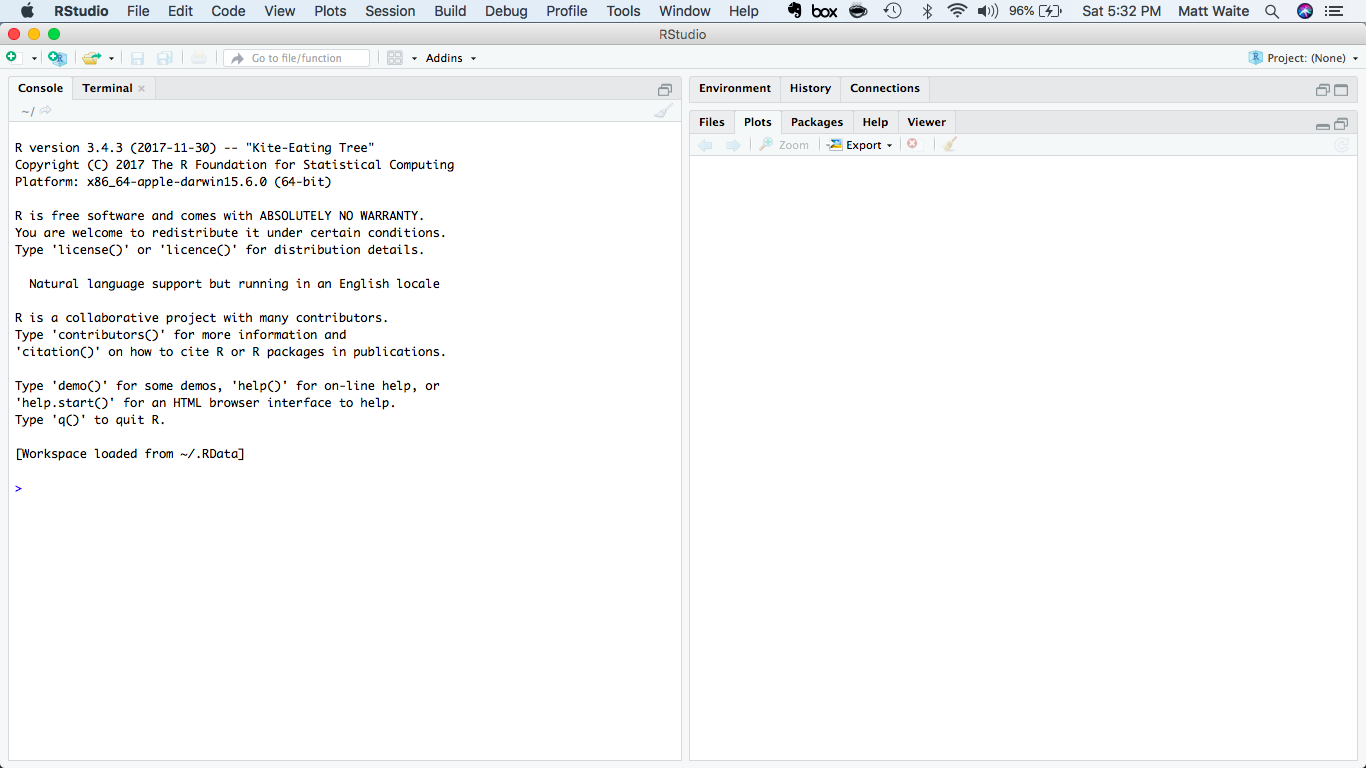
\includegraphics[width=18.97in]{images/verybasics1}

Think of the console like talking directly to R. It's direct, but it has some drawbacks and some quirks we'll get into later. For now, try typing this into the console and hit enter:

\begin{Shaded}
\begin{Highlighting}[]
\DecValTok{2}\OperatorTok{+}\DecValTok{2}
\end{Highlighting}
\end{Shaded}

\begin{verbatim}
## [1] 4
\end{verbatim}

Congrats, you've run some code. It's not very complex, and you knew the answer before hand, but you get the idea. We can compute things. We can also store things. \textbf{In programming languages, these are called variables}. We can assign things to variables using \texttt{\textless{}-}. And then we can do things with them. \textbf{The \texttt{\textless{}-} is a called an assignment operator}.

Try this in your console.

\begin{Shaded}
\begin{Highlighting}[]
\NormalTok{number <-}\StringTok{ }\DecValTok{2}

\NormalTok{number }\OperatorTok{*}\StringTok{ }\NormalTok{number}
\end{Highlighting}
\end{Shaded}

\begin{verbatim}
## [1] 4
\end{verbatim}

Now assign a different number to the variable number. Try run \texttt{number\ *\ number} again. Get what you expected?

We can have as many variables as we can name. \textbf{We can even reuse them (but be careful you know you're doing that or you'll introduce errors)}. Try this in your console.

\begin{Shaded}
\begin{Highlighting}[]
\NormalTok{firstnumber <-}\StringTok{ }\DecValTok{1}
\NormalTok{secondnumber <-}\StringTok{ }\DecValTok{2} 

\NormalTok{(firstnumber }\OperatorTok{+}\StringTok{ }\NormalTok{secondnumber) }\OperatorTok{*}\StringTok{ }\NormalTok{secondnumber}
\end{Highlighting}
\end{Shaded}

\begin{verbatim}
## [1] 6
\end{verbatim}

\textbf{We can store anything in a variable}. A whole table. An array of numbers. A single word. A whole book. All the books of the 18th century. They're really powerful. We'll explore them at length.

\hypertarget{adding-libraries-part-1}{%
\section{Adding libraries, part 1}\label{adding-libraries-part-1}}

The real strength of any given programming language is the external libraries that power it. The base language can do a lot, but it's the external libraries that solve many specific problems -- even making the base language easier to use.

For this class, we're going to need several external libraries.

The first library we're going to use is called Swirl. So in the console, type \texttt{install.packages(\textquotesingle{}swirl\textquotesingle{})} and hit enter. That installs swirl.

Now, to use the library, type \texttt{library(swirl)} and hit enter. That loads swirl. Then type \texttt{swirl()} and hit enter. Now you're running swirl. Follow the directions on the screen. When you are asked, you want to install course 1 R Programming: The basics of programming in R. Then, when asked, you want to do option 1, R Programming, in that course.

When you are finished with the course -- it will take just a few minutes -- type 0 to exit (it will not be clear that's what you do when you are done).

\hypertarget{adding-libraries-part-2}{%
\section{Adding libraries, part 2}\label{adding-libraries-part-2}}

We'll mostly use two libraries for analysis -- \texttt{dplyr} and \texttt{ggplot2}. To get them, and several other useful libraries, we can install a single collection of libraries called the tidyverse. Type this into your console: \texttt{install.packages(\textquotesingle{}tidyverse\textquotesingle{})}

\textbf{NOTE}: This is a pattern. You should always install libraries in the console.

Then, to help us with learning and replication, we're going to use R Notebooks. So we need to install that library. Type this into your console: \texttt{install.packages(\textquotesingle{}rmarkdown\textquotesingle{})}

\hypertarget{data-journalism-in-the-age-of-replication}{%
\chapter{Data journalism in the age of replication}\label{data-journalism-in-the-age-of-replication}}

It's a single word in a single job description, but a Buzzfeed job posting in 2017 is another indicator in what could be a profound shift in how data journalism is both practiced and taught.

``We're looking for someone with a passion for news and a commitment to using data to find amazing, important stories --- both quick hits and deeper analyses that drive conversations,'' the posting seeking a data journalist says. It goes on to list five things BuzzFeed is looking for: Excellent collaborator, clear writer, deep statistical understanding, knowledge of obtaining and restructuring data.

And then there's this:

\textbf{``You should have a strong command of at least one toolset that (a) allows for filtering, joining, pivoting, and aggregating tabular data, and (b) enables reproducible workflows.''}

The word you're seeing more and more of? Reproducible. And it started in earnest this summer when data journalism crossed a major threshold in American journalism: It now has it's own section in the Associated Press Stylebook.

``Data journalism has become a staple of reporting across beats and platforms,'' the Data Journalism section of the Stylebook opens. ``The ability to analyze quantitative information and present conclusions in an engaging and accurate way is no longer the domain of specialists alone.''

The AP's Data Journalism section discusses how to request data and in what format, guidelines for scraping data from websites with automation, the ethics of using leaked or hacked data and other topics long part of data journalism conference talks.

But the third page of the section contains perhaps the most profound commandment: \textbf{``As a general rule, all assertions in a story based on data analysis should be reproducible. The methodology description in the story or accompanying materials should provide a road map to replicate the analysis.''}

Reproducible research -- replication -- is a cornerstone of scientific inquiry. Researchers across a range of academic disciplines use methods to find new knowledge and publish it in peer reviewed journals. And, when it works, other researchers take that knowledge and try it with their own samples in their own locations. Replication studies exist to take something from an Interesting Finding to a Theory and beyond.

It doesn't always work.

Replication studies aren't funded at nearly the level as new research. And, to the alarm of many, scores of studies can't be replicated by others. Researchers across disciplines are finding that when their original studies are replicated, flaws are found, or the effects found aren't as strong as the original. Because of this, academics across a number of disciplines have written about a replication crisis in their respective fields, particularly psychology, social science and medical research.

In Chapter 1 of the New Precision Journalism, Phil Meyer wrote that ``we journalists would be wrong less often if we adapted to our own use some of the research tools of the social scientists.''

Meyer would go on to write about how computers pouring over datasets too large to crunch by hand had changed social science from a discipline with ``a few data and a lot of interpretation'' into a much more meaningful and powerful area of study. If journalists could become comfortable with data and some basic statistics, they too could harness this power.

``It used to be said that journalism is history in a hurry,'' Meyer wrote. ``The argument of this book is that to cope with the acceleration of social change in today's world, journalism must become social science in a hurry.''

He wrote that in 1971. It might as well have been yesterday.

Journalism doesn't have a history of replication, but the concerns about credibility are substantially greater. Trust in media is at an all time low and shows no signs of improving. While the politics of the day have quite a bit to do with this mistrust of media, being more transparent about what journalists do can't hurt.

The AP's commandment that Thou Must Replicate Your Findings could, if taken seriously by the news business, have substantial impacts on how data journalism gets done in newsrooms and how data journalism gets taught, both at professional conferences and universities.

How? Two ways.

\begin{itemize}
\tightlist
\item
  The predominant way that data journalism gets done in a newsroom is through simple tools like Microsoft Excel or Google Sheets. Those simple tools, on their own, lack significant logging functions, meaning journalists will have to maintain detailed logs of what they did so any analysis can be replicated.
\item
  The predominant way that data journalism gets taught -- both in professional settings and at most universities -- doesn't deal with replication at all. The tools and the training stress Getting Things Done -- an entirely logical focus for a deadline driven business. The choices of tools -- like spreadsheets -- are made to get from data to story as quick as possible, without frightening away math and tech phobic students.
\end{itemize}

If the AP's replication rules are to be followed, journalism needs to become much more serious about the tools and techniques used to do data journalism. The days of Point and Click tools to do Quick and Dirty analysis that get published are dying. The days of formal methods using documented steps are here.

\hypertarget{the-stylebook}{%
\section{The stylebook}\label{the-stylebook}}

Troy Thibodeaux, the editor of the AP's data journalism team, said the stylebook entry started when the data team found themselves answering the same questions over and over. With a grant from the Knight Foundation, the team began to document their own standards and turn that into a stylebook section.

From the beginning, they had a fairly clear idea of what they wanted to do -- think through a project and ask what the frequently asked questions are that came up. It was not going to be a soup-to-nuts guide to how to do a data project.

When the section came out, eyebrows went up on the replication parts, surprising Thibodeaux.

``From our perspective, this is a core value for us,'' he said. ``Just for our own benefit, we need to be able to have someone give us a second set of eyes. We benefit from that every day. We catch things for each other.''

Thibodeaux said the AP data team has two audiences when it comes to replication -- they have the readers of the work, and members of the collective who may want to do their own work with the data.

``This is something that's essential to the way we work,'' he said. ``And it's important in terms of transparency and credibility going forward. We thought it would be kind of unexceptionable.''

\hypertarget{replication}{%
\section{Replication}\label{replication}}

Meyer, now 86, said he's delighted to see replication up for discussion now, but warned that we shouldn't take it too far.

``Making the analysis replicable was something I worried about from the very beginning,'' he wrote in an email. So much so that in 1967, after publishing stories from his landmark survey after the Detroit riots, he shipped the data and backup materials about it to a social science data repository at the University of North Carolina.

And, in doing so, he opened the door to others replicating his results. One scholar attempted to find fault with Meyer's analysis by slicing the data ever thinner until the differences weren't significant -- gaming the analysis to criticize the stories.

Meyer believes replication is vitally important, but doesn't believe it should take on the trappings of science replication, where newsrooms take their own samples or re-survey a community. That would be prohibitively expensive.

But journalists should be sharing their data and analysis steps. And it doesn't need to be complicated, he said.

``Replication is a theoretical standard, not a requirement that every investigator duplicate his or her own work for every project,'' he said. ``Giving enough information in the report to enable another investigator to follow in your footsteps is enough. Just telling enough to make replication possible will build confidence.''

But as simple as that sounds, it's not so simple. Ask social scientists.

Andrew Gelman, a professor of statistics and political science and director of the Applied Statistics Center at Columbia University, wrote in the journal CHANCE in February that difficulties with replication in empirical research are pervasive.

``When an outsider requests data from a published paper, the authors will typically not post or send their data files and code, but instead will point to their sources, so replicators have to figure out exactly what to do from there,'' Gelman wrote. ``End-to-end replicability is not the norm, even among scholars who actively advocate for the principles of open science.''

So goes science, so goes journalism.

Until a recent set of exceptions, journalists rarely shared data. The ``nerd box'' -- a sidebar story that explains how a news organization did what they did -- is a term that first appeared on NICAR-L, a email listserv of data journalists, in the 1990s.

It was a form born in print.

As newsrooms adapted to the internet, some news organizations began linking to their data sources if they were online. Often, the data used in stories were obtained through records requests. Sometimes, reporters created the data themselves.

Journalism, more explicitly than science, is a competitive business. There have been arguments that nerd boxes and downloadable links give too much away to competitors.

Enter the AP Stylebook.

The AP Stylebook argues explicitly for both internal and external replication. Externally, they argue that the \textbf{``methodology description in the story or accompanying materials should provide a road map to replicate the analysis''}, meaning someone else could do the replication post publication.

Internally, the AP Stylebook says: \textbf{``If at all possible, an editor or another reporter should attempt to reproduce the results of the analysis and confirm all findings before publication.''}

There are two problems here.

First is that journalism, unlike science, has no history of replication. There is no Scientific Method for stories. There is no Research Methods class taught at every journalism school, at least not where it comes to writing stories. And, beyond that, journalism school isn't a requirement to get into the news business. In other words, journalism lacks the standards other disciplines have.

The second problem is, in many ways, worse: Except for the largest newsrooms, most news organizations lack editors who could replicate the analysis. Many don't have a second person who would know what to do.

Not having a second set of eyes in a newsroom is a problem, Thibodeaux acknowledges. Having a data journalism team ``is an incredible luxury'' at the AP, he said, and their rule is nothing goes on the wire without a second set of eyes.

Thibodeaux, for his part, wants to see fewer ``lone nerds in the corner'' -- it's too much pressure. That person gets too much credibility from people who don't understand what they do, and they get too much blame when a mistake is made.

So what would replication look like in a newsroom? What does this mean for how newsrooms do data journalism on deadline? And what does this mean for how data journalism is being taught, particularly at a time when only half of accredited journalism programs teach any data journalism at all?

Are we walking ourselves into our own replication crisis?

\hypertarget{goodbye-excel}{%
\section{Goodbye Excel?}\label{goodbye-excel}}

For decades, Excel has been the gateway drug for data journalists, the Swiss Army knife of data tools, the One Tool You Can't Live Without. Investigative Reporters and Editors, an organization that trains investigative journalists, have built large amounts of their curricula around Excel. Of the journalism schools that teach data journalism, most of them begin and end with spreadsheets.

The Stylebook says at a minimum, today's data journalists should keep a log that details:

\begin{itemize}
\tightlist
\item
  The source of the data, making sure to work on a copy of the data and not the original file.
\item
  Data dictionaries or any other supporting documentation of the data.
\item
  \textbf{``Description of all steps required to transform the data and perform the analysis.''}
\end{itemize}

The trouble with Excel is, unless you are keeping meticulous notes on what steps you are taking, there's no way to keep track. Many data journalists will copy and paste the values of a formula over the formula itself to prevent Excel from fouling up cell references when moving data around -- a practical step that also cuts off another path to being able to replicate the results.

An increasing number of data journalists are switching to tools like analysis notebooks, which use languages like Python and R, to document their work. The notebooks, generally speaking, allow a data journalist to mix code and explanation in the same document.

Combined with online sharing tools like GitHub, analysis notebooks seem to solve the problem of replication. But the number using them is small compared to those using spreadsheets. Recent examples of news organizations using analysis notebooks include the \href{https://github.com/datadesk}{Los Angeles Times}, the \href{https://github.com/TheUpshot}{New York Times}, \href{https://github.com/fivethirtyeight/data}{FiveThirtyEight}, and \href{https://github.com/BuzzFeedNews}{Buzzfeed}.

Peter Aldous, a data journalist at Buzzfeed recently published a story about how the online news site used machine learning to find airplanes being used to spy on people in American cities. Published with the story is the code Aldous used to build his case.

``I think of it this way: As a journalist, I don't like to simply trust what people tell me. Sometimes sources lie. Sometimes they're just mistaken. So I like to verify what I'm told,'' he wrote in an email. ``By the same token, why should someone reading one of my articles believe my conclusions, if I don't provide the evidence that explains how I reached them?''

The methodology document, associated code and source data took Aldous a few hours to create. The story, from the initial data work through the reporting required to make sense of it all, took a year. Aldous said there wasn't a discussion about if the methodology would be published because it was assumed -- ``it's written into our DNA at BuzzFeed News.''

``My background is in science journalism, and before that (way back in the 1980s) in science,'' Aldous said. ``In science, there's been a shift from descriptive methods sections to publishing data and analysis code for reproducible research. And I think we're seeing a similar shift in data journalism. Simply saying what you've done is not as powerful as providing the means for others to repeat and build on your work.''

Thibodeaux said that what Buzzfeed and others do with analysis notebooks and code repositories that include their data is ``lovely.''

``That to me is the shining city on the hill,'' Thibodeaux said. ``We're not going to get there, and I don't think we have to for every story and every use case, and I don't think it's necessarily practical for every person working with data to get to that point.''

There's a wide spectrum of approaches that still gets journalists to the essence of what the stylebook is trying to do, Thibodeaux said. There are many tools, many strategies, and the AP isn't going to advocate for any single one of them, he said. They're just arguing for transparency and replicability, even if that means doing more work.

``There's a certain burden that comes with transparency,'' he said. ``And I think we have to accept that burden.''

The question, Thibodeaux said, is what is sufficient? What's enough transparency? What does someone need for replicability?

``Maybe we do have to set a higher standard -- the more critical the analysis is to the story, and the more complex that analysis is, that's going to push the bar on what is a sufficient methodology statement,'' he said. ``And it could end up being a whole code repo in order to just say, this isn't black magic, here's how we got it if you're so interested.''

\hypertarget{receptivity-is-high}{%
\section{``Receptivity \ldots{} is high''}\label{receptivity-is-high}}

Though written almost half a century ago, Meyer foresaw how data journalism was going to arrive in the newsroom.

``For the new methods to gain currency in journalism, two things must happen,'' he wrote. ``Editors must feel the need strongly enough to develop the in-house capacity for systematic research \ldots{} The second need, of course, is for the editors to be able to find the talent to fill this need.''

Meyer optimistically wrote that journalism schools were prepared to provide that talent -- they were not then, and only small handful are now -- but students were unlikely to be drawn to these new skills if they didn't see a chance to use those skills in their careers.

It's taken 45 years, but we are now at this point.

``The potential for receptivity, especially among the younger generation of newspaper managers, is high,'' Meyer wrote.

\hypertarget{replication-in-notebooks}{%
\section{Replication in notebooks}\label{replication-in-notebooks}}

For our purposes in this book, replication requires two things from you, the student: What and why. What is this piece of code doing, and why are you doing that here and now? What lead you to this place? That you can copy and paste code from this book or the internet is not impressive. What is necessary for learning is that you know what a piece of code is doing a thing and why you want to do that thing here.

In an R Notebook, there are two blocks: A block that uses markdown, which has no special notation, and a code block. The code blocks can run mulitple languages inside R Studio, including Python, a general purpose scripting language; and SQL, or Structured Query Language, the language of databases.

For the rest of the class, we're going to be working in notebooks. In notebooks, you will both run your code and explain each step, much as I am doing here.

To start a notebook, you click on the green plus in the top left corner and go down to R Notebook. Do that now.


\includegraphics[width=11.08in]{images/verybasics2}

You will see that the notebook adds a lot of text for you. It tells you how to work in notebooks -- and you should read it. The most important parts are these:

To add text, simply type. To add code you can click on the \emph{Insert} button on the toolbar or by pressing \emph{Cmd+Option+I} on Mac or \emph{Ctl+Alt+I} on Windows.

Highlight all that text and delete it. You should have a blank document. This document is called a R Markdown file -- it's a special form of text, one that you can style, and one you can include R in the middle of it. Markdown is a simple markup format that you can use to create documents. So first things first, let's give our notebook a big headline. Add this:

\texttt{\#\ My\ awesome\ notebook}

Now, under that, without any markup, just type This is my awesome notebook.

Under that, you can make text bold by writing \texttt{It\ is\ **really**\ awesome}.

If you want it italics, just do this on the next line: \texttt{No,\ it\textquotesingle{}s\ \_really\_\ awesome.\ I\ swear.}

To see what it looks like without the markup, click the Preview or Knit button in the toolbar. That will turn your notebook into a webpage, with the formatting included.

Throughout this book, we're going to use this markdown to explain what we are doing and, more importantly, why we are doing it. Explaining your thinking is a vital part of understanding what you are doing.

That explaination, plus the code, is the real power of notebooks. To add a block of code, follow the instructions from above: click on the \emph{Insert} button on the toolbar or by pressing \emph{Cmd+Option+I} on Mac or \emph{Ctl+Alt+I} on Windows.

In that window, use some of the code from above and add two numbers together. To see it run, click the green triangle on the right. That runs the chunk. You should see the answer to your addition problem.

And that, just that, is the foundation you need to start this book.

\hypertarget{data-structures-and-types}{%
\chapter{Data, structures and types}\label{data-structures-and-types}}

Data are everywhere (and data is plural of datum, thus the use of are in that statement). It surrounds you. Every time you use your phone, you are creating data. Lots of it. Your online life. Any time you buy something. It's everywhere. News, like life, is no different. Modernity is drowning in data, and more comes along all the time.

In news, and in this class, we'll be dealing largely with two kinds of data: \textbf{event level data and summary data}. It's not hard to envision event level data. A car accident. A crime. A fire. They are the events that make up the whole. Combine them together -- summarize them -- and you'll have some notion of how the year went. What we usually see is summary data -- who wants to scroll through 365 days of crime data to figure out if crime was up or down?

To start with, we need to understand the shape of data.

\hypertarget{rows-and-columns}{%
\section{Rows and columns}\label{rows-and-columns}}

Data, oversimplifying it a bit, is information organized. Generally speaking, it's organized into rows and columns. Rows, generally, are individual elements. A crime. A county. An accident. Columns, generally, are components of the data, sometimes called variables. So if each row is a crime, the first column might be the type. The second is the date and time. The third is the location. And so on.

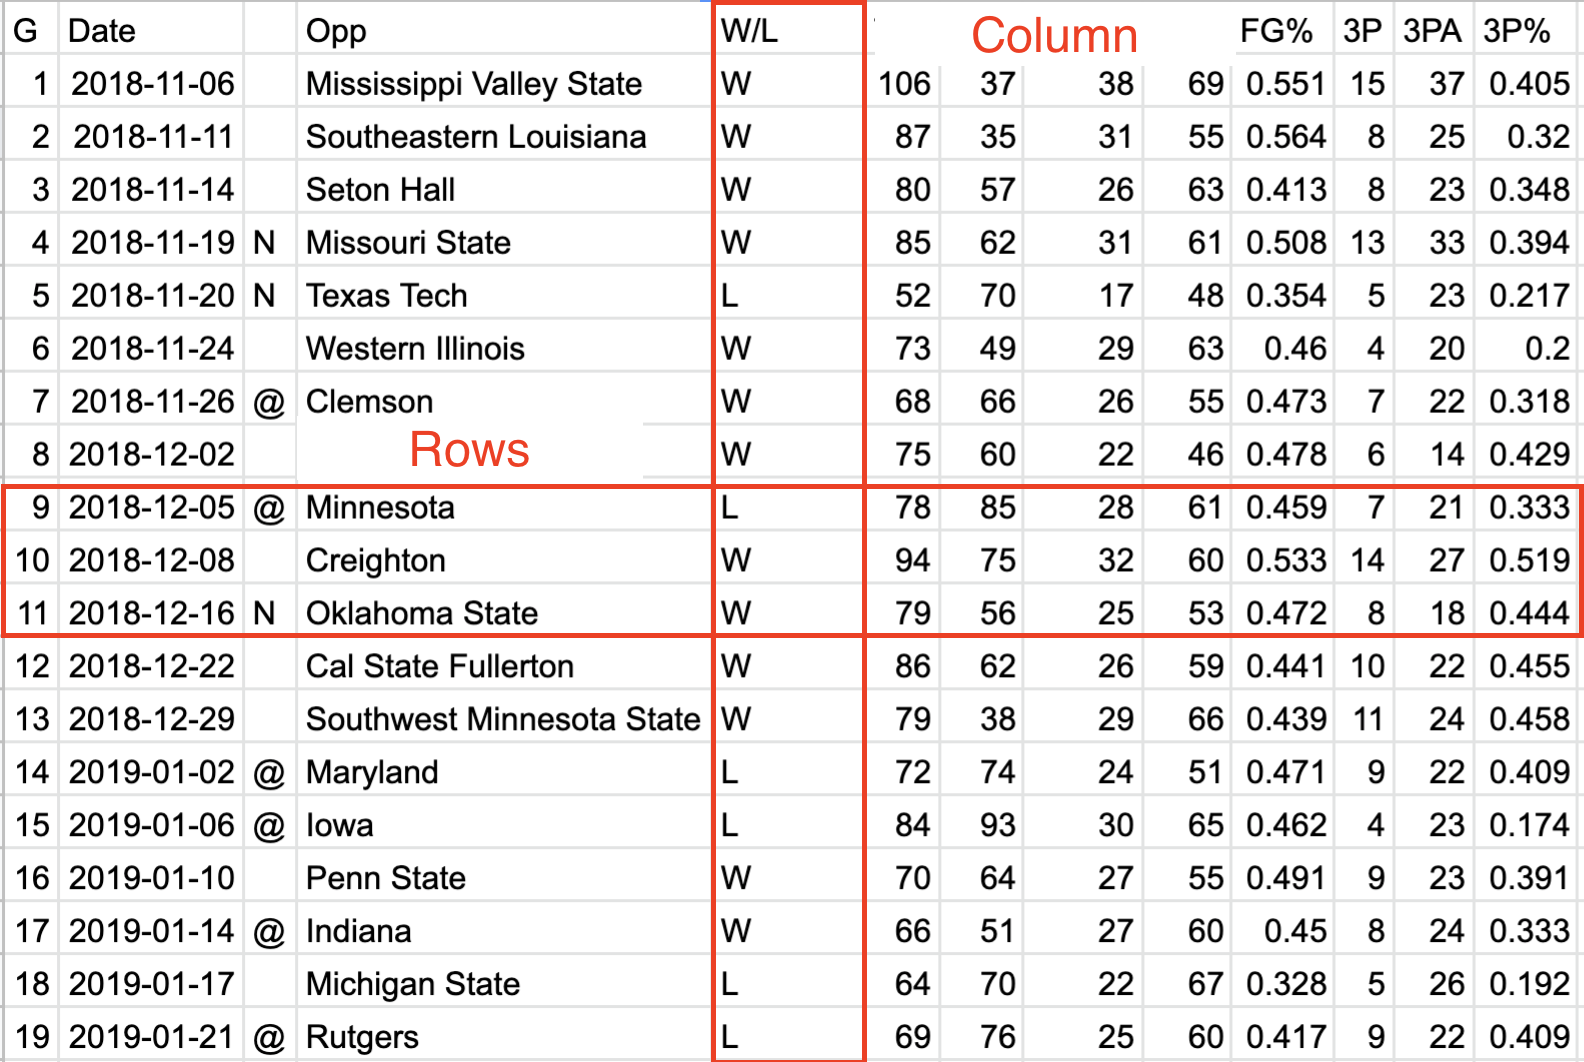
\includegraphics[width=22in]{images/data1}

One of the critical components of data analysis, especially for beginners, is having a mental picture of your data. What does each row mean? What does each column in each row signify? How many rows do you have? How many columns?

\begin{quote}
EXERCISE: I love orange Skittles. What are my chances of getting more orange Skittles than other colors in a fun sized packet? Each person in the class must track their package and everyone else using a spreadsheet. What differences between sheets emerge? What similarities?
\end{quote}

\hypertarget{types}{%
\section{Types}\label{types}}

There are scores of data types in the world, and R has them. In this class, we're primarily going to be dealing with data frames, and each element of our data frames will have a data type.

Typically, they'll be one of four types of data:

\begin{itemize}
\tightlist
\item
  Numeric: a number, like the number of car accidents in a year or the number of journalism majors.
\item
  Character: Text, like a name, a county, a state.
\item
  Date: Fully formed dates -- 2019-01-01 -- have a special date type. Elements of a date, like a year (ex. 2019) are not technically dates, so they'll appear as numeric data types.
\item
  Logical: Rare(ish), but every now and then we'll have a data type that's Yes or No, True or False, etc.
\end{itemize}

\textbf{Question:} Is a zip code a number? Is a jersey number a number? Trick question, because the answer is no. Numbers are things we do math on. If the thing you want is not something you're going to do math on -- can you add two phone numbers together? -- then make it a character type. If you don't, most every software system on the planet will drop leading zeros. For example, every zip code in Boston starts with 0. If you record that as a number, your zip code will become a four digit number, which isn't a zip code anymore.

\hypertarget{a-simple-way-to-get-data}{%
\section{A simple way to get data}\label{a-simple-way-to-get-data}}

The hardest part of doing data journalism is often getting the data. In news, there's scores of organizations and agencies collecting data, and zero standards on how it's being collected.

If we're lucky -- huge IF in news -- the data we want is in a downloadable format. If we're a little less lucky, there's a way to get the data on the web. And maybe that data is in a simple table. If so, we can pull that data directly into Google Sheets.

The Lincoln Police Department publishes a daily summary of calls. Some days -- like when it snows -- that data becomes news. So let's pretend that it snowed today and we need to see how many accidents the Lincoln Police responded to and what percentage of their call load that represents.

Open a browser and go to the \href{http://cjis.lincoln.ne.gov/~lpd/cfstoday.htm}{LPD's log page}. Now, in a new tab, log into Google Docs/Drive and open a new spreadsheet. In the first cell of the first row, copy and paste this formula in:

\begin{verbatim}
=importHTML("http://cjis.lincoln.ne.gov/~lpd/cfstoday.htm","table",1)
\end{verbatim}

This is \textbf{function}, with three \textbf{inputs}. The function is \texttt{importHTML} and the three inputs in order are the url of the page, the HTML tag we're after (a

tag in our case) and the number of the tag you're after. So our function says go to the LPD page and get the first table tag you find. Fortunately for us, there's only one.

If your version worked right, you've got the data from that page in a spreadsheet.

\hypertarget{cleaning-the-data}{%
\section{Cleaning the data}\label{cleaning-the-data}}

The first thing we need to do is recognize that we don't have data, really. We have the results of a formula. You can tell by putting your cursor on that field, where you'll see the formula again. This is where you'd look:

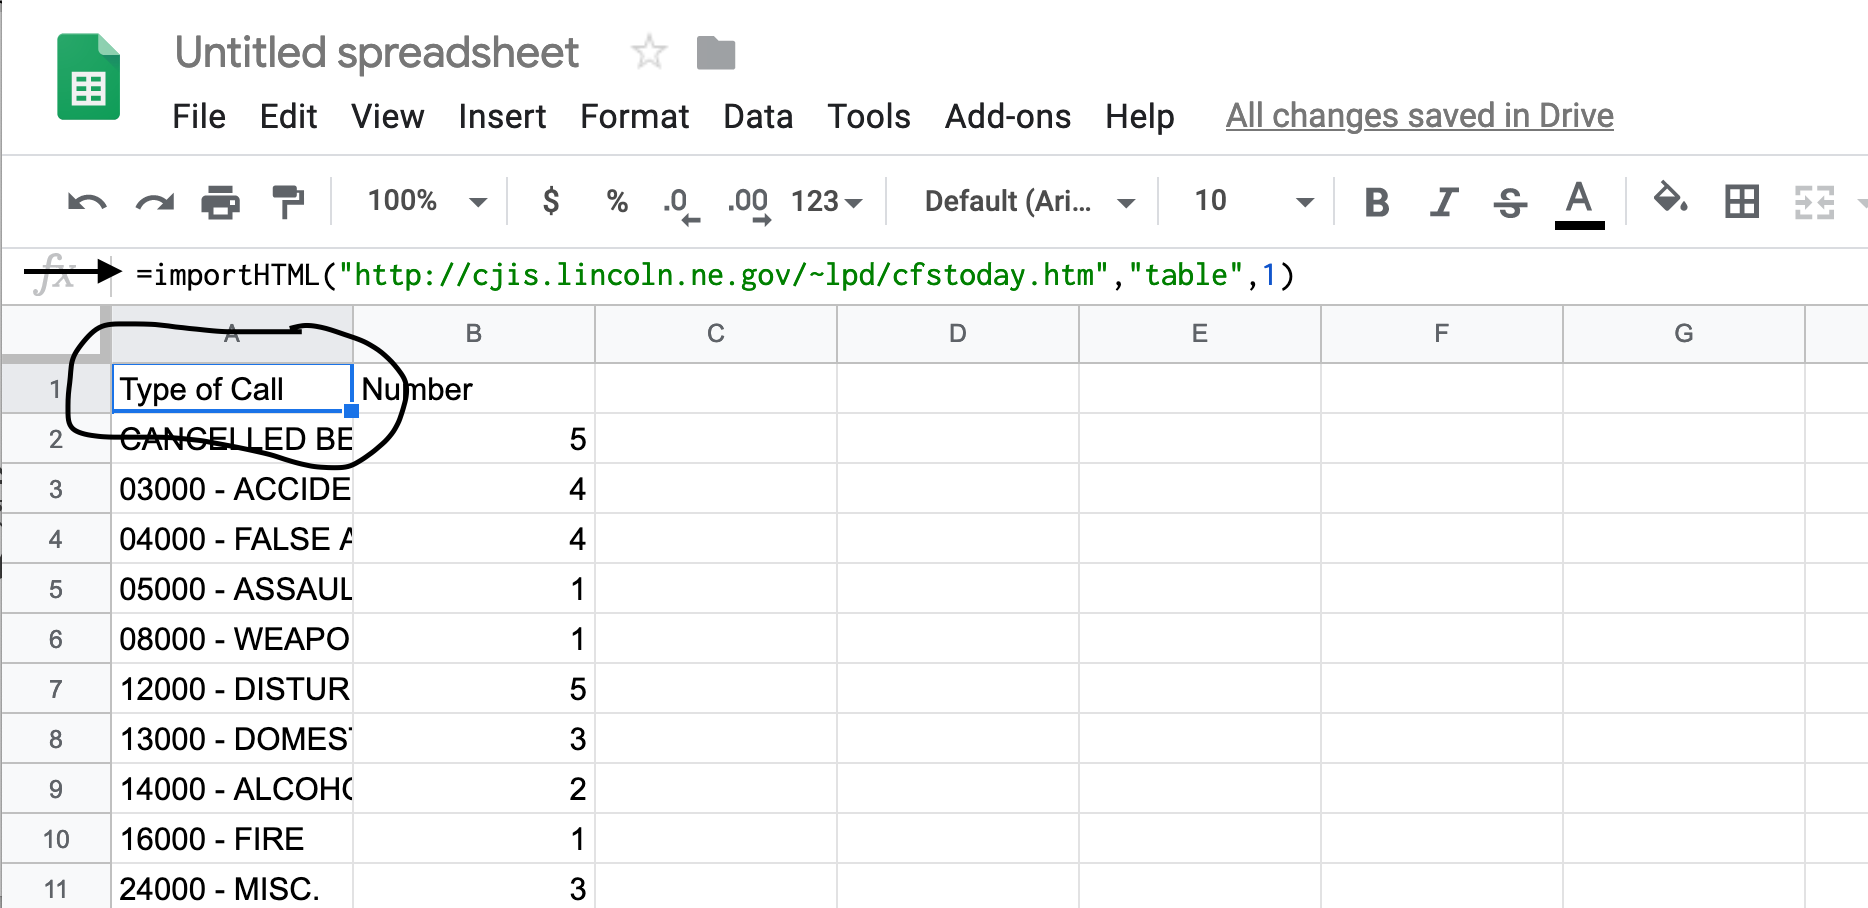
\includegraphics[width=25.94in]{images/clean1}

The solution is easy:

Edit \textgreater{} Select All or type command/control A
Edit \textgreater{} Copy or type command/control C
Edit \textgreater{} Paste Special \textgreater{} Values Only or type command/control shift V

You can verify that it worked by looking in that same row 1 column A, where you'll see the formula is gone.

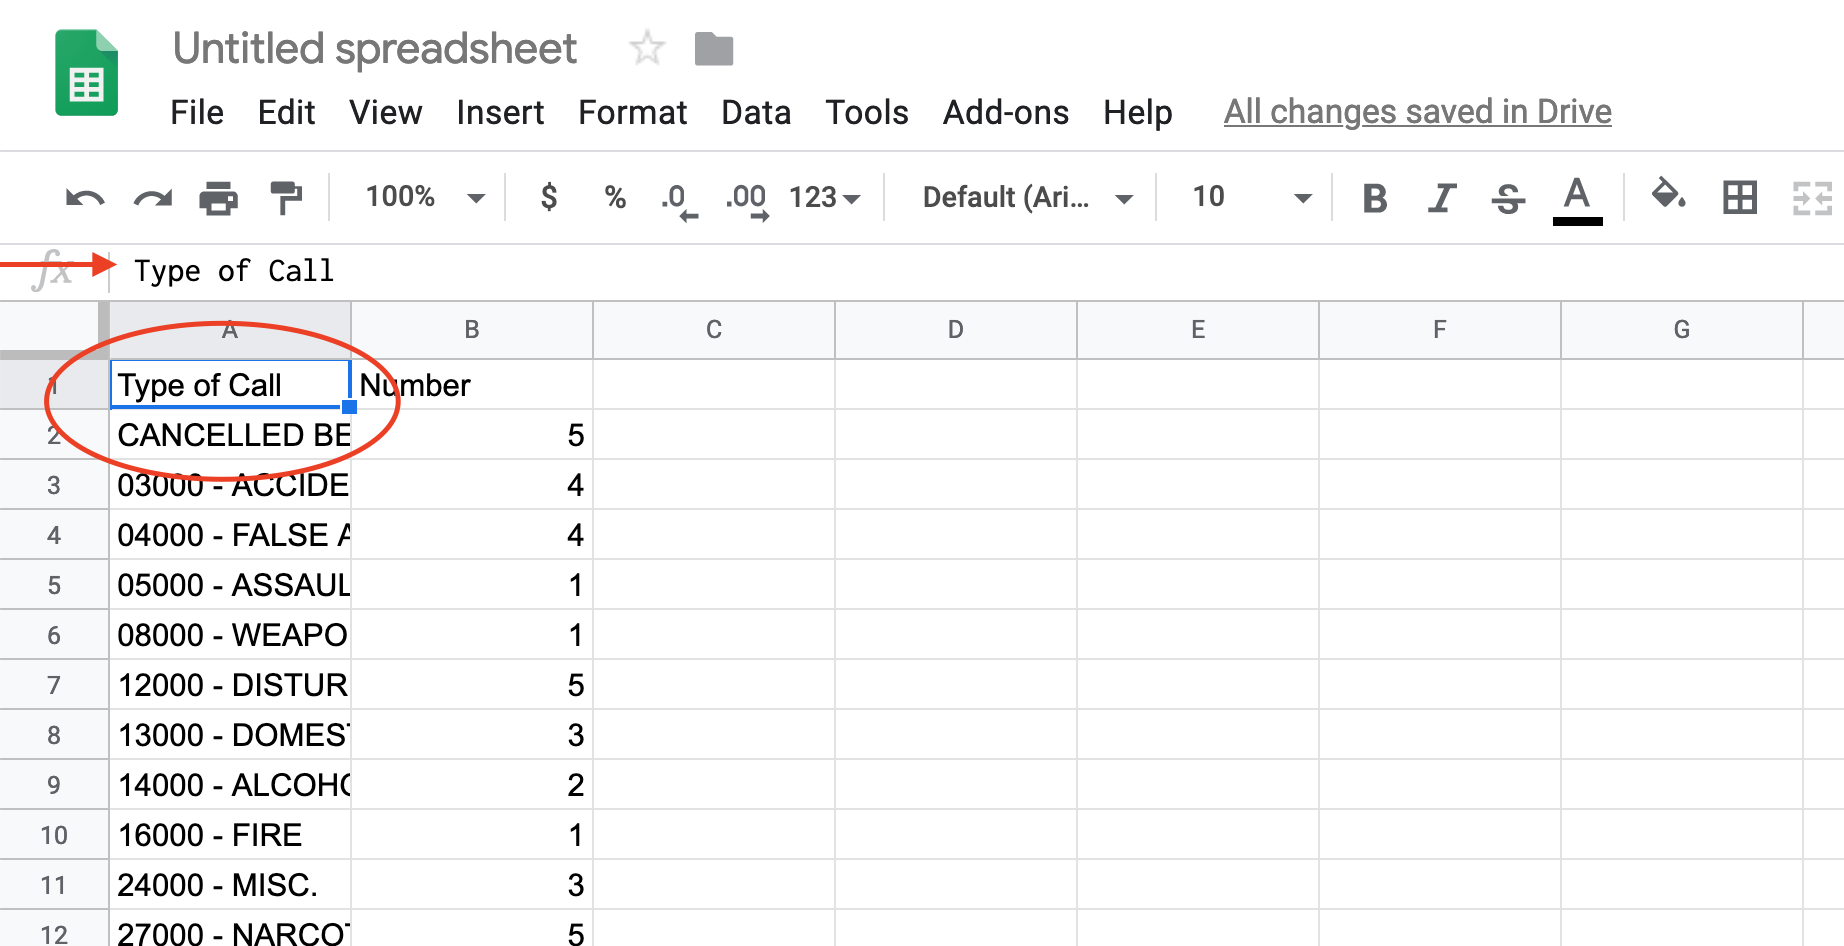
\includegraphics[width=25.61in]{images/clean2}

Now you have data, but look closely. At the bottom of the data, you have the total number of calls. More often than not, and particularly the deeper into this book we go, you want to delete that. So click on the number next to that Total Calls line to highlight it and go up to Edit \textgreater{} Delete Row XX where XX is the row number.

After you've done that, you can export it for use in R. Go to File \textgreater{} Download as \textgreater{} Comma Separated Values.

\hypertarget{aggregates}{%
\chapter{Aggregates}\label{aggregates}}

R is a statistical programming language that is purpose built for data analysis.

Base R does a lot, but there are a mountain of external libraries that do things to make R better/easier/more fully featured. We already installed the tidyverse -- or you should have if you followed the instructions for the last assignment -- which isn't exactly a library, but a collection of libraries. Together, they make up the tidyverse. Individually, they are extraordinarily useful for what they do. We can load them all at once using the tidyverse name, or we can load them individually. Let's start with individually.

The two libraries we are going to need for this assignment are \texttt{readr} and \texttt{dplyr}. The library \texttt{readr} reads different types of data in. For this assignment, we're going to read in csv data or Comma Separated Values data. That's data that has a comma between each column of data.

Then we're going to use \texttt{dplyr} to analyze it.

To use a library, you need to import it. Good practice -- one I'm going to insist on -- is that you put all your library steps at the top of your notebooks.

That code looks like this:

\begin{Shaded}
\begin{Highlighting}[]
\KeywordTok{library}\NormalTok{(readr)}
\end{Highlighting}
\end{Shaded}

To load them both, you need to do this:

\begin{Shaded}
\begin{Highlighting}[]
\KeywordTok{library}\NormalTok{(readr)}
\KeywordTok{library}\NormalTok{(dplyr)}
\end{Highlighting}
\end{Shaded}

But, because those two libraries -- and several others that we're going to use over the course of this class -- are so commonly used, there's a shortcut to loading all of the libraries we'll need:

\begin{Shaded}
\begin{Highlighting}[]
\KeywordTok{library}\NormalTok{(tidyverse)}
\end{Highlighting}
\end{Shaded}

You can keep doing that for as many libraries as you need. I've seen notebooks with 10 or more library imports.

\hypertarget{importing-data}{%
\section{Importing data}\label{importing-data}}

The first thing we need to do is get some data to work with. We do that by reading it in. In our case, we're going to read data from a csv file -- a comma-separated values file.

The CSV file we're going to read from is a \href{https://unl.box.com/s/xjipgkesl9rjmng4weg77vb73xt41apf}{Nebraska Game and Parks Commission dataset} of confirmed mountain lion sightings in Nebraska. There are, on occasion, fierce debates about mountain lions and if they should be hunted in Nebraska. This dataset can tell us some interesting things about that debate.

So step 1 is to import the data. The code looks \emph{something} like this, but hold off copying it just yet:

\texttt{mountainlions\ \textless{}-\ read\_csv("\textasciitilde{}/Documents/Data/mountainlions.csv")}

Let's unpack that.

The first part -- mountainlions -- is the name of your variable. A variable is just a name of a thing. In this case, our variable is a dataframe, which is R's way of storing data. We can call this whatever we want. I always want to name dataframes after what is in it. In this case, we're going to import a dataset of mountain lion sightings from the Nebraska Game and Parks Commission. \textbf{Variable names, by convention are one word all lower case}. You can end a variable with a number, but you can't start one with a number.

The \textless{}- bit, you'll recall from the basics, is the \textbf{variable assignment operator}. It's how we know we're assigning something to a word. Think of the arrow as saying ``Take everything on the right of this arrow and stuff it into the thing on the left.'' So we're creating an empty vessel called mountainlions and stuffing all this data into it.

The \texttt{read\_csv} bits are pretty obvious, except for one thing. What happens in the quote marks is the path to the data. In there, I have to tell R where it will find the data.

\begin{quote}
The easiest thing to do, if you are confused about how to find your data, is to put your data in the same folder as as your notebook (you'll have to save that notebook first). If you do that, then you just need to put the name of the file in there (mountainlions.csv).
\end{quote}

In my case, the file path I've got starts with a \textasciitilde{} character. That's a shortcut for my home directory. It's the same on your computer. Your home directory is where your Documents, Desktop and Downloads directories are. I've got a folder called Documents in my home directory, and in there is a folder called Data that has the file called mountainlions.csv in it. Thus, \texttt{\textasciitilde{}/Documents/Data/mountainlions.csv}

Some people -- insane people -- leave the data in their downloads folder. The data path then would be \texttt{\textasciitilde{}/Downloads/nameofthedatafilehere.csv} on PC or Mac.

A quick way to find your data file? The tab key. If you start your code \texttt{dataframenamehere\ \textless{}-\ read\_csv(")} and after typing the first quote mark you hit tab, it will show you the files in the folder you are in. With that, you can start to narrow in on where you need to go.

\textbf{So what you put in your import step will be different from mine}. Your first task is to import the data. Here's mine. Use the tab key to find your data file and get the correct path.

\begin{Shaded}
\begin{Highlighting}[]
\NormalTok{mountainlions <-}\StringTok{ }\KeywordTok{read_csv}\NormalTok{(}\StringTok{"data/mountainlions.csv"}\NormalTok{)}
\end{Highlighting}
\end{Shaded}

\begin{verbatim}
## Parsed with column specification:
## cols(
##   ID = col_double(),
##   `Cofirm Type` = col_character(),
##   COUNTY = col_character(),
##   Date = col_character()
## )
\end{verbatim}

Now we can inspect the data we imported. What does it look like? To do that, we use \texttt{head(mountainlions)} to \textbf{show the headers and the first six rows of data}. If we wanted to see them all, we could just simply enter \texttt{mountainlions} and run it.

To get the number of records in our dataset, we run \texttt{nrow(mountainlions)}

\begin{Shaded}
\begin{Highlighting}[]
\KeywordTok{head}\NormalTok{(mountainlions)}
\end{Highlighting}
\end{Shaded}

\begin{verbatim}
## # A tibble: 6 x 4
##      ID `Cofirm Type` COUNTY       Date    
##   <dbl> <chr>         <chr>        <chr>   
## 1     1 Track         Dawes        9/14/91 
## 2     2 Mortality     Sioux        11/10/91
## 3     3 Mortality     Scotts Bluff 4/21/96 
## 4     4 Mortality     Sioux        5/9/99  
## 5     5 Mortality     Box Butte    9/29/99 
## 6     6 Track         Scotts Bluff 11/12/99
\end{verbatim}

\begin{Shaded}
\begin{Highlighting}[]
\KeywordTok{nrow}\NormalTok{(mountainlions)}
\end{Highlighting}
\end{Shaded}

\begin{verbatim}
## [1] 393
\end{verbatim}

\hypertarget{group-by-and-count}{%
\section{Group by and count}\label{group-by-and-count}}

So what if we wanted to know how many mountain lion sightings there were in each county?

To do that by hand, we'd have to take each of the 393 records and sort them into a pile. We'd put them in groups and then count them.

\texttt{dplyr} has a group by function in it that does just this. A massive amount of data analysis involves grouping like things together and then doing simple things like counting them, or averaging them together. So it's a good place to start.

So to do this, we'll take our dataset and we'll introduce a new operator: \texttt{\%\textgreater{}\%}. The best way to read that operator, in my opinion, is to interpret that as ``and then do this.''

We're going to establish a pattern that will come up again and again throughout this book: \texttt{data\ \%\textgreater{}\%\ function}. The first step of every analysis starts with the data being used. Then we apply functions to the data.

In our case, the pattern that you'll use many, many times is: \texttt{data\ \%\textgreater{}\%\ group\_by(FIELD\ NAME)\ \%\textgreater{}\%\ summarize(VARIABLE\ NAME\ =\ AGGREGATE\ FUNCTION(FIELD\ NAME))}

Here's the code:

\begin{Shaded}
\begin{Highlighting}[]
\NormalTok{mountainlions }\OperatorTok
\StringTok{  }\KeywordTok{group_by}\NormalTok{(COUNTY) }\OperatorTok
\StringTok{  }\KeywordTok{summarise}\NormalTok{(}
    \DataTypeTok{total =} \KeywordTok{n}\NormalTok{()}
\NormalTok{  )}
\end{Highlighting}
\end{Shaded}

\begin{verbatim}
## # A tibble: 42 x 2
##    COUNTY    total
##    <chr>     <int>
##  1 Banner        6
##  2 Blaine        3
##  3 Box Butte     4
##  4 Brown        15
##  5 Buffalo       3
##  6 Cedar         1
##  7 Cherry       30
##  8 Custer        8
##  9 Dakota        3
## 10 Dawes       111
## # ... with 32 more rows
\end{verbatim}

So let's walk through that. We start with our dataset -- \texttt{mountainlions} -- and then we tell it to group the data by a given field in the data. In this case, we wanted to group together all the counties, signified by the field name COUNTY, which you could get from looking at \texttt{head(mountainlions)}. After we group the data, we need to count them up. In dplyr, we use \texttt{summarize} \href{http://dplyr.tidyverse.org/reference/summarise.html}{which can do more than just count things}. Inside the parentheses in summarize, we set up the summaries we want. In this case, we just want a count of the counties: \texttt{total\ =\ n(),} says create a new field, called \texttt{total} and set it equal to \texttt{n()}, which might look weird, but it's common in stats. The number of things in a dataset? Statisticians call in n. There are n number of incidents in this dataset. So \texttt{n()} is a function that counts the number of things there are.

And when we run that, we get a list of counties with a count next to them. But it's not in any order. So we'll add another And Then Do This \%\textgreater{}\% and use \texttt{arrange}. Arrange does what you think it does -- it arranges data in order. By default, it's in ascending order -- smallest to largest. But if we want to know the county with the most mountain lion sightings, we need to sort it in descending order. That looks like this:

\begin{Shaded}
\begin{Highlighting}[]
\NormalTok{mountainlions }\OperatorTok
\StringTok{  }\KeywordTok{group_by}\NormalTok{(COUNTY) }\OperatorTok
\StringTok{  }\KeywordTok{summarise}\NormalTok{(}
    \DataTypeTok{count =} \KeywordTok{n}\NormalTok{()}
\NormalTok{  ) }\OperatorTok\StringTok{ }\KeywordTok{arrange}\NormalTok{(}\KeywordTok{desc}\NormalTok{(count))}
\end{Highlighting}
\end{Shaded}

\begin{verbatim}
## # A tibble: 42 x 2
##    COUNTY       count
##    <chr>        <int>
##  1 Dawes          111
##  2 Sioux           52
##  3 Sheridan        35
##  4 Cherry          30
##  5 Scotts Bluff    26
##  6 Keya Paha       20
##  7 Brown           15
##  8 Rock            11
##  9 Lincoln         10
## 10 Custer           8
## # ... with 32 more rows
\end{verbatim}

We can, if we want, group by more than one thing. So how are these sightings being confirmed? To do that, we can group by County and ``Cofirm Type'', which is how the state misspelled Confirm. But note something in this example below:

\begin{Shaded}
\begin{Highlighting}[]
\NormalTok{mountainlions }\OperatorTok
\StringTok{  }\KeywordTok{group_by}\NormalTok{(COUNTY, }\StringTok{`}\DataTypeTok{Cofirm Type}\StringTok{`}\NormalTok{) }\OperatorTok
\StringTok{  }\KeywordTok{summarise}\NormalTok{(}
    \DataTypeTok{count =} \KeywordTok{n}\NormalTok{()}
\NormalTok{  ) }\OperatorTok\StringTok{ }\KeywordTok{arrange}\NormalTok{(}\KeywordTok{desc}\NormalTok{(count))}
\end{Highlighting}
\end{Shaded}

\begin{verbatim}
## # A tibble: 93 x 3
## # Groups:   COUNTY [42]
##    COUNTY       `Cofirm Type`      count
##    <chr>        <chr>              <int>
##  1 Dawes        Trail Camera Photo    41
##  2 Sioux        Trail Camera Photo    40
##  3 Dawes        Track                 19
##  4 Keya Paha    Trail Camera Photo    18
##  5 Cherry       Trail Camera Photo    17
##  6 Dawes        Mortality             17
##  7 Sheridan     Trail Camera Photo    16
##  8 Dawes        Photo                 13
##  9 Dawes        DNA                   11
## 10 Scotts Bluff Trail Camera Photo    11
## # ... with 83 more rows
\end{verbatim}

See it? When you have a field name that has two words, \texttt{readr} wraps it in back ticks, which is next to the 1 key on your keyboard. You can figure out which fields have back ticks around it by looking at the output of \texttt{readr}. Pay attention to that, because it's coming up again in the next section and will be a part of your homework.

\hypertarget{other-aggregates-mean-and-median}{%
\section{Other aggregates: Mean and median}\label{other-aggregates-mean-and-median}}

In the last example, we grouped some data together and counted it up, but there's so much more you can do. You can do multiple measures in a single step as well.

Let's look at some \href{https://unl.box.com/s/09t2u4qoncfh6qlv2156flzlxb8ruzpq}{salary data from the University of Nebraska}.

\begin{Shaded}
\begin{Highlighting}[]
\NormalTok{salaries <-}\StringTok{ }\KeywordTok{read_csv}\NormalTok{(}\StringTok{"data/nusalaries1819.csv"}\NormalTok{)}
\end{Highlighting}
\end{Shaded}

\begin{verbatim}
## Parsed with column specification:
## cols(
##   Employee = col_character(),
##   Position = col_character(),
##   Campus = col_character(),
##   Department = col_character(),
##   `Budgeted Annual Salary` = col_number(),
##   `Salary from State Aided Funds` = col_number(),
##   `Salary from Other Funds` = col_number()
## )
\end{verbatim}

\begin{Shaded}
\begin{Highlighting}[]
\KeywordTok{head}\NormalTok{(salaries)}
\end{Highlighting}
\end{Shaded}

\begin{verbatim}
## # A tibble: 6 x 7
##   Employee Position Campus Department `Budgeted Annua~ `Salary from St~
##   <chr>    <chr>    <chr>  <chr>                 <dbl>            <dbl>
## 1 Abbey, ~ Associa~ UNK    Kinesiolo~            61276            61276
## 2 Abbott,~ Staff S~ UNL    FM&P Faci~            37318               NA
## 3 Abboud,~ Adminis~ UNMC   Surgery-U~            76400            76400
## 4 Abdalla~ Asst Pr~ UNMC   Pathology~            74774            71884
## 5 Abdelka~ Post-Do~ UNMC   Surgery-T~            43516               NA
## 6 Abdel-M~ Researc~ UNL    Public Po~            58502               NA
## # ... with 1 more variable: `Salary from Other Funds` <dbl>
\end{verbatim}

In summarize, we can calculate any number of measures. Here, we'll use R's built in mean and median functions to calculate \ldots{} well, you get the idea.

\begin{Shaded}
\begin{Highlighting}[]
\NormalTok{salaries }\OperatorTok
\StringTok{  }\KeywordTok{summarise}\NormalTok{(}
    \DataTypeTok{count =} \KeywordTok{n}\NormalTok{(),}
    \DataTypeTok{mean_salary =} \KeywordTok{mean}\NormalTok{(}\StringTok{`}\DataTypeTok{Budgeted Annual Salary}\StringTok{`}\NormalTok{),}
    \DataTypeTok{median_salary =} \KeywordTok{median}\NormalTok{(}\StringTok{`}\DataTypeTok{Budgeted Annual Salary}\StringTok{`}\NormalTok{)}
\NormalTok{  )}
\end{Highlighting}
\end{Shaded}

\begin{verbatim}
## # A tibble: 1 x 3
##   count mean_salary median_salary
##   <int>       <dbl>         <dbl>
## 1 13039      62065.         51343
\end{verbatim}

So there's 13,039 employees in the database, spread across four campuses plus the system office. The mean or average salary is about \$62,000, but the median salary is slightly more than \$51,000.

Why?

Let's let sort help us.

\begin{Shaded}
\begin{Highlighting}[]
\NormalTok{salaries }\OperatorTok\StringTok{ }\KeywordTok{arrange}\NormalTok{(}\KeywordTok{desc}\NormalTok{(}\StringTok{`}\DataTypeTok{Budgeted Annual Salary}\StringTok{`}\NormalTok{))}
\end{Highlighting}
\end{Shaded}

\begin{verbatim}
## # A tibble: 13,039 x 7
##    Employee Position Campus Department `Budgeted Annua~ `Salary from St~
##    <chr>    <chr>    <chr>  <chr>                 <dbl>            <dbl>
##  1 Frost, ~ Head Co~ UNL    Athletics           5000000               NA
##  2 Miles, ~ Head Co~ UNL    Athletics           2375000               NA
##  3 Moos, W~ Athleti~ UNL    Athletics           1000000               NA
##  4 Gold, J~ Chancel~ UNMC   Office of~           853338           853338
##  5 Chinand~ Assista~ UNL    Athletics            800000               NA
##  6 Walters~ Assista~ UNL    Athletics            700000               NA
##  7 Cook, J~ Head Co~ UNL    Athletics            675000               NA
##  8 William~ Head Co~ UNL    Athletics            626750               NA
##  9 Bounds,~ Preside~ UNCA   Office of~           540000           540000
## 10 Austin ~ Assista~ UNL    Athletics            475000               NA
## # ... with 13,029 more rows, and 1 more variable: `Salary from Other
## #   Funds` <dbl>
\end{verbatim}

Oh, right. In this dataset, the university pays a football coach \$5 million. Extremes influence averages, not medians, and now you have your answer.

So when choosing a measure of the middle, you have to ask yourself -- could I have extremes? Because a median won't be sensitive to extremes. It will be the point at which half the numbers are above and half are below. The average or mean will be a measure of the middle, but if you have a bunch of low paid people and then one football coach, the average will be wildly skewed. Here, because there's so few highly paid football coaches compared to people who make a normal salary, the number is only slightly skewed in the grand scheme, but skewed nonetheless.

\hypertarget{even-more-aggregates}{%
\section{Even more aggregates}\label{even-more-aggregates}}

There's a ton of things we can do in summarize -- we'll work with more of them as the course progresses -- but here's a few other questions you can ask.

Which department on campus has the highest wage bill? And what is the highest and lowest salary in the department? And how wide is the spread between salaries? We can find that with \texttt{sum} to add up the salaries to get the total wage bill, \texttt{min} to find the minumum salary, \texttt{max} to find the maximum salary and \texttt{sd} to find the standard deviation in the numbers.

\begin{Shaded}
\begin{Highlighting}[]
\NormalTok{salaries }\OperatorTok\StringTok{ }
\StringTok{  }\KeywordTok{group_by}\NormalTok{(Campus, Department) }\OperatorTok\StringTok{ }
\StringTok{  }\KeywordTok{summarize}\NormalTok{(}
    \DataTypeTok{total =} \KeywordTok{sum}\NormalTok{(}\StringTok{`}\DataTypeTok{Budgeted Annual Salary}\StringTok{`}\NormalTok{), }
    \DataTypeTok{avgsalary =} \KeywordTok{mean}\NormalTok{(}\StringTok{`}\DataTypeTok{Budgeted Annual Salary}\StringTok{`}\NormalTok{), }
    \DataTypeTok{minsalary =} \KeywordTok{min}\NormalTok{(}\StringTok{`}\DataTypeTok{Budgeted Annual Salary}\StringTok{`}\NormalTok{),}
    \DataTypeTok{maxsalary =} \KeywordTok{max}\NormalTok{(}\StringTok{`}\DataTypeTok{Budgeted Annual Salary}\StringTok{`}\NormalTok{),}
    \DataTypeTok{stdev =} \KeywordTok{sd}\NormalTok{(}\StringTok{`}\DataTypeTok{Budgeted Annual Salary}\StringTok{`}\NormalTok{)) }\OperatorTok\StringTok{ }\KeywordTok{arrange}\NormalTok{(}\KeywordTok{desc}\NormalTok{(total))}
\end{Highlighting}
\end{Shaded}

\begin{verbatim}
## # A tibble: 804 x 7
## # Groups:   Campus [5]
##    Campus Department                  total avgsalary minsalary maxsalary  stdev
##    <chr>  <chr>                       <dbl>     <dbl>     <dbl>     <dbl>  <dbl>
##  1 UNL    Athletics                  3.56e7   118508.     12925   5000000 3.33e5
##  2 UNMC   Pathology/Microbiology     1.36e7    63158.      1994    186925 3.41e4
##  3 UNL    Agronomy & Horticulture    8.98e6    66496.      5000    208156 4.01e4
##  4 UNMC   Anesthesiology             7.90e6    78237.     10000    245174 3.59e4
##  5 UNL    School of Natural Resour~  6.86e6    65995.      2400    194254 3.28e4
##  6 UNL    College of Law             6.70e6    77953.      1000    326400 7.23e4
##  7 UNL    University Television      6.44e6    55542.     16500    221954 2.75e4
##  8 UNL    University Libraries       6.27e6    51390.      1200    215917 2.68e4
##  9 UNMC   Pharmacology/Exp Neurosc~  6.24e6    58911.      2118    248139 4.29e4
## 10 UNMC   CON-Omaha Division         6.11e6    78304.      3000    172522 4.48e4
## # ... with 794 more rows
\end{verbatim}

So again, no surprise, the UNL athletic department has the single largest wage bill at nearly \$36 million. The average salary in the department is \$118,508 -- more than double the univeristy as a whole, again thanks to Scott Frost's paycheck.

\hypertarget{mutating-data}{%
\chapter{Mutating data}\label{mutating-data}}

One of the most common data analysis techniques is to look at change over time. The most common way of comparing change over time is through percent change. The math behind calculating percent change is very simple, and you should know it off the top of your head. The easy way to remember it is:

\texttt{(new\ -\ old)\ /\ old}

Or new minus old divided by old. Your new number minus the old number, the result of which is divided by the old number. To do that in R, we can use \texttt{dplyr} and \texttt{mutate} to calculate new metrics in a new field using existing fields of data.

So first we'll import the tidyverse so we can read in our data and begin to work with it.

\begin{Shaded}
\begin{Highlighting}[]
\KeywordTok{library}\NormalTok{(tidyverse)}
\end{Highlighting}
\end{Shaded}

Now we'll import a common and \href{https://unl.box.com/s/ad8zrib123psjxjjhd8t5m2fgfdfv3q3}{simple dataset of county population estimates} from the US Census Bureau. Each year, the Census Bureau publishes estimates for states and counties. This one has every county in the US. A common question: who are the winners and losers?

\begin{Shaded}
\begin{Highlighting}[]
\NormalTok{population <-}\StringTok{ }\KeywordTok{read_csv}\NormalTok{(}\StringTok{'data/countypopulations.csv'}\NormalTok{)}
\end{Highlighting}
\end{Shaded}

\begin{verbatim}
## Parsed with column specification:
## cols(
##   STNAME = col_character(),
##   CTYNAME = col_character(),
##   CENSUS2010POP = col_double(),
##   ESTIMATESBASE2010 = col_double(),
##   POPESTIMATE2010 = col_double(),
##   POPESTIMATE2011 = col_double(),
##   POPESTIMATE2012 = col_double(),
##   POPESTIMATE2013 = col_double(),
##   POPESTIMATE2014 = col_double(),
##   POPESTIMATE2015 = col_double(),
##   POPESTIMATE2016 = col_double(),
##   POPESTIMATE2017 = col_double(),
##   POPESTIMATE2018 = col_double()
## )
\end{verbatim}

The code to calculate percent change is pretty simple. Remember, with \texttt{summarize}, we used \texttt{n()} to count things. With \texttt{mutate}, we use very similar syntax to calculate a new value -- a new column of data -- using other values in our dataset. So in this case, we're trying to do (new-old)/old, but we're doing it with fields.

If we look at what we got when we imported the data, you'll see there's \texttt{POPESTIMATE2018} as the new data, and we'll use \texttt{POPESTIMATE2017} as the old data. So we're looking at one year. Then, to help us, we'll use arrange again to sort it, so we get the fastest growing county over one year.

\begin{Shaded}
\begin{Highlighting}[]
\NormalTok{population }\OperatorTok\StringTok{ }\KeywordTok{mutate}\NormalTok{(}
  \DataTypeTok{change =}\NormalTok{ (POPESTIMATE2018 }\OperatorTok{-}\StringTok{ }\NormalTok{POPESTIMATE2017)}\OperatorTok{/}\NormalTok{POPESTIMATE2017}
\NormalTok{) }
\end{Highlighting}
\end{Shaded}

\begin{verbatim}
## # A tibble: 3,142 x 14
##    STNAME CTYNAME CENSUS2010POP ESTIMATESBASE20~ POPESTIMATE2010 POPESTIMATE2011
##    <chr>  <chr>           <dbl>            <dbl>           <dbl>           <dbl>
##  1 Alaba~ Autaug~         54571            54574           54754           55208
##  2 Alaba~ Baldwi~        182265           182264          183111          186540
##  3 Alaba~ Barbou~         27457            27457           27330           27350
##  4 Alaba~ Bibb C~         22915            22920           22872           22747
##  5 Alaba~ Blount~         57322            57321           57373           57554
##  6 Alaba~ Bulloc~         10914            10911           10878           10677
##  7 Alaba~ Butler~         20947            20943           20942           20878
##  8 Alaba~ Calhou~        118572           118594          118477          117797
##  9 Alaba~ Chambe~         34215            34171           34122           34030
## 10 Alaba~ Cherok~         25989            25989           25974           25994
## # ... with 3,132 more rows, and 8 more variables: POPESTIMATE2012 <dbl>,
## #   POPESTIMATE2013 <dbl>, POPESTIMATE2014 <dbl>, POPESTIMATE2015 <dbl>,
## #   POPESTIMATE2016 <dbl>, POPESTIMATE2017 <dbl>, POPESTIMATE2018 <dbl>,
## #   change <dbl>
\end{verbatim}

Click the black arrow pointing right and you'll see, way out on the right, your change column. But what do you see right away? Do those numbers look like we expect them to? No.~They're a decimal expressed as a percentage. So let's fix that by multiplying by 100.

\begin{Shaded}
\begin{Highlighting}[]
\NormalTok{population }\OperatorTok\StringTok{ }\KeywordTok{mutate}\NormalTok{(}
  \DataTypeTok{change =}\NormalTok{ ((POPESTIMATE2018 }\OperatorTok{-}\StringTok{ }\NormalTok{POPESTIMATE2017)}\OperatorTok{/}\NormalTok{POPESTIMATE2017)}\OperatorTok{*}\DecValTok{100}
\NormalTok{) }
\end{Highlighting}
\end{Shaded}

\begin{verbatim}
## # A tibble: 3,142 x 14
##    STNAME CTYNAME CENSUS2010POP ESTIMATESBASE20~ POPESTIMATE2010 POPESTIMATE2011
##    <chr>  <chr>           <dbl>            <dbl>           <dbl>           <dbl>
##  1 Alaba~ Autaug~         54571            54574           54754           55208
##  2 Alaba~ Baldwi~        182265           182264          183111          186540
##  3 Alaba~ Barbou~         27457            27457           27330           27350
##  4 Alaba~ Bibb C~         22915            22920           22872           22747
##  5 Alaba~ Blount~         57322            57321           57373           57554
##  6 Alaba~ Bulloc~         10914            10911           10878           10677
##  7 Alaba~ Butler~         20947            20943           20942           20878
##  8 Alaba~ Calhou~        118572           118594          118477          117797
##  9 Alaba~ Chambe~         34215            34171           34122           34030
## 10 Alaba~ Cherok~         25989            25989           25974           25994
## # ... with 3,132 more rows, and 8 more variables: POPESTIMATE2012 <dbl>,
## #   POPESTIMATE2013 <dbl>, POPESTIMATE2014 <dbl>, POPESTIMATE2015 <dbl>,
## #   POPESTIMATE2016 <dbl>, POPESTIMATE2017 <dbl>, POPESTIMATE2018 <dbl>,
## #   change <dbl>
\end{verbatim}

Now, does this ordering do anything for us? No.~Let's fix that with arrange.

\begin{Shaded}
\begin{Highlighting}[]
\NormalTok{population }\OperatorTok\StringTok{ }\KeywordTok{mutate}\NormalTok{(}
  \DataTypeTok{change =}\NormalTok{ ((POPESTIMATE2018 }\OperatorTok{-}\StringTok{ }\NormalTok{POPESTIMATE2017)}\OperatorTok{/}\NormalTok{POPESTIMATE2017)}\OperatorTok{*}\DecValTok{100}
\NormalTok{)  }\OperatorTok\StringTok{ }\KeywordTok{arrange}\NormalTok{(}\KeywordTok{desc}\NormalTok{(change))}
\end{Highlighting}
\end{Shaded}

\begin{verbatim}
## # A tibble: 3,142 x 14
##    STNAME CTYNAME CENSUS2010POP ESTIMATESBASE20~ POPESTIMATE2010 POPESTIMATE2011
##    <chr>  <chr>           <dbl>            <dbl>           <dbl>           <dbl>
##  1 Texas  Loving~            82               82              84              95
##  2 Color~ San Ju~           699              699             708             690
##  3 North~ McKenz~          6360             6359            6411            7007
##  4 Kentu~ Lee Co~          7887             7887            7718            7708
##  5 North~ Willia~         22398            22399           22588           24402
##  6 Texas  Comal ~        108472           108485          109270          112072
##  7 Texas  Kenedy~           416              413             417             438
##  8 Texas  Kaufma~        103350           103363          103890          105213
##  9 North~ Brunsw~        107431           107429          108065          110167
## 10 Flori~ Walton~         55043            55043           55211           55590
## # ... with 3,132 more rows, and 8 more variables: POPESTIMATE2012 <dbl>,
## #   POPESTIMATE2013 <dbl>, POPESTIMATE2014 <dbl>, POPESTIMATE2015 <dbl>,
## #   POPESTIMATE2016 <dbl>, POPESTIMATE2017 <dbl>, POPESTIMATE2018 <dbl>,
## #   change <dbl>
\end{verbatim}

So who had the most growth last year from the year before? Is everyone moving to Loving County, Texas? Or is it small changes in a small county? Also, note North Dakota showing up twice in the top 10.

\hypertarget{another-use-of-mutate}{%
\section{Another use of mutate}\label{another-use-of-mutate}}

Note in our data we have separate State and County name fields. If we were publishing this, we wouldn't want that.

So how can we fix that? Mutate! And a new function to combine text together called \texttt{paste}. Paste allows us to merge fields together easily with a separator. In our case, we want to combine the county name and the state name with a comma and a space between them.

\begin{Shaded}
\begin{Highlighting}[]
\NormalTok{population }\OperatorTok\StringTok{ }
\StringTok{  }\KeywordTok{mutate}\NormalTok{(}
    \DataTypeTok{change =}\NormalTok{ ((POPESTIMATE2018 }\OperatorTok{-}\StringTok{ }\NormalTok{POPESTIMATE2017)}\OperatorTok{/}\NormalTok{POPESTIMATE2017)}\OperatorTok{*}\DecValTok{100}\NormalTok{,}
    \DataTypeTok{location =} \KeywordTok{paste}\NormalTok{(CTYNAME, STNAME, }\DataTypeTok{sep=}\StringTok{", "}\NormalTok{)) }\OperatorTok\StringTok{ }
\StringTok{  }\KeywordTok{arrange}\NormalTok{(}\KeywordTok{desc}\NormalTok{(change))}
\end{Highlighting}
\end{Shaded}

\begin{verbatim}
## # A tibble: 3,142 x 15
##    STNAME CTYNAME CENSUS2010POP ESTIMATESBASE20~ POPESTIMATE2010 POPESTIMATE2011
##    <chr>  <chr>           <dbl>            <dbl>           <dbl>           <dbl>
##  1 Texas  Loving~            82               82              84              95
##  2 Color~ San Ju~           699              699             708             690
##  3 North~ McKenz~          6360             6359            6411            7007
##  4 Kentu~ Lee Co~          7887             7887            7718            7708
##  5 North~ Willia~         22398            22399           22588           24402
##  6 Texas  Comal ~        108472           108485          109270          112072
##  7 Texas  Kenedy~           416              413             417             438
##  8 Texas  Kaufma~        103350           103363          103890          105213
##  9 North~ Brunsw~        107431           107429          108065          110167
## 10 Flori~ Walton~         55043            55043           55211           55590
## # ... with 3,132 more rows, and 9 more variables: POPESTIMATE2012 <dbl>,
## #   POPESTIMATE2013 <dbl>, POPESTIMATE2014 <dbl>, POPESTIMATE2015 <dbl>,
## #   POPESTIMATE2016 <dbl>, POPESTIMATE2017 <dbl>, POPESTIMATE2018 <dbl>,
## #   change <dbl>, location <chr>
\end{verbatim}

\begin{quote}
EXERCISE: What happens when you sort it in ascending order? Delete the desc part in arrange and see what happens. How would you describe this list?
\end{quote}

\hypertarget{working-with-dates}{%
\chapter{Working with dates}\label{working-with-dates}}

One of the most frustrating things in data is working with dates. Everyone has a different opinion on how to record them, and every software package on the planet has to sort it out. Dealing with it can be a little \ldots{} confusing. And every dataset has something new to throw at you. So consider this an introduction.

We're going to do this two ways. First I'm going to show you how to use base R to solve a tricky problem. And then we'll use a library called \texttt{lubridate} to solve a more common and less tricky problem. And then we'll use a new library to solve most of the common problems before they start.

\hypertarget{the-hard-way}{%
\section{The hard way}\label{the-hard-way}}

First, we'll import \texttt{tidyverse} like we always do.

\begin{Shaded}
\begin{Highlighting}[]
\KeywordTok{library}\NormalTok{(tidyverse)}
\end{Highlighting}
\end{Shaded}

We're going to use a dataset of \href{https://unl.box.com/s/3c5kx2i5iouc52ty46k4js412u48yajr}{parking tickets at UNL}. If we do this the old way -- using read.csv -- this is what we get:

\begin{Shaded}
\begin{Highlighting}[]
\NormalTok{tickets <-}\StringTok{ }\KeywordTok{read.csv}\NormalTok{(}\StringTok{"data/tickets.csv"}\NormalTok{)}
\KeywordTok{head}\NormalTok{(tickets)}
\end{Highlighting}
\end{Shaded}

\begin{verbatim}
##   Citation                Date        Location                    Violation
## 1 15078429 2012-04-02 07:15:00   North Stadium                Expired Meter
## 2 24048318 2012-04-02 07:22:00         Housing    No Valid Permit Displayed
## 3 24048320 2012-04-02 07:26:00 14th & W Street    No Valid Permit Displayed
## 4 15078430 2012-04-02 07:36:00  Champions Club Parking in Unauthorized Area
## 5 18074937 2012-04-02 07:39:00          Sandoz                Expired Meter
## 6 18074938 2012-04-02 07:40:00          Sandoz                Expired Meter
\end{verbatim}

Note the date is a factor, not a date. We have to fix that. There's a lot of ways to fix dates. The base R way is to use formatting. The code is \ldots{} a little odd \ldots{} but it's useful to know if you get a really odd date format. What you are doing is essentially parsing the date into it's component parts then reassmbling it into a date using formatting.

\begin{Shaded}
\begin{Highlighting}[]
\NormalTok{newtickets <-}\StringTok{ }\NormalTok{tickets }\OperatorTok\StringTok{ }\KeywordTok{mutate}\NormalTok{(}
    \DataTypeTok{CleanDate =} \KeywordTok{as.POSIXct}\NormalTok{(Date, }\DataTypeTok{format=}\StringTok{"%Y-%m-%d %H:%M:%S"}\NormalTok{)}
\NormalTok{)}

\KeywordTok{head}\NormalTok{(newtickets)}
\end{Highlighting}
\end{Shaded}

\begin{verbatim}
##   Citation                Date        Location                    Violation
## 1 15078429 2012-04-02 07:15:00   North Stadium                Expired Meter
## 2 24048318 2012-04-02 07:22:00         Housing    No Valid Permit Displayed
## 3 24048320 2012-04-02 07:26:00 14th & W Street    No Valid Permit Displayed
## 4 15078430 2012-04-02 07:36:00  Champions Club Parking in Unauthorized Area
## 5 18074937 2012-04-02 07:39:00          Sandoz                Expired Meter
## 6 18074938 2012-04-02 07:40:00          Sandoz                Expired Meter
##             CleanDate
## 1 2012-04-02 07:15:00
## 2 2012-04-02 07:22:00
## 3 2012-04-02 07:26:00
## 4 2012-04-02 07:36:00
## 5 2012-04-02 07:39:00
## 6 2012-04-02 07:40:00
\end{verbatim}

CleanDate is now a special date format that includes times.

You can almost read the code that created it: The format of the date is \%Y, which means a four digit year DASH \%m or two digit month DASH \%d or two digit day SPACE \%H or two digit hour COLON \%M or two digit minute COLON \%S or two digit second. You can remix that as you need. If you had a date that was \texttt{20021212} then you would do \texttt{format="\%Y\%m\%d"} and so on.

There is a \href{https://cran.r-project.org/web/packages/lubridate/vignettes/lubridate.html}{library called lubridate} that can parse some common date problems. If it's not already installed, just run \texttt{install.packages(\textquotesingle{}lubridate\textquotesingle{})}

\begin{Shaded}
\begin{Highlighting}[]
\KeywordTok{library}\NormalTok{(lubridate)}
\end{Highlighting}
\end{Shaded}

Lubridate can handle this tickets data easier with one of it's many functions. The functions parse dates given a basic pattern. In this case, our data is in a very common pattern of year month date hours minutes seconds. Lubridate has a function called \texttt{ymd\_hms}.

\begin{Shaded}
\begin{Highlighting}[]
\NormalTok{lubridatetickets <-}\StringTok{ }\NormalTok{tickets }\OperatorTok\StringTok{ }\KeywordTok{mutate}\NormalTok{(}
    \DataTypeTok{CleanDate =} \KeywordTok{ymd_hms}\NormalTok{(Date)}
\NormalTok{)}

\KeywordTok{head}\NormalTok{(lubridatetickets)}
\end{Highlighting}
\end{Shaded}

\begin{verbatim}
##   Citation                Date        Location                    Violation
## 1 15078429 2012-04-02 07:15:00   North Stadium                Expired Meter
## 2 24048318 2012-04-02 07:22:00         Housing    No Valid Permit Displayed
## 3 24048320 2012-04-02 07:26:00 14th & W Street    No Valid Permit Displayed
## 4 15078430 2012-04-02 07:36:00  Champions Club Parking in Unauthorized Area
## 5 18074937 2012-04-02 07:39:00          Sandoz                Expired Meter
## 6 18074938 2012-04-02 07:40:00          Sandoz                Expired Meter
##             CleanDate
## 1 2012-04-02 07:15:00
## 2 2012-04-02 07:22:00
## 3 2012-04-02 07:26:00
## 4 2012-04-02 07:36:00
## 5 2012-04-02 07:39:00
## 6 2012-04-02 07:40:00
\end{verbatim}

That's less code and less weirdness, so that's good.

But to get clean data, I've installed a library and created a new field so I can now start to work with my dates. That seems like a lot, but don't think your data will always be perfect and you won't have to do these things.

Still, there's got to be a better way. And there is.

Fortunately, \texttt{readr} anticipates some date formattings and can automatically handle this (indeed it uses lubridate under the hood). The change in your code? You just use \texttt{read\_csv} instead of \texttt{read.csv}

\begin{Shaded}
\begin{Highlighting}[]
\NormalTok{tickets <-}\StringTok{ }\KeywordTok{read_csv}\NormalTok{(}\StringTok{"data/tickets.csv"}\NormalTok{)}
\end{Highlighting}
\end{Shaded}

\begin{verbatim}
## Parsed with column specification:
## cols(
##   Citation = col_double(),
##   Date = col_datetime(format = ""),
##   Location = col_character(),
##   Violation = col_character()
## )
\end{verbatim}

\begin{verbatim}
## Warning: 104265 parsing failures.
##   row      col expected    actual               file
## 56735 Citation a double T2TEST    'data/tickets.csv'
## 57050 Citation a double EF0800001 'data/tickets.csv'
## 57051 Citation a double EF0300004 'data/tickets.csv'
## 57052 Citation a double EF0300005 'data/tickets.csv'
## 57053 Citation a double EF010020  'data/tickets.csv'
## ..... ........ ........ ......... ..................
## See problems(...) for more details.
\end{verbatim}

\begin{Shaded}
\begin{Highlighting}[]
\KeywordTok{head}\NormalTok{(tickets)}
\end{Highlighting}
\end{Shaded}

\begin{verbatim}
## # A tibble: 6 x 4
##   Citation Date                Location        Violation                   
##      <dbl> <dttm>              <chr>           <chr>                       
## 1 15078429 2012-04-02 07:15:00 North Stadium   Expired Meter               
## 2 24048318 2012-04-02 07:22:00 Housing         No Valid Permit Displayed   
## 3 24048320 2012-04-02 07:26:00 14th & W Street No Valid Permit Displayed   
## 4 15078430 2012-04-02 07:36:00 Champions Club  Parking in Unauthorized Area
## 5 18074937 2012-04-02 07:39:00 Sandoz          Expired Meter               
## 6 18074938 2012-04-02 07:40:00 Sandoz          Expired Meter
\end{verbatim}

And just like that, the dates are formatted correctly.

But you're not done with lubridate yet. It has some interesting pieces parts we'll use elsewhere.

What's a question you might have about parking tickets on campus involving dates?

How about what month are the most tickets issued? We could use formatting to create a Month field but that would group all the Aprils ever together. We could create a year and a month together, but that would give us an invalid date object and that would create problems later. Lubridate has something called a floor date that we can use.

So to follow along here, we're going to use mutate to create a month field, group by to lump them together, summarize to count them up and arrange to order them. We're just chaining things together.

\begin{Shaded}
\begin{Highlighting}[]
\NormalTok{tickets }\OperatorTok\StringTok{ }
\StringTok{  }\KeywordTok{mutate}\NormalTok{(}\DataTypeTok{Month =} \KeywordTok{floor_date}\NormalTok{(Date, }\StringTok{"month"}\NormalTok{)) }\OperatorTok\StringTok{ }
\StringTok{  }\KeywordTok{group_by}\NormalTok{(Month) }\OperatorTok\StringTok{ }
\StringTok{  }\KeywordTok{summarise}\NormalTok{(}\DataTypeTok{total =} \KeywordTok{n}\NormalTok{()) }\OperatorTok
\StringTok{  }\KeywordTok{arrange}\NormalTok{(}\KeywordTok{desc}\NormalTok{(total))}
\end{Highlighting}
\end{Shaded}

\begin{verbatim}
## # A tibble: 56 x 2
##    Month               total
##    <dttm>              <int>
##  1 2014-10-01 00:00:00  5177
##  2 2015-04-01 00:00:00  4913
##  3 2014-09-01 00:00:00  4645
##  4 2015-09-01 00:00:00  4541
##  5 2015-10-01 00:00:00  4403
##  6 2015-03-01 00:00:00  4392
##  7 2016-02-01 00:00:00  4314
##  8 2016-09-01 00:00:00  4221
##  9 2016-03-01 00:00:00  4194
## 10 2012-10-01 00:00:00  4173
## # ... with 46 more rows
\end{verbatim}

So the most tickets in this dataset were issued in September of 2014. April of 2015 was second. Then two Septembers and an October.

Any guesses why those months?

I'll give you a hint. It involves 90,000 people gathering in a big building on campus in the fall and one day in April or late March every spring.

\hypertarget{filters-and-selections}{%
\chapter{Filters and selections}\label{filters-and-selections}}

More often than not, we have more data than we want. Sometimes we need to be rid of that data. In \texttt{dplyr}, there's two ways to go about this: filtering and selecting.

\textbf{Filtering creates a subset of the data based on criteria}. All records where the count is greater than 10. All records that match ``Nebraska''. Something like that. \textbf{Filtering works with rows -- when we filter, we get fewer rows back than we start with.}

\textbf{Selecting simply returns only the fields named}. So if you only want to see Year and County, you select those fields. When you look at your data again, you'll have two columns. If you try to use one of your columns that you had before you used select, you'll get an error. \textbf{Selecting works with columns. You will have the same number of records when you are done, but fewer columns of data to work with.}

Let's work with the \href{https://unl.box.com/s/9826nisk29fztlc1xhup988eah0mqdby}{salaries data from the University of Nebraska}. It has data from all NU campuses, but only one of them is our campus, so let's filter out everyone else.

\begin{Shaded}
\begin{Highlighting}[]
\KeywordTok{library}\NormalTok{(tidyverse)}
\end{Highlighting}
\end{Shaded}

\begin{Shaded}
\begin{Highlighting}[]
\NormalTok{salaries <-}\StringTok{ }\KeywordTok{read_csv}\NormalTok{(}\StringTok{"data/nusalaries1819.csv"}\NormalTok{)}
\end{Highlighting}
\end{Shaded}

\begin{verbatim}
## Parsed with column specification:
## cols(
##   Employee = col_character(),
##   Position = col_character(),
##   Campus = col_character(),
##   Department = col_character(),
##   `Budgeted Annual Salary` = col_number(),
##   `Salary from State Aided Funds` = col_number(),
##   `Salary from Other Funds` = col_number()
## )
\end{verbatim}

The data we want to filter on is in \texttt{Campus}. So we're going to use filter and something called a comparison operator. We need to filter all records equal to UNL. The comparison operators in R, like most programming languages, are == for equal to, != for not equal to, \textgreater{} for greater than, \textgreater{}= for greater than or equal to and so on.

\textbf{Be careful: \texttt{=} is not \texttt{==} and \texttt{=} is not ``equal to''. \texttt{=} is an assignment operator in most languages -- how things get named.}

\begin{Shaded}
\begin{Highlighting}[]
\NormalTok{unl <-}\StringTok{ }\NormalTok{salaries }\OperatorTok\StringTok{ }\KeywordTok{filter}\NormalTok{(Campus }\OperatorTok{==}\StringTok{ "UNL"}\NormalTok{)}

\KeywordTok{head}\NormalTok{(unl)}
\end{Highlighting}
\end{Shaded}

\begin{verbatim}
## # A tibble: 6 x 7
##   Employee Position Campus Department `Budgeted Annua~ `Salary from St~
##   <chr>    <chr>    <chr>  <chr>                 <dbl>            <dbl>
## 1 Abbott,~ Staff S~ UNL    FM&P Faci~            37318               NA
## 2 Abdel-M~ Researc~ UNL    Public Po~            58502               NA
## 3 Abel, M~ Chairpe~ UNL    English               64470            64470
## 4 Abel, M~ Profess~ UNL    English               39647            39647
## 5 Abel, R~ Control~ UNL    FM&P Buil~            57178            57178
## 6 Abendro~ Asst Di~ UNL    Housing F~            79037               NA
## # ... with 1 more variable: `Salary from Other Funds` <dbl>
\end{verbatim}

And just like that, we have just UNL, which we can verify looking at the head, the first six rows.

We also have more data than we might want. For example, the salary data is only in the Budgeted Annual Salary column. The other two salary fields are useless detail.

To simplify our dataset, we can use select.

\begin{Shaded}
\begin{Highlighting}[]
\NormalTok{selected_unl <-}\StringTok{ }\NormalTok{unl }\OperatorTok\StringTok{ }\KeywordTok{select}\NormalTok{(Employee, Position, Campus, }\StringTok{`}\DataTypeTok{Budgeted Annual Salary}\StringTok{`}\NormalTok{)}

\KeywordTok{head}\NormalTok{(selected_unl)}
\end{Highlighting}
\end{Shaded}

\begin{verbatim}
## # A tibble: 6 x 4
##   Employee           Position                      Campus `Budgeted Annual Sala~
##   <chr>              <chr>                         <chr>                   <dbl>
## 1 Abbott, Frances M  Staff Secy III                UNL                     37318
## 2 Abdel-Monem, Tari~ Research Specialist           UNL                     58502
## 3 Abel, Marco        Chairperson                   UNL                     64470
## 4 Abel, Marco        Professor                     UNL                     39647
## 5 Abel, Rick A       Control Systems Tech/Alarm S~ UNL                     57178
## 6 Abendroth, Curtis~ Asst Dir Facilities Mgt/Main~ UNL                     79037
\end{verbatim}

And now we only have four columns of data for whatever salary analysis we might want to do.

\hypertarget{combining-filters}{%
\section{Combining filters}\label{combining-filters}}

So let's say we wanted to know how many full professors make more than \$100,000. We can do this a number of ways. The first is we can chain together a whole lot of filters.

\begin{Shaded}
\begin{Highlighting}[]
\NormalTok{profs <-}\StringTok{ }\NormalTok{salaries }\OperatorTok\StringTok{ }\KeywordTok{filter}\NormalTok{(Campus }\OperatorTok{==}\StringTok{ "UNL"}\NormalTok{) }\OperatorTok\StringTok{ }\KeywordTok{filter}\NormalTok{(Position }\OperatorTok{==}\StringTok{ "Professor"}\NormalTok{) }\OperatorTok\StringTok{ }\KeywordTok{filter}\NormalTok{(}\StringTok{`}\DataTypeTok{Budgeted Annual Salary}\StringTok{`} \OperatorTok{>}\StringTok{ }\DecValTok{100000}\NormalTok{)}

\KeywordTok{nrow}\NormalTok{(profs)}
\end{Highlighting}
\end{Shaded}

\begin{verbatim}
## [1] 312
\end{verbatim}

So that gives us 312 full professors -- that's the top rank of tenured professors -- who make more than \$100,000. But that's silly and repetitive, no? We can do better using boolean operators -- AND and OR. In this case, AND is \texttt{\&} and OR is \texttt{\textbar{}}.

The difference? With AND, all three things must be true to be included. With OR, any of those three things can be true and it will be included. An assistant professor making \$100k at UNO will get included because they make \$100k. One of the conditions is true.

Here's the difference.

\begin{Shaded}
\begin{Highlighting}[]
\NormalTok{andprofs <-}\StringTok{ }\NormalTok{salaries }\OperatorTok\StringTok{ }\KeywordTok{filter}\NormalTok{(Campus }\OperatorTok{==}\StringTok{ "UNL"} \OperatorTok{&}\StringTok{ }\NormalTok{Position }\OperatorTok{==}\StringTok{ "Professor"} \OperatorTok{&}\StringTok{ `}\DataTypeTok{Budgeted Annual Salary}\StringTok{`} \OperatorTok{>}\StringTok{ }\DecValTok{100000}\NormalTok{)}

\KeywordTok{nrow}\NormalTok{(andprofs)}
\end{Highlighting}
\end{Shaded}

\begin{verbatim}
## [1] 312
\end{verbatim}

So AND gives us the same answer we got before. What does OR give us?

\begin{Shaded}
\begin{Highlighting}[]
\NormalTok{orprofs <-}\StringTok{ }\NormalTok{salaries }\OperatorTok\StringTok{ }\KeywordTok{filter}\NormalTok{(Campus }\OperatorTok{==}\StringTok{ "UNL"} \OperatorTok{|}\StringTok{ }\NormalTok{Position }\OperatorTok{==}\StringTok{ "Professor"} \OperatorTok{|}\StringTok{ `}\DataTypeTok{Budgeted Annual Salary}\StringTok{`} \OperatorTok{>}\StringTok{ }\DecValTok{100000}\NormalTok{)}

\KeywordTok{nrow}\NormalTok{(orprofs)}
\end{Highlighting}
\end{Shaded}

\begin{verbatim}
## [1] 7248
\end{verbatim}

So there's 7,248 unique people in the NU system who are at UNL (6,079 to be exact), are full Professors (1,086 of them), or make more than \$100,000 (1,604) of them. Included in that list? Football coach Scott Frost, who makes \ldots{} ahem \ldots{} more than \$100,000. A smidge more.

\hypertarget{data-cleaning-part-i-data-smells}{%
\chapter{Data Cleaning Part I: Data smells}\label{data-cleaning-part-i-data-smells}}

Any time you are given a dataset from anyone, you should immediately be suspicious. Is this data what I think it is? Does it include what I expect? Is there anything I need to know about it? Will it produce the information I expect?

One of the first things you should do is give it the smell test.

Failure to give data the smell test \href{https://source.opennews.org/en-US/learning/handling-data-about-race-and-ethnicity/}{can lead you to miss stories and get your butt kicked on a competitive story}.

Let's look at some campus parking ticket data. You can \href{https://unl.box.com/s/3c5kx2i5iouc52ty46k4js412u48yajr}{get it here}.

With data smells, we're trying to find common mistakes in data. \href{https://github.com/nikeiubel/data-smells/wiki/Ensuring-Accuracy-in-Data-Journalism}{For more on data smells, read the GitHub wiki post that started it all}. The common mistakes we're looking for are:,

\begin{itemize}
\tightlist
\item
  Missing data
\item
  Gaps in data
\item
  Wrong type of data
\item
  Outliers
\item
  Sharp curves
\item
  Conflicting information within a dataset
\item
  Conflicting information across datasets
\item
  Wrongly derived data
\item
  Internal inconsistency
\item
  External inconsistency
\item
  Wrong spatial data
\item
  Unusable data, including non-standard abbreviations, ambiguous data, extraneous data, inconsistent data
\end{itemize}

Not all of these data smells are detectable in code. You may have to ask people about the data. You may have to compare it to another dataset yourself. Does the agency that uses the data produce reports from the data? Does your analysis match those reports? That will expose wrongly derived data, or wrong units, or mistakes you made with inclusion or exclusion.

But with several of these data smells, we can do them first, before we do anything else.

\hypertarget{wrong-type}{%
\section{Wrong Type}\label{wrong-type}}

First, let's look at \textbf{Wrong Type Of Data}. We can sniff that out by looking at the output of \texttt{readr}

\begin{Shaded}
\begin{Highlighting}[]
\KeywordTok{library}\NormalTok{(tidyverse)}
\end{Highlighting}
\end{Shaded}

\begin{Shaded}
\begin{Highlighting}[]
\NormalTok{tickets <-}\StringTok{ }\KeywordTok{read_csv}\NormalTok{(}\StringTok{"data/tickets.csv"}\NormalTok{)}
\end{Highlighting}
\end{Shaded}

\begin{verbatim}
## Parsed with column specification:
## cols(
##   Citation = col_double(),
##   Date = col_datetime(format = ""),
##   Location = col_character(),
##   Violation = col_character()
## )
\end{verbatim}

\begin{verbatim}
## Warning: 104265 parsing failures.
##   row      col expected    actual               file
## 56735 Citation a double T2TEST    'data/tickets.csv'
## 57050 Citation a double EF0800001 'data/tickets.csv'
## 57051 Citation a double EF0300004 'data/tickets.csv'
## 57052 Citation a double EF0300005 'data/tickets.csv'
## 57053 Citation a double EF010020  'data/tickets.csv'
## ..... ........ ........ ......... ..................
## See problems(...) for more details.
\end{verbatim}

Right away, we see there's 104,265 parsing errors. Why? Look closely. The Citation number that \texttt{readr} interprets from the first rows comes in at a number. But 56,000 rows in, those citation numbers start having letters in them, and letters are not numbers.

The cheap way to fix this is to change the guess\_max parameter of \texttt{readr} to just use more than a few rows to guess the column types. It'll go a little slower, but it'll fix the problem.

\begin{Shaded}
\begin{Highlighting}[]
\NormalTok{tickets <-}\StringTok{ }\KeywordTok{read_csv}\NormalTok{(}\StringTok{"data/tickets.csv"}\NormalTok{, }\DataTypeTok{guess_max =} \DecValTok{60000}\NormalTok{)}
\end{Highlighting}
\end{Shaded}

\begin{verbatim}
## Parsed with column specification:
## cols(
##   Citation = col_character(),
##   Date = col_datetime(format = ""),
##   Location = col_character(),
##   Violation = col_character()
## )
\end{verbatim}

For this, things seem to be good. \texttt{Date} appears to be in date format, things that aren't numbers appear to be text. That's a good start.

\hypertarget{missing-data}{%
\section{Missing Data}\label{missing-data}}

The second smell we can find in code is \textbf{missing data}. We can do that through a series of Group By and Count steps.

\begin{Shaded}
\begin{Highlighting}[]
\NormalTok{tickets }\OperatorTok\StringTok{ }\KeywordTok{group_by}\NormalTok{(Location) }\OperatorTok\StringTok{ }\KeywordTok{tally}\NormalTok{()}
\end{Highlighting}
\end{Shaded}

\begin{verbatim}
## # A tibble: 247 x 2
##    Location                        n
##    <chr>                       <int>
##  1 1001 Y Street                 508
##  2 10th & Q Street               303
##  3 10th & U Street               222
##  4 1101 Y Street                  83
##  5 11th & Y Street                38
##  6 1235 Military Road             33
##  7 1320 Q                          1
##  8 13th & R Lot                 4918
##  9 14th & Avery Lot             1601
## 10 14th & Avery Parking Garage  2494
## # ... with 237 more rows
\end{verbatim}

What we're looking for here are blanks: Tickets without a location. Typically, those will appear first or last, depending on several things, so it's worth checking the front and back of our data.

What about ticket type?

\begin{Shaded}
\begin{Highlighting}[]
\NormalTok{tickets }\OperatorTok\StringTok{ }\KeywordTok{group_by}\NormalTok{(Violation) }\OperatorTok\StringTok{ }\KeywordTok{tally}\NormalTok{()}
\end{Highlighting}
\end{Shaded}

\begin{verbatim}
## # A tibble: 25 x 2
##    Violation                          n
##    <chr>                          <int>
##  1 Damage Property                   25
##  2 Displaying Altered Permit      23280
##  3 Displaying Counterfeit Permit     18
##  4 Displaying Stolen Permit           4
##  5 Expired Meter                  45072
##  6 Failure to Pay[on exit]          251
##  7 Failure to Reg. Veh to Permit     53
##  8 Failure to Register Veh w/ UNL   113
##  9 False Lost/Stolen Permit Rept    927
## 10 Falsify Permit Application         3
## # ... with 15 more rows
\end{verbatim}

None here either, so that's good. It means our tickets will always have a location and a violation type.

\hypertarget{gaps-in-data}{%
\section{Gaps in data}\label{gaps-in-data}}

Let's now look at \textbf{gaps in data}. It's been my experience that gaps in data often have to do with time, so let's first look at ticket dates, so we can see if there's any big jumps in data. You'd expect the numbers to change, but not by huge amounts. Huge change would indicate, more often than not, that the data is missing. Let's start with Date. If we're going to work with dates, we should have \texttt{lubridate} handy for \texttt{floor\_date}.

\begin{Shaded}
\begin{Highlighting}[]
\KeywordTok{library}\NormalTok{(lubridate)}
\end{Highlighting}
\end{Shaded}

\begin{Shaded}
\begin{Highlighting}[]
\NormalTok{tickets }\OperatorTok\StringTok{ }\KeywordTok{group_by}\NormalTok{(}\KeywordTok{floor_date}\NormalTok{(Date, }\StringTok{"month"}\NormalTok{)) }\OperatorTok\StringTok{ }\KeywordTok{tally}\NormalTok{()}
\end{Highlighting}
\end{Shaded}

\begin{verbatim}
## # A tibble: 56 x 2
##    `floor_date(Date, "month")`     n
##    <dttm>                      <int>
##  1 2012-04-01 00:00:00          3473
##  2 2012-05-01 00:00:00          2572
##  3 2012-06-01 00:00:00          2478
##  4 2012-07-01 00:00:00          2134
##  5 2012-08-01 00:00:00          3774
##  6 2012-09-01 00:00:00          4138
##  7 2012-10-01 00:00:00          4173
##  8 2012-11-01 00:00:00          3504
##  9 2012-12-01 00:00:00          1593
## 10 2013-01-01 00:00:00          3078
## # ... with 46 more rows
\end{verbatim}

First thing to notice: our data starts in April 2012. So 2012 isn't a complete year. Then, scroll through. Look at December 2013 - March 2014. The number of tickets drops to about 10 percent of normal. That's \ldots{} odd. And then let's look at the end -- November 2016. So not a complete year in 2016 either.

\hypertarget{internal-inconsistency}{%
\section{Internal inconsistency}\label{internal-inconsistency}}

Any time you are going to focus on something, you should check it for consistency inside the data set. So let's pretend the large number of Displaying Altered Permit tickets caught your attention and you want to do a story about tens of thousands of students being caught altering their parking permits to reduce their costs parking on campus. Good story right? Before you go calling the parking office for comment, I'd check that data first.

\begin{Shaded}
\begin{Highlighting}[]
\NormalTok{tickets }\OperatorTok\StringTok{ }\KeywordTok{filter}\NormalTok{(Violation }\OperatorTok{==}\StringTok{ "Displaying Altered Permit"}\NormalTok{) }\OperatorTok\StringTok{ }\KeywordTok{group_by}\NormalTok{(}\KeywordTok{floor_date}\NormalTok{(Date, }\StringTok{"month"}\NormalTok{)) }\OperatorTok\StringTok{ }\KeywordTok{tally}\NormalTok{()}
\end{Highlighting}
\end{Shaded}

\begin{verbatim}
## # A tibble: 29 x 2
##    `floor_date(Date, "month")`     n
##    <dttm>                      <int>
##  1 2012-04-01 00:00:00          1072
##  2 2012-05-01 00:00:00          1283
##  3 2012-06-01 00:00:00          1324
##  4 2012-07-01 00:00:00          1357
##  5 2012-08-01 00:00:00          2249
##  6 2012-09-01 00:00:00          1797
##  7 2012-10-01 00:00:00          1588
##  8 2012-11-01 00:00:00          1183
##  9 2012-12-01 00:00:00           458
## 10 2013-01-01 00:00:00          1132
## # ... with 19 more rows
\end{verbatim}

So this charge exists when our data starts, but scroll forward: In October 2013, there's 1,081 tickets written. A month later, only 121. A month after that? 1. And then one sporadically for three more years.

Something major changed. What is it? That's why you are a reporter. Go ask. But we know our data doesn't support the story we started with.

And that's what Data Smells are designed to do: stop you from going down a bad path.

\hypertarget{a-shortcut-summary}{%
\section{A Shortcut: Summary}\label{a-shortcut-summary}}

One quick way to get some data smells is to use R's built in summary function. What summary does is run summary statistics on each column of your dataset. Some of the output is \ldots{} underwhelming \ldots{} but some is really useful. For example, looking at min and max for dates can point to bad data there. Min and max will also show you out of range numbers -- numbers far too big or small to make sense.

The syntax is simple.

\begin{Shaded}
\begin{Highlighting}[]
\KeywordTok{summary}\NormalTok{(tickets)}
\end{Highlighting}
\end{Shaded}

\begin{verbatim}
##    Citation              Date                       Location        
##  Length:161315      Min.   :2012-04-02 07:15:00   Length:161315     
##  Class :character   1st Qu.:2013-05-06 09:42:30   Class :character  
##  Mode  :character   Median :2014-10-17 12:03:00   Mode  :character  
##                     Mean   :2014-08-13 19:36:52                     
##                     3rd Qu.:2015-10-08 07:31:30                     
##                     Max.   :2016-11-03 13:59:19                     
##   Violation        
##  Length:161315     
##  Class :character  
##  Mode  :character  
##                    
##                    
## 
\end{verbatim}

In this case, the output doesn't do much for us except dates. Looking at the min and max will tell us if we have any out of range dates. In this case, we do not.

\hypertarget{data-cleaning-part-ii-janitor}{%
\chapter{Data Cleaning Part II: Janitor}\label{data-cleaning-part-ii-janitor}}

The bane of every data analyst's existence is data cleaning.

Every developer, every data system, every agency, the all have opinions about how data gets collected. Some decisions make sense from the outside. Some decisions are based entirely on internal poltics: who is creating the data, how they are creating it, why they are creating it. Is it automated? Is it manual? Are data normalized? Are there free form fields where users can just type into or does the system restrict them to choices?

Your question -- what you want to do with the data -- is almost never part of that equation.

So cleaning data is the process of fixing issues in your data so you can answer the questions you want to answer. Unfortunately, there's no template here. There's no checklist. It's just a big bag of tricks that eventually runs out and you'll be left fixing individual issues by hand, if it's really bad.

But let's start simple. There are certain things that need we can start with that will make our lives easier. We'll slowly make it harder as we dig deeper.

\hypertarget{cleaning-headers}{%
\section{Cleaning headers}\label{cleaning-headers}}

\begin{Shaded}
\begin{Highlighting}[]
\KeywordTok{library}\NormalTok{(tidyverse)}
\KeywordTok{library}\NormalTok{(janitor)}
\end{Highlighting}
\end{Shaded}

\begin{Shaded}
\begin{Highlighting}[]
\NormalTok{inmates <-}\StringTok{ }\KeywordTok{read_csv}\NormalTok{(}\StringTok{"data/activeinmates.csv"}\NormalTok{)}
\end{Highlighting}
\end{Shaded}

\begin{verbatim}
## Warning: Missing column names filled in: 'X31' [31], 'X32' [32]
\end{verbatim}

\begin{verbatim}
## Warning: Duplicated column names deduplicated: 'FIRST NAME' => 'FIRST
## NAME_1' [7], 'MIDDLE NAME' => 'MIDDLE NAME_1' [8], 'NAME EXTENSION' => 'NAME
## EXTENSION_1' [9]
\end{verbatim}

\begin{verbatim}
## Parsed with column specification:
## cols(
##   .default = col_character(),
##   `ID NUMBER` = col_double(),
##   `GUN CLAUSE` = col_logical(),
##   `MIN MONTH` = col_double(),
##   `MIN DAY` = col_double(),
##   `MAX MONTH` = col_double(),
##   `MAX DAY` = col_double(),
##   `GOOD TIME LAW` = col_double(),
##   X31 = col_logical(),
##   X32 = col_logical()
## )
\end{verbatim}

\begin{verbatim}
## See spec(...) for full column specifications.
\end{verbatim}

\begin{Shaded}
\begin{Highlighting}[]
\NormalTok{inmates }\OperatorTok\StringTok{ }\KeywordTok{clean_names}\NormalTok{()}
\end{Highlighting}
\end{Shaded}

\begin{verbatim}
## # A tibble: 7,674 x 32
##    id_number committed_last_~ first_name middle_name name_extension
##        <dbl> <chr>            <chr>      <chr>       <chr>         
##  1      6145 KANE             THOMAS     <NA>        <NA>          
##  2     20841 ARNOLD           WILLIAM    L           <NA>          
##  3     25324 WALKER           RICHARD    T           <NA>          
##  4     25565 ALVAREZ          THOMAS     A           <NA>          
##  5     26103 ADAMS            BRIAN      J           <NA>          
##  6     26547 KIRBY            RONALD     EUGENE      <NA>          
##  7     27471 NIEMANN          MAX        A           <NA>          
##  8     27666 ORTIZ            LAWRENCE   <NA>        <NA>          
##  9     27767 POINDEXTER       EDWARD     <NA>        <NA>          
## 10     27778 DITTRICH         LADDIE     F           <NA>          
## # ... with 7,664 more rows, and 27 more variables: legal_last_name <chr>,
## #   first_name_1 <chr>, middle_name_1 <chr>, name_extension_1 <chr>,
## #   date_of_birth <chr>, race_desc <chr>, gender <chr>, facility <chr>,
## #   current_sentence_pardoned_or_commuted_date <chr>, gun_clause <lgl>,
## #   sentence_begin_date <chr>, min_term_year <chr>, min_month <dbl>,
## #   min_day <dbl>, max_term_year <chr>, max_month <dbl>, max_day <dbl>,
## #   parole_eligibility_date <chr>, earliest_possible_release_date <chr>,
## #   good_time_law <dbl>, inst_release_date <chr>, inst_release_type <chr>,
## #   parole_board_next_review_date_month_year <chr>,
## #   parole_board_final_hearing_date_month_year <chr>,
## #   parole_board_status <chr>, x31 <lgl>, x32 <lgl>
\end{verbatim}

\begin{Shaded}
\begin{Highlighting}[]
\NormalTok{inmates }\OperatorTok\StringTok{ }\KeywordTok{ncol}\NormalTok{()}
\end{Highlighting}
\end{Shaded}

\begin{verbatim}
## [1] 32
\end{verbatim}

\begin{Shaded}
\begin{Highlighting}[]
\NormalTok{inmates }\OperatorTok\StringTok{ }\KeywordTok{clean_names}\NormalTok{() }\OperatorTok\StringTok{ }\KeywordTok{remove_empty}\NormalTok{(}\StringTok{"cols"}\NormalTok{) }\OperatorTok\StringTok{ }\KeywordTok{ncol}\NormalTok{()}
\end{Highlighting}
\end{Shaded}

\begin{verbatim}
## [1] 29
\end{verbatim}

\begin{Shaded}
\begin{Highlighting}[]
\NormalTok{inmates }\OperatorTok\StringTok{ }\KeywordTok{clean_names}\NormalTok{() }\OperatorTok\StringTok{ }\KeywordTok{remove_empty}\NormalTok{(}\StringTok{"cols"}\NormalTok{) ->}\StringTok{ }\NormalTok{clean_headers_inmates}
\end{Highlighting}
\end{Shaded}

\hypertarget{duplicates}{%
\section{Duplicates}\label{duplicates}}

\begin{Shaded}
\begin{Highlighting}[]
\NormalTok{clean_headers_inmates }\OperatorTok\StringTok{ }\KeywordTok{get_dupes}\NormalTok{(committed_last_name, first_name, date_of_birth)}
\end{Highlighting}
\end{Shaded}

\begin{verbatim}
## # A tibble: 2 x 30
##   committed_last_~ first_name date_of_birth dupe_count id_number middle_name
##   <chr>            <chr>      <chr>              <int>     <dbl> <chr>      
## 1 WALLACE          PAMELA     7/11/1966              2     99240 <NA>       
## 2 WALLACE          PAMELA     7/11/1966              2     99955 <NA>       
## # ... with 24 more variables: name_extension <chr>, legal_last_name <chr>,
## #   first_name_1 <chr>, middle_name_1 <chr>, name_extension_1 <chr>,
## #   race_desc <chr>, gender <chr>, facility <chr>,
## #   current_sentence_pardoned_or_commuted_date <chr>,
## #   sentence_begin_date <chr>, min_term_year <chr>, min_month <dbl>,
## #   min_day <dbl>, max_term_year <chr>, max_month <dbl>, max_day <dbl>,
## #   parole_eligibility_date <chr>, earliest_possible_release_date <chr>,
## #   good_time_law <dbl>, inst_release_date <chr>, inst_release_type <chr>,
## #   parole_board_next_review_date_month_year <chr>,
## #   parole_board_final_hearing_date_month_year <chr>, parole_board_status <chr>
\end{verbatim}

\hypertarget{inconsistency}{%
\section{Inconsistency}\label{inconsistency}}

\begin{Shaded}
\begin{Highlighting}[]
\NormalTok{clean_headers_inmates }\OperatorTok\StringTok{ }\KeywordTok{tabyl}\NormalTok{(gender)}
\end{Highlighting}
\end{Shaded}

\begin{verbatim}
##  gender    n    percent
##  FEMALE  732 0.09538702
##    MALE 6942 0.90461298
\end{verbatim}

\begin{Shaded}
\begin{Highlighting}[]
\NormalTok{clean_headers_inmates }\OperatorTok\StringTok{ }\KeywordTok{tabyl}\NormalTok{(race_desc)}
\end{Highlighting}
\end{Shaded}

\begin{verbatim}
##         race_desc    n      percent valid_percent
##             ASIAN   61 0.0079489184  0.0079520271
##             BLACK 2037 0.2654417514  0.2655455612
##          HISPANIC 1059 0.1379984363  0.1380524052
##   NATIVE AMERICAN  349 0.0454782382  0.0454960240
##             OTHER   56 0.0072973677  0.0073002216
##  PACIFIC ISLANDER    7 0.0009121710  0.0009125277
##             WHITE 4102 0.5345321866  0.5347412332
##              <NA>    3 0.0003909304            NA
\end{verbatim}

\begin{Shaded}
\begin{Highlighting}[]
\NormalTok{clean_headers_inmates }\OperatorTok\StringTok{ }\KeywordTok{tabyl}\NormalTok{(facility)}
\end{Highlighting}
\end{Shaded}

\begin{verbatim}
##                        facility    n    percent valid_percent
##   COMMUNITY CORRECTIONS-LINCOLN 1276 0.16627574    0.16887242
##     COMMUNITY CORRECTIONS-OMAHA  368 0.04795413    0.04870302
##  DIAGNOSTIC & EVALUATION CENTER  778 0.10138129    0.10296453
##     LINCOLN CORRECTIONAL CENTER  571 0.07440709    0.07556908
##  NEBRASKA CORR CENTER FOR WOMEN  480 0.06254887    0.06352567
##     NEBRASKA CORR YOUTH FACILTY   83 0.01081574    0.01098465
##     NEBRASKA STATE PENITENTIARY 1588 0.20693250    0.21016411
##       OMAHA CORRECTIONAL CENTER 1059 0.13799844    0.14015352
##  TECUMSEH STATE COR INSTITUTION 1104 0.14386239    0.14610905
##                 WORK ETHIC CAMP  249 0.03244722    0.03295394
##                            <NA>  118 0.01537660            NA
\end{verbatim}

\begin{Shaded}
\begin{Highlighting}[]
\NormalTok{clean_headers_inmates }\OperatorTok\StringTok{ }\KeywordTok{tabyl}\NormalTok{(inst_release_type)}
\end{Highlighting}
\end{Shaded}

\begin{verbatim}
##     inst_release_type    n      percent valid_percent
##  DISCRETIONARY PAROLE 1391 0.1812614021  0.5506730008
##                ESCAPE   51 0.0066458170  0.0201900238
##      MANDATORY PAROLE    2 0.0002606203  0.0007917656
##             RE-PAROLE    3 0.0003909304  0.0011876485
##       RELEASED TO PRS 1079 0.1406046390  0.4271575614
##                  <NA> 5148 0.6708365911            NA
\end{verbatim}

\hypertarget{data-cleaning-part-iii-open-refine}{%
\chapter{Data Cleaning Part III: Open Refine}\label{data-cleaning-part-iii-open-refine}}

\begin{Shaded}
\begin{Highlighting}[]
\KeywordTok{library}\NormalTok{(tidyverse)}
\KeywordTok{library}\NormalTok{(refinr)}
\KeywordTok{library}\NormalTok{(janitor)}
\end{Highlighting}
\end{Shaded}

\begin{Shaded}
\begin{Highlighting}[]
\NormalTok{charges <-}\StringTok{ }\KeywordTok{read_csv}\NormalTok{(}\StringTok{"data/charges.csv"}\NormalTok{)  }\OperatorTok\StringTok{ }\KeywordTok{clean_names}\NormalTok{()}
\end{Highlighting}
\end{Shaded}

\begin{verbatim}
## Parsed with column specification:
## cols(
##   `ID NUMBER` = col_double(),
##   `OFFENSE MINIMUM YEAR OR TERM` = col_character(),
##   `MINIMUM MONTH` = col_double(),
##   `MINIMUM DAY` = col_double(),
##   `OFFENSE MAXIMUM YEAR OR TERM` = col_character(),
##   `MAXIMUM MONTH` = col_double(),
##   `MAXIMUM DAY` = col_double(),
##   `OFFENSE ARREST DESC` = col_character(),
##   `FELONY MSDMNR CODE` = col_character(),
##   `OFFENSE TYPE CODE` = col_character(),
##   `OFFENSE ATTEMPT DESC` = col_character(),
##   `HABITUAL CRIMINAL` = col_character(),
##   `OFFENSE RUN CODE` = col_character(),
##   `COUNTY COMMITTED` = col_character()
## )
\end{verbatim}

\begin{Shaded}
\begin{Highlighting}[]
\NormalTok{charges }\OperatorTok\StringTok{ }\KeywordTok{tabyl}\NormalTok{(offense_arrest_desc)}
\end{Highlighting}
\end{Shaded}

\begin{verbatim}
##             offense_arrest_desc    n      percent
##             1ST DEG ASSAULT/VOP    1 0.0000520129
##        1ST DEG ASSLT ON OFFICER    2 0.0001040258
##       1ST DEG CRIMINAL TRESPASS    1 0.0000520129
##        1ST DEG DOMESTIC ASSAULT    1 0.0000520129
##    1ST DEG DOMESTIC ASSAULT/VOP    1 0.0000520129
##  1ST DEG FALSE IMPRISONMENT-VOP    1 0.0000520129
##     1ST DEG FORCIBLE SEX ASSULT    1 0.0000520129
##  1ST DEG FORCIBLE SEX'L ASSAULT    5 0.0002600645
##   1ST DEG FORCIBLE SEXUAL ASSLT    1 0.0000520129
##             1ST DEG FORGERY-VOP    2 0.0001040258
##             1ST DEG FORGERY/VOP    1 0.0000520129
##                  1ST DEG MURDER    2 0.0001040258
##  1ST DEG MURDER W/IN COMM CRIME    1 0.0000520129
##  1ST DEG SEX ASLT CHILD UNDR 12    1 0.0000520129
##    1ST DEG SEX ASLT INCOMPETENT    1 0.0000520129
##  1ST DEG SEX ASLT MENT/PHY INCA    1 0.0000520129
##       1ST DEG SEX ASLT OF MINOR    3 0.0001560387
##  1ST DEG SEX ASLT VIC 12-16-VOP    1 0.0000520129
##  1ST DEG SEX ASLT VICT 12-16 YO    1 0.0000520129
##    1ST DEG SEX ASSAULT OF CHILD    1 0.0000520129
##         1ST DEG SEX ASSLT MINOR    1 0.0000520129
##    1ST DEG SEX ASSLT STAT. RAPE    1 0.0000520129
##   1ST DEG SEX ASSLT STATUT RAPE    1 0.0000520129
##           1ST DEG SEX ASSLT-VOP    1 0.0000520129
##         1ST DEG SEX ASSLT/MINOR    1 0.0000520129
##  1ST DEG SEX'L ASSLT OF A MINOR    1 0.0000520129
##   1ST DEG SEX'L ASSLT, 2ND OFF.    1 0.0000520129
##  1ST DEG SEXL ASSLT CHLD/FORCBL    1 0.0000520129
##    1ST DEG SEXUAL ASLT OF MINOR    2 0.0001040258
##          1ST DEG SEXUAL ASSAULT    3 0.0001560387
##      1ST DEG SEXUAL ASSAULT-VOP    2 0.0001040258
##    1ST DEG SEXUAL ASSAULT/CHILD    1 0.0000520129
##      1ST DEG SEXUAL ASSLT CHILD    1 0.0000520129
##   1ST DEG SEXUAL ASSLT OF CHILD    3 0.0001560387
##   1ST DEG SEXUAL ASSLT OF MINOR    2 0.0001040258
##       1ST DEG SEXUAL ASSLT/RAPE    1 0.0000520129
##                1ST DEG TRESPASS    1 0.0000520129
##                1ST DEGREE ARSON    1 0.0000520129
##              1ST DEGREE ASSAULT    1 0.0000520129
##          1ST DEGREE ASSAULT-VOP    1 0.0000520129
##     1ST DEGREE DOMESTIC ASSAULT    2 0.0001040258
##           1ST DEGREE SEX ASSULT    1 0.0000520129
##       1ST DEGREE SEXUAL ASSAULT    1 0.0000520129
##   1ST DEGREE SEXUAL ASSLT/CHILD    1 0.0000520129
##             1ST DEGREE TRESPASS    1 0.0000520129
##    1ST DG SEXL ASSLT STAT. RAPE    1 0.0000520129
##   1ST DG SEXUAL ASSLT STAT RAPE    1 0.0000520129
##  2ND DEG ASLT BY CONFINED PERSN    1 0.0000520129
##               2ND DEG ASLT-VPRS    1 0.0000520129
##             2ND DEG ASSAULT-VOP    3 0.0001560387
##  2ND DEG ASSAULT/CONFINED PERSN    1 0.0000520129
##  2ND DEG ASSLT ON PEACE OFFICER    1 0.0000520129
##       2ND DEG CRIMINAL TRESPASS    1 0.0000520129
##        2ND DEG DOMESTIC ASSAULT    1 0.0000520129
##           2ND DEG FORGERY - VOP    1 0.0000520129
##      2ND DEG FORGERY $1500-5000    4 0.0002080516
##          2ND DEG FORGERY $5000+    4 0.0002080516
##             2ND DEG FORGERY-VOP    3 0.0001560387
##            2ND DEGREE ARSON-VOP    1 0.0000520129
##              2ND DEGREE ASSAULT    3 0.0001560387
##          2ND DEGREE ASSAULT-VOP    4 0.0002080516
##  2ND DEGREE ASSLT ON AN OFFICER    1 0.0000520129
##     2ND DEGREE DOMESTIC ASSAULT    3 0.0001560387
##          2ND DEGREE FORGERY-VOP    1 0.0000520129
##          2ND DEGREE FORGERY/VOP    1 0.0000520129
##             2ND DEGREE TRESPASS    1 0.0000520129
##         3 DEG ASLT ON OFCR -VOP    1 0.0000520129
##  3 DEG ASLT(ASLT MUTUAL CON)VOP    1 0.0000520129
##            3RD DEG ARSON $1500+    1 0.0000520129
##       3RD DEG ASLT 2ND OFF-VPRS    1 0.0000520129
##     3RD DEG ASSAULT 2ND OFFENSE    1 0.0000520129
##         3RD DEG ASSAULT ON OFCR    1 0.0000520129
##  3RD DEG ASSAULT-DV/2ND OFFENSE    1 0.0000520129
##             3RD DEG ASSAULT-VOP    1 0.0000520129
##             3RD DEG ASSAULT/VOP    1 0.0000520129
##            3RD DEG ASSAULT/VPRS    1 0.0000520129
##   3RD DEG ASSLT OF CORR OFFICER    1 0.0000520129
##     3RD DEG ASSLT ON AN OFFICER    1 0.0000520129
##   3RD DEG ASSLT ON CORR OFFICER    1 0.0000520129
##  3RD DEG ASSLT ON PEACE OFFICER    1 0.0000520129
##        3RD DEG DOM ASLT 2ND OFF    1 0.0000520129
##    3RD DEG DOM ASLT 2ND OFFENSE    4 0.0002080516
##    3RD DEG DOM ASLT OF PREG WMN    1 0.0000520129
##  3RD DEG DOM ASLT OF PREG WOMAN    1 0.0000520129
##  3RD DEG DOM ASLT ON PREG WOMAN    1 0.0000520129
##  3RD DEG DOM ASLT ON PREGNAN WM    1 0.0000520129
##   3RD DEG DOM ASLT PREGNANT WMN    1 0.0000520129
##    3RD DEG DOM ASLT PRG WMN/2ND    1 0.0000520129
##          3RD DEG DOM ASLT PRIOR    1 0.0000520129
##    3RD DEG DOM ASLT/2ND OFFENSE    1 0.0000520129
##             3RD DEG DOM ASSAULT    1 0.0000520129
##         3RD DEG DOM ASSAULT-VOP    1 0.0000520129
##               3RD DEG DOM ASSLT    1 0.0000520129
##       3RD DEG DOM ASSLT 2ND OFF    1 0.0000520129
##   3RD DEG DOM ASSLT 2ND OFFENSE    1 0.0000520129
##          3RD DEG DOM ASSLT-SUBS    2 0.0001040258
##       3RD DEG DOM ASSLT/2ND OFF    1 0.0000520129
##   3RD DEG DOMESTIC ASLT 2ND OFF    1 0.0000520129
##        3RD DEG DOMESTIC ASSAULT   11 0.0005721419
##          3RD DEG DOMESTIC ASSLT    2 0.0001040258
##      3RD DEG DOMESTIC ASSLT-VOP    1 0.0000520129
##  3RD DEG DOMESTIC ASSLT/2ND OFF    3 0.0001560387
##    3RD DEG DOMESTIC ASSLT/PRIOR    1 0.0000520129
##     3RD DEG DOMESTIC ASSLT/SUBS    1 0.0000520129
##            3RD DEGREE ARSON VOP    1 0.0000520129
##   3RD DEGREE ASSAULT ON OFFICER    2 0.0001040258
##    3RD DEGREE ASSULT ON OFFICER    1 0.0000520129
##  3RD DEGREE DOMESTIC ASLT SUBSQ    1 0.0000520129
##     3RD DEGREE DOMESTIC ASSAULT    4 0.0002080516
##   3RD DGR ASSAULT ON AN OFFICER    1 0.0000520129
##  ABAND/CRUEL NEG-LVSTCK/INJ/DTH    5 0.0002600645
##      ABANDON/CRUELTY TO ANIMALS    3 0.0001560387
##     ABUSE OF A VULNERABLE ADULT    1 0.0000520129
##       ABUSE OF VULNERABLE ADULT    3 0.0001560387
##          ABUSE VULNERABLE ADULT    1 0.0000520129
##  ACC DISCHARGE FIREARM AT HOUSE    1 0.0000520129
##  ACC MAN/DST/POS W/I CRACK -10G    1 0.0000520129
##       ACC TO 2/2A FEL (ROBBERY)    2 0.0001040258
##      ACC TO ATT 1ST DEG ASSAULT    1 0.0000520129
##  ACC TO CLASS 1/1A/1B/1C/1D FEL    1 0.0000520129
##  ACC TO DISCH FA AT INHAB HOUSE    1 0.0000520129
##       ACC TO FEL, DIST C/S METH    1 0.0000520129
##   ACC USE FIREARM TO COMMIT FEL    1 0.0000520129
##   ACC-ATT DISCHARGE FA AT HOUSE    1 0.0000520129
##   ACC-ATT USE GUN/COMMIT FELONY    1 0.0000520129
##  ACC-INTENT TO INTERFERE W/PROS    1 0.0000520129
##              ACCESS TO BURGLARY    1 0.0000520129
##           ACCESSORY  TO ROBBERY    1 0.0000520129
##  ACCESSORY 1ST DEG SEXUAL ASSLT    1 0.0000520129
##   ACCESSORY 1ST/2ND DEG ASSAULT    1 0.0000520129
##        ACCESSORY 2ND DEG MURDER    1 0.0000520129
##              ACCESSORY BURGLARY    1 0.0000520129
##         ACCESSORY FELONY-MURDER    1 0.0000520129
##     ACCESSORY TO 1ST DEG MURDER    2 0.0001040258
##    ACCESSORY TO 2ND DEG ASSAULT    1 0.0000520129
##   ACCESSORY TO A FEL-MURDER 2ND    1 0.0000520129
##           ACCESSORY TO A FELONY    6 0.0003120774
##   ACCESSORY TO A FELONY ROBBERY    1 0.0000520129
##    ACCESSORY TO A FELONY-MURDER    1 0.0000520129
##   ACCESSORY TO A FELONY-ROBBERY    5 0.0002600645
##     ACCESSORY TO A FELONY/THEFT    1 0.0000520129
##  ACCESSORY TO ATTEMPTED ROBBERY    1 0.0000520129
##           ACCESSORY TO BURGLARY    3 0.0001560387
##     ACCESSORY TO CLASS 1 FELONY    1 0.0000520129
##     ACCESSORY TO CLASS 4 FELONY    1 0.0000520129
##  ACCESSORY TO FEL-USE DEADLY WP    1 0.0000520129
##             ACCESSORY TO FELONY    2 0.0001040258
##   ACCESSORY TO FELONY - ROBBERY    1 0.0000520129
##  ACCESSORY TO FELONY (MURDER 1)    1 0.0000520129
##    ACCESSORY TO FELONY (MURDER)    1 0.0000520129
##   ACCESSORY TO FELONY (ROBBERY)    1 0.0000520129
##     ACCESSORY TO FELONY ASSAULT    1 0.0000520129
##      ACCESSORY TO FELONY ESCAPE    1 0.0000520129
##     ACCESSORY TO FELONY-ROBBERY    1 0.0000520129
##  ACCESSORY TO FELONY(TRANSPORT)    1 0.0000520129
##         ACCESSORY TO KIDNAPPING    1 0.0000520129
##             ACCESSORY TO MURDER    4 0.0002080516
##  ACCESSORY TO MURDER 1ST DEGREE    1 0.0000520129
##            ACCESSORY TO ROBBERY   11 0.0005721419
##        ACCESSORY TO ROBBERY-VOP    1 0.0000520129
##       ACCESSORY TO ROBBERY-VPRS    1 0.0000520129
##          ACCESSORY TO TAMPERING    3 0.0001560387
##      ACCESSORY-ATTEMPTED MURDER    1 0.0000520129
##      ACCESSORY-TAMPER W/WITNESS    1 0.0000520129
##     ACCESSORY-USE DEADLY WEAPON    1 0.0000520129
##   ACCESSORY-USE FIREARM COM FEL    1 0.0000520129
##   ACCSRY 1ST DEG SEX ASLT CHILD    1 0.0000520129
##   AID & ABET DEL CONTL SUB-METH    1 0.0000520129
##    AID CONSUM FEL:POS MARIJ W/I    1 0.0000520129
##     AID CONSUM FELONY (ROBBERY)    1 0.0000520129
##       AID CONSUMM OF FELONY-VOP    1 0.0000520129
##   AID CONSUMMATION FEL-BURGLARY    1 0.0000520129
##    AID CONSUMMATION FEL-DLVR CS    2 0.0001040258
##         AID CONSUMMATION FELONY    1 0.0000520129
##  AID CONSUMMATION OF FEL-DEL CS    1 0.0000520129
##   AID/ABET 2ND DEGREE ASSLT VOP    1 0.0000520129
##     AID/ABET ASSAULT 1ST DEGREE    1 0.0000520129
##               AID/ABET BURGLARY    1 0.0000520129
##           AID/ABET BURGLARY VOP    1 0.0000520129
##  AID/ABET POS FIREARM TO COMMIT    1 0.0000520129
##    AID/ABET TERRORISTIC THREATS    1 0.0000520129
##   AID/ABET THEFT UNLAW TAKE VOP    1 0.0000520129
##   AID/ABET UNLWFL DSCHG FIREARM    1 0.0000520129
##            AID/ABETT KIDNAPPING    1 0.0000520129
##               AID/ABETT ROBBERY    1 0.0000520129
##   AIDING CONSUMMATION OF FELONY    8 0.0004161032
##    AIDING CONSUMMATION-BURGLARY    1 0.0000520129
##   AIDING ON ROBBERY OF BUSINESS    1 0.0000520129
##  ANIMAL NEGLECT/ABAND SERIS INJ    1 0.0000520129
##     AQUIRE C/S BY FRAUD-CODEINE    1 0.0000520129
##  AQUIRING CONT SUBSTNC BY FRAUD    1 0.0000520129
##                           ARSON    1 0.0000520129
##                ARSON 1ST DEGREE   25 0.0013003225
##            ARSON 1ST DEGREE-VOP    1 0.0000520129
##                ARSON 2ND DEGREE   27 0.0014043483
##   ARSON 3 DGR/LSS THN $100 DMGE    1 0.0000520129
##  ARSON 3RD DEG/$100 OR MORE DMG    1 0.0000520129
##                ARSON 3RD DEGREE    4 0.0002080516
##  ASLT 2ND DEG BY CONFINED PERSO    1 0.0000520129
##        ASLT 3RD DEGREE/DOMESTIC    1 0.0000520129
##   ASLT BY A CNFD PERSON-NO WEAP    1 0.0000520129
##   ASLT BY A CNFD PRSN - NO WEAP    1 0.0000520129
##   ASLT BY CNFD PRSN WITH WEAPON    1 0.0000520129
##     ASLT BY CNFD PRSN-NO WEAPON    1 0.0000520129
##     ASLT BY CONFINED PER-NO WPN    1 0.0000520129
##  ASLT BY CONFINED PERSON NO WPN    3 0.0001560387
##  ASLT BY CONFINED PERSON-NO WPN   11 0.0005721419
##     ASLT BY CONFINED PERSON-VOP    1 0.0000520129
##  ASLT BY CONFINED PERSON/NO WPN    1 0.0000520129
##     ASLT BY CONFINED PERSON/VOP    2 0.0001040258
##   ASLT BY CONFINED PRSN-NO WEAP    1 0.0000520129
##  ASLT DOM VIO 3RD DEG/2ND OFFEN    1 0.0000520129
##   ASLT DOM VIOL 3RD DEG-2ND OFF    1 0.0000520129
##  ASLT DV 3RD DEGREE 2ND OFF/VOP    1 0.0000520129
##  ASLT DV 3RD DEGREE 2ND OFFENSE    1 0.0000520129
##           ASLT EMPLOYEE OF DHHS    2 0.0001040258
##  ASLT OF CONFINED PERSON 2ND DG    1 0.0000520129
##    ASLT OF CORRECTIONAL OFFICER    1 0.0000520129
##      ASLT OFC WITH BODILY FLUID    1 0.0000520129
##   ASLT OFC/HLTH CARE PRF 3RD DG    1 0.0000520129
##  ASLT OFCER/HLTH PRO/EMERG RESP    1 0.0000520129
##  ASLT OFCR W/INFECTED BOD FLUID    2 0.0001040258
##              ASLT OFCR/ 1ST DGR    1 0.0000520129
##   ASLT OFCR/DCS EMP/3RD DEG/VOP    1 0.0000520129
##       ASLT OFCR/EM RESP 3RD DEG    1 0.0000520129
##  ASLT OFCR/EMER RESP/3RD DEGREE    1 0.0000520129
##  ASLT OFCR/EMR RESP/HLTH PROF 3    1 0.0000520129
##   ASLT OFCR/EMT/HC PROF 3RD DGR    1 0.0000520129
##  ASLT OFCR/HLT CARE PROF-3RD DE    1 0.0000520129
##    ASLT OFCR/HLTH CARE PROF 3RD    1 0.0000520129
##  ASLT OFCR/HLTH CARE PROF-3RD D    1 0.0000520129
##   ASLT OFCR/HLTH CARE PROF/VPRS    2 0.0001040258
##  ASLT OFCR/HLTH CRE PROF 3RD DG    1 0.0000520129
##  ASLT OFCR/HLTH PROV/EMERG RESP    1 0.0000520129
##    ASLT OFCR/HLTH WRKER 3RD DEG    2 0.0001040258
##  ASLT OFCR/HLTHCARE PROF 3RD DE    2 0.0001040258
##  ASLT OFF/HLTH CARE PROF 3RD DG    1 0.0000520129
##   ASLT OFFICER/HEALTH CARE PROF    1 0.0000520129
##   ASLT OFFICER/HLTH CAR PRO 3RD    1 0.0000520129
##  ASLT OFFICER/HLTH PROV 3RD DEG    1 0.0000520129
##  ASLT OFFR/EMERG RESP/HLTH PROF    1 0.0000520129
##   ASLT OFRC/HEALTH PROF 3RD DEG    1 0.0000520129
##        ASLT ON HC PROVIDER VPRS    1 0.0000520129
##  ASLT ON HEALTH CARE PROVID3DGR    1 0.0000520129
##  ASLT ON OFCR/HEALTH CARE PROVI    1 0.0000520129
##                  ASLT PEAC OFCR    1 0.0000520129
##        ASLT PEAC OFCR - 3RD DGR    1 0.0000520129
##       ASLT PEAC OFCR 1ST DEGREE    1 0.0000520129
##          ASLT PEAC OFCR 2ND DGR    6 0.0003120774
##          ASLT PEAC OFCR-3RD DGR    3 0.0001560387
##     ASLT PEAC OFCR/3RD DEG/VPRS    1 0.0000520129
##  ASLT PEAC OFCR/DCS EMP 1ST DGR   13 0.0006761677
##  ASLT PEAC OFCR/DCS EMP 2ND DGR   26 0.0013523354
##  ASLT PEAC OFCR/DCS EMP 3RD DGR  100 0.0052012899
##  ASLT PEAC OFCR/HC PROF 3RD DGR    1 0.0000520129
##     ASLT PEACE OFCR 3RD DEG/VOP    1 0.0000520129
##  ASLT PEACE OFFICER 3RD DEG VOP    1 0.0000520129
##  ASLT PROBATION OFFICER 3RD DEG    2 0.0001040258
##  ASLT W/BODY FLUID/PUB SFTY OFF   14 0.0007281806
##   ASLT/STIRKE/CAUSE BOD INJ/VOP    1 0.0000520129
##  ASLT/STRIKE OR CAUSE BOD INJUR    1 0.0000520129
##                         ASSAULT    1 0.0000520129
##            ASSAULT - 2ND DEGREE    1 0.0000520129
##            ASSAULT - 3RD DEGREE    1 0.0000520129
##              ASSAULT 1ST DEGREE  321 0.0166961406
##                 ASSAULT 2ND DEG    1 0.0000520129
##             ASSAULT 2ND DEG-VOP    1 0.0000520129
##              ASSAULT 2ND DEGREE  384 0.0199729533
##         ASSAULT 2ND DEGREE-VPRS    2 0.0001040258
##              ASSAULT 3RD DEGREE  184 0.0095703735
##        ASSAULT 3RD DEGREE - VOP    1 0.0000520129
##     ASSAULT 3RD DEGREE-DOMESTIC    1 0.0000520129
##          ASSAULT 3RD DEGREE-VOP    1 0.0000520129
##              ASSAULT AN OFFICER    1 0.0000520129
##   ASSAULT AN OFFICER 3RD DEGREE    1 0.0000520129
##    ASSAULT BY A CONFINED PERSON  165 0.0085821284
##    ASSAULT BY CONF PERS 2ND DEG    1 0.0000520129
##    ASSAULT BY CONF PERS 3RD DEG    1 0.0000520129
##  ASSAULT BY CONF PRSN - NO WEAP    1 0.0000520129
##  ASSAULT BY CONF PRSN-NO WEAPON    1 0.0000520129
##  ASSAULT BY CONFINED PER 2ND DG    2 0.0001040258
##      ASSAULT BY CONFINED PERSON    3 0.0001560387
##       ASSAULT BY MUTUAL CONSENT    3 0.0001560387
##        ASSAULT BY STRANGULATION    4 0.0002080516
##    ASSAULT BY STRANGULATION-VOP    1 0.0000520129
##     ASSAULT CAUSE BODILY INJURY    1 0.0000520129
##      ASSAULT DOM VIO 1ST DEGREE    1 0.0000520129
##    ASSAULT DOM VIOL 3RD DEG/2ND    1 0.0000520129
##   ASSAULT DV 3 DEGREE 2 OFF VOP    1 0.0000520129
##  ASSAULT DV 3RD DEG-2ND OFFENSE    1 0.0000520129
##  ASSAULT DV 3RD DEG/2ND OFFENSE    1 0.0000520129
##            ASSAULT FIRST DEGREE    1 0.0000520129
##  ASSAULT HEALTH CARE PROF 3RD D    1 0.0000520129
##  ASSAULT HLTH CARE PROF 3RD DEG    1 0.0000520129
##       ASSAULT IN THE 1ST DEGREE    1 0.0000520129
##   ASSAULT IN THE 2ND DEGREE VOP    1 0.0000520129
##    ASSAULT OF A CONFINED PERSON    1 0.0000520129
##  ASSAULT OF CONF PERSON 2ND DEG    1 0.0000520129
##   ASSAULT OF OFFICER 3RD DEGREE    1 0.0000520129
##          ASSAULT OFC 2ND DEGREE    1 0.0000520129
##   ASSAULT OFC/HLTH CARE 3RD DGR    1 0.0000520129
##  ASSAULT OFCR/HLTH CAR PROF 3RD    1 0.0000520129
##      ASSAULT OFFICER 1ST DEGREE    2 0.0001040258
##      ASSAULT OFFICER 2ND DEGREE    5 0.0002600645
##         ASSAULT OFFICER 3RD DEG    1 0.0000520129
##  ASSAULT OFFICER 3RD DEG/DCS EM    1 0.0000520129
##       ASSAULT OFFICER 3RD DEGRE    1 0.0000520129
##      ASSAULT OFFICER 3RD DEGREE   13 0.0006761677
##    ASSAULT OFFICER W BODY FLUID    1 0.0000520129
##  ASSAULT OFFICER W/BODILY FLUID    5 0.0002600645
##      ASSAULT OFFICER-3RD DEGREE    1 0.0000520129
##  ASSAULT OFFICER/HLTH CARE PROF    1 0.0000520129
##  ASSAULT ON A POLICE OFCR 3-DEG    1 0.0000520129
##           ASSAULT ON AN OFFICER    2 0.0001040258
##   ASSAULT ON AN OFFICER 1ST DEG    5 0.0002600645
##  ASSAULT ON AN OFFICER 1ST DEGR    1 0.0000520129
##  ASSAULT ON AN OFFICER 2ND DEGR    1 0.0000520129
##   ASSAULT ON AN OFFICER 3RD DEG    2 0.0001040258
##  ASSAULT ON AN OFFICER 3RD DEGR    5 0.0002600645
##      ASSAULT ON OFCR 3RD DEGREE    1 0.0000520129
##   ASSAULT ON OFFICER 1ST DEGREE    2 0.0001040258
##   ASSAULT ON OFFICER 2ND DEGREE    5 0.0002600645
##      ASSAULT ON OFFICER 2ND DGR    2 0.0001040258
##   ASSAULT ON OFFICER 3RD DEGREE    9 0.0004681161
##   ASSAULT PEACE OFFICER 2ND DEG    1 0.0000520129
##   ASSAULT PEACE OFFICER 3RD DEG    2 0.0001040258
##  ASSAULT STRIKE CAUSE BODILY IN    1 0.0000520129
##                ASSAULT W/I IGBI    1 0.0000520129
##              ASSAULT-2ND DEGREE    3 0.0001560387
##              ASSAULT-3RD DEGREE    5 0.0002600645
##     ASSAULT-CAUSE BODILY INJURY    4 0.0002080516
##   ASSAULT-CONFINED PERS NO WEAP    1 0.0000520129
##  ASSAULT-CONFINED PERSON W/WEAP    1 0.0000520129
##    ASSAULT-STRIKE/CAUSE INJ/VOP    1 0.0000520129
##  ASSAULT-THREATN ANOTHER MENACE    1 0.0000520129
##   ASSAULT-THRTN MENACING MANNER    1 0.0000520129
##  ASSAULT, STIRKE/CAUSE BOD INJR    1 0.0000520129
##  ASSAULT, STRIKE/CAUSE BOD INJU    1 0.0000520129
##        ASSAULT/CAUSE BOD INJURY    1 0.0000520129
##  ASSAULT/STRIKE CAUSE BOD INJUR    1 0.0000520129
##  ASSAULT/STRIKE OR CAUS BOD INJ    1 0.0000520129
##     ASSAULT/STRIKE-CAUSE INJURY    1 0.0000520129
##  ASSL'T 2ND DEG BY CONFNED PRSN    1 0.0000520129
##  ASSLT BY A CONFINED PERSN NO/W    1 0.0000520129
##  ASSLT BY CNFD PRSN - NO WEAPON    1 0.0000520129
##   ASSLT BY CONF PER - NO WEAPON    2 0.0001040258
##    ASSLT BY CONF PERS-NO WEAPON    1 0.0000520129
##  ASSLT BY CONF PERSON-NO WEAPON    2 0.0001040258
##    ASSLT BY CONF PRSN NO WEAPON    2 0.0001040258
##    ASSLT BY CONF PRSN-NO WEAPON    8 0.0004161032
##   ASSLT BY CONF. PRSN NO WEAPON    1 0.0000520129
##  ASSLT BY CONFIN PERS NO WEAPON    1 0.0000520129
##   ASSLT BY CONFINED PERS-NO WPN    1 0.0000520129
##  ASSLT BY CONFINED PERSON (VOP)    1 0.0000520129
##  ASSLT BY CONFINED PRSN NO WEAP    1 0.0000520129
##  ASSLT BY CONFINED PRSN-NO WEAP    1 0.0000520129
##   ASSLT BY CONFINED PRSN-NO WPN    1 0.0000520129
##  ASSLT BY CONFND PERSON NO WEAP    1 0.0000520129
##         ASSLT BY MUTUAL CONSENT    1 0.0000520129
##    ASSLT CONFINED PER-NO WEAPON    1 0.0000520129
##         ASSLT DOM ASSLT 2RD DEG    1 0.0000520129
##      ASSLT OFC/HEALTH CARE PROF    1 0.0000520129
##        ASSLT OFC/HLTH CARE PROF    1 0.0000520129
##     ASSLT OFCR/HEALRH CARE PROF    1 0.0000520129
##     ASSLT OFCR/HEALTH CARE PROF    1 0.0000520129
##  ASSLT OFCR/HLT CARE PROF-2ND D    1 0.0000520129
##  ASSLT OFCR/HLTH CARE PRO 3 DEG    1 0.0000520129
##       ASSLT OFCR/HLTH CARE PROF    1 0.0000520129
##        ASSLT OFCR/HLTH PROF-VOP    1 0.0000520129
##    ASSLT OFCR/HLTH PROF/3RD DEG    1 0.0000520129
##  ASSLT OFF/HTH CAR PROF-2ND DEG    1 0.0000520129
##      ASSLT OFFICER BODILY FLUID    1 0.0000520129
##   ASSLT OFFICER USING MOTOR VEH    9 0.0004681161
##  ASSLT OFFICER/HLTH CARE 3RD DG    1 0.0000520129
##  ASSLT ON PEACE OFFICER 1ST DEG    1 0.0000520129
##  ASSLT W/I INFLCT BODILY INJURY    1 0.0000520129
##  ASSLT WI INFLICT BODILY INJURY    1 0.0000520129
##  ASSLT, STRIKE/CAUSE BODILY INJ    1 0.0000520129
##   ASSLT/STRIKE/CAUSE BODILY INJ    1 0.0000520129
##   ASSULT W/DANGEROUS INSTRUMENT    1 0.0000520129
##  ATP CLSS 1F POSS METH 10-27 GM    1 0.0000520129
##    ATP CLSS 2 FELONY (BURGLARY)    1 0.0000520129
##   ATP DELIVER OF METHAMPHEAMINE    1 0.0000520129
##          ATT 1ST DEGREE FORGERY    1 0.0000520129
##          ATT 2ND DEGREE ASSAULT    1 0.0000520129
##  ATT ACC TO INT/HIND/DELAY CONV    1 0.0000520129
##  ATT AID/ABET DELIVERY C/S METH    1 0.0000520129
##   ATT ASLT 2ND DEGREE-CNFD PRSN    1 0.0000520129
##  ATT ASLT BY CONF PERSON-NO WPN    1 0.0000520129
##     ATT ASSAULT OFFICER 3RD DEG    1 0.0000520129
##  ATT ASSLT BY CONF PRSN-NO WEAP    1 0.0000520129
##    ATT ASSLT BY CONFINED PERSON    1 0.0000520129
##            ATT ASSLT ON OFFICER    2 0.0001040258
##                    ATT BURGLARY    1 0.0000520129
##               ATT BURGLARY-VPRS    1 0.0000520129
##  ATT CLASS 2 FEL-ASLT OFCR/HLTH    1 0.0000520129
##  ATT CLASS 2A FEL-ASSAULT 2 DEG    1 0.0000520129
##        ATT DEL W/I DEL C/S METH    1 0.0000520129
##      ATT DEL W/I TO DEL CS-METH    1 0.0000520129
##         ATT DEL/DST/MAN/POS C/S    1 0.0000520129
##     ATT DEL/DST/MAN/POS COCAINE    1 0.0000520129
##   ATT DEL/DST/MAN/POS MARIJUANA    1 0.0000520129
##        ATT DEL/DST/MAN/POS METH    2 0.0001040258
##      ATT DEL/MAN W/I DEL HEROIN    1 0.0000520129
##     ATT DIST OF C/S - MARIJUANA    1 0.0000520129
##   ATT DRIVE WHILE RVKD FROM DUI    1 0.0000520129
##                      ATT ESCAPE    1 0.0000520129
##    ATT FELON IN POSS OF FIREARM    1 0.0000520129
##          ATT FORGERY 1ST DEGREE    1 0.0000520129
##   ATT OF A CLASS 3 OR 3A FELONY    1 0.0000520129
##           ATT OF CLASS 1C/1D/2F    1 0.0000520129
##     ATT OF CLASS 4F-HYDROCODONE    1 0.0000520129
##          ATT POS C/S ALPRAZOLAM    1 0.0000520129
##            ATT POS C/S MORPHINE    1 0.0000520129
##         ATT POS CNTL SUB - METH    1 0.0000520129
##        ATT POS CNTRL SUB - METH    2 0.0001040258
##         ATT POSS C/S ALPRAZOLAM    1 0.0000520129
##             ATT POSS C/S HEROIN    1 0.0000520129
##    ATT POSS C/S METHAMPHETAMINE    1 0.0000520129
##    ATT POSS C/S METHYLPHENIDATE    1 0.0000520129
##               ATT POSS C/S-METH    1 0.0000520129
##   ATT POSS D/W BY PROHIB PERSON    1 0.0000520129
##          ATT POSS DEADLY WEAPON    1 0.0000520129
##       ATT POSS FIN TRANS DEVICE    1 0.0000520129
##  ATT POSS FIREARM PROHBTED PRSN    1 0.0000520129
##       ATT POSS METH W/I DEL VOP    1 0.0000520129
##            ATT POSS OF C/S-METH    1 0.0000520129
##     ATT POSS W/I DEL ALPRAZOLAM    1 0.0000520129
##   ATT POSSESS C/S W/I DIST METH    1 0.0000520129
##           ATT POSSESSION HEROIN    1 0.0000520129
##      ATT SEXUAL ASSAULT 1ST DEG    1 0.0000520129
##   ATT SEXUAL ASSAULT 1ST DEGREE    1 0.0000520129
##    ATT THEFT BY UNLAWFUL TAKING    2 0.0001040258
##      ATT THEFT BY UNLWFL TAKING    1 0.0000520129
##  ATT USE OF A DEADLY WEAPON GUN    2 0.0001040258
##  ATT USE OF DEADLY WEAPON (GUN)    1 0.0000520129
##  ATT. ASSAULT HEALTH CARE PROF.    1 0.0000520129
##         ATT. ASSAULT ON OFFICER    1 0.0000520129
##           ATT. ASSLT 2ND DEGREE    1 0.0000520129
##        ATT. DEL. CONT SUB. METH    1 0.0000520129
##   ATT. POSS DW BY PROHIB PERSON    1 0.0000520129
##     ATT. SEXUAL ASSLT CHILD 1ST    1 0.0000520129
##  ATT/ACC TO FELONY-TAMPER EVDNC    1 0.0000520129
##      ATTEMPT 2ND DEGREE ASSAULT    2 0.0001040258
##         ATTEMPT ASSAULT 1ST DEG    1 0.0000520129
##  ATTEMPT ASSLT BY CONFINED PRSN    1 0.0000520129
##                ATTEMPT BURGLARY    5 0.0002600645
##       ATTEMPT CLASS 2F-BURGLARY    1 0.0000520129
##     ATTEMPT CLASS 3 FEL -ESCAPE    1 0.0000520129
##       ATTEMPT DELIVERY C/S METH    1 0.0000520129
##           ATTEMPT DIST C/S METH    2 0.0001040258
##        ATTEMPT INT. CHILD ABUSE    1 0.0000520129
##  ATTEMPT OF CLASS 1 MISDEMEANOR    1 0.0000520129
##        ATTEMPT OF UNLWFL TAKING    1 0.0000520129
##     ATTEMPT POS C/S - OXYCODONE    1 0.0000520129
##          ATTEMPT POSS C/S HYDRO    1 0.0000520129
##           ATTEMPT POSS C/S METH    1 0.0000520129
##     ATTEMPT POSS C/S- OXYCODONE    1 0.0000520129
##   ATTEMPT POSS CONTROLLED SUBST    1 0.0000520129
##     ATTEMPT POSS STOLEN FIREARM    1 0.0000520129
##        ATTEMPT POSSESS C/S METH    3 0.0001560387
##   ATTEMPT POSSESS FIREARM PRHIB    1 0.0000520129
##                 ATTEMPT ROBBERY    1 0.0000520129
##  ATTEMPT SEXUAL ASSAULT 1ST DEG    1 0.0000520129
##      ATTEMPT THEFT BY DECEPTION    5 0.0002600645
##         ATTEMPT THEFT DECEPTION    2 0.0001040258
##      ATTEMPT THEFT UNLAW TAKING    1 0.0000520129
##   ATTEMPT USE F/A COMMIT FELONY    1 0.0000520129
##    ATTEMPTED 2ND DEGREE ASSAULT    1 0.0000520129
##               ATTEMPTED ASSAULT    1 0.0000520129
##       ATTEMPTED ASSAULT 1ST DEG    1 0.0000520129
##       ATTEMPTED ASSAULT 2ND VOP    1 0.0000520129
##    ATTEMPTED ASSAULT 3RD DEGREE    1 0.0000520129
##              ATTEMPTED BURGLARY    8 0.0004161032
##        ATTEMPTED BURGLARY - VOP    1 0.0000520129
##                ATTEMPTED ESCAPE    2 0.0001040258
##    ATTEMPTED POS CNTRL SUB METH    1 0.0000520129
##           ATTEMPTED POSSESS C/S    1 0.0000520129
##      ATTEMPTED POSSESS C/S METH    1 0.0000520129
##               ATTEMPTED ROBBERY    5 0.0002600645
##        ATTEMPTED TERROR THREATS    1 0.0000520129
##               ATTM POSS FIREARM    1 0.0000520129
##  ATTMPT POS OF FIREARM COMMIT F    1 0.0000520129
##    ATTMPT POSS CNTRL SUB (METH)    1 0.0000520129
##  ATTMPT THEFT BY RECV 1500-5000    1 0.0000520129
##        ATTP CLASS 2 FEL-ROBBERY    1 0.0000520129
##   ATTP CLASS 2 FELONY (ROBBERY)    1 0.0000520129
##       ATTP CLSS 2F DEL/INT METH    1 0.0000520129
##            BAD CHECK $500-$1500    1 0.0000520129
##       BAD CHECK MORE THAN $1000    3 0.0001560387
##   BAD CK $300-$1000 & MULT VIOL    1 0.0000520129
##  BOATING UNDER INFLU OF ALCOHOL    1 0.0000520129
##  BREATHE/INHALE/DRINK CERT COMP    1 0.0000520129
##                         BRIBERY    2 0.0001040258
##                     BURGLAR-VOP    1 0.0000520129
##                        BURGLARY 1010 0.0525330282
##          BURGLARY - RESIDENTIAL    1 0.0000520129
##                  BURGLARY - VOP    1 0.0000520129
##          BURGLARY (RESIDENTIAL)    3 0.0001560387
##          BURGLARY OF A BUSINESS    1 0.0000520129
##                    BURGLARY VOP   15 0.0007801935
##                   BURGLARY VPRS    1 0.0000520129
##               BURGLARY-BUSINESS    2 0.0001040258
##      BURGLARY-HABITUAL CRIMINAL    1 0.0000520129
##            BURGLARY-RESIDENTIAL    1 0.0000520129
##  BURGLARY-VIOLATE ORDER OF PROB    1 0.0000520129
##                    BURGLARY-VOP   33 0.0017164257
##                   BURGLARY-VPRS    6 0.0003120774
##                    BURGLARY/VOP    3 0.0001560387
##   CARRY CONC WEAPON 1ST OFF VOP    1 0.0000520129
##   CARRY CONCEALE WEAPON 1ST OFF    1 0.0000520129
##          CARRY CONCEALED WEAPON    8 0.0004161032
##  CARRY CONCEALED WEAPON 1ST OFF    2 0.0001040258
##  CARRY CONCEALED WEAPON 2ND OFF    1 0.0000520129
##  CARRY CONCEALED WEAPON-1ST OFF    1 0.0000520129
##  CARRY CONCEALED WEAPON-2ND SUB    1 0.0000520129
##  CARRY CONCEALED WEAPON/2ND OFF    1 0.0000520129
##     CARRY CONCEALED WPN 1ST OFF    1 0.0000520129
##     CARRY CONCEALED WPN 2ND OFF    2 0.0001040258
##    CARRY CONCEALED WPN/2ND/SUBS    1 0.0000520129
##         CARRY CONCEALED WPN/VOP    2 0.0001040258
##     CARRY/POSS CONCEALED WEAPON   35 0.0018204515
##       CARRYING CONCEALED WEAPON    1 0.0000520129
##   CARRYING CONCEALED WEAPON 2ND    1 0.0000520129
##            CARY CONCEAL WPN-VOP    1 0.0000520129
##                 CATTLE STEALING    1 0.0000520129
##         CERT OF TITLE VIOLATION    1 0.0000520129
##   CERTIFICATION TITLE VIOLATION    1 0.0000520129
##                     CHILD ABUSE  207 0.0107666701
##             CHILD ABUSE - DEATH    1 0.0000520129
##               CHILD ABUSE (VOP)    1 0.0000520129
##          CHILD ABUSE BY NEGLECT    5 0.0002600645
##             CHILD ABUSE INT/INJ    2 0.0001040258
##       CHILD ABUSE INT/NO INJURY    1 0.0000520129
##     CHILD ABUSE INTEN/NO INJURY    3 0.0001560387
##       CHILD ABUSE INTENT INJURY    1 0.0000520129
##    CHILD ABUSE INTENT-NO INJURY    1 0.0000520129
##    CHILD ABUSE INTENT/NO INJURY    1 0.0000520129
##     CHILD ABUSE INTENTIAL/DEATH    1 0.0000520129
##    CHILD ABUSE INTENTIAL/INJURY    1 0.0000520129
##  CHILD ABUSE INTENTIONAL NO SBI    1 0.0000520129
##  CHILD ABUSE INTENTIONAL-NO INJ    1 0.0000520129
##  CHILD ABUSE INTENTIONAL/INJURY    1 0.0000520129
##  CHILD ABUSE INTENTIONAL/NO INJ    6 0.0003120774
##    CHILD ABUSE INTNET NO INJURY    1 0.0000520129
##       CHILD ABUSE NEGLIG/INJURY    1 0.0000520129
##  CHILD ABUSE NEGLIGENT/NO INJUR    1 0.0000520129
##   CHILD ABUSE RESLT SER BOD INJ    1 0.0000520129
##  CHILD ABUSE RESULT BODILY INJU    1 0.0000520129
##     CHILD ABUSE RESULT IN DEATH    2 0.0001040258
##  CHILD ABUSE RESULT SER BOD INJ    3 0.0001560387
##  CHILD ABUSE RESULT-BODILY INJU    1 0.0000520129
##  CHILD ABUSE RESULTING BODY INJ    1 0.0000520129
##  CHILD ABUSE RESULTING IN DEATH   25 0.0013003225
##  CHILD ABUSE SERIOUS BOD INJURY    4 0.0002080516
##     CHILD ABUSE-INTENT W/INJURY    1 0.0000520129
##    CHILD ABUSE-INTENT/NO INJURY    7 0.0003640903
##         CHILD ABUSE-INTENTIONAL    2 0.0001040258
##    CHILD ABUSE-NEGLIGENT/INJURY    1 0.0000520129
##  CHILD ABUSE-NEGLIGENT/NO INJUR    1 0.0000520129
##  CHILD ABUSE-SERIOUS BOD INJURY    1 0.0000520129
##                 CHILD ABUSE-VOP    3 0.0001560387
##               CHILD ABUSE/DEATH    2 0.0001040258
##              CHILD ABUSE/INJURY    1 0.0000520129
##    CHILD ABUSE/INTENT-NO INJURY    3 0.0001560387
##    CHILD ABUSE/INTENT/NO INJURY    1 0.0000520129
##         CHILD ABUSE/INTENTIONAL    1 0.0000520129
##  CHILD ABUSE/INTENTIONAL-NO INJ    1 0.0000520129
##   CHILD ABUSE/NEGLECT NO INJURY    1 0.0000520129
##  CHILD ABUSE/NEGLIGENT-NO INJUR    1 0.0000520129
##    CHILD ABUSE/NEGLIGENT/INJURY    1 0.0000520129
##     CHILD ABUSE/RESULT IN DEATH    1 0.0000520129
##  CHILD ABUSE/SERIOUS BODILY INJ    2 0.0001040258
##                 CHILD ABUSE/VOP    1 0.0000520129
##   CHILD ENTIC BY ELECT COMM VOP    1 0.0000520129
##                CHILD ENTICEMENT    2 0.0001040258
##    CHILD ENTICEMENT -SUBSEQUENT    1 0.0000520129
##    CHILD ENTICEMENT BY COMPUTER    6 0.0003120774
##  CHILD ENTICEMENT/ELEC COMM DEV    1 0.0000520129
##  CHILD ENTICMT BY ELEC COMM DVC    1 0.0000520129
##                   CHILD NEGLECT    1 0.0000520129
##        CIMINAL POSS FORGED INST    1 0.0000520129
##  CIRCULATION FINANC TRAN DEVICE    1 0.0000520129
##  CNSPRCY TO COMMIT THEFT BY DEC    1 0.0000520129
##  CNSPRICY CONVEY TO COMMITT PER    1 0.0000520129
##    COM CHILD ABUSE-INTEN/INJURY    1 0.0000520129
##  COMMIT CHILD ABUS INTEN/NO INJ    1 0.0000520129
##    COMMIT CHILD ABUSE INT/DEATH    1 0.0000520129
##   COMMIT CHILD ABUSE INT/NO INJ    1 0.0000520129
##  COMMIT CHILD ABUSE INT/NO INJU    2 0.0001040258
##  COMMIT CHILD ABUSE INTENTIONAL    4 0.0002080516
##   COMMIT CHILD ABUSE NEG/INJURY    4 0.0002080516
##  COMMIT CHILD ABUSE NEGLIGENTLY    1 0.0000520129
##   COMMIT CHILD ABUSE NELIGENTLY    1 0.0000520129
##    COMMIT CHILD ABUSE NO INJURY    1 0.0000520129
##    COMMIT CHILD ABUSE-INT/DEATH    1 0.0000520129
##   COMMIT CHILD ABUSE-INT/INJURY    1 0.0000520129
##   COMMIT CHILD ABUSE/INT NO INJ    1 0.0000520129
##  COMMIT CHILD ABUSE/INTENTIONAL    1 0.0000520129
##       COMMIT CHILD ABUSE/NO INJ    1 0.0000520129
##   CONSP COMMIT DELIVERY COCAINE    1 0.0000520129
##  CONSP TO COMMIT 1ST DEG MURDER    2 0.0001040258
##    CONSP UNLAWFUL POSS W/INTENT    1 0.0000520129
##    CONSP/COMMIT 1ST DEG ASSAULT    1 0.0000520129
##     CONSPIR COMMIT THEFT BY REC    1 0.0000520129
##                      CONSPIRACY    1 0.0000520129
##      CONSPIRACY COMMIT BURGLARY    1 0.0000520129
##  CONSPIRACY COMMIT BURGLARY 2AF    1 0.0000520129
##    CONSPIRACY COMMIT KIDNAPPING    1 0.0000520129
##       CONSPIRACY DISTRIBUTE C/S    1 0.0000520129
##      CONSPIRACY POSS CS W/I DEL    1 0.0000520129
##   CONSPIRACY POSS W/I DEL CRACK    1 0.0000520129
##  CONSPIRACY TAMPER WITH WITNESS    1 0.0000520129
##   CONSPIRACY THEFT BY DECEPTION    1 0.0000520129
##   CONSPIRACY TO COMMIT CLASS 3F    1 0.0000520129
##     CONSPIRACY TO COMMIT MURDER    1 0.0000520129
##    CONSPIRACY TO COMMIT ROBBERY    4 0.0002080516
##  CONSPIRACY TO DIST HYDROCODONE    1 0.0000520129
##     CONSPIRACY TO DIST TRAMADOL    1 0.0000520129
##    CONSPIRACY TO MURDER 1ST DEG    1 0.0000520129
##              CONSPIRACY-ROBBERY    1 0.0000520129
##       CONSPIRACY/COMMIT ROBBERY    1 0.0000520129
##   CONSPIRANCY TO COMMIT ROBBERY    1 0.0000520129
##    CONT TO DELINQUENCY OF MINOR    1 0.0000520129
##  CONTRIBUT TO DELINQUENCY MINOR   20 0.0010402580
##    CONTRIBUTE DELINQUENCY CHILD    1 0.0000520129
##       CONTRIBUTE TO DELINQUENCY    2 0.0001040258
##   CONTRIBUTIG TO DELIQUENCY VOP    1 0.0000520129
##        CONVEY ARTICLE TO INMATE    1 0.0000520129
##            CRIM ATT OF BURGLARY    1 0.0000520129
##           CRIM ATTEMPT BURGLARY    1 0.0000520129
##      CRIM ATTMPT FAIL TO APPEAR    1 0.0000520129
##   CRIM CONS 2F (1ST DEG MURDER)    1 0.0000520129
##   CRIM CONSP ATT 1ST DEG MURDER    1 0.0000520129
##   CRIM IMPERSON $500-$1,500 1ST    1 0.0000520129
##          CRIM IMPERSONATION VOP    1 0.0000520129
##   CRIM IMPERSONATION-FALSE INFO    2 0.0001040258
##  CRIM IMPERSONATION(FALSE INFO)    2 0.0001040258
##   CRIM IMPERSONATION/(1)(C)-1ST    1 0.0000520129
##  CRIM MISCH INT PROP DMG $1500+    1 0.0000520129
##          CRIM MISCHIEF > $5,000    1 0.0000520129
##            CRIM MISCHIEF $5000+    2 0.0001040258
##      CRIM MISCHIEF 5000 OR MORE    1 0.0000520129
##    CRIM MISCHIEF OVER $1500 VOP    4 0.0002080516
##     CRIM MISCHIEF OVER 1500-VOP    1 0.0000520129
##  CRIM MISCHIEF/INTENTL PROP DMG    1 0.0000520129
##  CRIM POS FINANCIAL TRAN DEVICE    1 0.0000520129
##  CRIM POSS 2/3 FIN TRANS DEVICE    1 0.0000520129
##       CRIM POSS FIN TRAN DEVICE    1 0.0000520129
##   CRIM POSS FIN TRANS DEV (2-3)    1 0.0000520129
##   CRIM POSS FIN TRANS DEVICE +4    1 0.0000520129
##     CRIM POSS FORGED INSTRUMENT    2 0.0001040258
##        CRIM POSS FORGERY DEVICE    1 0.0000520129
##   CRIM POSS OF FIN TRANS DEV 4+    1 0.0000520129
##  CRIM POSS OF FORGED INSTRUMENT    1 0.0000520129
##  CRIM POSS/2-3 FIN TRANS DEVICE    1 0.0000520129
##  CRIM POSS/4+ FIN TRANS DEVICES    1 0.0000520129
##           CRIM TRESPASS 2ND DEG    1 0.0000520129
##  CRIM TRESPASS-2ND DEG/HATE CRM    1 0.0000520129
##  CRIM/CONSP POSS CS W/I DELIVER    1 0.0000520129
##  CRIMINAL ATT USE D/W COMM FELN    1 0.0000520129
##      CRIMINAL ATTEMPT - ASSAULT    1 0.0000520129
##       CRIMINAL ATTEMPT BURGLARY    1 0.0000520129
##     CRIMINAL ATTEMPT KIDNAPPING    1 0.0000520129
##       CRIMINAL ATTEMPT-BURGLARY    1 0.0000520129
##       CRIMINAL CHILD ENTICEMENT    5 0.0002600645
##      CRIMINAL CONSPIRACY MURDER    1 0.0000520129
##     CRIMINAL CONSPIRACY ROBBERY    2 0.0001040258
##               CRIMINAL CONTEMPT    1 0.0000520129
##            CRIMINAL IMPERSATION    1 0.0000520129
##    CRIMINAL IMPERSON/FALSE INFO    1 0.0000520129
##      CRIMINAL IMPERSON/FLS INFO    1 0.0000520129
##          CRIMINAL IMPERSONATION   43 0.0022365547
##  CRIMINAL IMPERSONATION (FALSE)    1 0.0000520129
##      CRIMINAL IMPERSONATION 1ST    2 0.0001040258
##  CRIMINAL IMPERSONATION 1ST OFF    2 0.0001040258
##  CRIMINAL IMPERSONATION 2ND OFF    2 0.0001040258
##      CRIMINAL IMPERSONATION-1ST    1 0.0000520129
##     CRIMINAL IMPERSONATION-VPRS    1 0.0000520129
##   CRIMINAL IMPERSONATION/(1)(C)    1 0.0000520129
##  CRIMINAL MISC-INTENT PROP DMGE    1 0.0000520129
##   CRIMINAL MISCHF $1500 OR OVER    3 0.0001560387
##               CRIMINAL MISCHIEF   84 0.0043690835
##       CRIMINAL MISCHIEF $0-$500    3 0.0001560387
##        CRIMINAL MISCHIEF $0-200    1 0.0000520129
##        CRIMINAL MISCHIEF $0-500    5 0.0002600645
##  CRIMINAL MISCHIEF $1,500 OR MO    1 0.0000520129
##    CRIMINAL MISCHIEF $1500-5000    2 0.0001040258
##    CRIMINAL MISCHIEF $1500/MORE    1 0.0000520129
##      CRIMINAL MISCHIEF $200-500    1 0.0000520129
##     CRIMINAL MISCHIEF $500-1500    6 0.0003120774
##         CRIMINAL MISCHIEF $500+    1 0.0000520129
##    CRIMINAL MISCHIEF $5000/MORE    1 0.0000520129
##        CRIMINAL MISCHIEF $5000+    8 0.0004161032
##    CRIMINAL MISCHIEF $501-$1499    2 0.0001040258
##     CRIMINAL MISCHIEF $501-1499    2 0.0001040258
##        CRIMINAL MISCHIEF 0-$200    1 0.0000520129
##        CRIMINAL MISCHIEF 0-$500    1 0.0000520129
##         CRIMINAL MISCHIEF 0-500    2 0.0001040258
##     CRIMINAL MISCHIEF 0-500 VOP    1 0.0000520129
##  CRIMINAL MISCHIEF 1500 OR MORE    1 0.0000520129
##     CRIMINAL MISCHIEF 1500-4999    1 0.0000520129
##      CRIMINAL MISCHIEF 500-1500    1 0.0000520129
##    CRIMINAL MISCHIEF OVER $1500    7 0.0003640903
##    CRIMINAL MISCHIEF UNDER $500    1 0.0000520129
##           CRIMINAL MISCHIEF VOP    3 0.0001560387
##     CRIMINAL MISCHIEF-$500-1500    1 0.0000520129
##           CRIMINAL MISCHIEF-VOP    3 0.0001560387
##        CRIMINAL MISCHIER $5000+    1 0.0000520129
##         CRIMINAL NON-SUPORT-VOP    1 0.0000520129
##            CRIMINAL NON-SUPPORT   16 0.0008322064
##        CRIMINAL NON-SUPPORT VOP    2 0.0001040258
##        CRIMINAL NON-SUPPORT-VOP    5 0.0002600645
##        CRIMINAL NON-SUPPORT/VOP    5 0.0002600645
##  CRIMINAL POS FINAN TRAN DEVICE    1 0.0000520129
##   CRIMINAL POSS - FIN TRANS DEV    1 0.0000520129
##   CRIMINAL POSS 2-3 FIN TRAN DE    1 0.0000520129
##           CRIMINAL POSS 2-3 FTD    1 0.0000520129
##  CRIMINAL POSS FIN TRANS DEVICE    3 0.0001560387
##       CRIMINAL POSS FORGED INST    1 0.0000520129
##     CRIMINAL POSS FTD $500-1500    1 0.0000520129
##     CRIMINAL POSS FTD 4 OR MORE    1 0.0000520129
##      CRIMINAL POSS-FORGED INST.    1 0.0000520129
##  CRIMINAL POSS/4+ FIN TRANS DVC    1 0.0000520129
##            CRIMINAL POSSESS FTD    1 0.0000520129
##      CRIMINAL POSSESSION OF FTD    1 0.0000520129
##               CRIMINAL TRESPASS   11 0.0005721419
##   CRIMINAL TRESPASS -1ST DEGREE    1 0.0000520129
##   CRIMINAL TRESPASS 1ST DEG VOP    1 0.0000520129
##    CRIMINAL TRESPASS 1ST DEGREE    5 0.0002600645
##   CRIMINAL TRESPASS 2ND DEG VOP    3 0.0001560387
##    CRIMINAL TRESPASS 2ND DEGREE    1 0.0000520129
##           CRIMINAL TRESPASS-VOP    1 0.0000520129
##              CRUELTY TO ANIMALS    5 0.0002600645
##                DEFACE A FIREARM    1 0.0000520129
##           DEISTRIBUTION OF METH    1 0.0000520129
##                  DEL C/S - METH    1 0.0000520129
##        DEL C/S NEAR SCHOOL-METH    1 0.0000520129
##     DEL C/S W/IN 1000 FT SCHOOL    1 0.0000520129
##    DEL CNTL SUB-METHAMPHETAMINE    2 0.0001040258
##  DEL CNTR SUB W/I-METHAMPHETAMI    1 0.0000520129
##  DEL CNTRL SUB METH NEAR SCHOOL    1 0.0000520129
##           DEL CNTRL SUB-COCAINE    2 0.0001040258
##          DEL CNTRL SUB-MARIJUAN    1 0.0000520129
##              DEL CNTRL SUB-METH    4 0.0002080516
##    DEL COCAINE W/I 1000' SCHOOL    1 0.0000520129
##   DEL CS(MJ) W-I 1000 FT SCHOOL    1 0.0000520129
##    DEL EXCEP HAZ CNTRL SUB-METH    1 0.0000520129
##      DEL HAZ CONTRL SUBS - METH    1 0.0000520129
##  DEL METH W/I 1000 FT OF SCHOOL    1 0.0000520129
##         DEL METHAMPHETAMINE-VOP    1 0.0000520129
##   DEL OF CNTRL SUBSTANCE - METH    1 0.0000520129
##     DEL OF EXC HAZ CNT SUB-METH    2 0.0001040258
##   DEL OR INTENT TO DEL C/S-METH    1 0.0000520129
##  DEL OR W/I COCAINE 28-139 GRAM    1 0.0000520129
##   DEL OR W/I DEL CNTRL SUB-METH    2 0.0001040258
##          DEL OR W/I DEL COCAINE    3 0.0001560387
##   DEL OR W/I DEL COCAINE 10-27G    1 0.0000520129
##    DEL OR W/I DEL COCAINE 140G+    1 0.0000520129
##  DEL OR W/I DEL COCAINE 28-139G    1 0.0000520129
##     DEL OR W/I DEL COCAINE BASE    3 0.0001560387
##             DEL OR W/I DEL METH    5 0.0002600645
##  DEL OR W/I DEL METHAMPHETAMINE    1 0.0000520129
##       DEL OR W/I DELIVER - METH    1 0.0000520129
##      DEL OR W/I DELIVER COCAINE    6 0.0003120774
##  DEL OR W/I DELIVER COCAINE BAS    1 0.0000520129
##       DEL OR W/I DELIVER HEROIN    1 0.0000520129
##         DEL OR W/I DELIVER METH   10 0.0005201290
##          DEL OR W/I DELIVER THC    1 0.0000520129
##         DEL OR W/I DELIVER-METH    1 0.0000520129
##   DEL OR W/I TO DELIVER COCAINE    1 0.0000520129
##       DEL OR W/INT DEL C/S-METH    1 0.0000520129
##                 DEL W/I CS-METH    1 0.0000520129
##      DEL W/I DEL CNTRL SUB-METH    1 0.0000520129
##        DEL W/I DEL COCAINE BASE    1 0.0000520129
##            DEL W/I DEL METH/VOP    1 0.0000520129
##   DEL W/INT DEL METHAMPHETAMINE    1 0.0000520129
##              DEL W/INT DEL-METH    3 0.0001560387
##     DEL W/O INT METHAMPHETAMINE    1 0.0000520129
##  DEL,DSP,DST,MAN,POS, EXCPT HAZ    1 0.0000520129
##       DEL/ OR W/INT TO DEL METH    1 0.0000520129
##   DEL/D/D/M/P CNT SUB-NEAR SCHO    1 0.0000520129
##  DEL/D/D/M/P COCAINE NEAR SCHOO    1 0.0000520129
##      DEL/D/D/M/P CS NEAR SCHOOL    1 0.0000520129
##   DEL/D/D/M/P CTRL SUB - SCHOOL    1 0.0000520129
##  DEL/D/D/M/P MAR W/I 1000' SCHO    1 0.0000520129
##      DEL/DIS/POS W/I ETHANAMINE    1 0.0000520129
##    DEL/DISP/POSS W/I ALPRAZOLAM    1 0.0000520129
##  DEL/DISP/POSS W/I BUPRENORPHIN    1 0.0000520129
##      DEL/DSP/DS/MAN/POS COCAINE    1 0.0000520129
##    DEL/DSP/DST/MAN C/S NEAR SCH    1 0.0000520129
##        DEL/DSP/DST/MAN C/S-METH    1 0.0000520129
##         DEL/DSP/DST/MAN COCAINE    1 0.0000520129
##   DEL/DSP/DST/MAN EXCPT HZ-METH    1 0.0000520129
##    DEL/DSP/DST/MAN POS C/S METH    1 0.0000520129
##     DEL/DSP/DST/MAN POS COCAINE    1 0.0000520129
##   DEL/DSP/DST/MAN POS MARIJUANA    1 0.0000520129
##        DEL/DSP/DST/MAN POS METH    1 0.0000520129
##        DEL/DSP/DST/MAN POS-METH    1 0.0000520129
##  DEL/DSP/DST/MAN/ POS CNTRL SUB    1 0.0000520129
##  DEL/DSP/DST/MAN/PO EX HAZ-METH    1 0.0000520129
##  DEL/DSP/DST/MAN/POS BUPRENOPHI    1 0.0000520129
##  DEL/DSP/DST/MAN/POS C/S-MARIJU    3 0.0001560387
##    DEL/DSP/DST/MAN/POS C/S-METH    1 0.0000520129
##     DEL/DSP/DST/MAN/POS C/S-THC    1 0.0000520129
##  DEL/DSP/DST/MAN/POS CNTRL SUBS    1 0.0000520129
##  DEL/DSP/DST/MAN/POS COCAIN/VOP    1 0.0000520129
##     DEL/DSP/DST/MAN/POS COCAINE    9 0.0004681161
##  DEL/DSP/DST/MAN/POS COCAN BASE    1 0.0000520129
##    DEL/DSP/DST/MAN/POS DIAZEPAM    1 0.0000520129
##  DEL/DSP/DST/MAN/POS EX HAZ DRG    2 0.0001040258
##  DEL/DSP/DST/MAN/POS EXCEPT HAZ    4 0.0002080516
##  DEL/DSP/DST/MAN/POS EXECPT HAZ    1 0.0000520129
##  DEL/DSP/DST/MAN/POS EXHAZ DRUG    1 0.0000520129
##     DEL/DSP/DST/MAN/POS EXP HAZ    1 0.0000520129
##  DEL/DSP/DST/MAN/POS HAZ (METH)    1 0.0000520129
##    DEL/DSP/DST/MAN/POS HAZ DRUG    3 0.0001560387
##    DEL/DSP/DST/MAN/POS HAZ-MEYH    1 0.0000520129
##      DEL/DSP/DST/MAN/POS HEROIN    1 0.0000520129
##     DEL/DSP/DST/MAN/POS HEROINE    1 0.0000520129
##  DEL/DSP/DST/MAN/POS HYDROCODON    1 0.0000520129
##    DEL/DSP/DST/MAN/POS HZ-COCAI    1 0.0000520129
##   DEL/DSP/DST/MAN/POS MARIJ-VOP    2 0.0001040258
##   DEL/DSP/DST/MAN/POS MARIJUANA    5 0.0002600645
##        DEL/DSP/DST/MAN/POS METH   34 0.0017684386
##  DEL/DSP/DST/MAN/POS PSILOCYBIN    1 0.0000520129
##    DEL/DSP/DST/MAN/POS W/I METH    1 0.0000520129
##  DEL/DSP/DST/MAN/POS-ALPRAZ-VOP    1 0.0000520129
##   DEL/DSP/DST/MAN/POS-MARIJ-VOP    1 0.0000520129
##        DEL/DSP/DST/MAN/POS-METH    2 0.0001040258
##    DEL/DSP/DST/MAN/POS-PEMOLINE    1 0.0000520129
##         DEL/DSP/DST/MAN/POSS CS    1 0.0000520129
##   DEL/DSP/DST/MAN/POSS HAZ-METH    1 0.0000520129
##       DEL/DSP/DST/MAN/POSS METH    2 0.0001040258
##  DEL/DSP/DST/MN/POS EX HAZ METH    1 0.0000520129
##      DEL/DSP/DST/MN/PS C/S METH    1 0.0000520129
##   DEL/DSP/DST/POS HAZ DRUG-METH    1 0.0000520129
##  DEL/DSP/MAN EXPT HAZ DRUG-METH    1 0.0000520129
##   DEL/DSP/MAN/POS HAZ DRUG METH    2 0.0001040258
##  DEL/DSP/MAN/POSS EXCEP HAZ DRG    1 0.0000520129
##  DEL/DST/DS/MAN/POS W/I MARIJUA    1 0.0000520129
##   DEL/DST/DSP/MAN MARIJ W/I VOP    1 0.0000520129
##  DEL/DST/DSP/MAN POS W/I MARIJU    1 0.0000520129
##    DEL/DST/DSP/MAN W/I MARI VOP    1 0.0000520129
##   DEL/DST/DSP/MAN W/I MARIJ/VOP    1 0.0000520129
##   DEL/DST/DSP/MAN/POS MARIJ W/I    1 0.0000520129
##  DEL/DST/DSP/MAN/POS W/I MAIJUA    1 0.0000520129
##   DEL/DST/DSP/MAN/POS W/I MARIJ    1 0.0000520129
##  DEL/DST/DSP/MAN/POS W/I MARIJU   12 0.0006241548
##                 DEL/DST/MAN/POS    2 0.0001040258
##   DEL/DST/MAN/POS C/S MARIJUANA    2 0.0001040258
##     DEL/DST/MAN/POS DRUG HEROIN    1 0.0000520129
##     DEL/DST/MAN/POS DRUG-HEROIN    2 0.0001040258
##        DEL/DST/MAN/POS HAZ DRUG    1 0.0000520129
##   DEL/DST/MAN/POS HAZ DRUG METH    9 0.0004681161
##   DEL/DST/MAN/POS HAZ DRUG-METH    3 0.0001560387
##            DEL/DST/MAN/POS METH    6 0.0003120774
##  DEL/DST/MAN/POS W/I DEL MARIJU    3 0.0001560387
##   DEL/DST/MAN/POS W/I MARIJ-VOP    1 0.0000520129
##   DEL/DST/MAN/POS W/I MARIJUANA    1 0.0000520129
##         DEL/DST/POS W/I DEL THC    1 0.0000520129
##       DEL/DSTPOS W/I ALPRAZOLAM    1 0.0000520129
##  DEL/INT DEL EXC HAZ DRG COCAIN    1 0.0000520129
##    DEL/INT DEL EXC HAZ DRG METH    2 0.0001040258
##   DEL/INT DELIVER HAZ DRUG-METH    5 0.0002600645
##  DEL/INT EXCP HAZ DRUG METH-VOP    1 0.0000520129
##  DEL/INT TO DEL METHAMPHETAMINE    3 0.0001560387
##  DEL/INT TO DELIVER C/S-HYDROCO    2 0.0001040258
##    DEL/INTENT DEL C/S-MARIJUANA    2 0.0001040258
##         DEL/INTENT DEL C/S-METH    1 0.0000520129
##     DEL/INTENT DEL COCAINE BASE    1 0.0000520129
##    DEL/INTENT DEL CONT SUB METH    1 0.0000520129
##   DEL/INTENT DEL CONTROLLED SUB    3 0.0001560387
##  DEL/INTENT DEL HAZ DRUG-COCAIN    6 0.0003120774
##    DEL/INTENT DEL HAZ DRUG-METH    9 0.0004681161
##   DEL/INTENT TO DEL C/S-COCAINE    1 0.0000520129
##          DEL/INTENT TO DEL METH    1 0.0000520129
##     DEL/INTENT TO DEL-MARIJUANA    4 0.0002080516
##       DEL/INTENT TO DELIVER C/S    1 0.0000520129
##   DEL/INTENT TO DELIVER C/S VOP    1 0.0000520129
##  DEL/INTENT TO DELIVER C/S-METH    1 0.0000520129
##      DEL/INTENT TO DELIVER METH    1 0.0000520129
##   DEL/INTENT TO DELIVER-COCAINE    5 0.0002600645
##      DEL/INTENT TO DELIVER-METH    2 0.0001040258
##  DEL/INTENT/DELV CONTR SUB MARJ    1 0.0000520129
##               DEL/MAN MARIJUANA    1 0.0000520129
##  DEL/MAN OR W/I DEL COC BAS/VOP    1 0.0000520129
##    DEL/MAN OR W/I DEL MARIJUANA   10 0.0005201290
##         DEL/MAN OR W/I DEL MDMA    1 0.0000520129
##  DEL/MAN OR W/I DELIVER MARIJUA    1 0.0000520129
##       DEL/MAN W/I DEL C/S - LSD    1 0.0000520129
##       DEL/MAN W/I DEL C/S - THC    1 0.0000520129
##       DEL/MAN W/I DEL MARIJUANA    3 0.0001560387
##             DEL/MAN W/I DEL THC    1 0.0000520129
##        DEL/MAN W/I DELIVER METH    1 0.0000520129
##           DEL/MAN W/I MARIJUANA    1 0.0000520129
##   DEL/MAN W/INT DEL C/S - MARIJ    1 0.0000520129
##       DEL/MAN/W/I DEL MARIJUANA    3 0.0001560387
##            DEL/MAN/W/I DEL MDMA    1 0.0000520129
##   DEL/MAN/W/I DELIVER MARIJUANA    2 0.0001040258
##    DEL/MANU W/INT DEL-MARIJUANA    2 0.0001040258
##        DEL/MANUF W/I DEL - MDMA    1 0.0000520129
##   DEL/POSS W/I DEL CON SUB-METH    1 0.0000520129
##        DEL/POSS W/I DELIVER C/S    2 0.0001040258
##     DEL/POSS W/I WITHIN 1000 FT    1 0.0000520129
##  DEL/W/I DEL METH W/I 1000' SCH    1 0.0000520129
##            DELDST/MAN/POS MARIJ    1 0.0000520129
##   DELI/INT TO DEL HAZ DRUG-METH    1 0.0000520129
##    DELIEVERY OF METHAMPHETAMINE    1 0.0000520129
##              DELIVER ALPRAZOLAM    2 0.0001040258
##           DELIVER C/S MARIJUANA    1 0.0000520129
##    DELIVER C/S NEAR SCHOOL-METH    2 0.0001040258
##              DELIVER C/S-HERION    1 0.0000520129
##              DELIVER C/S-HEROIN    1 0.0000520129
##       DELIVER C/S-MARIJUANA VOP    1 0.0000520129
##                DELIVER C/S-METH    3 0.0001560387
##            DELIVER C/S-METH VOP    2 0.0001040258
##  DELIVER CNTRL SUB-MARIJUAN-VOP    1 0.0000520129
##          DELIVER CNTRL SUB-METH    3 0.0001560387
##  DELIVER CNTRL SUBST W/I (METH)    1 0.0000520129
##                 DELIVER COCAINE    1 0.0000520129
##           DELIVER CONT SUB-METH    1 0.0000520129
##  DELIVER CONTROLLED SUB-COCAINE    1 0.0000520129
##     DELIVER CONTROLLED SUB-METH    1 0.0000520129
##    DELIVER CONTROLLED SUBSTANCE    3 0.0001560387
##               DELIVER MARIJUANA    3 0.0001560387
##                    DELIVER METH    1 0.0000520129
##              DELIVER METH - VOP    1 0.0000520129
##         DELIVER METHAMPHETAMINE    5 0.0002600645
##  DELIVER OF CONTROLLED SUBSTNCE    1 0.0000520129
##                  DELIVER OF THC    1 0.0000520129
##   DELIVER OR INTENT/DEL CS METH    1 0.0000520129
##  DELIVER OR W/I DELIVER COCAINE    1 0.0000520129
##     DELIVER OR W/I DELIVER MDMA    1 0.0000520129
##     DELIVER OR W/I DELIVER METH    7 0.0003640903
##    DELIVER W/I DELIVER C/S-METH    1 0.0000520129
##   DELIVER W/INTENT DELIVER METH    1 0.0000520129
##    DELIVER/ W/I DELIVER COCAINE    3 0.0001560387
##      DELIVER/INT TO DEL CS METH    1 0.0000520129
##  DELIVER/INTENT DELIVER CS-METH    2 0.0001040258
##  DELIVER/INTENT TO DEL C/S METH    1 0.0000520129
##    DELIVER/INTENT TO DELIVER CS    1 0.0000520129
##               DELIVERY C/S METH    1 0.0000520129
##       DELIVERY CONT SUB COCAINE    1 0.0000520129
##   DELIVERY CONTROLLED SUBSTANCE    4 0.0002080516
##          DELIVERY CS - MORPHINE    1 0.0000520129
##     DELIVERY EXCEP HAZ C/S METH    1 0.0000520129
##               DELIVERY METH VOP    1 0.0000520129
##            DELIVERY OF ADDERALL    2 0.0001040258
##       DELIVERY OF BUPRENORPHINE    1 0.0000520129
##          DELIVERY OF C/S - METH    1 0.0000520129
##          DELIVERY OF C/S HEROIN    1 0.0000520129
##  DELIVERY OF C/S METHAMPHETAMIN    1 0.0000520129
##     DELIVERY OF C/S-COCAINE-VOP    1 0.0000520129
##            DELIVERY OF C/S-METH    4 0.0002080516
##      DELIVERY OF CNTR SUB-ZANAX    1 0.0000520129
##    DELIVERY OF CNTRL SUB - METH    1 0.0000520129
##      DELIVERY OF CNTRL SUB-METH    4 0.0002080516
##             DELIVERY OF COCAINE    2 0.0001040258
##         DELIVERY OF COCAINE/VOP    2 0.0001040258
##     DELIVERY OF CONTRL SUB-METH    1 0.0000520129
##           DELIVERY OF CS - METH    2 0.0001040258
##         DELIVERY OF HYDROCODONE    2 0.0001040258
##   DELIVERY OF HYDROMORPHONE/VOP    1 0.0000520129
##        DELIVERY OF MAIJUANA/VOP    1 0.0000520129
##           DELIVERY OF MARIJUANA   12 0.0006241548
##       DELIVERY OF MARIJUANA/VOP    2 0.0001040258
##                DELIVERY OF METH   10 0.0005201290
##           DELIVERY OF METHADONE    1 0.0000520129
##     DELIVERY OF METHAMPHETAMINE   19 0.0009882451
##    DELIVERY OF METHAMPHETAMNINE    1 0.0000520129
##        DELIVERY OF MORPHINE-VOP    1 0.0000520129
##  DELIVERY/INTENT DEL METHAMPHET    1 0.0000520129
##   DELIVERY/INTENT DEL OXYCODONE    1 0.0000520129
##   DELIVERY/INTENT DELIV COCAINE    1 0.0000520129
##    DELVERY OF CNTRL SUBS - METH    1 0.0000520129
##      DHI 4TH OFFENSE AGGRAVATED    1 0.0000520129
##  DIS EXCEPT HAZ CNTRL SUB (VOP)    1 0.0000520129
##  DIS FA INHABITED/HOUSE/BLDG/MV    1 0.0000520129
##  DISC FA AT OCC HOUSE/BLDG/MT V    1 0.0000520129
##   DISC FIREARM AT HOUSE/BLDG/MV    1 0.0000520129
##     DISC FIREARM AT INHAB HOUSE    1 0.0000520129
##   DISC FIREARM AT OCC HOUSE/BLD    1 0.0000520129
##  DISC FIREARM AT OCC HOUSE/BLDG    1 0.0000520129
##   DISC FIREARM IN PROX PERS/VEH    1 0.0000520129
##  DISC FIREARM PROX PERSON/DWELL    1 0.0000520129
##  DISCH FA AT INHAB HOUSE/MV/BLD    1 0.0000520129
##  DISCH FA AT INHABIT HOUSE/DWEL    1 0.0000520129
##    DISCH FA AT OCCUP HOUSE/BLDG    1 0.0000520129
##     DISCH FA AT OCCUP HOUSE/CAR    1 0.0000520129
##    DISCH FIREARM AT INHAB HOUSE    3 0.0001560387
##  DISCH FIREARM AT INHABIT HOUSE    1 0.0000520129
##  DISCH FIREARM NEAR VEH OR BLDG    1 0.0000520129
##  DISCH FIREARM NEAR VEH/BUILDNG    1 0.0000520129
##  DISCH FIREARM/OCCUPIED BUILDIN    1 0.0000520129
##  DISCHAR FIREARM AT INHAB HOUSE    1 0.0000520129
##       DISCHARGE F/A AT DWELLING    1 0.0000520129
##  DISCHARGE F/A DWELLING/BUILDNG    1 0.0000520129
##  DISCHARGE FA AT DWELLING HOUSE    1 0.0000520129
##  DISCHARGE FA AT DWELLING, BLDG    2 0.0001040258
##    DISCHARGE FA AT PERSON, BLDG    2 0.0001040258
##  DISCHARGE FA INTO OCCUPIED BLD    1 0.0000520129
##  DISCHARGE FA NEAR BUILDING/VEH    1 0.0000520129
##   DISCHARGE FIREARM AT DWELLING    2 0.0001040258
##      DISCHARGE FIREARM AT HOUSE    1 0.0000520129
##  DISCHARGE FIREARM AT PERSON/DW    1 0.0000520129
##  DISCHARGE FIREARM NEAR VEHICLE    1 0.0000520129
##  DISCHARGE FIREARM/VEHICLE-BUIL    1 0.0000520129
##      DISCHARGING FA AT DWELLING    2 0.0001040258
##   DISCHARGING FA NEAR BLDG, VEH    1 0.0000520129
##  DISCHRG FIREARM AT HOUSE,BUILD    1 0.0000520129
##  DISCHRGE FIREARM @OCCPD DWLLNG    1 0.0000520129
##          DISORDERLY CONDUCT/VOP    1 0.0000520129
##       DISPLAY FICTITIOUS PLATES    1 0.0000520129
##        DIST C/S - MARIJAUNA VOP    1 0.0000520129
##  DIST CNTRL SUB - METH 10-28 GR    1 0.0000520129
##  DIST CNTRL SUB (METH)W/IN 1000    2 0.0001040258
##     DIST CNTRL SUB TO MINOR-VOP    1 0.0000520129
##       DIST CNTRL SUB-CLONAZEPAM    1 0.0000520129
##     DIST CNTRL SUBSTANCE (METH)    1 0.0000520129
##         DIST CONT SUBST -- METH    1 0.0000520129
##               DIST CS MARIJUANA    1 0.0000520129
##    DIST CS TO MINOR - MARIJUANA    1 0.0000520129
##         DIST DEL C/S METH - VOP    1 0.0000520129
##        DIST EXC HAZ  C/S - METH    1 0.0000520129
##         DIST EXC HAZ C/S - METH    1 0.0000520129
##         DIST EXCEP HAZ C/S-METH    4 0.0002080516
##   DIST MARIJ IN SCHOOL ZONE-VOP    1 0.0000520129
##   DIST MARIJ IN SCHOOL ZONE/VOP    1 0.0000520129
##  DIST METH W/I 1000 FT SCH ZONE    1 0.0000520129
##        DIST METH W/I DISTRIBUTE    1 0.0000520129
##          DIST OF CNTL SUB - THC    1 0.0000520129
##          DIST OF CNTRL SUB-METH    1 0.0000520129
##                DIST OF METH-VOP    1 0.0000520129
##                DIST/DEL OF METH    1 0.0000520129
##   DIST/POSS W/I/MAN OR DEL METH    1 0.0000520129
##   DISTRIB OXYCODONE NEAR SCHOOL    1 0.0000520129
##   DISTRIBUTE C/S IN SCHOOL ZONE    1 0.0000520129
##      DISTRIBUTE C/S NEAR SCHOOL    4 0.0002080516
##        DISTRIBUTE C/S-MARIJUANA    1 0.0000520129
##    DISTRIBUTE C/S-MARIJUANA VOP    1 0.0000520129
##             DISTRIBUTE C/S-METH    2 0.0001040258
##         DISTRIBUTE C/S-METH VOP    1 0.0000520129
##    DISTRIBUTE CHILD PORNOGRAPHY    1 0.0000520129
##      DISTRIBUTE CONTL SUB -METH    1 0.0000520129
##  DISTRIBUTE CONTROLLED SUB-METH    1 0.0000520129
##              DISTRIBUTE LSD/VOP    1 0.0000520129
##     DISTRIBUTE METH 28-40 GRAMS    1 0.0000520129
##             DISTRIBUTE METH-VOP    1 0.0000520129
##      DISTRIBUTE METHAMPHETAMINE    1 0.0000520129
##  DISTRIBUTION C/S-DEXTROAMPHETA    1 0.0000520129
##      DISTRIBUTION C/S-MARIJUANA    1 0.0000520129
##  DISTRIBUTION C/S-MARIJUANA VOP    1 0.0000520129
##  DISTRIBUTION C/S-MARIJUANA/VOP    1 0.0000520129
##           DISTRIBUTION C/S-METH    2 0.0001040258
##       DISTRIBUTION C/S-METH VOP    1 0.0000520129
##            DISTRIBUTION COCAINE    1 0.0000520129
##    DISTRIBUTION CONTROLLED SUBS    1 0.0000520129
##            DISTRIBUTION CS METH    1 0.0000520129
##       DISTRIBUTION CS/MARIJUANA    1 0.0000520129
##               DISTRIBUTION METH    1 0.0000520129
##    DISTRIBUTION METHAMPHETAMINE    1 0.0000520129
##           DISTRIBUTION OF  METH    1 0.0000520129
##      DISTRIBUTION OF A C/S-METH    2 0.0001040258
##  DISTRIBUTION OF ALPRAZOLAM-VOP    1 0.0000520129
##      DISTRIBUTION OF C/S - METH    1 0.0000520129
##   DISTRIBUTION OF C/S-MARIJUANA    5 0.0002600645
##        DISTRIBUTION OF C/S-METH    6 0.0003120774
##  DISTRIBUTION OF CNTRL SUB-METH    3 0.0001560387
##         DISTRIBUTION OF COCAINE    1 0.0000520129
##      DISTRIBUTION OF CS -  METH    1 0.0000520129
##         DISTRIBUTION OF CS-METH    1 0.0000520129
##   DISTRIBUTION OF LORAZEPAM-VOP    1 0.0000520129
##        DISTRIBUTION OF MARIJUAN    1 0.0000520129
##       DISTRIBUTION OF MARIJUANA    7 0.0003640903
##   DISTRIBUTION OF MARIJUANA-VOP    1 0.0000520129
##   DISTRIBUTION OF MARIJUANA/THC    1 0.0000520129
##   DISTRIBUTION OF MARIJUANA/VOP    4 0.0002080516
##            DISTRIBUTION OF METH   10 0.0005201290
##  DISTRIBUTION OF METH 10-28 GRM    1 0.0000520129
##        DISTRIBUTION OF METH-VOP    2 0.0001040258
##  DISTRIBUTION OF METHAMPHETAMIN   14 0.0007281806
##       DISTRIBUTION OF OXYCONTIN    1 0.0000520129
##             DISTRIBUTION OF THC    1 0.0000520129
##                DISTURBING PEACE    1 0.0000520129
##            DISTURBING THE PEACE   21 0.0010922709
##        DISTURBING THE PEACE-VOP    1 0.0000520129
##  DL/DS/DT/MN/PS C/S - MARIJUANA    1 0.0000520129
##  DL/DSP/DST/MN/PS EX HZ DR METH    1 0.0000520129
##       DLNG CNTRL SUBSTANCE-METH    2 0.0001040258
##  DLNG NARCOTICS/SCH II-AMP/METH    2 0.0001040258
##    DLNG/DIS/DIST/POS -C/CS-METH    1 0.0000520129
##              DOM ASLT - 3RD DEG    1 0.0000520129
##             DOM ASLT 1ST DEGREE    1 0.0000520129
##      DOM ASLT 3 DEG 2ND OFF/VOP    1 0.0000520129
##         DOM ASLT 3 DEG 2ND/VPRS    1 0.0000520129
##     DOM ASLT 3 DEG PREGNANT WMN    1 0.0000520129
##        DOM ASLT 3RD DEG 2ND OFF    5 0.0002600645
##   DOM ASLT 3RD DEG 2ND OFF/VPRS    1 0.0000520129
##    DOM ASLT 3RD DEG 2ND OFFENSE    6 0.0003120774
##        DOM ASLT 3RD DEG 2ND/VOP    1 0.0000520129
##  DOM ASLT 3RD DEG ON PREG WOMAN    3 0.0001560387
##     DOM ASLT 3RD DEG PREG WOMAN    1 0.0000520129
##  DOM ASLT 3RD DEG PREGNANT WOMN    1 0.0000520129
##          DOM ASLT 3RD DEG PRIOR    2 0.0001040258
##   DOM ASLT 3RD DEG SUBS OFF/VOP    1 0.0000520129
##     DOM ASLT 3RD DEG SUBSEQUENT    4 0.0002080516
##    DOM ASLT 3RD DEG-2ND OFFENSE    2 0.0001040258
##  DOM ASLT 3RD DEG-PREGNANT WOMA    1 0.0000520129
##        DOM ASLT 3RD DEG/2ND OFF    5 0.0002600645
##    DOM ASLT 3RD DEG/2ND OFFENSE    8 0.0004161032
##  DOM ASLT 3RD DEG/2ND-CHLD ABUS    1 0.0000520129
##        DOM ASLT 3RD DEG/2ND-VOP    1 0.0000520129
##     DOM ASLT 3RD DEG/PREG WOMAN    1 0.0000520129
##  DOM ASLT 3RD DEG/PREGN WOM-VOP    1 0.0000520129
##          DOM ASLT 3RD DEG/PRIOR    3 0.0001560387
##   DOM ASLT 3RD DEG/PRP/PREG WMN    1 0.0000520129
##     DOM ASLT 3RD DEG/SUBSEQUENT    1 0.0000520129
##            DOM ASLT 3RD DEG/VOP    1 0.0000520129
##             DOM ASLT 3RD DEGREE    4 0.0002080516
##       DOM ASLT 3RD DEGREE/PRIOR    1 0.0000520129
##       DOM ASLT CAUSE INJURY/VOP    1 0.0000520129
##  DOM ASLT INTL CAUSE BODY INJUR    1 0.0000520129
##  DOM ASLT ON PREG WOMAN 3RD DEG    1 0.0000520129
##      DOM ASLT ON PREGNANT WOMAN    1 0.0000520129
##                DOM ASLT-3RD DEG    1 0.0000520129
##  DOM ASLT-INTL CAUSE BODILY INJ    1 0.0000520129
##  DOM ASSALUT 3RD DEG/2ND OFFENS    1 0.0000520129
##  DOM ASSAULT 3RD DEG 2ND OFFENS    1 0.0000520129
##    DOM ASSAULT 3RD DEG-PREGNANT    1 0.0000520129
##  DOM ASSAULT 3RD DEG/2ND OFFENS    2 0.0001040258
##    DOM ASSAULT 3RD DEG/PREGNANT    1 0.0000520129
##          DOM ASSLT - 3RD DEGREE    2 0.0001040258
##            DOM ASSLT 2ND DEGREE    1 0.0000520129
##   DOM ASSLT 3RD DEG 2ND OFFENSE    1 0.0000520129
##      DOM ASSLT 3RD DEG SUBS-VOP    1 0.0000520129
##   DOM ASSLT 3RD DEG-2ND OFFENSE    1 0.0000520129
##  DOM ASSLT 3RD DEG-PREG WOM-VOP    1 0.0000520129
##           DOM ASSLT 3RD DEG-VOP    2 0.0001040258
##       DOM ASSLT 3RD DEG/2ND OFF    1 0.0000520129
##   DOM ASSLT 3RD DEG/2ND OFFENSE    1 0.0000520129
##  DOM ASSLT 3RD DEG/PREGNANT WMN    1 0.0000520129
##         DOM ASSLT 3RD DEG/PRIOR    3 0.0001560387
##    DOM ASSLT 3RD DEG/PRIOR VPRS    1 0.0000520129
##    DOM ASSLT 3RD DEG/SUBSEQUENT    1 0.0000520129
##            DOM ASSLT 3RD DEGREE    4 0.0002080516
##  DOM ASSLT 3RD DEGREE 2ND OFFEN    1 0.0000520129
##      DOM ASSLT 3RD DEGREE-PRIOR    1 0.0000520129
##  DOM ASSLT 3RD DEGREE, SUBSEQUE    1 0.0000520129
##           DOM ASSLT-3RD DEG-VOP    1 0.0000520129
##         DOM ASSLT-3RD DEG/PRIOR    1 0.0000520129
##            DOM ASSLT-3RD DEGREE    2 0.0001040258
##      DOM ASSLT-3RD DEGREE/PRIOR    1 0.0000520129
##      DOM ASSLT-THRN INT PARTNER    1 0.0000520129
##     DOM VIO 3RD DEG 2ND OFFENSE    1 0.0000520129
##    DOM VIO 3RD DEG ASLT 2ND OFF    1 0.0000520129
##  DOM VIO ASLT 3RD DEG/2ND OFFEN    2 0.0001040258
##   DOM VIOL ASLT 3RD DEG/2ND-VOP    1 0.0000520129
##       DOM VIOL ASSLT 3RD DEGREE    1 0.0000520129
##       DOMESITC ASSLT 3RD DEGREE    1 0.0000520129
##      DOMESTIC ASAULT 3RD DEGREE    1 0.0000520129
##  DOMESTIC ASLT 3 DEG 2ND OFFENS    1 0.0000520129
##           DOMESTIC ASLT 3RD DEG    1 0.0000520129
##   DOMESTIC ASLT 3RD DEG 2ND OFF    2 0.0001040258
##  DOMESTIC ASLT 3RD DEG SUBSEQUE    1 0.0000520129
##  DOMESTIC ASLT 3RD DEG, SUBSEQU    2 0.0001040258
##   DOMESTIC ASLT 3RD DEG/2ND OFF    2 0.0001040258
##  DOMESTIC ASLT 3RD DEG/SUBSEQUE    1 0.0000520129
##        DOMESTIC ASLT 3RD DEGREE    1 0.0000520129
##  DOMESTIC ASLT CAUSE BOD INJURY    1 0.0000520129
##  DOMESTIC ASLT SUBSEQUENT OFFEN    1 0.0000520129
##                DOMESTIC ASSAULT   11 0.0005721419
##   DOMESTIC ASSAULT - 3RD DEGREE    2 0.0001040258
##        DOMESTIC ASSAULT 1ST DEG    1 0.0000520129
##    DOMESTIC ASSAULT 1ST DEG/VOP    1 0.0000520129
##     DOMESTIC ASSAULT 1ST DEGREE   14 0.0007281806
##        DOMESTIC ASSAULT 2ND DEG    1 0.0000520129
##    DOMESTIC ASSAULT 2ND DEG/VOP    1 0.0000520129
##     DOMESTIC ASSAULT 2ND DEGREE   12 0.0006241548
##  DOMESTIC ASSAULT 3 DEG-2ND OFF    1 0.0000520129
##      DOMESTIC ASSAULT 3R DEGREE    1 0.0000520129
##            DOMESTIC ASSAULT 3RD    2 0.0001040258
##        DOMESTIC ASSAULT 3RD DEG    7 0.0003640903
##  DOMESTIC ASSAULT 3RD DEG (VOP)    1 0.0000520129
##  DOMESTIC ASSAULT 3RD DEG PRIOR    2 0.0001040258
##  DOMESTIC ASSAULT 3RD DEG SUBSE    1 0.0000520129
##    DOMESTIC ASSAULT 3RD DEG VOP    2 0.0001040258
##  DOMESTIC ASSAULT 3RD DEG-PRIOR    1 0.0000520129
##    DOMESTIC ASSAULT 3RD DEG-VOP    1 0.0000520129
##    DOMESTIC ASSAULT 3RD DEG/2ND    1 0.0000520129
##  DOMESTIC ASSAULT 3RD DEG/PRIOR   12 0.0006241548
##   DOMESTIC ASSAULT 3RD DEG/SUBS    1 0.0000520129
##  DOMESTIC ASSAULT 3RD DEG/SUBSE    1 0.0000520129
##    DOMESTIC ASSAULT 3RD DEG/VOP    2 0.0001040258
##     DOMESTIC ASSAULT 3RD DEGREE   73 0.0037969416
##   DOMESTIC ASSAULT 3RD DG PRIOR    1 0.0000520129
##  DOMESTIC ASSAULT 3RD OFF/PRIOR    1 0.0000520129
##    DOMESTIC ASSAULT 3RD OFFENSE    1 0.0000520129
##   DOMESTIC ASSAULT THIRD DEGREE    1 0.0000520129
##            DOMESTIC ASSAULT VOP    1 0.0000520129
##    DOMESTIC ASSAULT-3RD DEG VOP    1 0.0000520129
##     DOMESTIC ASSAULT-3RD DEGREE    3 0.0001560387
##            DOMESTIC ASSAULT-VOP    1 0.0000520129
##     DOMESTIC ASSLT - 3RD DEGREE    1 0.0000520129
##       DOMESTIC ASSLT 2ND DEGREE    1 0.0000520129
##  DOMESTIC ASSLT 3RD DEG 1ST/VOP    1 0.0000520129
##    DOMESTIC ASSLT 3RD DEG-PRIOR    2 0.0001040258
##    DOMESTIC ASSLT 3RD DEG/PRIOR    6 0.0003120774
##     DOMESTIC ASSLT 3RD DEG/SUBS    1 0.0000520129
##       DOMESTIC ASSLT 3RD DEGREE   14 0.0007281806
##   DOMESTIC ASSLT/SUBSEQUENT OFF    1 0.0000520129
##  DRIV DURING REVOCATION-1ST OFF    1 0.0000520129
##  DRIV UNDER INFLUENCE - 3RD OFF    1 0.0000520129
##      DRIVE DUR REVOC SUBSEQUENT    1 0.0000520129
##        DRIVE DUR REVOCATION 4TH    1 0.0000520129
##  DRIVE DURING REVOC 1ST OFF VOP    1 0.0000520129
##  DRIVE DURING REVOC/2ND OFFENSE    1 0.0000520129
##         DRIVE DURING REVOCATION    4 0.0002080516
##     DRIVE DURING REVOCATION 1ST    2 0.0001040258
##  DRIVE DURING REVOCATION 2ND OF    1 0.0000520129
##  DRIVE DURING REVOCATION SUBSEQ    1 0.0000520129
##     DRIVE DURING REVOCATION/2ND    1 0.0000520129
##     DRIVE DURING REVOCATION/VOP    1 0.0000520129
##    DRIVE DURING REVOCATION/VPRS    1 0.0000520129
##          DRIVE REVOKED FROM DUI    1 0.0000520129
##  DRIVE UNDER INF-AGGR 4TH-OFFNS    1 0.0000520129
##    DRIVE UNDER INFL 3RD OFF-VOP    1 0.0000520129
##   DRIVE UNDER INFL-CAUSE INJURY    1 0.0000520129
##  DRIVE UNDER INFLUENCE 1ST OFF.    1 0.0000520129
##  DRIVE UNDER INFLUENCE OF DRUGS    1 0.0000520129
##  DRIVE UNDER REVOCATION 2ND OFF    1 0.0000520129
##  DRIVE UNDER REVOCATION/2ND OFF    1 0.0000520129
##    DRIVE UNDER REVOKE-DUI/REFUS    1 0.0000520129
##  DRIVE UNDER REVOKED LIC. 2+ OF    1 0.0000520129
##                DRIVE UNDER SUSP    1 0.0000520129
##  DRIVE UNDER SUSP/BEFORE REINST    2 0.0001040258
##          DRIVE UNDER SUSPENSION    4 0.0002080516
##  DRIVE UNDER SUSPENSION-DUI/REF    1 0.0000520129
##      DRIVE UNDER SUSPENSION/VOP    1 0.0000520129
##    DRIVE UNDER THE INFUENCE 4TH    1 0.0000520129
##  DRIVE UNDR INFL/5TH OFF/REFSAL    1 0.0000520129
##     DRIVE W/O IGN INTERLOCK-VOP    1 0.0000520129
##    DRIVE W/O IGNITION INTERLOCK    1 0.0000520129
##  DRIVE W/OUT IGNITION INTERLOCK    1 0.0000520129
##  DRIVE W/REVOKED FROM DUI/REFUS    1 0.0000520129
##     DRIVE WHILE INTOXICATED 5TH    1 0.0000520129
##  DRIVE WHILE REV FROM DUI/REFUS    1 0.0000520129
##             DRIVE WHILE REVOKED    1 0.0000520129
##       DRIVE WHILE REVOKED - DUI    1 0.0000520129
##  DRIVE WHILE REVOKED FR DUI/REF    1 0.0000520129
##    DRIVE WHILE REVOKED FROM DUI   10 0.0005201290
##  DRIVE WHILE REVOKED FROM DUI/R    2 0.0001040258
##  DRIVE WHILE REVOKED-DUI/REFUSA    1 0.0000520129
##  DRIVE WHILE REVOKED-DUI/REFUSE    3 0.0001560387
##   DRIVE WHILE RVKD FROM DUI/REF    1 0.0000520129
##      DRIVING DUR REVOCATION/2ND    2 0.0001040258
##     DRIVING DUR REVOCATION/SUBS    1 0.0000520129
##    DRIVING DURING REVOC/2ND OFF    1 0.0000520129
##       DRIVING DURING REVOCATION    5 0.0002600645
##   DRIVING DURING REVOCATION 1ST    1 0.0000520129
##   DRIVING DURING REVOCATION 4TH    1 0.0000520129
##   DRIVING DURING REVOCATION-VOP    2 0.0001040258
##       DRIVING DURING SUSPEN-VOP    1 0.0000520129
##       DRIVING DURING SUSPENSION    1 0.0000520129
##   DRIVING DURING SUSPENSION 1ST    1 0.0000520129
##  DRIVING DURING SUSPENSION-SUBS    2 0.0001040258
##  DRIVING UNDER 15 YEAR REVOCATI    1 0.0000520129
##         DRIVING UNDER INFLUENCE    2 0.0001040258
##     DRIVING UNDER INFLUENCE 1ST    1 0.0000520129
##  DRIVING UNDER INFLUENCE 2ND OF    1 0.0000520129
##     DRIVING UNDER INFLUENCE 3RD    3 0.0001560387
##     DRIVING UNDER INFLUENCE 4TH    1 0.0000520129
##     DRIVING UNDER INFLUENCE 5TH    1 0.0000520129
##     DRIVING UNDER INFLUENCE-5TH    1 0.0000520129
##  DRIVING UNDER INFLUENCE/INJURY    8 0.0004161032
##    DRIVING UNDER REVOCATION-VOP    1 0.0000520129
##   DRIVING UNDER REVOKED LICENSE  113 0.0058774576
##  DRIVING UNDER SUSP/BEFORE REIN    1 0.0000520129
##    DRIVING UNDER SUSPEN/2ND-VOP    1 0.0000520129
##    DRIVING UNDER SUSPENDED LISC    1 0.0000520129
##        DRIVING UNDER SUSPENSION   12 0.0006241548
##  DRIVING UNDER SUSPENSION-15 YR    1 0.0000520129
##    DRIVING UNDER SUSPENSION/2ND    1 0.0000520129
##  DRIVING UNDER THE INFLUENCE.15    1 0.0000520129
##   DRIVING W/O IGNITON INTERLOCK    1 0.0000520129
##   DRIVING WHILE INTOX -3RD OFFN    1 0.0000520129
##       DRIVING WHILE INTOXICATED    7 0.0003640903
##   DRIVING WHILE INTOXICATED 4TH    1 0.0000520129
##           DRIVING WHILE REVOKED    4 0.0002080516
##  DRIVING WHILE REVOKED FROM DUI    1 0.0000520129
##  DRIVNING UNDER THE INFLUENCE 3    1 0.0000520129
##            DRUG TAX STAMP - VOP    1 0.0000520129
##    DRV UNDER SUSP/BEFORE REINST    1 0.0000520129
##  DRV WHILE REV FROM DUI/REFUSAL    1 0.0000520129
##              DST CNTRL SUB-METH    5 0.0002600645
##          DST CNTRL SUB-METH/VOP    1 0.0000520129
##    DST MARIJ IN SCHOOL ZONE/VOP    1 0.0000520129
##           DST OF CNTRL SUB-METH    2 0.0001040258
##       DST OF CNTRL SUB-METH-VOP    1 0.0000520129
##   DST/DSP/MAN POS W/I MARIJ-VOP    1 0.0000520129
##    DST/POS /WI DST MAN/DEL/METH    1 0.0000520129
##                DST/POS METH W/I    1 0.0000520129
##        DST/POS W/I DEL METH-VOP    1 0.0000520129
##      DST/POS W/I DST 0-10G METH    1 0.0000520129
##            DST/POS W/I DST METH    1 0.0000520129
##  DST/POS W/I DST METH -10 GRAMS    1 0.0000520129
##       DST/POS W/I DST METH -10G    1 0.0000520129
##        DST/POS W/I DST METH/VOP    1 0.0000520129
##    DST/POS W/I DST/MAN/DEL METH    1 0.0000520129
##      DST/POS W/I METH -10 GRAMS    3 0.0001560387
##  DST/POS/W/I METH LESS 10 GRAMS    1 0.0000520129
##                             DUI    4 0.0002080516
##  DUI - .15+ OR OVER-4TH OFFENSE    1 0.0000520129
##  DUI - .15+ OR REFUSAL (2 PRIOR    1 0.0000520129
##                  DUI - .15+ VOP    1 0.0000520129
##               DUI - 1ST OFFENSE    2 0.0001040258
##      DUI - 1ST OFFENSE .08 >.15    1 0.0000520129
##               DUI - 2ND OFFENSE    4 0.0002080516
##                   DUI - 3 PRIOR    1 0.0000520129
##               DUI - 3RD OFFENSE    4 0.0002080516
##               DUI - 4TH OFFENSE    1 0.0000520129
##        DUI -ALCOHOL-1ST OFFENSE    1 0.0000520129
##             DUI .08 1ST OFFENSE    1 0.0000520129
##             DUI .08 3RD OFFENSE    1 0.0000520129
##             DUI .08 4TH OFFENSE    1 0.0000520129
##  DUI .08 5TH SUBSEQUENT OFFENSE    1 0.0000520129
##      DUI .08 BREATH 1ST OFFENSE    1 0.0000520129
##      DUI .08 BREATH 3RD OFFENSE    2 0.0001040258
##      DUI .08 BREATH-3RD OFFENSE    1 0.0000520129
##     DUI .08/4 PRIOR CONVICTIONS    1 0.0000520129
##            DUI .08+ 4TH OFFENSE    1 0.0000520129
##                       DUI .15 +    1 0.0000520129
##           DUI .15 + 3RD OFF/VOP    1 0.0000520129
##           DUI .15 + 4TH OFFENSE    1 0.0000520129
##             DUI .15 3RD OFFENSE    1 0.0000520129
##  DUI .15 OR OVER, THIRD OFF.VOP    1 0.0000520129
##                        DUI .15+    6 0.0003120774
##       DUI .15+ 1 PRIOR CONV-VOP    1 0.0000520129
##                DUI .15+ 2 PRIOR    2 0.0001040258
##       DUI .15+ 2 PRIOR CONV VOP    1 0.0000520129
##    DUI .15+ 2 PRIOR CONVICTIONS    1 0.0000520129
##                    DUI .15+ 2ND    1 0.0000520129
##            DUI .15+ 2ND OFFENSE    2 0.0001040258
##                DUI .15+ 3 PRIOR    1 0.0000520129
##                    DUI .15+ 3RD    2 0.0001040258
##            DUI .15+ 3RD OFFENSE    9 0.0004681161
##        DUI .15+ 3RD OFFENSE/VOP    1 0.0000520129
##                    DUI .15+ 4TH    1 0.0000520129
##            DUI .15+ 4TH OFFENSE    6 0.0003120774
##    DUI .15+ 4TH OFFENSE/REFUSAL    1 0.0000520129
##  DUI .15+ 5TH OR SUBSEQUENT OFF    1 0.0000520129
##    DUI .15+ OR REF 4+PRIOR CONV    1 0.0000520129
##             DUI .15+ OR REFUSAL    1 0.0000520129
##     DUI .15+ OR REFUSAL 1 PRIOR    1 0.0000520129
##     DUI .15+ OR REFUSAL 2 PRIOR    2 0.0001040258
##  DUI .15+ OR REFUSAL-3RD OFFENS    1 0.0000520129
##     DUI .15+ OR REFUSAL/2 PRIOR    6 0.0003120774
##  DUI .15+ OR REFUSAL/3RD OFFENS    1 0.0000520129
##         DUI .15+ OR REFUSAL/5TH    1 0.0000520129
##       DUI .15+-4 OR MORE PRIORS    1 0.0000520129
##                DUI .15+/3 PRIOR    1 0.0000520129
##            DUI .15+/4TH OFFENSE    1 0.0000520129
##                 DUI 1ST OFFENSE   13 0.0006761677
##             DUI 1ST OFFENSE VOP    2 0.0001040258
##          DUI 2ND OFF AGGRAVATED    1 0.0000520129
##      DUI 2ND OFF AGGRAVATED/VOP    1 0.0000520129
##                 DUI 2ND OFF-VOP    1 0.0000520129
##                 DUI 2ND OFFENSE    7 0.0003640903
##             DUI 2ND OFFENSE VOP    1 0.0000520129
##         DUI 3RD /AGGRAVATED VOP    1 0.0000520129
##              DUI 3RD AGGRAVATED    1 0.0000520129
##               DUI 3RD OFF - VOP    1 0.0000520129
##          DUI 3RD OFF AGGRAVATED    1 0.0000520129
##                 DUI 3RD OFFENSE   26 0.0013523354
##            DUI 3RD OFFENSE .15+    1 0.0000520129
##      DUI 3RD OFFENSE AGGRAV/VOP    1 0.0000520129
##      DUI 3RD OFFENSE AGGRAVATED   22 0.0011442838
##  DUI 3RD OFFENSE AGGRAVATED-VOP    2 0.0001040258
##  DUI 3RD OFFENSE AGGRAVATED/VOP    2 0.0001040258
##             DUI 3RD OFFENSE-VOP    6 0.0003120774
##     DUI 3RD OFFENSE, AGGRAVATED    2 0.0001040258
##      DUI 3RD OFFENSE/AGGRAVATED    1 0.0000520129
##         DUI 3RD OFFENSE/REFUSAL    1 0.0000520129
##             DUI 3RD OFFENSE/VOP    3 0.0001560387
##                DUI 3RD OVER .15    3 0.0001560387
##              DUI 3RD-AGGRAVATED    1 0.0000520129
##                         DUI 4TH    3 0.0001560387
##                    DUI 4TH /VOP    1 0.0000520129
##              DUI 4TH AGGRAVATED    1 0.0000520129
##     DUI 4TH ENHANCED BY REFUSAL    1 0.0000520129
##          DUI 4TH NON AGGRAVATED    1 0.0000520129
##    DUI 4TH OFF ENHANCED/REFUSAL    1 0.0000520129
##                 DUI 4TH OFFENSE   47 0.0024446063
##             DUI 4TH OFFENSE .08    2 0.0001040258
##      DUI 4TH OFFENSE AGGRAVATED   12 0.0006241548
##  DUI 4TH OFFENSE AGGRAVATED/VOP    1 0.0000520129
##            DUI 4TH OFFENSE-.15+    1 0.0000520129
##             DUI 4TH OFFENSE-VOP    1 0.0000520129
##     DUI 4TH OFFENSE, AGGRAVATED    1 0.0000520129
##      DUI 4TH OFFENSE/AGGREVATED    1 0.0000520129
##         DUI 4TH OFFENSE/REFUSAL    1 0.0000520129
##             DUI 4TH OFFENSE/VOP    2 0.0001040258
##                DUI 4TH OFFFENSE    1 0.0000520129
##                         DUI 5TH    1 0.0000520129
##              DUI 5TH AGGRAVATED    2 0.0001040258
##                 DUI 5TH OFFENSE   12 0.0006241548
##      DUI 5TH OFFENSE AGGRAVATED    6 0.0003120774
##      DUI 5TH OFFENSE-AGGRAVATED    1 0.0000520129
##             DUI 5TH OFFENSE-VOP    2 0.0001040258
##         DUI 5TH OFFENSE/REFUSAL    1 0.0000520129
##      DUI 5TH OFFENSE/SUBSEQUENT    1 0.0000520129
##             DUI 5TH OFFENSE/VOP    1 0.0000520129
##      DUI 5TH OFFESNE AGGRAVATED    1 0.0000520129
##   DUI 5TH OR SUBSEQUENT OFFENSE    2 0.0001040258
##              DUI 5TH/SUBSEQUENT    2 0.0001040258
##      DUI 5TH/SUBSEQUENT OFFENSE    2 0.0001040258
##                 DUI 6TH OFFENSE    1 0.0000520129
##     DUI AGG BY REFUSAL 4TH OFFN    1 0.0000520129
##      DUI AGGRAVATED 2ND OFFENSE    1 0.0000520129
##      DUI AGGRAVATED 4TH OFFENSE    1 0.0000520129
##  DUI AGGREVATED 3RD OFFENSE-VOP    1 0.0000520129
##    DUI ALCH LIQ 3RD OFFENSE-VOP    1 0.0000520129
##  DUI BLOOD LESS THAN .15 4THOFF    1 0.0000520129
##    DUI CAUSE SERIOUS BOD INJURY    3 0.0001560387
##  DUI CAUSE SERIOUS BODILY INJUR    3 0.0001560387
##  DUI CAUSING SERIOUS BODILY INJ    1 0.0000520129
##        DUI OF DRUGS 3RD OFFENSE    1 0.0000520129
##    DUI OR REFUSAL .15+ (3PRIOR)    1 0.0000520129
##  DUI OR REFUSAL 1 PRIOR CONVICT    1 0.0000520129
##              DUI OR REFUSAL 5TH    1 0.0000520129
##       DUI SERIOUS BODILY INJURY    8 0.0004161032
##  DUI- .15+ OR REFUSAL (2 PRIOR)    1 0.0000520129
##    DUI- .15+ OR REFUSAL 3RD OFF    1 0.0000520129
##  DUI-.08 BREATH -5TH/SUBSEQUENT    1 0.0000520129
##                        DUI-.15+    1 0.0000520129
##  DUI-.15+ (3 PRIOR CONVICTIONS)    1 0.0000520129
##              DUI-.15+ (3 PRIOR)    1 0.0000520129
##  DUI-.15+ OR REF (1 PRIOR)- VOP    1 0.0000520129
##   DUI-.15+ OR REFULAS - 3 PRIOR    1 0.0000520129
##             DUI-.15+ OR REFUSAL    1 0.0000520129
##    DUI-.15+ OR REFUSAL (2PRIOR)    1 0.0000520129
##   DUI-.15+ OR REFUSAL (3 PRIOR)    1 0.0000520129
##                 DUI-1ST OFFENSE    3 0.0001560387
##                     DUI-3 PRIOR    1 0.0000520129
##         DUI-3 PRIOR CONVICTIONS    1 0.0000520129
##                 DUI-4TH OFFENSE    1 0.0000520129
##          DUI-ALCHOL 1ST OFFENSE    1 0.0000520129
##         DUI-ALCOHOL-3RD OFFENSE    2 0.0001040258
##         DUI-ALCOHOL-4TH OFFENSE    1 0.0000520129
##    DUI-CAUSE SERIOUS BOD INJURY    1 0.0000520129
##  DUI-CAUSE SERIOUS BODILY INJUR    2 0.0001040258
##        DUI-CAUSE SERIOUS INJURY    2 0.0001040258
##            DUI-DRUG-1ST OFFENSE    2 0.0001040258
##            DUI-DRUG-2ND OFFENCE    1 0.0000520129
##       DUI-SERIOUS BODILY INJURY    3 0.0001560387
##             DUI, 3RD AGGRAVATED    1 0.0000520129
##            DUI, 3RD OFFENSE/VOP    1 0.0000520129
##        DUI/.08 1ST OFFENSE <.15    1 0.0000520129
##            DUI/.08, 1ST OFFENSE    1 0.0000520129
##            DUI/.08, 2ND OFFENCE    1 0.0000520129
##       DUI/3D OFFENSE/AGGRAVATED    1 0.0000520129
##        DUI/CAUSE SERIOUS INJURY    1 0.0000520129
##      DV ASSAULT 3RD DEG 2ND OFF    1 0.0000520129
##                 DWI 2ND OFFENSE    1 0.0000520129
##          DWI 3RD AGGRAVATED-VOP    1 0.0000520129
##      DWI 3RD OFFENSE AGGRAVATED    2 0.0001040258
##             DWI 3RD OFFENSE-VOP    1 0.0000520129
##              DWI 4TH AGGRAVATED    1 0.0000520129
##                 DWI 4TH OFFENSE    1 0.0000520129
##                  DWI AGGRAVATED    2 0.0001040258
##     DWI-.15+ OR REFUSAL-2 PRIOR    2 0.0001040258
##                 DWI-4TH OFFENSE    1 0.0000520129
##       DWI/SERIOUS BODILY INJURY    1 0.0000520129
##  ENTER MOTOR VEHICLE W/O PERMIS    1 0.0000520129
##         ENTER MV W/O PERMISSION    1 0.0000520129
##    ENTICE BY ELECTRONIC DEV VOP    1 0.0000520129
##   ENTICE/ ELECTRONIC DEVICE VOP    2 0.0001040258
##   ENTICEMENT  ELECTRONIC DEVICE    1 0.0000520129
##      ENTICEMENT BY ELEC DEV-VOP    1 0.0000520129
##       ENTICEMENT BY ELEC DEVICE    1 0.0000520129
##    ENTICEMENT-ELECTRONIC DEVICE    1 0.0000520129
##  ENTICEMENT/ELECTRONIC COMM DEV   36 0.0018724644
##  ESC WHEN UNDER ARR ON FEL CHRG    1 0.0000520129
##                          ESCAPE  119 0.0061895350
##              ESCAPE - ATTEMPTED    1 0.0000520129
##      ESCAPE FOLLOWING DETENTION    1 0.0000520129
##             ESCAPE FROM CUSTODY    1 0.0000520129
##         ESCAPE FROM CUSTODY-VOP    1 0.0000520129
##    ESCAPE FROM OFFICIAL DENTION    1 0.0000520129
##  ESCAPE FROM OFFICIAL DETENTION    1 0.0000520129
##  ESCAPE UNDER ARREST FOR FELONY    1 0.0000520129
##   ESCAPE UNDER ARREST ON FELONY    1 0.0000520129
##   ESCAPE USING FORCE/DEADLY WPN    1 0.0000520129
##                      ESCAPE VOP    2 0.0001040258
##        ESCAPE WHEN UNDER ARREST    7 0.0003640903
##                      ESCAPE-VOP    2 0.0001040258
##         EVADE INCOME TAX RETURN    1 0.0000520129
##       EXPOSURE OF CHILD TO METH    1 0.0000520129
##         FAIL TO AFFIX TAX STAMP    2 0.0001040258
##     FAIL TO AFFX DRUG TAX STAMP    1 0.0000520129
##                  FAIL TO APPEAR    2 0.0001040258
##            FAIL TO APPEAR - VOP    1 0.0000520129
##      FAIL TO APPEAR ON BAIL VOP    1 0.0000520129
##      FAIL TO APPEAR ON BAIL-VOP    1 0.0000520129
##        FAIL TO APPEAR ON FELONY    1 0.0000520129
##              FAIL TO APPEAR VOP    1 0.0000520129
##     FAIL TO APPEAR WHEN ON BAIL    6 0.0003120774
##    FAIL TO APPEAR WHILE ON BOND    1 0.0000520129
##              FAIL TO APPEAR-VOP    1 0.0000520129
##   FAIL TO APPEAR/ON BAIL-FELONY    1 0.0000520129
##    FAIL TO COMPLY W SEX OFF REG    1 0.0000520129
##       FAIL TO COMPLY W/CITATION    1 0.0000520129
##  FAIL TO REPORT EVERY 12 MONTHS    1 0.0000520129
##  FAIL TO REPORT EVERY 3 MO/PRIO    1 0.0000520129
##     FAIL TO STOP AND RENDER AID    2 0.0001040258
##     FAIL TO STOP REND AID/DEATH    1 0.0000520129
##   FAIL TO STOP-PROP DAM ACC-VOP    1 0.0000520129
##  FAIL TO STOP-REN AID/SER INJUR    1 0.0000520129
##   FAIL TO STOP/REND AID/SER INJ    1 0.0000520129
##         FAIL TO STOP/RENDER AID    1 0.0000520129
##  FAIL TO STOP/RENDER AID-INJURY    1 0.0000520129
##            FAILED TO RENDER AID    1 0.0000520129
##        FAILT TO STOP/RENDER AID    1 0.0000520129
##      FAILURE TO AFFIX TAX STAMP    7 0.0003640903
##  FAILURE TO AFFIX TAX STAMP-VOP    1 0.0000520129
##               FAILURE TO APPEAR  101 0.0052533028
##   FAILURE TO APPEAR ON A FELONY    1 0.0000520129
##  FAILURE TO APPEAR ON BAIL(FEL)    1 0.0000520129
##  FAILURE TO APPEAR ON BAIL(MIS)    1 0.0000520129
##     FAILURE TO APPEAR ON FELONY    1 0.0000520129
##           FAILURE TO APPEAR VOP    1 0.0000520129
##  FAILURE TO APPEAR WHEN ON BAIL    1 0.0000520129
##           FAILURE TO APPEAR-VOP    1 0.0000520129
##          FAILURE TO APPEAR/VPRS    1 0.0000520129
##      FAILURE TO DE REGISTER SOR    1 0.0000520129
##       FALSE APP MOTOR VEH TITLE    1 0.0000520129
##      FALSE IMPRISON1ST DEG/VPRS    1 0.0000520129
##              FALSE IMPRISONMENT    2 0.0001040258
##   FALSE IMPRISONMENT 1ST DEGREE  134 0.0069697285
##  FALSE IMPRISONMENT 1ST DG-VPRS    1 0.0000520129
##   FALSE IMPRISONMENT 2ND DEGREE    9 0.0004681161
##   FALSE IMPRISONMENT-1ST DEGREE    1 0.0000520129
##         FALSE IMPRISONMENT/VPRS    1 0.0000520129
##               FALSE INFORMATION    6 0.0003120774
##               FALSE REPORINTING    1 0.0000520129
##    FALSE REPORT-CRIMINAL MATTER    1 0.0000520129
##                 FALSE REPORTING   31 0.0016123999
##   FALSE REPORTING - MISDEMEANOR    1 0.0000520129
##           FALSE REPORTING - VOP    1 0.0000520129
##  FALSE REPORTING CRIMINAL MATTE    1 0.0000520129
##             FALSE REPORTING VOP    3 0.0001560387
##            FALSE REPORTING-MISD    1 0.0000520129
##   FALSE/MISLEAD SEX OFF REG 2ND    1 0.0000520129
##     FALSIFY FORM/FAIL TO UPDATE    1 0.0000520129
##  FELN IN POS OF DEADLY WEAP VOP    1 0.0000520129
##   FELON IN POS DANGEROUS WEAPON    1 0.0000520129
##  FELON IN POS WEAPON/2ND OFFENS    1 0.0000520129
##     FELON IN POSS DEADLY WEAPON    1 0.0000520129
##  FELON IN POSSESS DEADLY WEAPON    2 0.0001040258
##  FELON IN POSSESSION DDLY WEAPN    1 0.0000520129
##      FELON IN POSSESSION OF F/A    1 0.0000520129
##   FELON POSSESS FIREARM-1ST OFF    1 0.0000520129
##     FELON POSSESSION OF FIREARM    1 0.0000520129
##  FICTITIOUS PLATES/NO RENEW TAB    1 0.0000520129
##                FILE FALSE CLAIM    1 0.0000520129
##         FILING FALSE TAX RETURN    1 0.0000520129
##      FIRST DEGREE FORGERY - VOP    1 0.0000520129
##     FIRST DEGREE SEXUAL ASSAULT    2 0.0001040258
##         FLEEING TO AVOID ARREST    7 0.0003640903
##          FLIGHT TO AVOID ARREST   12 0.0006241548
##                   FORCIBLE RAPE    1 0.0000520129
##            FORGERY - 1ST DEGREE    3 0.0001560387
##            FORGERY - 2ND DEGREE    2 0.0001040258
##              FORGERY 1ST DEGREE   79 0.0041090190
##                FORGERY 1ST VPRS    1 0.0000520129
##         FORGERY 2ND $1500-$5000    1 0.0000520129
##     FORGERY 2ND $1500-$5000 VOP    1 0.0000520129
##   FORGERY 2ND DEG $1000 OR MORE    4 0.0002080516
##    FORGERY 2ND DEG $300 OR LESS    1 0.0000520129
##       FORGERY 2ND DEG $300-1000    5 0.0002600645
##        FORGERY 2ND DEG 300-1000    1 0.0000520129
##      FORGERY 2ND DEG OVER $1000    9 0.0004681161
##              FORGERY 2ND DEGREE  136 0.0070737543
##        FORGERY 2ND DEGREE - VOP    4 0.0002080516
##        FORGERY 2ND DEGREE (VOP)    1 0.0000520129
##    FORGERY 2ND DEGREE / $1000 +    1 0.0000520129
##       FORGERY 2ND DEGREE >$5000    1 0.0000520129
##       FORGERY 2ND DEGREE $0-300    2 0.0001040258
##       FORGERY 2ND DEGREE $0-500    1 0.0000520129
##   FORGERY 2ND DEGREE $1500-5000    2 0.0001040258
##   FORGERY 2ND DEGREE $300-$1000    1 0.0000520129
##    FORGERY 2ND DEGREE $300-1000   10 0.0005201290
##    FORGERY 2ND DEGREE $500-1500    1 0.0000520129
##        FORGERY 2ND DEGREE 0-500    1 0.0000520129
##   FORGERY 2ND DEGREE OVER $1000   12 0.0006241548
##    FORGERY 2ND DEGREE OVR $1000    3 0.0001560387
##          FORGERY 2ND DEGREE VOP    1 0.0000520129
##   FORGERY 2ND DEGREE-AID & ABET    1 0.0000520129
##   FORGERY 2ND DEGREE/$300-$1000    1 0.0000520129
##  FORGERY 2ND DEGREE>$300<$1,000    1 0.0000520129
##        FORGERY 2ND-$1,500-5,000    1 0.0000520129
##              FORGERY-1ST DEGREE    2 0.0001040258
##       FORGERY-2ND DEGREE/$0-500    1 0.0000520129
##     FRAUDLENT INSURANCE ACT-VOP    1 0.0000520129
##        FRAUDULENT INSURANCE ACT    2 0.0001040258
##    FRAUDULENT INSURANCE ACT-VOP    3 0.0001560387
##                     FTA ON BOND    1 0.0000520129
##                FTA WHEN ON BAIL    1 0.0000520129
##                         FTA-VOP    3 0.0001560387
##      GENERATE CHILD PORNOGRAPHY    2 0.0001040258
##    GENERATION CHILD PORNOGRAPHY    1 0.0000520129
##  GENERATION OF CHILD PORNOGRAPH    1 0.0000520129
##  GNRATE VIS DEPICT SEX EXPL CON    1 0.0000520129
##               HABITUAL CRIMINAL    1 0.0000520129
##  HINDER, DELAY OR INTERRUPT ARR    1 0.0000520129
##               HUMAN TRAFFICKING    3 0.0001560387
##         HUMAN TRAFFICKING (VOP)    1 0.0000520129
##      HUMAN TRAFFICKING-UNDER 16    1 0.0000520129
##         HUMAN TRAFFICKING/MINOR    4 0.0002080516
##   IDENTIFY THEFT LESS THAN $500    1 0.0000520129
##      IDENTITY FRAUD 1ST OFFENSE    1 0.0000520129
##    IDENTITY THEFT $1500 OR MORE    3 0.0001560387
##       IDENTITY THEFT $1500-5000    1 0.0000520129
##           IDENTITY THEFT $5000+    1 0.0000520129
##        IDENTITY THEFT 1500-5000    1 0.0000520129
##     IDENTITY THEFT 500-1500 VOP    1 0.0000520129
##   IDENTITY THEFT LESS THAN $500    1 0.0000520129
##    IGNITION INTERLOCK VIO-.02 +    1 0.0000520129
##    IGNITION INTERLOCK VIOLATION    1 0.0000520129
##      IMPERSONATE PUBLIC SERVANT    5 0.0002600645
##  IMPRSNAT PUB SRVNT/POLICE OFCR    1 0.0000520129
##                          INCEST   68 0.0035368771
##             INCEST UNDER 18 YOA    1 0.0000520129
##             INCEST UNDER AGE 18    1 0.0000520129
##     INCEST W/CHILD UNDER 18 YOA    1 0.0000520129
##    INCEST-UNDER 18 YEARS OF AGE    3 0.0001560387
##             INCEST-UNDER 18 YOA    1 0.0000520129
##          INCEST-VICTIM UNDER 17    1 0.0000520129
##          INCEST-VICTIM UNDER 18    2 0.0001040258
##             INCEST/UNDER 18 YOA    1 0.0000520129
##              INCOME TAX EVASION    5 0.0002600645
##  INJURE/DESTROY PROPERTY ANOTHR    1 0.0000520129
##        INMATE DETAININE ANOTHER    1 0.0000520129
##              INSUFF. FUND CHECK    1 0.0000520129
##  INTEN CHILD ABUSE-SER BOD INJU    1 0.0000520129
##    INTENT VIOLATE NARC DRUG LAW    9 0.0004681161
##         INTENTIONAL CHILD ABUSE    2 0.0001040258
##  INTENTIONAL CRUELTY TO ANIMALS    1 0.0000520129
##        INTENTIONAL MANSLAUGHTER    1 0.0000520129
##   INTENTIONAL VIO NARC DRUG LAW    2 0.0001040258
##   INTENTL VIO NARC DRUG LAW VOP    1 0.0000520129
##  INTERFER W/A PUBLIC SERVICE CO    1 0.0000520129
##  INTERFERE W/ PUBLIC SERVICE CO    1 0.0000520129
##  INTERFERING W/PUBLIC SERV COMP    1 0.0000520129
##  INTERLOCK VIOLATION/TAMP/CIRCU    1 0.0000520129
##     INTRODUCE ESCAPE IMPLEMENTS    1 0.0000520129
##       INTRUDE ON VICTIM OVER 18    4 0.0002080516
##      INTRUDE ON VICTIM UNDER 18    1 0.0000520129
##       ISSUE BAD CHCK $500-$1500    1 0.0000520129
##                 ISSUE BAD CHECK    3 0.0001560387
##          ISSUE BAD CHECK < $200    1 0.0000520129
##        ISSUE BAD CHECK $100-500    1 0.0000520129
##   ISSUE BAD CHECK $1500 OR MORE    1 0.0000520129
##      ISSUE BAD CHECK $1500-5000    2 0.0001040258
##       ISSUE BAD CHECK $500-1500    2 0.0001040258
##     ISSUE BAD CHECK 2ND OFFENSE    3 0.0001560387
##      ISSUE BAD CHECK OVER $1500    3 0.0001560387
##  ISSUE CK-NO ACCOUNT-$1500-5000    1 0.0000520129
##      ISSUE NO ACCT CHECK $1500+    1 0.0000520129
##       ISSUING/PASSING BAD CHECK    1 0.0000520129
##  KEEP PLACE OF PROSTITU-UNDR 18    1 0.0000520129
##  KIDNAP W/I COM SEXL ASSLT CHLD    1 0.0000520129
##                      KIDNAPPING   76 0.0039529803
##    KIDNAPPING-VOLUNTARY RELEASE    1 0.0000520129
##   KIDNAPPING-VOLUNTARY RELEASED    1 0.0000520129
##           LABOR/SEX TRAFFICKING    4 0.0002080516
##   LEAVE ACCID-FAIL TO FURN INFO    1 0.0000520129
##   LEAVE ACCIDENT FAIL FURN INFO    1 0.0000520129
##  LEAVE ACCIDENT NO EXCH OF INFO    1 0.0000520129
##  LEAVE ACCIDENT-FAIL TO FURNISH    2 0.0001040258
##  LEAVE ACCIDENT/FAIL TO FURN IN    1 0.0000520129
##      LEAVE SCENE FATAL ACCIDENT    1 0.0000520129
##     LEAVE SCENE INJURY ACCIDENT    1 0.0000520129
##         LEAVE SCENE OF ACCIDENT    1 0.0000520129
##     LEAVE SCENE OF ACCIDENT/VOP    1 0.0000520129
##      LEAVE SCENE OF INJ ACC/VOP    1 0.0000520129
##  LEAVE SCENE OF INJURY ACCIDENT   39 0.0020285031
##   LEAVE SCENE OF PERS INJ-DEATH    1 0.0000520129
##  LEAVE SCENE OF PROP DAM ACCDNT    1 0.0000520129
##  LEAVE SCENE OF PROP DAMAGE ACC    1 0.0000520129
##     LEAVE SCNE INJ ACCIDENT-VOP    1 0.0000520129
##    LEAVE/SCENE INJ ACC-SERS INJ    1 0.0000520129
##                       LITTERING    1 0.0000520129
##          LOITERING AND TRESPASS    2 0.0001040258
##        MAINTAINING A DRUG HOUSE    1 0.0000520129
##           MAM/DIST/DEL W/I-METH    1 0.0000520129
##       MAN/DEL/DISP CS MARIJUANA    1 0.0000520129
##      MAN/DEL/DIST C/S MARIJUANA    1 0.0000520129
##    MAN/DEL/DSP NEAR SCHOOL-METH    1 0.0000520129
##   MAN/DEL/POS W/I DEL MARIJ-VOP    1 0.0000520129
##            MAN/DEL/POS W/I METH    1 0.0000520129
##        MAN/DIS/DEL/POS W/I METH    1 0.0000520129
##        MAN/DIS/POS W/I COACAINE    1 0.0000520129
##         MAN/DIS/POS W/I COCAINE    4 0.0002080516
##       MAN/DIS/POS W/I DIST METH    1 0.0000520129
##       MAN/DIS/POS W/I DIST-METH    1 0.0000520129
##            MAN/DIS/POS W/I METH    1 0.0000520129
##  MAN/DIS/POS W/I METHAMPHETAMIN    1 0.0000520129
##  MAN/DIS/POS/INT TO DELIV COCAI    1 0.0000520129
##  MAN/DIS/POS/INT TO DELIV CRACK    2 0.0001040258
##      MAN/DIS/POSS W/I DIST METH    1 0.0000520129
##    MAN/DIS/POSS W/I DIST-HEROIN    1 0.0000520129
##  MAN/DIS/POSS W/I METH 10-27 GR    1 0.0000520129
##      MAN/DIS/POSS W/I-AMPH/METH    1 0.0000520129
##     MAN/DIS/POSS W/INT C/S METH    1 0.0000520129
##         MAN/DIST CRACK W/I DIST    5 0.0002600645
##    MAN/DIST POS WI TO DIST-METH    1 0.0000520129
##        MAN/DIST/ CRACK W/I DIST    1 0.0000520129
##     MAN/DIST/DEL/DISP/POSS METH    1 0.0000520129
##   MAN/DIST/POS W/I DELIVER-METH    1 0.0000520129
##      MAN/DIST/POS W/I DIST METH    1 0.0000520129
##           MAN/DIST/POS W/I METH    1 0.0000520129
##          MAN/DIST/POSS METH VOP    1 0.0000520129
##     MAN/DIST/POSS W/I AMPH/METH    1 0.0000520129
##  MAN/DIST/POSS W/I CS W/FIREARM    1 0.0000520129
##  MAN/DIST/POSS W/I DIST CS W/FA    1 0.0000520129
##     MAN/DIST/POSS W/I DIST METH    2 0.0001040258
##    MAN/DIST/POSS W/INT DEL METH    1 0.0000520129
##   MAN/DIST/POSS W/INT DIST METH    1 0.0000520129
##        MAN/DIST/POSS W/INT METH    1 0.0000520129
##      MAN/DIST/POSS/INT DEL METH    1 0.0000520129
##  MAN/DSP/DST/MAN/POS METHAMPHET    1 0.0000520129
##   MAN/DST/DEL W/I METH 10G+-VOP    1 0.0000520129
##   MAN/DST/DEL/DSP MARIJ W/I-VOP    1 0.0000520129
##  MAN/DST/DEL/DSP/POS W/I - METH    1 0.0000520129
##  MAN/DST/DEL/POS W/I HEROIN>10G    1 0.0000520129
##        MAN/DST/DEL/POS W/I METH    1 0.0000520129
##   MAN/DST/DEL/POS W/I METH 10G+    3 0.0001560387
##        MAN/DST/DEL/POS W/I-METH    1 0.0000520129
##   MAN/DST/DSB/POS W/I DST CRACK    1 0.0000520129
##     MAN/DST/OR POS W/I METH-VOP    1 0.0000520129
##       MAN/DST/POOS W/I DST METH    1 0.0000520129
##       MAN/DST/PORS W/I DST METH    1 0.0000520129
##    MAN/DST/POS /WI DST METH VOP    1 0.0000520129
##  MAN/DST/POS METH W/I DISTRIBUT    1 0.0000520129
##    MAN/DST/POS METH W/I DST/VOP    1 0.0000520129
##    MAN/DST/POS W/I BASE COCAINE    1 0.0000520129
##     MAN/DST/POS W/I DEL COCAINE    1 0.0000520129
##       MAN/DST/POS W/I DEL CRACK    1 0.0000520129
##        MAN/DST/POS W/I DEL METH    1 0.0000520129
##    MAN/DST/POS W/I DIST COCAINE    1 0.0000520129
##       MAN/DST/POS W/I DIST METH    1 0.0000520129
##  MAN/DST/POS W/I DST 10G COCAIN    1 0.0000520129
##    MAN/DST/POS W/I DST 10G METH    1 0.0000520129
##  MAN/DST/POS W/I DST AMPHETAMIN    1 0.0000520129
##  MAN/DST/POS W/I DST BASE COCAI    1 0.0000520129
##  MAN/DST/POS W/I DST BASE COCAN    1 0.0000520129
##    MAN/DST/POS W/I DST COC W/FA    1 0.0000520129
##     MAN/DST/POS W/I DST COCAINE   13 0.0006761677
##       MAN/DST/POS W/I DST CRACK    5 0.0002600645
##  MAN/DST/POS W/I DST CRACK -10G    1 0.0000520129
##      MAN/DST/POS W/I DST HEROIN    3 0.0001560387
##        MAN/DST/POS W/I DST METH   57 0.0029647353
##   MAN/DST/POS W/I DST METH -10G    1 0.0000520129
##  MAN/DST/POS W/I DST METH 10-28    1 0.0000520129
##   MAN/DST/POS W/I DST METH W/FA    2 0.0001040258
##    MAN/DST/POS W/I DST METH-VOP    1 0.0000520129
##    MAN/DST/POS W/I DST METH/VOP    2 0.0001040258
##     MAN/DST/POS W/I DST-COCAINE    1 0.0000520129
##        MAN/DST/POS W/I DST-METH    4 0.0002080516
##    MAN/DST/POS W/I METH 10-28GR    1 0.0000520129
##    MAN/DST/POSS W/I-METH 10-27G    1 0.0000520129
##        MAN/DST/POW W/I DEL METH    1 0.0000520129
##   MAN/POS W/I DST MARIJUANA-VOP    1 0.0000520129
##                MAN/POS/DIST W/I    1 0.0000520129
##  MANF/DIST/POSS W/I DIST-COCAIN    1 0.0000520129
##        MANF/DIST/POSS/WI TO DEL    1 0.0000520129
##                    MANSLAUGHTER  136 0.0070737543
##    MANSLAUGHTER OF UNBORN CHILD    1 0.0000520129
##        MANSLAUGHTER-INTENTIONAL    1 0.0000520129
##      MANU VISL DEP SEX EXP COND    1 0.0000520129
##  MANU VISL DEPICT SEXL EXP COND    1 0.0000520129
##   MANU/DEL/DISP/POSS W/I-HEROIN    1 0.0000520129
##         MANU/DIS/DEL W/I - METH    1 0.0000520129
##          MANU/DIS/POS W/I-CRACK    1 0.0000520129
##      MANU/DIST OR POSS W/I METH    1 0.0000520129
##    MANU/DIST OR POSS WID HEROIN    1 0.0000520129
##       MANU/DIST OR POSS WID OXY    1 0.0000520129
##    MANU/DIST/DEL/DISP CNTRL SUB    1 0.0000520129
##      MANU/DIST/DEL/DISP CS METH    2 0.0001040258
##  MANU/DIST/DEL/DISP NEAR SCHOOL    1 0.0000520129
##  MANU/DIST/DEL/DISP OR POSS W/I   35 0.0018204515
##    MANU/DIST/POSS W/I C/S (GUN)    1 0.0000520129
##     MANU/DIST/POSS W/I C/S-METH    1 0.0000520129
##  MANU/DIST/POSS W/I COCAINE BAS    1 0.0000520129
##  MANU/DIST/POSS W/I DEL COCAINE    3 0.0001560387
##  MANU/DIST/POSS W/I DEL-COCAINE    3 0.0001560387
##     MANU/DIST/POSS W/I DIST C/S    1 0.0000520129
##   MANU/DIST/POSS W/I DIST CRACK    2 0.0001040258
##    MANU/DIST/POSS W/I DIST METH    5 0.0002600645
##  MANU/DIST/POSS W/I DIST-COCAIN    5 0.0002600645
##   MANU/DIST/POSS W/I DIST-CRACK    6 0.0003120774
##  MANU/DIST/POSS W/I DIST-HEROIN    1 0.0000520129
##    MANU/DIST/POSS W/I DIST-METH    3 0.0001560387
##   MANU/DIST/POSS W/I DISTR-METH    2 0.0001040258
##   MANU/DIST/POSS W/I DISTRIB CS    1 0.0000520129
##   MANU/DIST/POSS W/I DISTRIBUTE    3 0.0001560387
##      MANU/DIST/POSS W/I-COCAINE    1 0.0000520129
##        MANU/DIST/POSS W/I-CRACK    3 0.0001560387
##  MANU/DIST/POSS W/I-CRACK < 10G    2 0.0001040258
##  MANU/DIST/POSS W/I-CRACK > 10G    1 0.0000520129
##   MANU/DIST/POSS W/ICOCAINE BAS    2 0.0001040258
##       MANU/DIST/POSS WID HEROIN    2 0.0001040258
##     MANU/DIST/POSS WID W/ MONEY    1 0.0000520129
##       MANU/DIST/POSS/W/INT METH    1 0.0000520129
##  MANUF/DIST CONT SUBST - MARIJ.    1 0.0000520129
##          MANUFACTURE C/S-HEROIN    1 0.0000520129
##             MANUFACTURE C/S-THC    1 0.0000520129
##   MANUFACTURE CHILD PORNOGRAPHY    7 0.0003640903
##            MANUFACTURE CONT SUB    1 0.0000520129
##      MANUFACTURE CONTROLLED SUB    1 0.0000520129
##           MANUFACTURE MARIJUANA    1 0.0000520129
##            MANUFACTURE METH-VOP    1 0.0000520129
##  MANUFACTURE METHAMPHETAMIN/VOP    1 0.0000520129
##     MANUFACTURE METHAMPHETAMINE    1 0.0000520129
##  MANUFACTURE-VIS DEPICT CONDUCT    1 0.0000520129
##  MANUFACTURING CHILD PORNOGRAPH    1 0.0000520129
##   MANUFACTURING METHAMPHETAMINE    1 0.0000520129
##      MANUFACTURING OF MARIJUANA    1 0.0000520129
##   MANURACTURE CHILD PORNOGRAPHY    1 0.0000520129
##   MFG SCH 1,2,3, C/S- OXYCODONE    1 0.0000520129
##         MFG, DIST, PWID COCAINE    1 0.0000520129
##  MINOR IN POSSESSION OF ALCOHOL    3 0.0001560387
##   MISUSE FINANCIAL TRANS DEVICE    1 0.0000520129
##         MN/DI/DE/DP/PS C/S METH    2 0.0001040258
##    MOTOR VEH HOMICIDE-PRIOR DUI    2 0.0001040258
##  MOTOR VEH HOMICIDE-UNBRN CHILD    1 0.0000520129
##             MOTOR VEH HOMICIDEI    1 0.0000520129
##      MOTOR VEHICLE HOM(DUI/ODR)    1 0.0000520129
##          MOTOR VEHICLE HOMICIDE   48 0.0024966192
##    MOTOR VEHICLE HOMICIDE (DWI)    2 0.0001040258
##      MOTOR VEHICLE HOMICIDE VOP    1 0.0000520129
##      MOTOR VEHICLE HOMICIDE-DUI    7 0.0003640903
##  MOTOR VEHICLE HOMICIDE-DUI/DOR    1 0.0000520129
##  MOTOR VEHICLE HOMICIDE-PRE DUI    1 0.0000520129
##  MOTOR VEHICLE HOMICIDE/DUI/ODR    1 0.0000520129
##       MTR VEH HOMICIDE(DUI/ODR)    1 0.0000520129
##               MURDER 1ST DEGREE  393 0.0204410694
##                   MURDER 1ST DG    1 0.0000520129
##  MURDER 1ST DG (COMUTED 4-9-13)    1 0.0000520129
##               MURDER 2ND DEGREE  321 0.0166961406
##         MURDER IN SECOND DEGREE    1 0.0000520129
##        MURDER IN THE 2ND DEGREE    2 0.0001040258
##  MURDER UNBORN CHILD 1ST DEGREE    1 0.0000520129
##  NEG CHILD ABUSE RESULT BOD INJ    2 0.0001040258
##   NEG CHILD ABUSE W/SER BOD INJ    5 0.0002600645
##   NEG CHLD ABUSE SERS BOD INJUR    5 0.0002600645
##  NEGL CHILD ABUSE/SERI BODY INJ    1 0.0000520129
##           NEGLIGENT CHILD ABUSE    6 0.0003120774
##  NEGLIGENT CHILD ABUSE-SER INJU    1 0.0000520129
##               NO DRUG TAX STAMP    8 0.0004161032
##           NO OPERATOR'S LICENSE    3 0.0001560387
##            NO OPERATORS LICENSE    1 0.0000520129
##  NO PROOF FINANCIAL RESPONSIBIL    1 0.0000520129
##  NO PROOF OF FINANCIAL RESPONSI    1 0.0000520129
##           NO PROOF OF INSURANCE    4 0.0002080516
##           NO VALID REGISTRATION    1 0.0000520129
##  NOR PROOF OF FINANCIAL RESPONS    1 0.0000520129
##        OBSTRUCT A PEACE OFF-VOP    1 0.0000520129
##        OBSTRUCT A PEACE OFFICER    4 0.0002080516
##  OBSTRUCT GOVERNMENT OPERATIONS    4 0.0002080516
##         OBSTRUCT PEACE OFCR-VOP    1 0.0000520129
##          OBSTRUCT PEACE OFFICER    1 0.0000520129
##     OBSTRUCTING A PEACE OFFICER   69 0.0035888900
##     OBSTRUCTION A PEACE OFFICER    1 0.0000520129
##     OBTAINING DIAZEPAM BY THEFT    1 0.0000520129
##   OP MOTOR VEH/AVOID ARREST 2ND    1 0.0000520129
##     OP MV AVOID ARR/WILLFUL REC    1 0.0000520129
##              OP MV AVOID ARREST    4 0.0002080516
##      OP MV DURING REVOC 2ND OFF    2 0.0001040258
##   OP MV DURING REVOCATION 2 OFF    1 0.0000520129
##         OP MV DURING SUSPENSION    1 0.0000520129
##  OP MV TO AV ARR/WILLFUL REC DR    1 0.0000520129
##           OP MV TO AVOID ARREST    1 0.0000520129
##         OP MV/AVOID ARREST-FLNY    1 0.0000520129
##             OPER DUR REVOCATION    1 0.0000520129
##  OPER MOT VEH DUR REVOC 2ND OFF    1 0.0000520129
##      OPER MTR VEH AVOID ARR-VOP    1 0.0000520129
##  OPER MTR VEH AVOID ARR/3RD OFF    1 0.0000520129
##  OPER MTR VEH AVOID ARR/SUBSEQU    1 0.0000520129
##      OPER MTR VEH AVOID ARR/VOP    1 0.0000520129
##   OPER MTR VEH AVOID ARREST/2ND    1 0.0000520129
##   OPER MTR VEH AVOID ARREST/VOP    2 0.0001040258
##     OPER MTR VEH AVOID ARST-VOP    1 0.0000520129
##   OPER MTR VEH DUR REV-2ND OFF3    1 0.0000520129
##  OPER MTR VEH DUR REVOC 2ND OFF    8 0.0004161032
##  OPER MTR VEH DUR REVOC/SUBSEQU    1 0.0000520129
##      OPER MTR VEH DUR REVOC/VOP    2 0.0001040258
##   OPER MTR VEH DURING REVOC/2ND    1 0.0000520129
##  OPER MTR VEH DURING REVOCATION    1 0.0000520129
##   OPER MTR VEH W/PERSON -16 YRS    1 0.0000520129
##   OPER MTR VEH/AVOID ARREST/VOP    1 0.0000520129
##    OPERATE DURING REVOC 2ND OFF    1 0.0000520129
##   OPERATE MOT VEH DUR REVOC 2ND    1 0.0000520129
##  OPERATE MOT VEH LICENSE REVOKD    2 0.0001040258
##    OPERATE MOTOR VEH-SUSPENSION    1 0.0000520129
##  OPERATE MOTOR VEH/AVOID ARREST  283 0.0147196505
##  OPERATE MOTOR VEHICLE TO AVD A    1 0.0000520129
##  OPERATE MOTOR VEHICLE/AVOID AR    3 0.0001560387
##   OPERATE MTR VEH AVOID ARR-VOP    1 0.0000520129
##   OPERATE MTR VEH AVOID ARR/2ND    1 0.0000520129
##  OPERATE MTR VEH AVOID ARST/VOP    1 0.0000520129
##    OPERATE MTR VEH/AVOID ARREST    1 0.0000520129
##         OPERATE MV AVOID ARREST    1 0.0000520129
##    OPERATE MV DURING REVOCATION    1 0.0000520129
##      OPERATE MV TO AVOID ARREST    3 0.0001560387
##         OPERATE MV/AVOID ARREST    3 0.0001560387
##  OPERATING DURING REVOC-2ND OFF    1 0.0000520129
##     OPERATING DURING REVOCATION    2 0.0001040258
##  OPERATING MOTOR VEH DURING REV    2 0.0001040258
##    OPERATING MOTOR VEH TO AVOID    1 0.0000520129
##   OPPRESS UNDER COLOR OF OFFICE    1 0.0000520129
##       OPR MTR VEH AVOID ARR-VOP    1 0.0000520129
##    OPR MTR VEH AVOID ARREST/2ND    1 0.0000520129
##   OPR MTR VEH DURING REVOCATION    1 0.0000520129
##  OPR MTR VEH WHIL INTOX 3RD OFF    1 0.0000520129
##                       PANDERING   12 0.0006241548
##           PANDERING 1ST OFFENSE    1 0.0000520129
##           PANDERING VICTIM 18 +    1 0.0000520129
##            PANDERING VICTIM 18+    1 0.0000520129
##       PANDERING VICTIM UNDER 18    1 0.0000520129
##   PANDERING VICTIM UNDER AGE 18    1 0.0000520129
##   PANDERING-VICTIM UNDER AGE 18    1 0.0000520129
##                         PERJURY    3 0.0001560387
##  POS 2 OR 3 FINAN TRANS DEVICES    3 0.0001560387
##     POS 2-3 FINAN TRANS DEVICES    1 0.0000520129
##     POS 2/3 FINAN TRANS DEVICES    2 0.0001040258
##       POS 4 FINAN TRANS DEVICES    1 0.0000520129
##       POS 4+ FINAN TRAN DEVICES    1 0.0000520129
##      POS 4+ FINAN TRANS DEVICES    1 0.0000520129
##  POS 4+ FINANCIAL TRANS DEVICES    1 0.0000520129
##        POS ADDERALL W/I DELIVER    1 0.0000520129
##      POS ALPRAZOLAM W/I DELIVER    1 0.0000520129
##   POS ALPRAZOLAM W/I DISTRIBUTE    1 0.0000520129
##  POS AMPHETAMINE W/I DISTRIBUTE    1 0.0000520129
##    POS BASE COCAINE 10-27 GRAMS    1 0.0000520129
##           POS BURGLAR TOOLS-VOP    1 0.0000520129
##              POS BURGLARY TOOLS    1 0.0000520129
##            POS C/S - ALPRAZALAM    1 0.0000520129
##          POS C/S - AMPHETAMINES    1 0.0000520129
##            POS C/S - CLONAZEPAM    1 0.0000520129
##               POS C/S - COCAINE    1 0.0000520129
##       POS C/S - COCAINE (CRACK)    1 0.0000520129
##          POS C/S ALPROZALAM-VOP    1 0.0000520129
##        POS C/S CHLONAZEPAM/VPRS    1 0.0000520129
##          POS C/S CLONZAEPAM-VOP    1 0.0000520129
##                 POS C/S COCAINE    1 0.0000520129
##             POS C/S HASHISH-VOP    1 0.0000520129
##         POS C/S HYDROCODONE-VOP    2 0.0001040258
##                    POS C/S METH    2 0.0001040258
##                POS C/S METH-VOP    3 0.0001560387
##               POS C/S METH/VPRS    1 0.0000520129
##         POS C/S METHAMPHETAMINE    1 0.0000520129
##         POS C/S METHYLPHENIDATE    1 0.0000520129
##           POS C/S PHENCYCLIDINE    1 0.0000520129
##            POS C/S TESTOSTERONE    1 0.0000520129
##                     POS C/S VOP    1 0.0000520129
##        POS C/S W/I DEL METH-VOP    1 0.0000520129
##       POS C/S W/I DEL-MARIJUANA    1 0.0000520129
##   POS C/S W/I DELIVER-MARIJUANA    1 0.0000520129
##        POS C/S W/I DELIVER-METH    4 0.0002080516
##       POS C/S W/I DST MARIJUANA    1 0.0000520129
##            POS C/S W/I DST METH    1 0.0000520129
##         POS C/S W/I DST-HASHISH    1 0.0000520129
##       POS C/S W/I DST-MARIJUANA    1 0.0000520129
##        POS C/S W/I DST-METH/VOP    1 0.0000520129
##     POS C/S W/I TO DIST-COCAINE    1 0.0000520129
##   POS C/S W/I TO DIST-MARIJUANA    1 0.0000520129
##   POS C/S W/INT TO DEL-METH VOP    1 0.0000520129
##            POS C/S ZOLPIDEM-VOP    1 0.0000520129
##              POS C/S-CLONAZEPAM    1 0.0000520129
##       POS C/S-DEXTROAMPHETAMINE    1 0.0000520129
##        POS C/S-LISDEXAMFETAMINE    1 0.0000520129
##                    POS C/S-METH    1 0.0000520129
##       POS C/S-PHENCYCLIDINE-VOP    1 0.0000520129
##    POS C/S-TETRAHYDROCANNABINOL    1 0.0000520129
##      POS CHILD PORN - 19 & OVER    1 0.0000520129
##         POS CHLD PORN-19 & OVER    1 0.0000520129
##      POS CLONAZEPAM W/I DELIVER    1 0.0000520129
##  POS CNRL SUB METH W/INT TO DEL    1 0.0000520129
##   POS CNT SUB W/IDEL-COCANE BSE    1 0.0000520129
##                POS CNT SUB-MDMA    1 0.0000520129
##     POS CNT SUB-METHAMPHETAMINE    1 0.0000520129
##             POS CNTL SUB - METH    1 0.0000520129
##            POS CNTL SUB W/I LSD    1 0.0000520129
##           POS CNTL SUB W/I METH    1 0.0000520129
##     POS CNTL SUB W/I PSILOCYBIN    1 0.0000520129
##            POS CNTL SUB-COCAINE    1 0.0000520129
##               POS CNTL SUB-METH    1 0.0000520129
##  POS CNTR SUB TYLENOL 3 W/CODNE    1 0.0000520129
##         POS CNTR SUB-ALPRAZOLAM    1 0.0000520129
##          POS CNTRD SUB-DIAZEPAM    1 0.0000520129
##             POS CNTRL - COCAINE    1 0.0000520129
##       POS CNTRL CUS-HYDROCODONE    1 0.0000520129
##              POS CNTRL SBU-METH    1 0.0000520129
##                   POS CNTRL SUB    5 0.0002600645
##      POS CNTRL SUB - CLONAZEPAM    1 0.0000520129
##         POS CNTRL SUB - COCAINE    2 0.0001040258
##     POS CNTRL SUB - HYDROCODONE    1 0.0000520129
##            POS CNTRL SUB - METH   27 0.0014043483
##      POS CNTRL SUB - METH - VOP    1 0.0000520129
##        POS CNTRL SUB - METH VOP    1 0.0000520129
##           POS CNTRL SUB - XANEX    1 0.0000520129
##       POS CNTRL SUB -ALPROZOLAM    1 0.0000520129
##     POS CNTRL SUB -COCAINE BASE    2 0.0001040258
##             POS CNTRL SUB -METH   13 0.0006761677
##  POS CNTRL SUB -METHAMPHETAMINE    1 0.0000520129
##            POS CNTRL SUB -XANAX    1 0.0000520129
##        POS CNTRL SUB (ADDERALL)    1 0.0000520129
##      POS CNTRL SUB (ALPRAZOLAN)    1 0.0000520129
##      POS CNTRL SUB (CLONAZEPAM)    1 0.0000520129
##        POS CNTRL SUB (DIAZEPAM)    1 0.0000520129
##     POS CNTRL SUB (HYDROCODONE)    2 0.0001040258
##            POS CNTRL SUB (METH)   14 0.0007281806
##  POS CNTRL SUB (METH) 140+ GRMS    1 0.0000520129
##        POS CNTRL SUB (METH) VOP    6 0.0003120774
##      POS CNTRL SUB (PREGABALIN)    1 0.0000520129
##    POS CNTRL SUB CLONAZEPAM VOP    1 0.0000520129
##           POS CNTRL SUB COCAINE    1 0.0000520129
##     POS CNTRL SUB EXCEPT - METH    1 0.0000520129
##  POS CNTRL SUB EXCEPT MARIJUANA   24 0.0012483096
##            POS CNTRL SUB HEROIN    1 0.0000520129
##              POS CNTRL SUB METH   10 0.0005201290
##      POS CNTRL SUB METH 10-27 G    1 0.0000520129
##  POS CNTRL SUB METH 10-27 GRAMS    1 0.0000520129
##  POS CNTRL SUB METH 28-139 GRAM    1 0.0000520129
##  POS CNTRL SUB METH 28-139 GRMS    1 0.0000520129
##          POS CNTRL SUB METH VOP    1 0.0000520129
##          POS CNTRL SUB METH-VOP    3 0.0001560387
##         POS CNTRL SUB METH-VPRS    1 0.0000520129
##   POS CNTRL SUB METH/ALPRAZOLAM    2 0.0001040258
##          POS CNTRL SUB METH/VOP    2 0.0001040258
##   POS CNTRL SUB METHAMPHETAMINE   23 0.0011962967
##          POS CNTRL SUB MORPHINE    1 0.0000520129
##         POS CNTRL SUB OXYCODONE    1 0.0000520129
##               POS CNTRL SUB THC    1 0.0000520129
##               POS CNTRL SUB VOP    1 0.0000520129
##       POS CNTRL SUB VYVANSE-VOP    1 0.0000520129
##  POS CNTRL SUB W/I DEL MARIJUAN    3 0.0001560387
##      POS CNTRL SUB W/I DEL METH    2 0.0001040258
##      POS CNTRL SUB W/I DEL-METH    4 0.0002080516
##  POS CNTRL SUB W/I DELIVER-METH    3 0.0001560387
##     POS CNTRL SUB W/I DIST-METH    1 0.0000520129
##    POS CNTRL SUB W/I DST - METH    1 0.0000520129
##  POS CNTRL SUB W/I DST-MARIJUAN    1 0.0000520129
##      POS CNTRL SUB W/I DST-METH    3 0.0001560387
##                  POS CNTRL SUB-    1 0.0000520129
##             POS CNTRL SUB- METH    1 0.0000520129
##  POS CNTRL SUB- METH 10-27 GRAM    1 0.0000520129
##          POS CNTRL SUB-ADDERALL    1 0.0000520129
##        POS CNTRL SUB-ALPRAZOLAM   15 0.0007801935
##    POS CNTRL SUB-ALPRAZOLAM 1MG    1 0.0000520129
##    POS CNTRL SUB-ALPRAZOLAM 2MG    1 0.0000520129
##   POS CNTRL SUB-ALPRAZOLAM VPRS    1 0.0000520129
##    POS CNTRL SUB-ALPRAZOLAM-VOP    1 0.0000520129
##    POS CNTRL SUB-ALPRAZOLAM/VOP    1 0.0000520129
##        POS CNTRL SUB-ALPROZALAM    3 0.0001560387
##     POS CNTRL SUB-ALPROZALM-VOP    1 0.0000520129
##    POS CNTRL SUB-ALPRZAOLAM-VOP    1 0.0000520129
##        POS CNTRL SUB-ALZRAZOLAM    1 0.0000520129
##       POS CNTRL SUB-AMPHETAMINE    3 0.0001560387
##      POS CNTRL SUB-AMTHETAMINES    1 0.0000520129
##     POS CNTRL SUB-BUPRENORPHINE    2 0.0001040258
##          POS CNTRL SUB-CANNABIS    1 0.0000520129
##        POS CNTRL SUB-CLONAZAPAM    3 0.0001560387
##        POS CNTRL SUB-CLONAZEPAM    8 0.0004161032
##        POS CNTRL SUB-CLONAZEPAN    1 0.0000520129
##         POS CNTRL SUB-CLONZEPAM    1 0.0000520129
##           POS CNTRL SUB-COCAINE   33 0.0017164257
##       POS CNTRL SUB-COCAINE-VOP    2 0.0001040258
##      POS CNTRL SUB-COCAINE-VPRS    1 0.0000520129
##       POS CNTRL SUB-COCAINE/VOP    5 0.0002600645
##           POS CNTRL SUB-CODEINE    2 0.0001040258
##       POS CNTRL SUB-CODEINE/VOP    1 0.0000520129
##             POS CNTRL SUB-CRACK    1 0.0000520129
##          POS CNTRL SUB-DIAZAPAM    1 0.0000520129
##      POS CNTRL SUB-DIAZEPAM-VOP    1 0.0000520129
##     POS CNTRL SUB-DIMETHYLAMINO    1 0.0000520129
##          POS CNTRL SUB-ETHYLONE    1 0.0000520129
##          POS CNTRL SUB-FENTANYL    1 0.0000520129
##      POS CNTRL SUB-HASH OIL-VOP    1 0.0000520129
##           POS CNTRL SUB-HASHISH    2 0.0001040258
##       POS CNTRL SUB-HASHISH/VOP    1 0.0000520129
##            POS CNTRL SUB-HEROIN    6 0.0003120774
##       POS CNTRL SUB-HYDROCODONE   11 0.0005721419
##     POS CNTRL SUB-HYDROMORPHONE    1 0.0000520129
##          POS CNTRL SUB-KLONOPIN    1 0.0000520129
##  POS CNTRL SUB-LISDEXAMFETAMINE    1 0.0000520129
##         POS CNTRL SUB-LORAZEPAM    1 0.0000520129
##     POS CNTRL SUB-LORAZEPAM/VOP    1 0.0000520129
##    POS CNTRL SUB-LORAZEPAM/VPRS    1 0.0000520129
##               POS CNTRL SUB-LSD    1 0.0000520129
##           POS CNTRL SUB-LSD-VOP    2 0.0001040258
##          POS CNTRL SUB-MARIJANA    1 0.0000520129
##         POS CNTRL SUB-MARIJUANA    2 0.0001040258
##     POS CNTRL SUB-MARIJUANA/VOP    1 0.0000520129
##              POS CNTRL SUB-MDMA    5 0.0002600645
##          POS CNTRL SUB-MDMA-VOP    1 0.0000520129
##              POS CNTRL SUB-METH  500 0.0260064496
##        POS CNTRL SUB-METH (VOP)    1 0.0000520129
##  POS CNTRL SUB-METH 28-139 GRAM    1 0.0000520129
##          POS CNTRL SUB-METH VOP    3 0.0001560387
##      POS CNTRL SUB-METH W/I DEL    1 0.0000520129
##      POS CNTRL SUB-METH W/I DST    1 0.0000520129
##          POS CNTRL SUB-METH-VOP   21 0.0010922709
##         POS CNTRL SUB-METH-VPRS    2 0.0001040258
##    POS CNTRL SUB-METH(HAB CRIM)    1 0.0000520129
##  POS CNTRL SUB-METH/DEXTROAMPHE    2 0.0001040258
##          POS CNTRL SUB-METH/VOP   42 0.0021845418
##         POS CNTRL SUB-METH/VPRS    3 0.0001560387
##    POS CNTRL SUB-METHAMPHET VOP    1 0.0000520129
##   POS CNTRL SUB-METHAMPHETAMINE   21 0.0010922709
##   POS CNTRL SUB-METHEMPHETAMINE    1 0.0000520129
##   POS CNTRL SUB-METHYLPHENIDATE    1 0.0000520129
##          POS CNTRL SUB-MORPHINE    2 0.0001040258
##      POS CNTRL SUB-MORPHINE/VOP    1 0.0000520129
##         POS CNTRL SUB-MUSHROOMS    1 0.0000520129
##  POS CNTRL SUB-N-ETHYLPENTYLONE    1 0.0000520129
##         POS CNTRL SUB-OXYCODONE   10 0.0005201290
##     POS CNTRL SUB-OXYCODONE-VOP    1 0.0000520129
##     POS CNTRL SUB-OXYCODONE/VOP    1 0.0000520129
##         POS CNTRL SUB-OXYCONTIN    3 0.0001560387
##     POS CNTRL SUB-PHENOBARBITAL    1 0.0000520129
##        POS CNTRL SUB-PSILOCYBIN    3 0.0001560387
##          POS CNTRL SUB-SUBOXONE    1 0.0000520129
##               POS CNTRL SUB-THC   10 0.0005201290
##           POS CNTRL SUB-THC-VOP    1 0.0000520129
##           POS CNTRL SUB-THC/VOP    2 0.0001040258
##          POS CNTRL SUB-TRAMADOL    3 0.0001560387
##               POS CNTRL SUB-VOP    2 0.0001040258
##             POS CNTRL SUB-XANAX    6 0.0003120774
##  POS CNTRL SUB(METHAMPHETAMINE)    1 0.0000520129
##   POS CNTRL SUB/METHAMPHETAMINE    2 0.0001040258
##      POS CNTRL SUBBUPRENORPHINE    1 0.0000520129
##    POS CNTRL SUBS-METH 10-27GMS    1 0.0000520129
##  POS CNTRL SUBS-METHAMPHETAMINE    2 0.0001040258
##            POS CNTRL SUBST-METH    1 0.0000520129
##             POS CNTRL SUBSTANCE    2 0.0001040258
##  POS CNTRL SUBSTANCE - ALPROZAL    1 0.0000520129
##  POS CNTRL SUBSTANCE - DIAZEPAM    1 0.0000520129
##      POS CNTRL SUBSTANCE - METH    6 0.0003120774
##        POS CNTRL SUBSTANCE-METH    4 0.0002080516
##    POS CNTRL SUBSTANCE-MORPHINE    1 0.0000520129
##         POS CNTRL SUBTANCE METH    1 0.0000520129
##      POS CNTRL SUBUBSTANCE-METH    1 0.0000520129
##  POS CNTRL SUBUBSTANCE-METH VOP    1 0.0000520129
##         POS CNTRLD SUBS-COCAINE    1 0.0000520129
##     POS CNTROL SUB - CLONAZEPAM    1 0.0000520129
##             POS CNTROL SUB METH    1 0.0000520129
##  POS COC 28-140 GRMS W/I DELIVR    1 0.0000520129
##                     POS COCAINE    1 0.0000520129
##         POS COCAINE W/I DELIVER    4 0.0002080516
##                 POS COCAINE-VOP    1 0.0000520129
##  POS CONCEN CANNABIS W/I DELIVR    1 0.0000520129
##  POS CONCENTR CANNABIS W/I DELI    1 0.0000520129
##  POS CONCENTRATED CANNIB W/I DS    1 0.0000520129
##         POS CONT SUB-ALPRAZOLAM    1 0.0000520129
##     POS CONT SUB-DIAZEPAM (VOP)    1 0.0000520129
##   POS CONT SUB-METH & APRAZOLAN    1 0.0000520129
##         POS CONT SUBSTANCE-METH    1 0.0000520129
##     POS CONTRL SUB - PREGABALIN    1 0.0000520129
##  POS CONTRL SUB-METHAMPHETAMINE    1 0.0000520129
##       POS CONTRL SUBSTANCE-METH    1 0.0000520129
##          POS CONTROL SUB - METH    1 0.0000520129
##         POS CONTROLLED SUB-METH    3 0.0001560387
##         POS CONTTOLLED SUB-METH    1 0.0000520129
##            POS CS - HYDROCODONE    1 0.0000520129
##                   POS CS - METH    1 0.0000520129
##       POS CS - METH 10-27 GRAMS    1 0.0000520129
##               POS CS ALPRAZOLAM    1 0.0000520129
##               POS CS CLONAZEPAM    1 0.0000520129
##              POS CS COCAINE VOP    1 0.0000520129
##        POS CS DEXTROAMPHETAMINE    1 0.0000520129
##      POS CS METHAMPHETAMINE VOP    2 0.0001040258
##          POS CS-AMPHETAMINE-VOP    1 0.0000520129
##                     POS CS-METH    2 0.0001040258
##                 POS CS-METH VOP    1 0.0000520129
##          POS CS-METHAMPHETAMINE    1 0.0000520129
##       POS CTRL SUB-TRAMADOL/VOP    1 0.0000520129
##   POS D/W PROH PRSN-NOT FIREARM    1 0.0000520129
##  POS D/W PROHIBITED PERSON (GUN    1 0.0000520129
##  POS D/W(FIREARM) PROH PRSN/2ND    1 0.0000520129
##      POS DEAD WEAP - PROHIBITED    1 0.0000520129
##    POS DEADLY WEAP BY PROH PERS    1 0.0000520129
##   POS DEADLY WEAP BY PROHIB PER    1 0.0000520129
##     POS DEADLY WEAP PROH PERSON    1 0.0000520129
##     POS DEADLY WEAP PROHIB PERS    1 0.0000520129
##  POS DEADLY WEAP PROHIBITED PRS    1 0.0000520129
##      POS DEADLY WEAPON BY FELON    1 0.0000520129
##   POS DEADLY WEAPON BY PROH PER    1 0.0000520129
##  POS DEADLY WEAPON BY PROH PRSN    1 0.0000520129
##    POS DEADLY WEAPON PROH PERSN    1 0.0000520129
##   POS DEADLY WEAPON PROH PERSON    1 0.0000520129
##     POS DEADLY WEAPON PROH PRSN    3 0.0001560387
##          POS DEADLY WEAPON-VPRS    1 0.0000520129
##   POS DEADLY WEAPON/2ND OFFENSE    1 0.0000520129
##   POS DEADLY WEP BY PROH PERSON    1 0.0000520129
##     POS DEADLY WPN BY FELON/2ND    1 0.0000520129
##    POS DEADLY WPN BY FELON/VPRS    1 0.0000520129
##   POS DEADLY WPN BY PRO PER-VOP    2 0.0001040258
##   POS DEADLY WPN BY PRO PER/2ND    2 0.0001040258
##   POS DEADLY WPN BY PRO PER/VOP    1 0.0000520129
##      POS DEADLY WPN BY PROH PER    2 0.0001040258
##  POS DEADLY WPN BY PROH PER-VOP    1 0.0000520129
##  POS DEADLY WPN BY PROH PER/2ND    1 0.0000520129
##  POS DEADLY WPN BY PROH PER/VOP    4 0.0002080516
##   POS DEADLY WPN BY PROH PERSON  102 0.0053053157
##     POS DEADLY WPN BY PROH PRSN    1 0.0000520129
##  POS DEADLY WPN BY PROHBIT PERS    1 0.0000520129
##   POS DEADLY WPN BY PROHIB PERS    2 0.0001040258
##   POS DEADLY WPN DUR COM FELONY    2 0.0001040258
##  POS DEADLY WPN DUR COMM OF FEL    1 0.0000520129
##       POS DEADLY WPN DUR FELONY    1 0.0000520129
##   POS DEADLY WPN DUR FELONY/VOP    1 0.0000520129
##      POS DEADLY WPN PRO PER-VOP    1 0.0000520129
##     POS DEADLY WPN PRO PERS/VOP    1 0.0000520129
##  POS DEADLY WPN PROH PERSN-VPRS    1 0.0000520129
##  POS DEADLY WPN WHILE COM FELON    1 0.0000520129
##      POS DEADLY WPN-NOT FIREARM    1 0.0000520129
##  POS DEADLY WPN(FA) 2ND OFFENSE    1 0.0000520129
##  POS DEADLY WPN(FA) BY PROH PER    1 0.0000520129
##    POS DEALY WEAP PROHBTED PRSN    1 0.0000520129
##          POS DW BY PROHB PERSON    1 0.0000520129
##     POS DW BY PROHIBITED PERSON    3 0.0001560387
##       POS DW BY PROHIBITED PRSN    1 0.0000520129
##              POS DW PROH PERSON    1 0.0000520129
##         POS DW PROH PRSN-NOT FA    1 0.0000520129
##        POS DW PROHIBITED PERSON    6 0.0003120774
##          POS DW PROHIBITED PRSN    1 0.0000520129
##      POS F/A BY PROHIB PERS 1ST    1 0.0000520129
##   POS F/A DURING COMM OF FELONY    1 0.0000520129
##     POS FA BY PROHIBITED PERSON    1 0.0000520129
##        POS FA PROHIBITED PERSON    3 0.0001560387
##  POS FIN TRAN DEVICE W/I DEFRAU    1 0.0000520129
##            POS FIN TRANS DEVICE    1 0.0000520129
##    POS FIN TRANS DEVICES 4+/VOP    1 0.0000520129
##     POS FINAN TRANS DEV 2-3/VOP    1 0.0000520129
##          POS FINAN TRANS DEVICE    6 0.0003120774
##   POS FINAN TRANS DEVICE 2 OR 3    1 0.0000520129
##       POS FINAN TRANS DEVICE 4+    3 0.0001560387
##      POS FINAN TRANS DEVICES 4+    3 0.0001560387
##  POS FINAN TRANS DEVICES 4+/VOP    1 0.0000520129
##     POS FINANCIAL TRANS DEV 2-3    1 0.0000520129
##      POS FINANCIAL TRANS DEVICE    2 0.0001040258
##  POS FINANCIAL TRANS DEVICES 4+    3 0.0001560387
##   POS FINANCIAL TRANSACT DEVICE    1 0.0000520129
##  POS FINANCIAL TRANSACTION DEVI    3 0.0001560387
##            POS FIREARM BY FELON    4 0.0002080516
##   POS FIREARM BY FUGITIVE/FELON  132 0.0068657027
##     POS FIREARM BY PRO JUVENILE    1 0.0000520129
##     POS FIREARM BY PROH PER-VOP    1 0.0000520129
##    POS FIREARM BY PROH PERS 1ST    1 0.0000520129
##      POS FIREARM BY PROH PERSON   50 0.0026006450
##  POS FIREARM BY PROH PERSON 1ST    1 0.0000520129
##      POS FIREARM BY PROH PESRON    1 0.0000520129
##        POS FIREARM BY PROH PRSN    1 0.0000520129
##  POS FIREARM BY PROHBTED PERSON    1 0.0000520129
##      POS FIREARM BY PROHIB PERS    1 0.0000520129
##    POS FIREARM BY PROHIB PERSON    4 0.0002080516
##  POS FIREARM BY PROHIB PRSN-1ST    1 0.0000520129
##  POS FIREARM BY PROHIBIT PERSON    2 0.0001040258
##  POS FIREARM BY PROHIBITED PERS   47 0.0024446063
##  POS FIREARM BY PROHIBITED PRSN    1 0.0000520129
##  POS FIREARM BY PROHIBTD PERSON    1 0.0000520129
##  POS FIREARM BY PROHIBTED PERSN    1 0.0000520129
##  POS FIREARM BY PROHITED PERSON    1 0.0000520129
##  POS FIREARM BY PROIBITED PERSN    1 0.0000520129
##   POS FIREARM DUR COM OF FELONY    2 0.0001040258
##   POS FIREARM DURING COM FELONY    7 0.0003640903
##  POS FIREARM DURING COMM FELONY    1 0.0000520129
##  POS FIREARM DURING COMM OF FEL    1 0.0000520129
##       POS FIREARM DURING FELONY    2 0.0001040258
##  POS FIREARM PRO PERS/SUBSEQUEN    1 0.0000520129
##         POS FIREARM PROH PERSON    2 0.0001040258
##       POS FIREARM PROHIB PERSON    1 0.0000520129
##   POS FIREARM PROHIBITED PERSON    2 0.0001040258
##  POS FIREARM TO COMMIT A FELONY    1 0.0000520129
##    POS FIREARM TO COMMIT FELONG    1 0.0000520129
##   POS FIREARM W FEL 2 DRUG VIOL    1 0.0000520129
##   POS FIREARM WHILE COMM FELONY    1 0.0000520129
##  POS FIREARM WHILE COMMIT FELON    3 0.0001560387
##   POS FIREARM-COMMITTING FELONY    1 0.0000520129
##    POS FIREARM/PROHBITED PERSON    1 0.0000520129
##      POS FIREARM/PROHBTD PERSON    1 0.0000520129
##   POS FIREARM/PROHIBITED PERSON    1 0.0000520129
##           POS FORGED INSTRUMENT    3 0.0001560387
##                         POS LSD    1 0.0000520129
##          POS LSD W/I DISTRIBUTE    1 0.0000520129
##     POS MARIJ W/I DST W/FIREARM    1 0.0000520129
##        POS MARIJUAN W/I DEL-VOP    1 0.0000520129
##        POS MARIJUAN W/I DELIVER    4 0.0002080516
##         POS MARIJUANA +1 LB/VOP    1 0.0000520129
##          POS MARIJUANA 1LB+ VOP    1 0.0000520129
##   POS MARIJUANA 1OZ OR LESS-3RD    1 0.0000520129
##     POS MARIJUANA INTENT TO DEL    1 0.0000520129
##    POS MARIJUANA MORE THAN 1 OZ    1 0.0000520129
##       POS MARIJUANA W/I DELIVER   16 0.0008322064
##      POS MARIJUANA W/I DIST-VOP    1 0.0000520129
##   POS MARIJUANA W/I DISTRIB/VOP    1 0.0000520129
##    POS MARIJUANA W/I DISTRIBUTE    9 0.0004681161
##           POS MARIJUANA W/I DST    1 0.0000520129
##  POS MARIJUANA W/I DST/SCHOO ZN    1 0.0000520129
##       POS MARIJUANA W/I DST/VOP    2 0.0001040258
##           POS METH 10--27 GRAMS    1 0.0000520129
##                POS METH 10-27 G    1 0.0000520129
##             POS METH 10-27 GRAM    1 0.0000520129
##            POS METH 10-27 GRAMS    3 0.0001560387
##             POS METH 140+ GRAMS    1 0.0000520129
##           POS METH 28-139 GRAMS    6 0.0003120774
##         POS METH W/I DEL 140G +    1 0.0000520129
##            POS METH W/I DEL-VOP    1 0.0000520129
##            POS METH W/I DEL/DST    1 0.0000520129
##            POS METH W/I DELIVER   19 0.0009882451
##     POS METH W/I DELIVER 28 G +    1 0.0000520129
##      POS METH W/I DELIVER 28G +    1 0.0000520129
##  POS METH W/I DELIVER, 28-139 G    1 0.0000520129
##        POS METH W/I DELIVER/VOP    1 0.0000520129
##         POS METH W/I DISTRIBUTE   16 0.0008322064
##                POS METH W/I DST    2 0.0001040258
##    POS METH W/I DST 10-27 GRAMS    1 0.0000520129
##    POS METH W/I DST-10-27 GRAMS    1 0.0000520129
##            POS METH W/I DST-VOP    1 0.0000520129
##            POS METH W/I DST/VOP    1 0.0000520129
##     POS METH W/I MAN/DEL OR DSP    1 0.0000520129
##  POS METH W/I TO DELIVER 10-28G    1 0.0000520129
##           POS METH W/O TAX PAID    1 0.0000520129
##             POS METHAMPHETAMINE    9 0.0004681161
##   POS METHAMPHETAMINE 10-27 GRM    1 0.0000520129
##      POS METHAMPHETAMINE 10-27G    1 0.0000520129
##  POS METHAMPHETAMINE 10-28GRAMS    1 0.0000520129
##  POS METHAMPHETAMINE 140+ GRAMS    1 0.0000520129
##  POS METHAMPHETAMINE 28-139 GRM    1 0.0000520129
##         POS METHAMPHETAMINE-VOP    2 0.0001040258
##  POS MNY USED TO FAC 28-416 VOP    1 0.0000520129
##  POS MONEY WHILE VIOL 28-416(1)    1 0.0000520129
##    POS OF 1 OZ - 1 LB MARIJUANA    7 0.0003640903
##   POS OF A DEADLY WEAPON FELONY    1 0.0000520129
##  POS OF BUPROPION HYDROCHLORIDE    1 0.0000520129
##         POS OF CNTRL SUB - METH    1 0.0000520129
##      POS OF CNTRL SUB. METH VOP    1 0.0000520129
##          POS OF CONTRL SUB-METH    1 0.0000520129
##   POS OF FINANCIAL TRANS DEVICE    1 0.0000520129
##   POS OF FIREARM BY PROH PERSON    1 0.0000520129
##        POS OF FORGED INSTRUMENT    2 0.0001040258
##   POS OF FRGD INST $300 OR MORE    2 0.0001040258
##  POS OF FRGD INST $5000 OR MORE    1 0.0000520129
##   POS OF LEG DRUG-OXCARBAZEPINE    1 0.0000520129
##  POS OF LEGEND DRUG-HYDROXYZINE    1 0.0000520129
##                     POS OF METH    1 0.0000520129
##  POS OF OVER 1 LB. OF MARIJUANA   20 0.0010402580
##  POS OF UNDER 1 OZ OF MARIJUANA    2 0.0001040258
##  POS OR DST METH W/I DISTRIBUTE    1 0.0000520129
##   POS OR RECEIVE STOLEN FIREARM    1 0.0000520129
##  POS SHRT MACH GUN, SHOTGUN,RFL    1 0.0000520129
##              POS STOLEN FIREARM    6 0.0003120774
##          POS STOLEN FIREARM/VOP    2 0.0001040258
##             POS STOLEN PROPERTY    1 0.0000520129
##             POS THC W/I DELIVER    1 0.0000520129
##       POS VISL DEP SEX EXP COND    1 0.0000520129
##  POS W/I DEL - METH 28-139 GRAM    1 0.0000520129
##      POS W/I DEL CNTRL SUB-METH    1 0.0000520129
##             POS W/I DEL COCAINE    1 0.0000520129
##       POS W/I DEL MARIJUANA-VOP    1 0.0000520129
##                POS W/I DEL METH    2 0.0001040258
##    POS W/I DEL METH 10-27 GRAMS    2 0.0001040258
##            POS W/I DEL METH-VOP    1 0.0000520129
##  POS W/I DEL VIS DEP SEX EXP CO    1 0.0000520129
##  POS W/I DEL VIS DEPICT EXP CON    1 0.0000520129
##  POS W/I DEL/DST/DSP NEAR SCHOO    1 0.0000520129
##  POS W/I DELIVER - METHAMPHETAM    1 0.0000520129
##       POS W/I DELIVER MARIJUANA    1 0.0000520129
##            POS W/I DELIVER METH    1 0.0000520129
##      POS W/I DIST MARIJUANA-VOP    1 0.0000520129
##       POS W/I DIST TRAMADOL-VOP    1 0.0000520129
##               POS W/I DIST-METH    1 0.0000520129
##  POS W/I DIST/DEL/DIS/MAN MARIJ    1 0.0000520129
##    POS W/I DISTRIBUTE CNTRL SUB    1 0.0000520129
##       POS W/I DISTRIBUTE HEROIN    1 0.0000520129
##         POS W/I DISTRIBUTE METH    2 0.0001040258
##          POS W/I DISTRIBUTE THC    1 0.0000520129
##            POS W/I DST -VYVANSE    1 0.0000520129
##       POS W/I DST 0-10 G HEROIN    1 0.0000520129
##          POS W/I DST ALPROZALAM    1 0.0000520129
##  POS W/I DST EXCP HAZ CS-FENTAN    1 0.0000520129
##           POS W/I DST MARIJUANA    1 0.0000520129
##                POS W/I DST METH    1 0.0000520129
##                POS W/I DST-METH    1 0.0000520129
##        POS W/I MAN/DEL/DIS METH    2 0.0001040258
##   POS W/I MAN/DST/DEL MARIJUANA    1 0.0000520129
##  POS W/I METHAMPHETAMINE 10-27G    1 0.0000520129
##  POS W/I TO DISTRIBUTE-MARIJUAN    1 0.0000520129
##              POS W/INT DEL METH    1 0.0000520129
##        POS W/INTENT TO DEL METH    1 0.0000520129
##       POS WPN DUR COM OF FELONY    2 0.0001040258
##  POS WPN(GUN) DUR COMM OF FELON    1 0.0000520129
##  POS-METHYLENDIOXYMETHAMPHETAMI    1 0.0000520129
##           POS. CON SUB DILAUDID    1 0.0000520129
##   POS/DEL EXCP HAZ DRG METH VOP    1 0.0000520129
##         POS/INT TO DEL METH VOP    1 0.0000520129
##        POS/MAN/DST W/I DST METH    1 0.0000520129
##     POSESS CONTROLLED SUBSTANCE    2 0.0001040258
##  POSESSION CONTROLLED SUBSTANCE    1 0.0000520129
##        POSS 4+ FIN TRANS DEVICE    1 0.0000520129
##         POSS BURGLARY TOOLS-VOP    1 0.0000520129
##           POSS C/S - ALPRAZOLAM    1 0.0000520129
##                 POSS C/S - METH    3 0.0001560387
##      POSS C/S - METHAMPHETAMINE    1 0.0000520129
##  POSS C/S - METHAMPHETAMINE-VOP    1 0.0000520129
##            POSS C/S HYDROCODONE    2 0.0001040258
##                   POSS C/S METH    1 0.0000520129
##               POSS C/S METH-VOP    1 0.0000520129
##        POSS C/S METHAMPHETAMINE    3 0.0001560387
##    POSS C/S METHAMPHETAMINE-VOP    1 0.0000520129
##  POSS C/S SCHOOL ZONE-MARIJUANA    1 0.0000520129
##      POSS C/S W/I DEL-MARIJUANA    1 0.0000520129
##     POSS C/S W/I DIST-MARIJUANA    1 0.0000520129
##      POSS C/S W/I DIST-METH/VOP    1 0.0000520129
##  POSS C/S W/I DISTRIB-MARIJUANA    1 0.0000520129
##    POSS C/S W/I DISTRIBUTE-METH    1 0.0000520129
##      POSS C/S W/I DST MARIJUANA    1 0.0000520129
##      POSS C/S W/I DST-MARIJUANA    1 0.0000520129
##    POSS C/S W/I TO DELIVER-METH    1 0.0000520129
##  POSS C/S W/INT TO DEL MORPHINE    1 0.0000520129
##  POSS C/S W/INTENT DELIVER-METH    1 0.0000520129
##     POSS C/S W/INTENT DIST-METH    1 0.0000520129
##   POSS C/S W/INTENT TO DEL-METH    1 0.0000520129
##    POSS C/S W/INTENT TO DELIVER    1 0.0000520129
##       POSS C/S-ALPRAZOLAM (VOP)    1 0.0000520129
##                   POSS C/S-METH    1 0.0000520129
##        POSS C/S-METHAMPHETAMINE    5 0.0002600645
##                  POSS C/S-XANAX    1 0.0000520129
##     POSS CHILD PORN 2ND OFFENSE    1 0.0000520129
##             POSS CHILD PORN-VOP    1 0.0000520129
##  POSS CHILD PORNOGRAPHY OVER 19    3 0.0001560387
##            POSS CNTL SUB - METH    4 0.0002080516
##  POSS CNTL SUB - METHAMPHETAMIN    1 0.0000520129
##              POSS CNTL SUB-METH    2 0.0001040258
##        POSS CNTL SUBSTANCE-METH    1 0.0000520129
##  POSS CNTR SUB W/I TO DIST-METH    1 0.0000520129
##               POSS CNTR SUB-THC    1 0.0000520129
##                  POSS CNTRL SUB    1 0.0000520129
##     POSS CNTRL SUB - ALPRAZOLAM    1 0.0000520129
##     POSS CNTRL SUB - CLONAZEPAM    2 0.0001040258
##       POSS CNTRL SUB - DIAZEPAM    1 0.0000520129
##    POSS CNTRL SUB - HYDROCODONE    1 0.0000520129
##      POSS CNTRL SUB - MARIJUANA    1 0.0000520129
##           POSS CNTRL SUB - METH    5 0.0002600645
##     POSS CNTRL SUB (ALPRAZOLAM)    1 0.0000520129
##           POSS CNTRL SUB (METH)   15 0.0007801935
##       POSS CNTRL SUB (METH) VOP    1 0.0000520129
##        POSS CNTRL SUB (METH)VOP    1 0.0000520129
##      POSS CNTRL SUB (OXYCODONE)    1 0.0000520129
##       POSS CNTRL SUB METH - VOP    1 0.0000520129
##         POSS CNTRL SUB METH VOP    2 0.0001040258
##  POSS CNTRL SUB METHAMPHETAMINE   16 0.0008322064
##   POSS CNTRL SUB W/I (MARI) VOP    1 0.0000520129
##       POSS CNTRL SUB-ALPRAZOLAM    3 0.0001560387
##       POSS CNTRL SUB-ALPROZALAM    1 0.0000520129
##       POSS CNTRL SUB-CLONAZEPAN    1 0.0000520129
##          POSS CNTRL SUB-COCAINE    2 0.0001040258
##          POSS CNTRL SUB-HASHISH    1 0.0000520129
##      POSS CNTRL SUB-HYDROCODONE    1 0.0000520129
##             POSS CNTRL SUB-METH   20 0.0010402580
##     POSS CNTRL SUB-METH-W/I DEL    1 0.0000520129
##  POSS CNTRL SUB-METHAMPHETAMINE    7 0.0003640903
##         POSS CNTRL SUB-MORPHINE    1 0.0000520129
##     POSS CNTRL SUB-TRAMADOL-VOP    1 0.0000520129
##            POSS CNTRL SUB-XANAX    2 0.0001040258
##    POSS CNTRL SUBS - ALPRAZOLAM    1 0.0000520129
##          POSS CNTRL SUBS - METH    1 0.0000520129
##  POSS CNTRL SUBS -INTENT TO DEL    1 0.0000520129
##          POSS CNTRL SUBS (METH)    1 0.0000520129
##         POSS CNTRL SUBS COCAINE    1 0.0000520129
##      POSS CNTRL SUBS-ALPRAZOLAM    1 0.0000520129
##  POSS CNTRL SUBS-METHAMPHETAMIN    1 0.0000520129
##     POSS CNTRL SUBS(EXCEPT HAZ)    1 0.0000520129
##     POSS CNTRL SUBSTANCE - METH    3 0.0001560387
##  POSS COCAINE W/I DELIVER (VOP)    1 0.0000520129
##  POSS COCAINE W/I TO DEL<140 GR    1 0.0000520129
##                   POSS CONT SUB    1 0.0000520129
##            POSS CONT SUB - METH    1 0.0000520129
##      POSS CONT SUB-BASE COCAINE    1 0.0000520129
##              POSS CONT SUB-METH    1 0.0000520129
##   POSS CONT SUBST W/I DIST METH    1 0.0000520129
##             POSS CONT SUBST/VOP    1 0.0000520129
##    POSS CONTRI SUBSTANCE - METH    1 0.0000520129
##   POSS CONTRL SUB W/I-MARIJUANA    2 0.0001040258
##         POSS CONTRL SUBS - METH    1 0.0000520129
##         POSS CONTROL SUB - METH    1 0.0000520129
##       POSS CONTROL SUB METH VOP    1 0.0000520129
##     POSS CONTROL SUB-CLONAZAPAM    1 0.0000520129
##   POSS CONTROLLED SUB - COCAINE    1 0.0000520129
##      POSS CONTROLLED SUB - METH    1 0.0000520129
##        POSS CONTROLLED SUB-METH    2 0.0001040258
##     POSS CONTROLLED SUBS - METH    1 0.0000520129
##       POSS CONTROLLED SUBSTANCE    3 0.0001560387
##  POSS CONTROLLED SUBSTANCE-METH    3 0.0001560387
##                  POSS CS - METH    1 0.0000520129
##              POSS CS CLONAZEPAM    1 0.0000520129
##          POSS CS CLONAZEPAM VOP    1 0.0000520129
##                POSS CS METH VOP    1 0.0000520129
##         POSS CS METHAMPHETAMINE    2 0.0001040258
##       POSS CS W/INTENT DEL METH    1 0.0000520129
##  POSS D/W (F/A) BY PROHBT PERSN    1 0.0000520129
##         POSS D/W BY PROHIB PERS    1 0.0000520129
##   POSS D/W BY PROHIBITED PERSON    1 0.0000520129
##     POSS D/W BY PROHIBITED PRSN    1 0.0000520129
##   POSS D/W FA 2ND OFN PROH PRSN    1 0.0000520129
##      POSS D/W PROHIBITED PERSON    1 0.0000520129
##  POSS DDLY WEAP BY PROHIB/PRSON    1 0.0000520129
##   POSS DEAD WEAP BY PROHIB PERS    2 0.0001040258
##        POSS DEAD WEAP PROH PRSN    1 0.0000520129
##  POSS DEAD WEAPBY PROHBTED PRSN    1 0.0000520129
##                POSS DEAD WEAPON    1 0.0000520129
##   POSS DEAD WEAPON BY PROH PERS    1 0.0000520129
##    POSS DEAD WEAPON PROH PERSON    1 0.0000520129
##  POSS DEADLY WEA/PRHBTED PERSON    1 0.0000520129
##   POSS DEADLY WEAP - PROHIB PER    1 0.0000520129
##       POSS DEADLY WEAP BY FELON    4 0.0002080516
##   POSS DEADLY WEAP BY FELON/FUG  309 0.0160719859
##   POSS DEADLY WEAP BY PROB PERS    4 0.0002080516
##  POSS DEADLY WEAP BY PROB/PERSN    2 0.0001040258
##   POSS DEADLY WEAP BY PROH PERS   28 0.0014563612
##  POSS DEADLY WEAP BY PROH PERSN    9 0.0004681161
##   POSS DEADLY WEAP BY PROH PRSN    4 0.0002080516
##  POSS DEADLY WEAP BY PROH PRSON    5 0.0002600645
##  POSS DEADLY WEAP BY PROHB PRSN    1 0.0000520129
##  POSS DEADLY WEAP BY PROHI PERS    1 0.0000520129
##  POSS DEADLY WEAP BY PROHIB PER   11 0.0005721419
##  POSS DEADLY WEAP BY PROHIB PRS    2 0.0001040258
##   POSS DEADLY WEAP COMMIT FELNY    1 0.0000520129
##  POSS DEADLY WEAP DURING FELONY    4 0.0002080516
##      POSS DEADLY WEAP PROH PERS    2 0.0001040258
##  POSS DEADLY WEAP PROHBTED PRSN    5 0.0002600645
##    POSS DEADLY WEAP PROHIB PERS    4 0.0002080516
##  POSS DEADLY WEAP PROHIB PERSON   11 0.0005721419
##  POSS DEADLY WEAP WHILE COM FEL    1 0.0000520129
##    POSS DEADLY WEAP-COMM OF FEL    1 0.0000520129
##  POSS DEADLY WEAP-PROHIB PERSON    1 0.0000520129
##  POSS DEADLY WEAP-PROHIBIT PERS    1 0.0000520129
##   POSS DEADLY WEAP/PROHBTD PRSN    1 0.0000520129
##  POSS DEADLY WEAP/PROHBTD PRSON    1 0.0000520129
##  POSS DEADLY WEAP/PROHBTED PRSN   14 0.0007281806
##    POSS DEADLY WEAP/PROHIB PERS    1 0.0000520129
##  POSS DEADLY WEAP/PROHIBIT PERS    1 0.0000520129
##  POSS DEADLY WEAP/PROHIBTED PRS    2 0.0001040258
##              POSS DEADLY WEAPON    1 0.0000520129
##  POSS DEADLY WEAPON BR PROH PER    1 0.0000520129
##   POSS DEADLY WEAPON BY A FELON    1 0.0000520129
##     POSS DEADLY WEAPON BY FELON    1 0.0000520129
##  POSS DEADLY WEAPON BY PRO PERS    1 0.0000520129
##  POSS DEADLY WEAPON BY PROH PER  108 0.0056173931
##    POSS DEADLY WEAPON BY PROHIB    1 0.0000520129
##  POSS DEADLY WEAPON NOT FIREARM    1 0.0000520129
##     POSS DEADLY WEAPON PROB PER    1 0.0000520129
##  POSS DEADLY WEAPON PROH PERSON    1 0.0000520129
##  POSS DEADLY WEAPON-PROHIBTED P    1 0.0000520129
##  POSS DEADLY WEAPON/PROHIB PERS    1 0.0000520129
##          POSS DEADLY WEAPON/VOP    1 0.0000520129
##    POSS DEADLY WEPN PROH PERSON    1 0.0000520129
##  POSS DEADLY WPN BY PRO PER-VOP    1 0.0000520129
##  POSS DEADLY WPN BY PROH PERSON    5 0.0002600645
##  POSS DEADLY WPN BY PROHIB PERS    2 0.0001040258
##     POSS DEADLY WPN COMM FELONY    1 0.0000520129
##  POSS DEADLY WPN DUR COM OF FEL    1 0.0000520129
##       POSS DEADLY WPN PROH PERS    1 0.0000520129
##  POSS DEADLY WPN PROHBIT PERSON    1 0.0000520129
##     POSS DEADLY WPN PROHIB PERS    4 0.0002080516
##  POSS DEADLY WPN WHIL COM FELON    2 0.0001040258
##  POSS DEADLY WPN WHILE COMM FEL    1 0.0000520129
##  POSS DEADLY WPN-KNIFE-BY PRO P    1 0.0000520129
##             POSS DEADLY WPN/VOP    1 0.0000520129
##      POSS DETRUCTIVE DEVICE/VOP    1 0.0000520129
##           POSS DW BY PROBH PERS    1 0.0000520129
##            POSS DW BY PROH PERS    1 0.0000520129
##   POSS F/A BY PROHIB PERSON-1ST    1 0.0000520129
##     POSS F/A BY PROHIB PRSN-1ST    1 0.0000520129
##   POSS F/A BY PROHIBITED PERSON    1 0.0000520129
##     POSS F/A W/FEL 2A DRUG VIOL    1 0.0000520129
##        POSS FA BY A PROHIB PERS    1 0.0000520129
##          POSS FA BY PROH PERSON    1 0.0000520129
##          POSS FA BY PROHIB PERS    1 0.0000520129
##      POSS FA BY PROHIB PRSN-1ST    1 0.0000520129
##  POSS FA WHILE COMMITING FELONY    1 0.0000520129
##         POSS FIN TRAN DEV 2 OR3    1 0.0000520129
##    POSS FIN TRANS DEVICE 4/MORE    1 0.0000520129
##       POSS FIN TRANS DEVICE VOP    1 0.0000520129
##   POSS FINAN TRAN DEV 4 OR MORE    1 0.0000520129
##         POSS FINAN TRANS DEVICE    1 0.0000520129
##  POSS FINAN TRANS DEVICE 2 OR 3    1 0.0000520129
##    POSS FINAN TRANS DEVICES-VOP    1 0.0000520129
##     POSS FINANCIAL TRANS DEVICE    2 0.0001040258
##  POSS FIRARM DUR COMM OF FELONY    1 0.0000520129
##           POSS FIREARM BY FELON    3 0.0001560387
##  POSS FIREARM BY FELON/FUGITIVE    1 0.0000520129
##     POSS FIREARM BY PROH PERSON    2 0.0001040258
##     POSS FIREARM BY PROHIB PERS    1 0.0000520129
##   POSS FIREARM BY PROHIB PERSON    2 0.0001040258
##   POSS FIREARM BY PROHIBIT PERS    1 0.0000520129
##  POSS FIREARM BY PROHIBITED PER   21 0.0010922709
##  POSS FIREARM BY PROHIBT PERSON    1 0.0000520129
##  POSS FIREARM CNT SUB VIOL-METH    1 0.0000520129
##   POSS FIREARM COMM OF A FELONY    1 0.0000520129
##      POSS FIREARM COMMIT FELONY    1 0.0000520129
##  POSS FIREARM CONTRL SUBST VIOL   13 0.0006761677
##    POSS FIREARM DUR COMM FELONY    1 0.0000520129
##  POSS FIREARM DURING COM FELONY    1 0.0000520129
##      POSS FIREARM DURING FELONY    2 0.0001040258
##          POSS FIREARM PROH PERS    1 0.0000520129
##        POSS FIREARM PROHIB PERS    1 0.0000520129
##  POSS FIREARM PROHIBITED PERSON    1 0.0000520129
##   POSS FIREARM W/DRUG VIOLATION    2 0.0001040258
##  POSS FIREARM W/FEL 1D DRUG VIO    1 0.0000520129
##   POSS FIREARM WHILD COMMIT FEL    1 0.0000520129
##   POSS FIREARM WHILE COMMIT FEL    3 0.0001560387
##  POSS FIREARM WHILE COMMIT FELN    1 0.0000520129
##      POSS FIREARM/PROHIB PERSON    1 0.0000520129
##  POSS FREARM BY PRHBTD PRSN 1ST    1 0.0000520129
##              POSS FTA 4 OR MORE    1 0.0000520129
##    POSS GUN/SHORT RIFLE/SHOTGUN    1 0.0000520129
##    POSS GUN/SHORT SHOTGUN/RIFLE    1 0.0000520129
##  POSS MACHINE GUN/RIFLE/SHOTGUN    1 0.0000520129
##          POSS MACHINE/SHORT GUN    1 0.0000520129
##    POSS MACHINE/SHORT GUN/RIFLE    2 0.0001040258
##          POSS MARIJ W/I DELIVER    1 0.0000520129
##      POSS MARIJUANA W/I DELIVER    2 0.0001040258
##   POSS MARIJUANA W/I DISTRIBUTE    1 0.0000520129
##           POSS METH 10-27 GRAMS    1 0.0000520129
##            POSS METH 10-27 GRMS    1 0.0000520129
##          POSS METH 28-139 GRAMS    6 0.0003120774
##       POSS METH W/I DELIVER-VOP    1 0.0000520129
##   POSS METH W/I DST 10-28 GRAMS    1 0.0000520129
##   POSS METH W/INTENT TO DELIVER    1 0.0000520129
##            POSS METHAMPHETAMINE    2 0.0001040258
##  POSS METHAMPHETAMINE 10-27 GRM    2 0.0001040258
##  POSS METHAMPHETAMINE 10-27GRAM    1 0.0000520129
##        POSS METHAMPHETAMINE-VOP    1 0.0000520129
##   POSS MONEY CONTRLD SUBST VIOL   26 0.0013523354
##   POSS MONEY TO FACILITATE VIOL    1 0.0000520129
##     POSS MONEY USED/INTENDED TO    1 0.0000520129
##      POSS OF A CNTL SUBS - METH    1 0.0000520129
##        POSS OF A CONTROLLED SUB    1 0.0000520129
##   POSS OF A CONTROLLED SUB-METH    1 0.0000520129
##          POSS OF BURGLARY TOOLS    1 0.0000520129
##          POSS OF C/S (MDMA) VOP    1 0.0000520129
##                POSS OF C/S METH    1 0.0000520129
##                 POSS OF COCAINE    1 0.0000520129
##   POSS OF CONTRLLED SUB - CRACK    1 0.0000520129
##        POSS OF CONTROL SUB-METH    1 0.0000520129
##      POSS OF CONTROLLED SUB W/I    1 0.0000520129
##    POSS OF CONTROLLED SUB(METH)    1 0.0000520129
##  POSS OF DEADLY WEAPON/PROHIBIT    1 0.0000520129
##        POSS OF FINAN DEVICE (2)    1 0.0000520129
##  POSS OF FINANCIAL TRANS DEVICE    2 0.0001040258
##      POSS OF MARIJUANA W/INTENT    1 0.0000520129
##   POSS OF METH W/INTENT TO DEL.    1 0.0000520129
##         POSS OF METHAMPHETAMINE    4 0.0002080516
##           POSS OF SHORT SHOTGUN    1 0.0000520129
##          POSS OF STOLEN FIREARM    1 0.0000520129
##         POSS OF STOLEN PROPERTY    1 0.0000520129
##  POSS OR RECEIVE STOLEN FIREARM    2 0.0001040258
##              POSS SHORT SHOTGUN    1 0.0000520129
##             POSS STOLEN FIREARM    2 0.0001040258
##      POSS STOLEN FIREARM VOPROB    1 0.0000520129
##         POSS STOLEN FIREARM-VOP    1 0.0000520129
##     POSS STOLEN PROP $500-$1500    1 0.0000520129
##              POSS STOLEN WEAPON    1 0.0000520129
##  POSS VISL DEPICT SEXL EXPL CON    1 0.0000520129
##    POSS W INTENT TO DEL COCAINE    1 0.0000520129
##          POSS W/I DEL MARIJUANA    1 0.0000520129
##    POSS W/I DEL METHAMPHETAMINE    1 0.0000520129
##    POSS W/I DEL VIS DEPICT COND    2 0.0001040258
##  POSS W/I DEL-COCAINE 10-27 GRA    1 0.0000520129
##          POSS W/I DEL-MARIJUANA    1 0.0000520129
##               POSS W/I DEL-METH    1 0.0000520129
##  POSS W/I DELI-METH 10-27 GRAMS    1 0.0000520129
##   POSS W/I DELIVER BASE COCAINE    1 0.0000520129
##          POSS W/I DELIVER CRACK    1 0.0000520129
##  POSS W/I DELIVER METH 28-139GR    1 0.0000520129
##           POSS W/I DELIVER-METH    6 0.0003120774
##  POSS W/I DELV CON SUBS/COCAINE    1 0.0000520129
##    POSS W/I DELV CON SUBST/HASH    1 0.0000520129
##   POSS W/I DELV CON SUBST/MARIJ    1 0.0000520129
##  POSS W/I DELV CON SUBST/METHAQ    1 0.0000520129
##          POSS W/I DIST - HEROIN    1 0.0000520129
##   POSS W/I DIST-METHAMPHETAMINE    1 0.0000520129
##  POSS W/I DISTR-HEROIN 10-27 GR    1 0.0000520129
##   POSS W/I DISTRIBUTE MARIJUANA    1 0.0000520129
##   POSS W/I DISTRIBUTE-MARIJUANA    1 0.0000520129
##        POSS W/I DISTRIBUTE-METH    1 0.0000520129
##               POSS W/I DST METH    2 0.0001040258
##               POSS W/I DST-METH    1 0.0000520129
##   POSS W/I INTENT DIST C/S(VOP)    1 0.0000520129
##         POSS W/I OR DEL OF METH    1 0.0000520129
##      POSS W/I TO DEL (METH) VOP    1 0.0000520129
##        POSS W/I TO DELIVER METH    1 0.0000520129
##         POSS W/I TO DIST (METH)    1 0.0000520129
##   POSS W/INT TO DIST METHAMPHET    1 0.0000520129
##           POSS W/INTENT COCAINE    1 0.0000520129
##         POSS W/INTENT DIST METH    1 0.0000520129
##    POSS W/INTENT TO DELIVER C/S    4 0.0002080516
##  POSS W/INTENT-COCAINE 10-27 GR    1 0.0000520129
##  POSS WEAPON BY PROBIBITED PRSN    1 0.0000520129
##      POSS WEAPON BY PROH PERSON    1 0.0000520129
##          POSS WEAPON DURING FEL    1 0.0000520129
##   POSS WITH INTENT TO DIST METH    1 0.0000520129
##         POSS WPN BY PROH PERSON    1 0.0000520129
##      POSS. OF CHILD PORNOGRAPHY    1 0.0000520129
##  POSS/ CONTROLLED SUBSTANCE IVF    1 0.0000520129
##     POSS/RECEIVE STOLEN FIREARM   97 0.0050452512
##  POSS/THRT WITH DESTRUCT DEVICE    3 0.0001560387
##         POSSES CNTRL SUB - METH    1 0.0000520129
##         POSSES CNTRL SUB (METH)    1 0.0000520129
##     POSSES CNTRL SUB (METH)-VOP    1 0.0000520129
##                POSSES CS - METH    1 0.0000520129
##     POSSES WITH INT/DIST (METH)    1 0.0000520129
##  POSSES/RECEIVE STOLLEN FIREARM    1 0.0000520129
##      POSSESION C/S-HYDROCODDONE    1 0.0000520129
##         POSSESS BURGLAR'S TOOLS    1 0.0000520129
##                     POSSESS C/S    3 0.0001560387
##        POSSESS C/S - CLONAZEPAM    1 0.0000520129
##          POSSESS C/S - FENTANYL    1 0.0000520129
##              POSSESS C/S - METH    5 0.0002600645
##          POSSESS C/S - METH VOP    1 0.0000520129
##         POSSESS C/S - OXYCODONE    3 0.0001560387
##          POSSESS C/S - TRAMADOL    1 0.0000520129
##               POSSESS C/S -METH    1 0.0000520129
##          POSSESS C/S ALPRAZOLAM    3 0.0001560387
##          POSSESS C/S ALPROZALAM    1 0.0000520129
##          POSSESS C/S CLONAZEPAM    3 0.0001560387
##             POSSESS C/S COCAINE    4 0.0002080516
##         POSSESS C/S COCAINE VOP    1 0.0000520129
##              POSSESS C/S HEROIN    2 0.0001040258
##         POSSESS C/S HYDROCODONE    4 0.0002080516
##           POSSESS C/S LORAZEPAM    1 0.0000520129
##                POSSESS C/S METH   43 0.0022365547
##            POSSESS C/S METH VOP    4 0.0002080516
##       POSSESS C/S METH W/I DIST    1 0.0000520129
##       POSSESS C/S OXYCODONE-VOP    1 0.0000520129
##         POSSESS C/S OXYMORPHONE    1 0.0000520129
##            POSSESS C/S TRAMADOL    2 0.0001040258
##      POSSESS C/S W/I DISTRIBUTE    1 0.0000520129
##           POSSESS C/S- METH VOP    1 0.0000520129
##           POSSESS C/S-ALPRAZOLM    1 0.0000520129
##          POSSESS C/S-CLONAZEPAN    1 0.0000520129
##              POSSESS C/S-HEROIN    1 0.0000520129
##         POSSESS C/S-HYDROCODONE    1 0.0000520129
##                POSSESS C/S-METH    3 0.0001560387
##     POSSESS C/S-METH 1027 GRAMS    1 0.0000520129
##   POSSESS C/S-METH 28-139 GRAMS    1 0.0000520129
##     POSSESS C/S-METHAMPHETAMINE    3 0.0001560387
##         POSSESS C/S-OXYMORPHONE    1 0.0000520129
##         POSSESS C/S-PHENTERMINE    1 0.0000520129
##   POSSESS CHILD PORN-HABIT CRIM    1 0.0000520129
##       POSSESS CHILD PORNOGRAPHY    1 0.0000520129
##         POSSESS CNTL SUB - METH    1 0.0000520129
##               POSSESS CNTRL SUB    1 0.0000520129
##        POSSESS CNTRL SUB - METH    2 0.0001040258
##        POSSESS CNTRL SUB (HYDR)    1 0.0000520129
##        POSSESS CNTRL SUB (METH)    2 0.0001040258
##     POSSESS COCAINE 10-27 GRAMS    1 0.0000520129
##    POSSESS COCAINE 28-139 GRAMS    1 0.0000520129
##  POSSESS COCAINE OVER 140 GRAMS    1 0.0000520129
##      POSSESS CONONTROL SUB METH    1 0.0000520129
##                POSSESS CONT SUB    1 0.0000520129
##         POSSESS CONT SUB - METH    1 0.0000520129
##          POSSESS CONT SUB -METH    1 0.0000520129
##      POSSESS CONT SUB (METH)VOP    2 0.0001040258
##    POSSESS CONT SUB (XANAX)-VOP    1 0.0000520129
##     POSSESS CONT SUB (XANAX)VOP    1 0.0000520129
##           POSSESS CONT SUB-METH    3 0.0001560387
##     POSSESS CONT SUBSTANCE-METH    1 0.0000520129
##        POSSESS CONTR SUB - METH    1 0.0000520129
##       POSSESS CONTR SUBST--METH    2 0.0001040258
##    POSSESS CONTR SUBSTANCE-METH    1 0.0000520129
##      POSSESS CONTROL SUB - METH    1 0.0000520129
##   POSSESS CONTROL SUB-MARIJUANA    1 0.0000520129
##    POSSESS CONTROL SUB-METH VOP    2 0.0001040258
##   POSSESS CONTROL SUBSTANCE VOP    2 0.0001040258
##          POSSESS CONTROLLED SUB    6 0.0003120774
##   POSSESS CONTROLLED SUB - METH    1 0.0000520129
##   POSSESS CONTROLLED SUB (METH)   13 0.0006761677
##  POSSESS CONTROLLED SUB-COCAINE    5 0.0002600645
##    POSSESS CONTROLLED SUB-HYDRO    1 0.0000520129
##     POSSESS CONTROLLED SUB-METH   33 0.0017164257
##    POSSESS CONTROLLED SUB-XANAX    1 0.0000520129
##   POSSESS CONTROLLED SUBS MARIJ    1 0.0000520129
##    POSSESS CONTROLLED SUBS-METH   12 0.0006241548
##    POSSESS CONTROLLED SUBSTANCE   54 0.0028086966
##    POSSESS CONTROLLES SUBSTANCE    1 0.0000520129
##          POSSESS CS  (METH) VOP    1 0.0000520129
##      POSSESS CS-METHAMPHETAMINE    1 0.0000520129
##      POSSESS D/W BY PROH PERSON    1 0.0000520129
##   POSSESS D/W PROHIBITED PERSON    1 0.0000520129
##   POSSESS DEAD WEAPON PROH PERS    1 0.0000520129
##   POSSESS DEADLY WEAP-PROH PERS   16 0.0008322064
##  POSSESS DEADLY WEAPON BY FELON    6 0.0003120774
##  POSSESS DEADLY WEAPON PROH PER    1 0.0000520129
##     POSSESS DEFACED FIREARM VOP    1 0.0000520129
##      POSSESS DESTRUCTIVE DEVICE    2 0.0001040258
##  POSSESS FINANCIAL TRANS DEVICE    4 0.0002080516
##                 POSSESS FIREARM    1 0.0000520129
##    POSSESS FIREARM BY PROH PERS    1 0.0000520129
##  POSSESS FIREARM BY PROH PERSON    2 0.0001040258
##   POSSESS FIREARM COMMIT FELONY    1 0.0000520129
##   POSSESS FIREARM DURING FELONY    1 0.0000520129
##   POSSESS FIREARM PROHIB PERSON    2 0.0001040258
##   POSSESS FIREARM PROHIBIT PERS    1 0.0000520129
##  POSSESS FIREARM W/FEL DRUG VIO    1 0.0000520129
##       POSSESS FIREARM-PROH PERS    1 0.0000520129
##      POSSESS HEROIN 10-27 GRAMS    1 0.0000520129
##     POSSESS K2 OR MARIJUANA 1OZ    1 0.0000520129
##      POSSESS LORTAB W/I DELIVER    1 0.0000520129
##    POSSESS MACH GUN/SHORT RIFLE    1 0.0000520129
##   POSSESS MACHINE GUN/SHORT GUN    1 0.0000520129
##  POSSESS MACHINE GUN/SHORT RIFL    1 0.0000520129
##  POSSESS MACHINE/SHORT GUN/RIFL    1 0.0000520129
##   POSSESS MARIJUANA W/I DELIVER    2 0.0001040258
##                    POSSESS METH    3 0.0001560387
##        POSSESS METH 10-27 GRAMS    3 0.0001560387
##       POSSESS METH 28-132 GRAMS    1 0.0000520129
##       POSSESS METH 28-139 GRAMS    3 0.0001560387
##      POSSESS METH OVER 10 GRAMS    1 0.0000520129
##     POSSESS METH OVER 140 GRAMS    1 0.0000520129
##     POSSESS METH W/I TO DELIVER    1 0.0000520129
##    POSSESS METH W/IDELIVER(VOP)    1 0.0000520129
##              POSSESS METH W/INT    1 0.0000520129
##   POSSESS METHAMHET W/I DELIVER    1 0.0000520129
##  POSSESS METHAMPHET 10-27 GRAMS    1 0.0000520129
##  POSSESS METHAMPHET W/I DELIVER    1 0.0000520129
##         POSSESS METHAMPHETAMINE    1 0.0000520129
##  POSSESS MONEY W/VIOLATE 28-416    1 0.0000520129
##    POSSESS MONEY-VIOLATE 28-416    1 0.0000520129
##    POSSESS OF CNTRL/SUBS (METH)    1 0.0000520129
##  POSSESS OF CONTROLLED SUBSANCE    1 0.0000520129
##        POSSESS OF SHORT SHOTGUN    1 0.0000520129
##   POSSESS OR RECEIVE STOLEN F/A    1 0.0000520129
##           POSSESS SHORT SHOTGUN    1 0.0000520129
##          POSSESS STOLEN FIREARM   13 0.0006761677
##         POSSESS W/I DELIVER C/S    2 0.0001040258
##  POSSESS W/I DELIVER COCAINE-HC    1 0.0000520129
##        POSSESS W/I DELIVER METH    1 0.0000520129
##  POSSESS W/I DELIVER METHAMPHET    1 0.0000520129
##  POSSESS W/I DISTRIB METHAMPHET    1 0.0000520129
##  POSSESS W/I DISTRIBUTE COCAINE    2 0.0001040258
##  POSSESS W/I TO DELIVER COCAINE    1 0.0000520129
##      POSSESS/REC STOLEN FIREARM    1 0.0000520129
##          POSSESSEION OF COCAINE    1 0.0000520129
##      POSSESSEION OF HASHISH-VOP    1 0.0000520129
##       POSSESSION CHILD PORN-VOP    1 0.0000520129
##    POSSESSION CHILD PORNOGRAPHY  123 0.0063975866
##    POSSESSION CHILD PORNOGRPAHY    1 0.0000520129
##   POSSESSION CHILD PORNORGRAPHY    1 0.0000520129
##  POSSESSION COCAINE W/I DELIVER    1 0.0000520129
##  POSSESSION CON SUB W/I DELIVER    1 0.0000520129
##             POSSESSION CONT SUB    2 0.0001040258
##    POSSESSION CRACK W/I DELIVER    1 0.0000520129
##            POSSESSION CS - METH    2 0.0001040258
##    POSSESSION CS W/I TO DEL LSD    1 0.0000520129
##              POSSESSION CS-METH    3 0.0001560387
##         POSSESSION CS-METH  VOP    1 0.0000520129
##    POSSESSION FORGED INSTRUMENT    1 0.0000520129
##    POSSESSION METH 28-139 GRAMS    1 0.0000520129
##  POSSESSION METHAMP 10-27 GRAMS    1 0.0000520129
##   POSSESSION OF A CONT SUB-METH    1 0.0000520129
##  POSSESSION OF A STOLEN FIREARM    2 0.0001040258
##   POSSESSION OF BURGLAR'S TOOLS    2 0.0001040258
##    POSSESSION OF BURGLARY TOOLS   36 0.0018724644
##           POSSESSION OF COCAINE    5 0.0002600645
##      POSSESSION OF COCAINE BASE    1 0.0000520129
##    POSSESSION OF CONTROLLED SUB    1 0.0000520129
##   POSSESSION OF DEFACED FIREARM   25 0.0013003225
##          POSSESSION OF DIAZEPAM    1 0.0000520129
##    POSSESSION OF FINAN TRAN DEV    1 0.0000520129
##  POSSESSION OF FORGED INSTRUMEN    1 0.0000520129
##    POSSESSION OF FORGERY DEVICE    4 0.0002080516
##              POSSESSION OF MDMA    1 0.0000520129
##              POSSESSION OF METH    2 0.0001040258
##        POSSESSION OF METH (VOP)    1 0.0000520129
##  POSSESSION OF METH 10-27 GRAMS    1 0.0000520129
##   POSSESSION OF METHAMPHETAMINE   31 0.0016123999
##          POSSESSION OF OXYCOTIN    1 0.0000520129
##    POSSESSION OF STOLEN FIREARM    7 0.0003640903
##    POSSESSION OF STOLEN VEHICLE    1 0.0000520129
##          POSSESSION OF TRAMADOL    1 0.0000520129
##           POSSESSION OF VICODIN    1 0.0000520129
##             POSSESSION OF XANEX    1 0.0000520129
##        POSSESSION SHORT SHOTGUN    1 0.0000520129
##            POSSESSION STOLEN FA    1 0.0000520129
##       POSSESSION STOLEN FIREARM    2 0.0001040258
##  POSSESSION W/I DELIVER COCAINE    2 0.0001040258
##  POSSESSION W/I DELIVER MARIJUA    1 0.0000520129
##        POSSESSS CONT SUB (METH)    1 0.0000520129
##        PROCURE FRAUDULENT TITLE    1 0.0000520129
##     PROCURING ALCOHOL FOR MINOR    1 0.0000520129
##  PROHIBITED ACTS-METHAMPHETAMIN    1 0.0000520129
##     PROHIBITED ACTS/TITLE FRAUD    1 0.0000520129
##   PROVIDE ALCOHOL MINOR INJ/DTH    1 0.0000520129
##        PSD DW PROH PERSON-KNIFE    1 0.0000520129
##   PUB VIS DEPCT SEX EXPLCT COND    1 0.0000520129
##                PUBLIC INDECENCY    3 0.0001560387
##  REC STOLEN PROP MORE THAN 1500    1 0.0000520129
##          RECEIVE STOLEN FIREARM    1 0.0000520129
##      RECEIVE STOLEN PROP >$1500    1 0.0000520129
##       RECEIVING STOLEN PROPERTY    2 0.0001040258
##                RECKLESS DRIVING    2 0.0001040258
##    RECKLESS DRIVING 1ST OFFENSE    1 0.0000520129
##   REFU TO SUB CHEM TEST 4TH OFF    1 0.0000520129
##    REFUSAL OF CHEM TEST 3 PRIOR    1 0.0000520129
##    REFUSAL OF CHEMICAL TEST 3RD    2 0.0001040258
##    REFUSAL OF CHEMICAL TEST 4TH    2 0.0001040258
##    REFUSAL OF TEST/3 PRIOR CONV    1 0.0000520129
##    REFUSAL SUBMIT CHEM TEST 4TH    1 0.0000520129
##   REFUSAL TO SUBMIT 3RD OFFENSE    1 0.0000520129
##       REFUSAL TO SUBMIT TO TEST    1 0.0000520129
##    REFUSE CHEM TEST 3RD OFFENSE    1 0.0000520129
##            REFUSE CHEM TEST 4TH    1 0.0000520129
##            REFUSE CHEM TEST-3RD    1 0.0000520129
##  REFUSE CHEM TEST-ENHANCED-PRIO    1 0.0000520129
##        REFUSE CHEMICAL TEST 3RD    1 0.0000520129
##     REFUSE OF CHEM TEST 2 PRIOR    1 0.0000520129
##  REFUSE SUBMIT TEST 3RD OFFENSE    1 0.0000520129
##  REFUSE SUBMIT TEST 4TH OFFENSE    1 0.0000520129
##  REFUSE SUBMIT TEST/3RD OFFENSE    1 0.0000520129
##  REFUSE SUBMT CHEM TEST/4TH/VOP    1 0.0000520129
##      REFUSE TO SUBMIT 3RD - VOP    1 0.0000520129
##   REFUSE TO SUBMIT TEST-1ST OFF    1 0.0000520129
##  REFUSE TO SUBMIT TO TEST - 5TH    1 0.0000520129
##    REFUSE TO SUBMIT TO TEST 1ST    1 0.0000520129
##    REFUSE TO SUBMIT TO TEST 3RD    1 0.0000520129
##    REFUSE TO SUBMIT TO TEST 4TH    1 0.0000520129
##    REFUSE TO SUBMIT TO TEST-2ND    1 0.0000520129
##  REFUSE TO SUBMIT TO TEST/3 PRI    1 0.0000520129
##    REFUSE TO SUBMIT TO TEST/3RD    3 0.0001560387
##    REFUSE TO SUBMIT TO TEST/4TH    2 0.0001040258
##    REFUSE TO SUBMIT TO TEST/5TH    1 0.0000520129
##    REFUSE TO SUBMIT-3RD OFFENSE    1 0.0000520129
##    REFUSE TO SUMBIT TO TEST 4TH    1 0.0000520129
##   REFUSED CHEM TEST 3RD OFFENSE    1 0.0000520129
##  REFUSING TO SUBMIT TO TEST-1ST    1 0.0000520129
##                   RESIST ARREST    1 0.0000520129
##     RESIST ARREST - 1ST OFFENSE    1 0.0000520129
##       RESIST ARREST 1ST OFFENSE    2 0.0001040258
##       RESIST ARREST 2ND OFFENSE    3 0.0001560387
##       RESIST ARREST 2ND/SUB OFF    1 0.0000520129
##    RESIST ARREST 2ND/SUBSEQUENT    2 0.0001040258
##   RESIST ARREST USE DEAD WEAPON    1 0.0000520129
##           RESIST ARREST-1ST OFF    1 0.0000520129
##       RESIST ARREST-1ST OFFENSE    3 0.0001560387
##  RESIST ARREST-2ND/SUBS OFFENSE    1 0.0000520129
##    RESIST ARREST-2ND/SUBSEQUENT    1 0.0000520129
##               RESIST ARREST/VOP    1 0.0000520129
##                RESISTING ARREST   66 0.0034328513
##   RESISTING ARREST -1ST OFFENSE    1 0.0000520129
##  RESISTING ARREST (WITH WEAPON)    2 0.0001040258
##        RESISTING ARREST 1ST OFF    1 0.0000520129
##    RESISTING ARREST 1ST OFFENSE    6 0.0003120774
##    RESISTING ARREST 2+ OFFENSES    1 0.0000520129
##    RESISTING ARREST 2ND OFF/VOP    1 0.0000520129
##    RESISTING ARREST 2ND OFFENSE    3 0.0001560387
##  RESISTING ARREST 2ND OR SUBSQU    1 0.0000520129
##   RESISTING ARREST 2ND/SUBS OFF    1 0.0000520129
##  RESISTING ARREST SECOND OFFENS    1 0.0000520129
##    RESISTING ARREST-1ST OFFENSE    2 0.0001040258
##    RESISTING ARREST-2ND/SUB OFF    1 0.0000520129
##   RESISTING ARREST, 2ND OFFENSE    2 0.0001040258
##   RESISTING ARREST/2ND OFF-VPRS    1 0.0000520129
##               REVOKED/IMPOUNDED    2 0.0001040258
##  RMV/CONCL/ABNDN DEAD HUMAN BDY    1 0.0000520129
##                    ROBBERTY-VOP    1 0.0000520129
##                         ROBBERY  969 0.0504004993
##                   ROBBERY - VOP    4 0.0002080516
##  ROBBERY (OF CONVENIENCE STORE)    1 0.0000520129
##                   ROBBERY (VOP)    1 0.0000520129
##           ROBBERY OF A BUSINESS    1 0.0000520129
##                     ROBBERY VOP    3 0.0001560387
##                     ROBBERY-VOP   10 0.0005201290
##                     ROBBERY/VOP    3 0.0001560387
##        SALE OF ALCOHOL TO MINOR    1 0.0000520129
##           SECOND DEGREE ASSAULT    3 0.0001560387
##            SECOND DEGREE MURDER    1 0.0000520129
##  SEL/MAN OR W/I DELIVER MARIJUA    1 0.0000520129
##   SELL OBSCENE LITERAT TO MINOR    1 0.0000520129
##      SEX ABUSE PROTECTED PERSON    1 0.0000520129
##      SEX ABUSE VULNERABLE ADULT    2 0.0001040258
##  SEX ASLT 1ST D MEN/PHY INCAPAC    2 0.0001040258
##  SEX ASLT 1ST D/MENT/PHYS INCAP    1 0.0000520129
##  SEX ASLT 1ST DEG MEN/PHY INCAP    2 0.0001040258
##  SEX ASLT 1ST DEG MENT/PHYS CAP    1 0.0000520129
##    SEX ASLT 1ST DEG MENTAL/PHYS    2 0.0001040258
##  SEX ASLT 1ST DEG MNTL/PHYS INC    2 0.0001040258
##     SEX ASLT 2ND DEG AGGRAVATED    1 0.0000520129
##          SEX ASLT CHILD 1ST DEG    1 0.0000520129
##          SEX ASLT CHILD 3RD DEG    1 0.0000520129
##  SEX ASLT CHILD 3RD DEG 2ND OFF    1 0.0000520129
##    SEX ASLT CHILD 3RD DEG PRIOR    1 0.0000520129
##  SEX ASLT CHILD 3RD DEG SUB OFF    1 0.0000520129
##       SEX ASLT CHILD-1ST DEGREE    1 0.0000520129
##   SEX ASLT OF CHILD 3RD DEG-VOP    1 0.0000520129
##  SEX ASLT ON CHILD 2ND DG/PRIOR    1 0.0000520129
##        SEX ASLT USE COMM DEVICE    1 0.0000520129
##    SEX ASLT W/O CONSENT 3RD DEG    1 0.0000520129
##    SEX ASLT/INCOMPETENT 1ST DEG    1 0.0000520129
##  SEX ASLT/INCOMPETENT 1ST DEGRE    1 0.0000520129
##       SEX ASSAULT 1ST DEG-ADULT    1 0.0000520129
##    SEX ASSAULT 1ST DEG-FORCIBLE    2 0.0001040258
##   SEX ASSAULT 1ST DEG-STAT RAPE    1 0.0000520129
##   SEX ASSAULT 1ST DEG/12-16 YRS    1 0.0000520129
##    SEX ASSAULT 1ST DEG/FORCIBLE    1 0.0000520129
##   SEX ASSAULT 1ST DEG/STAT RAPE    2 0.0001040258
##          SEX ASSAULT 1ST DEGREE    1 0.0000520129
##    SEX ASSAULT 1ST DEGREE-FORCE    1 0.0000520129
##   SEX ASSAULT CHILD 1ST DEG-2ND    1 0.0000520129
##    SEX ASSAULT CHILD 1ST DEGREE    1 0.0000520129
##  SEX ASSAULT CHILD 3RD DEG/PRIO    1 0.0000520129
##    SEX ASSAULT CHILD 3RD DEGREE    1 0.0000520129
##  SEX ASSAULT MENTAL/PHYS INCAPA    1 0.0000520129
##    SEX ASSAULT MINOR 1ST DEGREE    1 0.0000520129
##     SEX ASSAULT OF CHILD 1ST DG    1 0.0000520129
##    SEX ASSAULT ON CHILD 1ST DEG    1 0.0000520129
##  SEX ASSAULT W/O CONSENT 3RD DG    1 0.0000520129
##  SEX ASSAULT-INCOMPETENT 1ST DG    2 0.0001040258
##   SEX ASSAULT/CHILD 1ST DEG-2ND    1 0.0000520129
##   SEX ASSAULT/CHILD 3RD DEG 2ND    1 0.0000520129
##   SEX ASSAULT/CHILD 3RD DEG-2ND    2 0.0001040258
##    SEX ASSAULT/CHLID 1ST DEGREE    1 0.0000520129
##    SEX ASSAULT/FORCIBLE 1ST DEG    1 0.0000520129
##  SEX ASSAULT/INCOMPETENT 1ST DG    2 0.0001040258
##  SEX ASSAULT/INCOMPETENT-1ST DG    1 0.0000520129
##  SEX ASSLS 1ST DEG-STATUTORY RP    1 0.0000520129
##   SEX ASSLT 1ST DEG 2ND OFFENSE    1 0.0000520129
##  SEX ASSLT 1ST DEG-MNTL/PHY INC    1 0.0000520129
##   SEX ASSLT 1ST DEGREE/FORCIBLE    1 0.0000520129
##  SEX ASSLT 2ND DEG/PERSONAL INJ    1 0.0000520129
##  SEX ASSLT BY USE-ELECT COM DEV    1 0.0000520129
##   SEX ASSLT CHILD 1ST DEG/PRIOR    1 0.0000520129
##  SEX ASSLT ON CHILD 2ND OFFENSE    1 0.0000520129
##  SEX ASSLT-MENT/PHYS INCAPACITY    1 0.0000520129
##  SEX ASSLT-MENTAL/PHYS INCOMPAC    2 0.0001040258
##   SEX ASSLT/INCOMPETENT 1ST DEG    2 0.0001040258
##      SEX ASSLT/MINOR 1ST DEGREE    2 0.0001040258
##    SEX ASST 1ST DEG/INCOMPETENT    1 0.0000520129
##    SEX ASST W/O CONSENT 3RD DEG    1 0.0000520129
##     SEX ASSULT CHILD 1ST DEGREE    1 0.0000520129
##     SEX OFF REG ACT VIO 2ND OFF    5 0.0002600645
##  SEX OFF REG ACT VIO 2ND OFFENS    5 0.0002600645
##         SEX OFF REG ACT VIO-VOP    6 0.0003120774
##  SEX OFF REG ACT VIO/2ND OFFENS    3 0.0001560387
##  SEX OFF REG ACT VIO/2ND-SUBSEQ    1 0.0000520129
##  SEX OFF REG ACT VIO/SUBSEQUENT    1 0.0000520129
##         SEX OFF REG ACT VIO/VOP    3 0.0001560387
##        SEX OFF REG ACT VIO/VPRS    1 0.0000520129
##      SEX OFF REG ACT VIOL-PRIOR    1 0.0000520129
##  SEX OFF REG ACT VIOL-PRIOR FEL    1 0.0000520129
##       SEX OFF REG ACT VIOLATION    1 0.0000520129
##  SEX OFF REG-FURNISH FALSE INFO    1 0.0000520129
##   SEX OFFEND REG ACT VIOLTN 2ND    1 0.0000520129
##    SEX OFFENDER REG ACT VIO-VOP    1 0.0000520129
##       SEX OFFENDER REG ACT VIOL    1 0.0000520129
##  SEX OFFENDER REG ACT VIOL-VPRS    1 0.0000520129
##  SEX OFFENDER REG ACT VIOLATION   59 0.0030687611
##  SEX TRAFFICKING SERIOUS INJURY    1 0.0000520129
##  SEX'L ASSAULT 1ST DEGREE/MINOR    2 0.0001040258
##   SEX'L ASSAULT OF CHILD 3RD DG    1 0.0000520129
##    SEXL ASSLT ON CHILD, 1ST DEG    1 0.0000520129
##  SEXL ASSLT ON CHILD, 1ST DEGRE    1 0.0000520129
##  SEXL ASSLT/INCOMPETENT-3RD DEG    1 0.0000520129
##  SEXUAL ABUSE OF INMATE/PAROLEE    1 0.0000520129
##       SEXUAL ASLT CHILD 1ST DEG    1 0.0000520129
##    SEXUAL ASLT OF MINOR 1ST DEG    3 0.0001560387
##   SEXUAL ASLT ON CHILD 3 DG 2ND    1 0.0000520129
##  SEXUAL ASLT W/O CONSENT 3RD DE    1 0.0000520129
##          SEXUAL ASSAULT 1ST DEG    1 0.0000520129
##    SEXUAL ASSAULT 1ST DEG-ADULT    1 0.0000520129
##    SEXUAL ASSAULT 1ST DEG-MINOR    3 0.0001560387
##    SEXUAL ASSAULT 1ST DEG/MINOR    1 0.0000520129
##   SEXUAL ASSAULT 1ST DEGR/MINOR    1 0.0000520129
##       SEXUAL ASSAULT 1ST DEGREE  584 0.0303755331
##     SEXUAL ASSAULT 1ST DG/MINOR    2 0.0001040258
##       SEXUAL ASSAULT 2ND DEGREE   29 0.0015083741
##       SEXUAL ASSAULT 3RD DEGREE   20 0.0010402580
##    SEXUAL ASSAULT CHILD 1ST DEG   49 0.0025486321
##    SEXUAL ASSAULT CHILD 3RD DEG   23 0.0011962967
##  SEXUAL ASSAULT CHILD-3RD DEGRE    1 0.0000520129
##    SEXUAL ASSAULT CHILD/1ST DEG    1 0.0000520129
##    SEXUAL ASSAULT CHILD/3RD DEG    1 0.0000520129
##   SEXUAL ASSAULT MINOR -1ST DEG    1 0.0000520129
##    SEXUAL ASSAULT MINOR 1ST DEG   17 0.0008842193
##       SEXUAL ASSAULT OF A CHILD   11 0.0005721419
##  SEXUAL ASSAULT OF CHILD 1ST DG   54 0.0028086966
##  SEXUAL ASSAULT OF CHILD 2ND DG    3 0.0001560387
##  SEXUAL ASSAULT OF CHILD 3RD DG   24 0.0012483096
##  SEXUAL ASSAULT OF CHILD SUBSEQ    1 0.0000520129
##  SEXUAL ASSAULT OF CHILD-SUBSEQ    2 0.0001040258
##  SEXUAL ASSAULT OF MINOR 1ST DG    7 0.0003640903
##       SEXUAL ASSAULT ON A CHILD   34 0.0017684386
##   SEXUAL ASSAULT ON A CHILD 2ND    1 0.0000520129
##  SEXUAL ASSAULT ON CHILD 1ST DG   40 0.0020805160
##  SEXUAL ASSAULT ON CHILD 3RD DG    2 0.0001040258
##  SEXUAL ASSAULT ON CHILD/1ST DG    1 0.0000520129
##  SEXUAL ASSAULT ON MINOR 1ST DG   10 0.0005201290
##    SEXUAL ASSAULT-CHILD 1ST DEG    2 0.0001040258
##    SEXUAL ASSAULT-CHILD 3RD DEG    3 0.0001560387
##    SEXUAL ASSAULT-FORCE 1ST DEG    2 0.0001040258
##    SEXUAL ASSAULT-MINOR 1ST DEG    3 0.0001560387
##  SEXUAL ASSAULT-USE OF COMM DEV    1 0.0000520129
##  SEXUAL ASSAULT-USE OF COMPUTER    1 0.0000520129
##    SEXUAL ASSAULT/CHILD 1ST DEG    9 0.0004681161
##    SEXUAL ASSAULT/CHILD 2ND DEG    2 0.0001040258
##    SEXUAL ASSAULT/CHILD 3RD DEG    5 0.0002600645
##    SEXUAL ASSAULT/CHILD-1ST OFF    1 0.0000520129
##    SEXUAL ASSAULT/FORCE 1ST DEG    1 0.0000520129
##  SEXUAL ASSAULT/FORCIBLE 1 DEGR    2 0.0001040258
##  SEXUAL ASSAULT/INCOMPETENT 1ST    1 0.0000520129
##    SEXUAL ASSAULT/MINOR 1ST DEG   18 0.0009362322
##  SEXUAL ASSAULT/MINOR 1ST DEGRE    7 0.0003640903
##    SEXUAL ASSLT 1ST DEG/HATE CR    2 0.0001040258
##         SEXUAL ASSLT 1ST DEGREE    1 0.0000520129
##        SEXUAL ASSLT 2ND DEG/VOP    1 0.0000520129
##  SEXUAL ASSLT CHILD (MINOR) 1ST    1 0.0000520129
##  SEXUAL ASSLT INCOMPETENT 1ST D    1 0.0000520129
##   SEXUAL ASSLT MINOR 1ST DEGREE    5 0.0002600645
##   SEXUAL ASSLT OF MINOR 1ST DEG    1 0.0000520129
##  SEXUAL ASSLT ON CHILD, 1ST DEG    2 0.0001040258
##  SEXUAL ASSLT W/O CONSENT 3RD D    1 0.0000520129
##  SEXUAL ASSLT-CHILD 1ST DG AGGR    1 0.0000520129
##  SEXUAL ASSLT, 1ST DGR FORCIBLE    1 0.0000520129
##  SEXUAL ASSLT/CHILD 3RD DEG-VOP    1 0.0000520129
##   SEXUAL ASSLT/MINOR 1ST DEGREE    1 0.0000520129
##      SEXUAL ASSSAULT 1ST DEGREE    1 0.0000520129
##    SEXUAL ASSUALT/MINOR 1ST DEG    1 0.0000520129
##           SEXUAL ASSULT 1ST DEG    1 0.0000520129
##  SEXUAL ASSULT CHILD 1ST DEGREE    1 0.0000520129
##  SEXUAL ASSULT CHILD-1ST DEGREE    1 0.0000520129
##          SEXUAL ASSULT OF CHILD    1 0.0000520129
##  SEXUAL ASSULT OF CHILD 1ST DEG  345 0.0179444502
##  SEXUAL ASSULT OF CHILD 1ST OFF    2 0.0001040258
##  SEXUAL ASSULT OF CHILD 2ND DEG    6 0.0003120774
##  SEXUAL ASSULT OF CHILD 3RD DEG  207 0.0107666701
##  SEXUAL ASSULT OF MINOR 1ST DEG    5 0.0002600645
##  SEXUAL ASSULT ON CHILD 1ST DEG    2 0.0001040258
##  SEXUAL ASSULT ON MINOR 1ST DEG    1 0.0000520129
##   SEXUAL ASULT-1ST DEG-FORCIBLE    1 0.0000520129
##  SHOOT W/I TO KILL, WOUND, MAIM    5 0.0002600645
##    SHOOTING AN OCCUPIED VEHICLE    1 0.0000520129
##                     SHOPLIFTING    1 0.0000520129
##               SHOPLIFTING - VOP    2 0.0001040258
##              SHOPLIFTING $0-200    2 0.0001040258
##          SHOPLIFTING $0-200/2ND    1 0.0000520129
##      SHOPLIFTING $0-200/3RD/SUB    1 0.0000520129
##     SHOPLIFTING $0-200/3RD/SUBS    2 0.0001040258
##              SHOPLIFTING $0-500    2 0.0001040258
##            SHOPLIFTING $201-499    1 0.0000520129
##   SHOPLIFTING $201-499/2ND/SUBS    1 0.0000520129
##           SHOPLIFTING $500-1500    3 0.0001560387
##    SHOPLIFTING 3 OR MORE $0-500    1 0.0000520129
##                 SHOPLIFTING 3RD    1 0.0000520129
##         SHOPLIFTING 3RD OFFENSE    2 0.0001040258
##          SHOPLIFTING OVER $1500    1 0.0000520129
##                          SODOMY    1 0.0000520129
##            SOLICIT PROSTITUTION    4 0.0002080516
##   SOLICIT PROSTITUTION 1+ PRIOR    1 0.0000520129
##   STAB W/I KILL, WOUND, OR MAIM    1 0.0000520129
##  STAB W/I TO KILL WOUND OR MAIM    1 0.0000520129
##   STALK DURING PROTECTION ORDER    1 0.0000520129
##                        STALKING   14 0.0007281806
##            STALKING 2ND OFFENSE    1 0.0000520129
##     STALKING WHILE POS DEAD WPN    1 0.0000520129
##            STALKING-2ND OFFENSE    1 0.0000520129
##                    STALKING-VOP    1 0.0000520129
##                  STALKING/PRIOR    1 0.0000520129
##  STANGULATION SUBSEQUENT OFFENS    1 0.0000520129
##                   STRANGULATION  131 0.0068136898
##  STRANGULATION SUBSEQUENT OFFEN    1 0.0000520129
##               STRANGULATION VOP    1 0.0000520129
##  STRANGULATION-INSTR/INJURY/PRI    1 0.0000520129
##               STRANGULATION-VOP    4 0.0002080516
##              STRANGULATION-VPRS    5 0.0002600645
##               STRANGULATION/VOP    1 0.0000520129
##     TAMP W/WITNESS OR INFORMANT    1 0.0000520129
##       TAMPER W/ JUR/WITN/INFORM    1 0.0000520129
##  TAMPER W/ WITNESS/INFORM/JUROR    1 0.0000520129
##   TAMPER W/CIRCUMVENT INTERLOCK    1 0.0000520129
##               TAMPER W/EVIDENCE    1 0.0000520129
##   TAMPER W/JUROR,WITNESS,INFORM    2 0.0001040258
##   TAMPER W/JUROR,WTNESS,INFRMNT    1 0.0000520129
##   TAMPER W/JUROR/WITNESS/INFMNT    1 0.0000520129
##  TAMPER W/JUROR/WITNESS/INFOMNT    1 0.0000520129
##  TAMPER W/JUROR/WITNESS/INFORMA    3 0.0001560387
##      TAMPER W/PHYSICAL EVIDENCE   10 0.0005201290
##       TAMPER W/WIT/INFORM/JUROR    1 0.0000520129
##       TAMPER W/WIT/JUR/INFO-VOP    1 0.0000520129
##                TAMPER W/WITNESS    1 0.0000520129
##            TAMPER W/WITNESS-VOP    1 0.0000520129
##  TAMPER W/WITNESS,INFRMNT,INFRM    1 0.0000520129
##   TAMPER W/WITNESS/INFORM/JUROR    8 0.0004161032
##      TAMPER W/WITNESS/INFORMANT    1 0.0000520129
##   TAMPER W/WITNESS/JUROR/INFORM    1 0.0000520129
##            TAMPER WITH EVIDENCE    2 0.0001040258
##   TAMPER WITH PHYSICAL EVIDENCE    1 0.0000520129
##   TAMPER WITH WITNESS/INFOFMANT    1 0.0000520129
##   TAMPER WITH WITNESS/INFORMANT    1 0.0000520129
##   TAMPERING W WITNESS/INFORMANT    1 0.0000520129
##  TAMPERING W/ PHYSICAL EVIDENCE    2 0.0001040258
##            TAMPERING W/ WITNESS    4 0.0002080516
##  TAMPERING W/ WITNESS,INFORMANT    1 0.0000520129
##           TAMPERING W/A WITNESS    1 0.0000520129
##            TAMPERING W/EVIDENCE    1 0.0000520129
##  TAMPERING W/JUROR,WITNESS,INFO    1 0.0000520129
##    TAMPERING W/JUROR/WITN/INFOR    3 0.0001560387
##   TAMPERING W/JUROR/WITN/INFORM    2 0.0001040258
##  TAMPERING W/JUROR/WITNESS/INFO    8 0.0004161032
##    TAMPERING W/PHY EVIDENCE-VOP    1 0.0000520129
##       TAMPERING W/PHYS EVIDENCE    2 0.0001040258
##   TAMPERING W/PHYSICAL EVID-VOP    1 0.0000520129
##   TAMPERING W/PHYSICAL EVIDENCE   24 0.0012483096
##             TAMPERING W/WITNESS   14 0.0007281806
##    TAMPERING W/WITNESS OR JUROR    1 0.0000520129
##         TAMPERING W/WITNESS-VOP    1 0.0000520129
##  TAMPERING W/WITNESS,INFOR,JURO    1 0.0000520129
##  TAMPERING W/WITNESS,INFORM,JUR    1 0.0000520129
##  TAMPERING W/WITNESS/INFOR/JURO    1 0.0000520129
##  TAMPERING W/WITNESS/INFORM/JUR    4 0.0002080516
##   TAMPERING W/WITNESS/INFORMANT    2 0.0001040258
##   TAMPERING W/WITNESS/INFROMANT    1 0.0000520129
##        TAMPERING WITH A WITNESS    4 0.0002080516
##    TAMPERING WITH JUROR/WITNESS    1 0.0000520129
##    TAMPERING WITH PHYS EVIDENCE    1 0.0000520129
##          TAMPERING WITH WITNESS    9 0.0004681161
##   TAMPERING/W JUR/WIT OR INFORM    1 0.0000520129
##   TEHFT SHPLFT 3 OR MORE 0-$500    1 0.0000520129
##   TEMPERING W/PHYSICAL EVIDENCE    1 0.0000520129
##             TERRORISTIC THREATS  543 0.0282430043
##         TERRORISTIC THREATS VOP    1 0.0000520129
##         TERRORISTIC THREATS-VOP   21 0.0010922709
##        TERRORISTIC THREATS-VPRS   10 0.0005201290
##         TERRORISTIC THREATS/VOP    4 0.0002080516
##        TERROROISTIC THREATS-VOP    1 0.0000520129
##                           THEFT   26 0.0013523354
##    THEFT  TAKING $1500-5000 VOP    1 0.0000520129
##  THEFT  UNLAWFUL TAKE 1500-5000    1 0.0000520129
##   THEFT  UNLAWFUL TAKING OR DIS    1 0.0000520129
##  THEFT - UNLAWFUL TAKING $0-500    1 0.0000520129
##         THEFT -DECEPTION $5000+    1 0.0000520129
##                    THEFT >$1500    1 0.0000520129
##                THEFT $1500-4999    1 0.0000520129
##                THEFT $1500-5000    2 0.0001040258
##             THEFT $500 - $1,500    1 0.0000520129
##                 THEFT $500-1500    4 0.0002080516
##    THEFT 0-$500 3RD OR SUBS-VOP    1 0.0000520129
##            THEFT 0-$500/3RD-VOP    1 0.0000520129
##             THEFT 1500-4999-VOP    1 0.0000520129
##                 THEFT 1500-5000    2 0.0001040258
##      THEFT BY DEC $5000 OR MORE    1 0.0000520129
##            THEFT BY DECEP 0-500    1 0.0000520129
##        THEFT BY DECEP 1500-5000    1 0.0000520129
##       THEFT BY DECEP OVER $1500    2 0.0001040258
##      THEFT BY DECEPT $1500-5000    1 0.0000520129
##  THEFT BY DECEPT OVER 1500+ VOP    1 0.0000520129
##              THEFT BY DECEPTION   52 0.0027046708
##      THEFT BY DECEPTION > $1500    2 0.0001040258
##   THEFT BY DECEPTION $1500-5000    4 0.0002080516
##       THEFT BY DECEPTION $1500+    3 0.0001560387
##    THEFT BY DECEPTION $200/LESS    1 0.0000520129
##     THEFT BY DECEPTION $201-499    4 0.0002080516
##      THEFT BY DECEPTION $5,000+    1 0.0000520129
##   THEFT BY DECEPTION $500-$1500    4 0.0002080516
##    THEFT BY DECEPTION $500-1500    9 0.0004681161
##        THEFT BY DECEPTION $500+    1 0.0000520129
##       THEFT BY DECEPTION $5000+   10 0.0005201290
##   THEFT BY DECEPTION $5000+/VOP    1 0.0000520129
##    THEFT BY DECEPTION $501-1499    1 0.0000520129
##     THEFT BY DECEPTION 500-1500    1 0.0000520129
##  THEFT BY DECEPTION 5000 OR MOR    1 0.0000520129
##  THEFT BY DECEPTION OVER $1,500    1 0.0000520129
##   THEFT BY DECEPTION OVER $1500   20 0.0010402580
##   THEFT BY DECEPTION OVER $5000    4 0.0002080516
##     THEFT BY DECEPTION SUBS/VOP    1 0.0000520129
##          THEFT BY DECEPTION VOP    2 0.0001040258
##      THEFT BY DECEPTION> $1,500    3 0.0001560387
##        THEFT BY DECPTION $5000+    1 0.0000520129
##              THEFT BY EXTORTION    1 0.0000520129
##   THEFT BY RCVG STLN PROP-5000+    1 0.0000520129
##   THEFT BY RCVG STOLEN PROP-VOP    1 0.0000520129
##         THEFT BY REC $1499-5000    1 0.0000520129
##        THEFT BY REC $1500 +/VOP    1 0.0000520129
##         THEFT BY REC $1500-$500    1 0.0000520129
##        THEFT BY REC $1500-$5000    1 0.0000520129
##         THEFT BY REC $1500-5000   23 0.0011962967
##     THEFT BY REC $1500-5000/VOP    3 0.0001560387
##      THEFT BY REC $500 - $1,500    1 0.0000520129
##   THEFT BY REC $500 OR LESS 3RD    1 0.0000520129
##            THEFT BY REC $5000 +    2 0.0001040258
##      THEFT BY REC $5000 OR MORE    6 0.0003120774
##             THEFT BY REC $5000+   14 0.0007281806
##          THEFT BY REC $501-1499    1 0.0000520129
##    THEFT BY REC 0-$500 3RD-VPRS    1 0.0000520129
##          THEFT BY REC 1500-5000    3 0.0001560387
##      THEFT BY REC 1500-5000-VOP    1 0.0000520129
##    THEFT BY REC 3+ $500 OR LESS    1 0.0000520129
##           THEFT BY REC 500-1500    1 0.0000520129
##         THEFT BY REC OVER $5000    1 0.0000520129
##    THEFT BY REC PROP OVER $1500    1 0.0000520129
##  THEFT BY REC STL PROP OVR$1500    1 0.0000520129
##   THEFT BY REC STLN PROP <$5000    1 0.0000520129
##  THEFT BY REC STLN PROP $1,500+    1 0.0000520129
##   THEFT BY REC STLN PROP $5000+    1 0.0000520129
##  THEFT BY REC STO PROP OV $1500    1 0.0000520129
##    THEFT BY REC STOLEN PROP-VOP    1 0.0000520129
##    THEFT BY REC STOLEN PROPERTY    4 0.0002080516
##              THEFT BY RECEIVING   13 0.0006761677
##      THEFT BY RECEIVING $0-$500    1 0.0000520129
##       THEFT BY RECEIVING $0-200    1 0.0000520129
##   THEFT BY RECEIVING $1500-5000   17 0.0008842193
##     THEFT BY RECEIVING $201-499    1 0.0000520129
##     THEFT BY RECEIVING $5,000 >    1 0.0000520129
##    THEFT BY RECEIVING $500-1500   20 0.0010402580
##        THEFT BY RECEIVING $5000    1 0.0000520129
##      THEFT BY RECEIVING $5000 +    2 0.0001040258
##   THEFT BY RECEIVING $5000/MORE    2 0.0001040258
##       THEFT BY RECEIVING $5000+   29 0.0015083741
##    THEFT BY RECEIVING $5000+VOP    1 0.0000520129
##       THEFT BY RECEIVING $5000>    1 0.0000520129
##    THEFT BY RECEIVING 1500-5000    1 0.0000520129
##   THEFT BY RECEIVING OVER $1500   41 0.0021325289
##    THEFT BY RECEIVING STLN PROP    1 0.0000520129
##  THEFT BY RECEIVING STLN PROPER    1 0.0000520129
##  THEFT BY RECEIVING STOLEN PROP  189 0.0098304379
##          THEFT BY RECEIVING-VOP    3 0.0001560387
##       THEFT BY RECIEV 1500-5000    1 0.0000520129
##        THEFT BY RECIEVING 5000+    1 0.0000520129
##   THEFT BY RECIEVING, 1500-5000    2 0.0001040258
##  THEFT BY RVC STOLEN PROP 5000+    1 0.0000520129
##         THEFT BY SHLPLFTG 0-500    1 0.0000520129
##    THEFT BY SHOPLFT 3/MORE -500    1 0.0000520129
##  THEFT BY SHOPLFTING $0-500/3RD    1 0.0000520129
##      THEFT BY SHOPLIFING 3+/VOP    1 0.0000520129
##     THEFT BY SHOPLIFT $500-1500    1 0.0000520129
##    THEFT BY SHOPLIFT 0-$500-3RD    1 0.0000520129
##    THEFT BY SHOPLIFT$500-$1,500    1 0.0000520129
##            THEFT BY SHOPLIFTING   50 0.0026006450
##      THEFT BY SHOPLIFTING - VOP    1 0.0000520129
##     THEFT BY SHOPLIFTING $0-500    3 0.0001560387
##  THEFT BY SHOPLIFTING $200/LESS    1 0.0000520129
##  THEFT BY SHOPLIFTING $500-1500    4 0.0002080516
##  THEFT BY SHOPLIFTING $500-LESS    4 0.0002080516
##     THEFT BY SHOPLIFTING $5000+    1 0.0000520129
##  THEFT BY SHOPLIFTING $501-1499    1 0.0000520129
##      THEFT BY SHOPLIFTING 0-200    1 0.0000520129
##      THEFT BY SHOPLIFTING 0-500    1 0.0000520129
##  THEFT BY SHOPLIFTING 0-500 2ND    2 0.0001040258
##  THEFT BY SHOPLIFTING 0$500/2ND    1 0.0000520129
##  THEFT BY SHOPLIFTING 1500-5000    2 0.0001040258
##  THEFT BY SHOPLIFTING 2 OFF VOP    1 0.0000520129
##  THEFT BY SHOPLIFTING 3 OR MORE   10 0.0005201290
##         THEFT BY SHOPLIFTING 3+    7 0.0003640903
##   THEFT BY SHOPLIFTING 3+ -$500    1 0.0000520129
##  THEFT BY SHOPLIFTING 3+ 0-$500    6 0.0003120774
##     THEFT BY SHOPLIFTING 3+ FIV    1 0.0000520129
##    THEFT BY SHOPLIFTING 3+ VPRS    2 0.0001040258
##   THEFT BY SHOPLIFTING 3+/-$500    2 0.0001040258
##     THEFT BY SHOPLIFTING 3+/VOP    3 0.0001560387
##    THEFT BY SHOPLIFTING 3RD OFF    7 0.0003640903
##  THEFT BY SHOPLIFTING 3RD OFFEN    7 0.0003640903
##   THEFT BY SHOPLIFTING 3RD/VPRS    1 0.0000520129
##    THEFT BY SHOPLIFTING 500 - 0    1 0.0000520129
##   THEFT BY SHOPLIFTING 500-1500    2 0.0001040258
##  THEFT BY SHOPLIFTING 500$ LESS    1 0.0000520129
##  THEFT BY SHOPLIFTING 5TH 0-500    1 0.0000520129
##        THEFT BY SHOPLIFTING VOP    1 0.0000520129
##    THEFT BY SHOPLIFTING-3RD OFF    1 0.0000520129
##  THEFT BY SHOPLIFTING-3RD OFFEN    2 0.0001040258
##        THEFT BY SHOPLIFTING-VOP    2 0.0001040258
##  THEFT BY SHOPLIFTING/3RD-SUBSQ    1 0.0000520129
##      THEFT BY SHOPLITING $0-500    1 0.0000520129
##        THEFT BY SHPLFT 3+/-$500    1 0.0000520129
##  THEFT BY SHPLFTNG 3RD-500 LESS    1 0.0000520129
##   THEFT BY SHPLFTNG-3RD OFFENSE    1 0.0000520129
##         THEFT BY TAK $1500-5000    1 0.0000520129
##   THEFT BY TAK MORE THAN $5,000    1 0.0000520129
##                 THEFT BY TAKING    3 0.0001560387
##          THEFT BY TAKING - $500    1 0.0000520129
##          THEFT BY TAKING +$5000    1 0.0000520129
##          THEFT BY TAKING $0-200    2 0.0001040258
##      THEFT BY TAKING $0-200/2ND    1 0.0000520129
##          THEFT BY TAKING $0-500    2 0.0001040258
##     THEFT BY TAKING $1500-$5000    2 0.0001040258
##      THEFT BY TAKING $1500-5000   15 0.0007801935
##        THEFT BY TAKING $200-500    2 0.0001040258
##        THEFT BY TAKING $201-499   11 0.0005721419
##     THEFT BY TAKING $5,000 MORE    1 0.0000520129
##  THEFT BY TAKING $5,000 OR MORE    1 0.0000520129
##     THEFT BY TAKING $500-$1,500    1 0.0000520129
##      THEFT BY TAKING $500-$1500    1 0.0000520129
##       THEFT BY TAKING $500-1500   28 0.0014563612
##         THEFT BY TAKING $5000 +    5 0.0002600645
##          THEFT BY TAKING $5000+   12 0.0006241548
##      THEFT BY TAKING $5000+-VOP    1 0.0000520129
##        THEFT BY TAKING 0 - $500    1 0.0000520129
##           THEFT BY TAKING 0-500    1 0.0000520129
##       THEFT BY TAKING 1500-5000    2 0.0001040258
##     THEFT BY TAKING 2ND OFFENSE    2 0.0001040258
##      THEFT BY TAKING OVER $1500   29 0.0015083741
##  THEFT BY TAKING OVER $1500 VOP    1 0.0000520129
##   THEFT BY TAKING OVER $1500-MV    1 0.0000520129
##      THEFT BY TAKING OVER $5000    1 0.0000520129
##      THEFT BY TAKING OVER 1,500    1 0.0000520129
##             THEFT BY TAKING VOP    1 0.0000520129
##             THEFT BY TAKING-VOP    2 0.0001040258
##            THEFT BY TAKING-VPRS    1 0.0000520129
##     THEFT BY UNLAW TAKING>5,000    1 0.0000520129
##  THEFT BY UNLAWFL TAKING $5000+    1 0.0000520129
##        THEFT BY UNLAWFUL TAKING   41 0.0021325289
##   THEFT BY UNLAWFUL TAKING 500+    1 0.0000520129
##  THEFT BY UNLAWFUL TAKING 5000+    1 0.0000520129
##    THEFT BY UNLAWFUL TAKING VOP    1 0.0000520129
##  THEFT BY UNLFL TKNG $300-$1000    1 0.0000520129
##        THEFT BY UNLWFL > $1,500    1 0.0000520129
##      THEFT BY UNLWFL TAK + 5000    1 0.0000520129
##       THEFT BY UNLWFL TAK +5000    1 0.0000520129
##       THEFT BY UNLWFL TAK 0-500    2 0.0001040258
##   THEFT BY UNLWFL TAK 1500-5000    4 0.0002080516
##  THEFT BY UNLWFL TAK OVER $1500    3 0.0001560387
##         THEFT BY UNLWFL TAK-VOP    1 0.0000520129
##          THEFT BY UNLWFL TAKING   19 0.0009882451
##   THEFT BY UNLWFL TAKING +$1500    2 0.0001040258
##  THEFT BY UNLWFL TAKING $0-$500    1 0.0000520129
##  THEFT BY UNLWFL TAKING $1500 +    1 0.0000520129
##   THEFT BY UNLWFL TAKING $1500+    1 0.0000520129
##   THEFT BY UNLWFL TAKING $5000+    3 0.0001560387
##    THEFT BY UNLWFL TAKING 0-200    1 0.0000520129
##  THEFT BY UNLWFL TAKING OR DISP  120 0.0062415479
##   THEFT BY UNLWFL TK $1500-5000    1 0.0000520129
##  THEFT BY UNLWFL TKNG $500-1500    1 0.0000520129
##                 THEFT DECEPTION    2 0.0001040258
##  THEFT DECEPTION $0-500 3RD/SUB    1 0.0000520129
##      THEFT DECEPTION $1500-5000    3 0.0001560387
##          THEFT DECEPTION 0-$500    1 0.0000520129
##      THEFT DECEPTION OVER $1500    2 0.0001040258
##          THEFT MORE THAN $1,500    1 0.0000520129
##    THEFT RCV STOLEN PROP $5000+    1 0.0000520129
##  THEFT RCV STOLN PROP OVR $5000    1 0.0000520129
##        THEFT RCVING STOLEN PROP    1 0.0000520129
##            THEFT REC $1500-5000   10 0.0005201290
##        THEFT REC $1500-5000 VOP    2 0.0001040258
##             THEFT REC $500-1500    1 0.0000520129
##         THEFT REC $500-1500/VOP    1 0.0000520129
##                THEFT REC $5000+    4 0.0002080516
##    THEFT REC 0-$500 2ND OFFENSE    1 0.0000520129
##         THEFT REC 1500-5000-VOP    2 0.0001040258
##             THEFT REC 3+ $0-500    1 0.0000520129
##   THEFT REC PROP $1500-5000-VOP    1 0.0000520129
##        THEFT REC PROP $501-1499    1 0.0000520129
##    THEFT REC PROP 1500-5000/VOP    1 0.0000520129
##      THEFT REC STLN PROP +$1500    1 0.0000520129
##      THEFT REC STLN PROP $0-500    2 0.0001040258
##  THEFT REC STLN PROP $1500-4999    2 0.0001040258
##  THEFT REC STLN PROP $1500-5000    7 0.0003640903
##  THEFT REC STLN PROP $500-$1500    1 0.0000520129
##   THEFT REC STLN PROP $500-1500    2 0.0001040258
##       THEFT REC STLN PROP $5000    1 0.0000520129
##      THEFT REC STLN PROP $5000+   10 0.0005201290
##  THEFT REC STLN PROP $5000+-VOP    1 0.0000520129
##   THEFT REC STLN PROP $501-1499    1 0.0000520129
##      THEFT REC STLN PROP 0-$500    1 0.0000520129
##   THEFT REC STLN PROP 1500-5000    3 0.0001560387
##    THEFT REC STLN PROP 500-1500    3 0.0001560387
##  THEFT REC STLN PROP OVER $5000    1 0.0000520129
##   THEFT REC STLN PROP OVER 5000    1 0.0000520129
##   THEFT REC STO PROP OVER $5000    1 0.0000520129
##   THEFT REC STOL PROP 1500-5000    2 0.0001040258
##  THEFT REC STOLEN PROP $200-500    1 0.0000520129
##    THEFT REC STOLEN PROP $5000+    1 0.0000520129
##  THEFT REC STOLEN PROP 500-1500    1 0.0000520129
##       THEFT REC STOLEN PROP VOP    2 0.0001040258
##         THEFT RECEIVE 1500-5000    1 0.0000520129
##                 THEFT RECEIVING    1 0.0000520129
##      THEFT RECEIVING $1500-5000    9 0.0004681161
##       THEFT RECEIVING $500-1500    2 0.0001040258
##          THEFT RECEIVING $5000+    4 0.0002080516
##      THEFT RECEIVING $5000+/VOP    1 0.0000520129
##       THEFT RECEIVING 1500-5000    1 0.0000520129
##             THEFT RECEIVING-VOP    1 0.0000520129
##       THEFT SHOPLFTG $0-500/3RD    1 0.0000520129
##      THEFT SHOPLFTNG $0-500/2ND    1 0.0000520129
##      THEFT SHOPLFTNG $0-500/3RD    1 0.0000520129
##       THEFT SHOPLFTNG 0-$500/3+    2 0.0001040258
##              THEFT SHOPLIFT 3RD    1 0.0000520129
##               THEFT SHOPLIFTING   13 0.0006761677
##     THEFT SHOPLIFTING -$500/3RD    1 0.0000520129
##    THEFT SHOPLIFTING @0-500/2ND    1 0.0000520129
##   THEFT SHOPLIFTING $0-$500/2ND    3 0.0001560387
##        THEFT SHOPLIFTING $0-500    8 0.0004161032
##    THEFT SHOPLIFTING $0-500 2ND    3 0.0001560387
##     THEFT SHOPLIFTING $0-500 3+    2 0.0001040258
##    THEFT SHOPLIFTING $0-500 3RD    1 0.0000520129
##    THEFT SHOPLIFTING $0-500/2ND    8 0.0004161032
##     THEFT SHOPLIFTING $0-500/3+    1 0.0000520129
##    THEFT SHOPLIFTING $0-500/3RD    1 0.0000520129
##    THEFT SHOPLIFTING $1500-4999    2 0.0001040258
##    THEFT SHOPLIFTING $1500-5000    4 0.0002080516
##     THEFT SHOPLIFTING $500-1500    4 0.0002080516
##     THEFT SHOPLIFTING $501-1499    2 0.0001040258
##    THEFT SHOPLIFTING 0-$500 3RD    2 0.0001040258
##    THEFT SHOPLIFTING 0-$500/3RD    2 0.0001040258
##         THEFT SHOPLIFTING 0-500    1 0.0000520129
##     THEFT SHOPLIFTING 0-500 3RD    3 0.0001560387
##     THEFT SHOPLIFTING 0-500/3RD    2 0.0001040258
##    THEFT SHOPLIFTING 2+ $0-1500    1 0.0000520129
##   THEFT SHOPLIFTING 201-499-VOP    1 0.0000520129
##   THEFT SHOPLIFTING 2ND OFFENSE    1 0.0000520129
##     THEFT SHOPLIFTING 3 OR MORE    4 0.0002080516
##            THEFT SHOPLIFTING 3+    1 0.0000520129
##     THEFT SHOPLIFTING 3+ $0-500    7 0.0003640903
##     THEFT SHOPLIFTING 3+ 0-$500    2 0.0001040258
##      THEFT SHOPLIFTING 3+ 0-500    1 0.0000520129
##     THEFT SHOPLIFTING 3+/$0-500    2 0.0001040258
##   THEFT SHOPLIFTING 3RD OFFENSE    5 0.0002600645
##       THEFT SHOPLIFTING 3RD SUB    1 0.0000520129
##  THEFT SHOPLIFTING 3RD SUBSEQUE    1 0.0000520129
##  THEFT SHOPLIFTING 3RD/SUBS OFF    1 0.0000520129
##  THEFT SHOPLIFTING 3RD/SUBSEQUE    1 0.0000520129
##         THEFT SHOPLIFTING 5000+    1 0.0000520129
##           THEFT SHOPLIFTING VOP    1 0.0000520129
##    THEFT SHOPLIFTING-$0-500/VOP    1 0.0000520129
##      THEFT SHOPLIFTING-$500/3RD    1 0.0000520129
##        THEFT SHPLFT $1500-$5000    1 0.0000520129
##  THEFT SHPLFT 0-$200 3RD SUBSEQ    1 0.0000520129
##  THEFT SHPLFT 0-200/3RD OFFENSE    1 0.0000520129
##          THEFT SHPLFT 0-500/3RD    2 0.0001040258
##     THEFT SHPLFT 0-500/3RD/SUBS    1 0.0000520129
##      THEFT SHPLFT 2+ $500-$1500    2 0.0001040258
##   THEFT SHPLFT 3 OR MORE 0-$500    3 0.0001560387
##  THEFT SHPLFTG 0-$500 3RD -VPRS    1 0.0000520129
##         THEFT SHPLFTG 0-500/2ND    2 0.0001040258
##    THEFT SHPLFTG 0-500/3RD/SUBS    2 0.0001040258
##       THEFT SHPLFTG 3RD OFF/VOP    1 0.0000520129
##       THEFT SHPLFTNG $0-200-VOP    1 0.0000520129
##       THEFT SHPLFTNG $0-500/2ND    1 0.0000520129
##   THEFT SHPLFTNG $0-500/3RD SUB    1 0.0000520129
##        THEFT SHPLFTNG $500-1500    1 0.0000520129
##       THEFT SHPLFTNG 0-$500 2ND    3 0.0001560387
##  THEFT SHPLFTNG 0-$500 3RD-VPRS    2 0.0001040258
##   THEFT SHPLFTNG 0-$500 3RD/VOP    1 0.0000520129
##   THEFT SHPLFTNG 0-$500/2ND OFF    1 0.0000520129
##   THEFT SHPLFTNG 0-$500/3RD-VOP    2 0.0001040258
##    THEFT SHPLFTNG 0-200/3RD OFF    1 0.0000520129
##    THEFT SHPLFTNG 0-500/2ND OFF    1 0.0000520129
##         THEFT SHPLFTNG 0-500/3+    1 0.0000520129
##        THEFT SHPLFTNG 3+ $0-500    1 0.0000520129
##  THEFT SHPLFTNG 3RD OFFENSE/VOP    1 0.0000520129
##          THEFT STLN PROP $5000+    1 0.0000520129
##        THEFT TAK $0-500 3RD-VOP    1 0.0000520129
##            THEFT TAK $0-500-VOP    1 0.0000520129
##       THEFT TAK 0-$500 3RD-VPRS    1 0.0000520129
##  THEFT TAKING $0-500/2ND OFFENS    1 0.0000520129
##         THEFT TAKING $1500-5000    6 0.0003120774
##    THEFT TAKING $1500-5000 VPRS    1 0.0000520129
##    THEFT TAKING $1500-5000/VPRS    1 0.0000520129
##       THEFT TAKING $201-499-VOP    1 0.0000520129
##          THEFT TAKING $500-1500    1 0.0000520129
##      THEFT TAKING $500-1500-VOP    1 0.0000520129
##             THEFT TAKING $5000+    9 0.0004681161
##          THEFT TAKING $501-1499    2 0.0001040258
##    THEFT TAKING 0-$500 3RD-VPRS    1 0.0000520129
##         THEFT TAKING 0-$500-2ND    1 0.0000520129
##              THEFT TAKING 0-500    1 0.0000520129
##      THEFT TAKING 0-500/3RD/VOP    1 0.0000520129
##     THEFT TAKING 1500-5000-VPRS    1 0.0000520129
##          THEFT TAKING 3+ $0-500    1 0.0000520129
##        THEFT TAKING 3RD OFFENSE    1 0.0000520129
##         THEFT TAKING OVER $5000    1 0.0000520129
##      THEFT ULWFL TAKING + $1500    1 0.0000520129
##         THEFT UNLAW TAKE $0-500    1 0.0000520129
##     THEFT UNLAW TAKE $1500-5000    1 0.0000520129
##  THEFT UNLAW TAKE 1500-4999 VOP    1 0.0000520129
##     THEFT UNLAW TAKING 500-1500    1 0.0000520129
##          THEFT UNLAW TAKING VOP    1 0.0000520129
##   THEFT UNLAWFUL TAK $1500-4999    1 0.0000520129
##   THEFT UNLAWFUL TAK $1500-5000    6 0.0003120774
##    THEFT UNLAWFUL TAK $500-1500    1 0.0000520129
##       THEFT UNLAWFUL TAK $5000+    5 0.0002600645
##          THEFT UNLAWFUL TAK-VOP    1 0.0000520129
##             THEFT UNLAWFUL TAKE    2 0.0001040258
##      THEFT UNLAWFUL TAKE $0-500    1 0.0000520129
##  THEFT UNLAWFUL TAKE $1500-4999    1 0.0000520129
##  THEFT UNLAWFUL TAKE $1500-5000    2 0.0001040258
##   THEFT UNLAWFUL TAKE $500-1500    3 0.0001560387
##   THEFT UNLAWFUL TAKE 1500-4999    1 0.0000520129
##  THEFT UNLAWFUL TAKE OVER $5000    1 0.0000520129
##         THEFT UNLAWFUL TAKE VOP    5 0.0002600645
##           THEFT UNLAWFUL TAKING   11 0.0005721419
##      THEFT UNLAWFUL TAKING  VOP    1 0.0000520129
##     THEFT UNLAWFUL TAKING - VOP    1 0.0000520129
##    THEFT UNLAWFUL TAKING $0-500    1 0.0000520129
##    THEFT UNLAWFUL TAKING $5000+   13 0.0006761677
##   THEFT UNLAWFUL TAKING 2ND OFF    1 0.0000520129
##   THEFT UNLAWFUL TAKING 3RD OFF    1 0.0000520129
##  THEFT UNLAWFUL TAKING 500-1500    2 0.0001040258
##     THEFT UNLAWFUL TAKING 5000+    1 0.0000520129
##       THEFT UNLAWFUL TAKING VOP    4 0.0002080516
##       THEFT UNLAWFUL TAKING-VOP    1 0.0000520129
##         THEFT UNLFWL TAK $0-500    1 0.0000520129
##    THEFT UNLWAFUL TAKING $1500+    1 0.0000520129
##   THEFT UNLWAWFUL TAKING $5000+    1 0.0000520129
##   THEFT UNLWF TAK $500-1500-VOP    1 0.0000520129
##        THEFT UNLWFL TAK $0-$500    1 0.0000520129
##  THEFT UNLWFL TAK $0-500 SUBSEQ    1 0.0000520129
##     THEFT UNLWFL TAK $0-500/3RD    1 0.0000520129
##     THEFT UNLWFL TAK $1500-4999    6 0.0003120774
##     THEFT UNLWFL TAK $1500-5000   17 0.0008842193
##     THEFT UNLWFL TAK $500-$1500    1 0.0000520129
##      THEFT UNLWFL TAK $500-1499    1 0.0000520129
##      THEFT UNLWFL TAK $500-1500    1 0.0000520129
##  THEFT UNLWFL TAK $500-1500/VOP    1 0.0000520129
##     THEFT UNLWFL TAK $5000/MORE    1 0.0000520129
##         THEFT UNLWFL TAK $5000+   14 0.0007281806
##      THEFT UNLWFL TAK $501-1499    1 0.0000520129
##         THEFT UNLWFL TAK 0-$500    1 0.0000520129
##  THEFT UNLWFL TAK 0-500/3RD OFF    2 0.0001040258
##  THEFT UNLWFL TAK 0-500/3RD/SUB    1 0.0000520129
##  THEFT UNLWFL TAK 0-500/3RD/VOP    1 0.0000520129
##      THEFT UNLWFL TAK 1500-5000    1 0.0000520129
##  THEFT UNLWFL TAK 1500-5000-VOP    2 0.0001040258
##      THEFT UNLWFL TAK 3+ $0-500    2 0.0001040258
##       THEFT UNLWFL TAK 500-1500    2 0.0001040258
##   THEFT UNLWFL TAK 500-1500-VOP    1 0.0000520129
##  THEFT UNLWFL TAK MORE THN 5000    1 0.0000520129
##     THEFT UNLWFL TAK OVER $5000    2 0.0001040258
##      THEFT UNLWFL TAK OVER 1500    1 0.0000520129
##      THEFT UNLWFL TAK OVER 5000    1 0.0000520129
##  THEFT UNLWFL TAK-$500/3RD SUBS    1 0.0000520129
##      THEFT UNLWFL TAK$1500-5000    1 0.0000520129
##     THEFT UNLWFL TAK500-1500VOP    1 0.0000520129
##             THEFT UNLWFL TAKING    1 0.0000520129
##  THEFT UNLWFL TAKING $0-200-VOP    3 0.0001560387
##      THEFT UNLWFL TAKING $0-500    1 0.0000520129
##  THEFT UNLWFL TAKING $1500-5000    5 0.0002600645
##      THEFT UNLWFL TAKING $1500+    1 0.0000520129
##   THEFT UNLWFL TAKING $201-$499    1 0.0000520129
##    THEFT UNLWFL TAKING $201-499    1 0.0000520129
##   THEFT UNLWFL TAKING $500-1500    3 0.0001560387
##      THEFT UNLWFL TAKING $5000+    5 0.0002600645
##   THEFT UNLWFL TAKING 1500-4999    1 0.0000520129
##   THEFT UNLWFL TAKING 1500-5000    3 0.0001560387
##         THEFT UNLWFL TAKING 2ND    1 0.0000520129
##          THEFT UNLWFL TAKING 3+    1 0.0000520129
##         THEFT UNLWFL TAKING 3RD    1 0.0000520129
##  THEFT UNLWFL TAKING 3RD OFFENS    2 0.0001040258
##    THEFT UNLWFL TAKING 500-1500    1 0.0000520129
##  THEFT UNLWFL TAKING OVER $1500    2 0.0001040258
##  THEFT UNLWFL TAKING OVER $5000    2 0.0001040258
##         THEFT UNLWFL TAKING-VOP    1 0.0000520129
##         THEFT UNLWFL TAKING/VOP    1 0.0000520129
##    THEFT UNLWFUL TAK $1500-5000    1 0.0000520129
##      THEFT UNLWLF TAKING $5000+    1 0.0000520129
##      THEFT-CONSOLIDATE OFFENSES    1 0.0000520129
##    THEFT-DECEP $0-$200/3RD/SUBS    1 0.0000520129
##          THEFT-DECEPTION $0-500    2 0.0001040258
##      THEFT-DECEPTION $1500-4999    3 0.0001560387
##      THEFT-DECEPTION $500-$1500    2 0.0001040258
##       THEFT-DECEPTION $500-1500    1 0.0000520129
##  THEFT-DECEPTION MORE THN $1500    1 0.0000520129
##      THEFT-DECEPTION OVER $1500    2 0.0001040258
##      THEFT-DECEPTION OVER $5000    2 0.0001040258
##  THEFT-RCV STLEN PROP 1500-4999    1 0.0000520129
##  THEFT-RCV STLN PROP $1500-4999    1 0.0000520129
##  THEFT-RCV STLN PROP $1500-5000    1 0.0000520129
##  THEFT-RCV STLN PROP OVER $5000    1 0.0000520129
##     THEFT-RCV STOLN PROP $5000+    1 0.0000520129
##      THEFT-REC STLN PROP >$1500    1 0.0000520129
##  THEFT-REC STLN PROP $500-$1500    2 0.0001040258
##  THEFT-REC STLN PRP $0-$500/2ND    1 0.0000520129
##  THEFT-REC STOL PROP OVER $1500    2 0.0001040258
##  THEFT-REC STOLN PROP $500-1500    2 0.0001040258
##      THEFT-RECEIVING $1500-5000    1 0.0000520129
##      THEFT-RECEIVING OVER $5000    1 0.0000520129
##      THEFT-RECV STOL PROP >$500    1 0.0000520129
##   THEFT-RECV STOL PROP $200-500    1 0.0000520129
##  THEFT-RECV STOL PROP $500-1500    2 0.0001040258
##  THEFT-RECV STOL PROP OVR $1500    4 0.0002080516
##       THEFT-SERVICES OVER $1500    1 0.0000520129
##      THEFT-SHOP $0-500/3RD/SUBS    1 0.0000520129
##    THEFT-SHOPLFT 0-500/3RD/SUBS    1 0.0000520129
##  THEFT-SHOPLIFT $0-$200/3RD/SUB    2 0.0001040258
##      THEFT-SHOPLIFT $0-$500 3RD    1 0.0000520129
##  THEFT-SHOPLIFT $0-$500-3RD SUB    1 0.0000520129
##      THEFT-SHOPLIFT $0-$500/2ND    1 0.0000520129
##  THEFT-SHOPLIFT $0-$500/3RD/SUB    2 0.0001040258
##       THEFT-SHOPLIFT $0-200 2ND    1 0.0000520129
##  THEFT-SHOPLIFT $0-200 3RD/SUBS    1 0.0000520129
##       THEFT-SHOPLIFT $0-500/3RD    1 0.0000520129
##  THEFT-SHOPLIFT $0-500/3RD/SUBS    4 0.0002080516
##     THEFT-SHOPLIFT $500 OR LESS    1 0.0000520129
##      THEFT-SHOPLIFT $500-$1,500    1 0.0000520129
##       THEFT-SHOPLIFT $500-$1500    1 0.0000520129
##    THEFT-SHOPLIFT $500-1500-VOP    1 0.0000520129
##               THEFT-SHOPLIFTING    3 0.0001560387
##       THEFT-SHOPLIFTING $0-$200    1 0.0000520129
##   THEFT-SHOPLIFTING $0-$500/2ND    7 0.0003640903
##    THEFT-SHOPLIFTING $0-200/2ND    2 0.0001040258
##        THEFT-SHOPLIFTING $0-500    4 0.0002080516
##    THEFT-SHOPLIFTING $0-500/2ND    3 0.0001560387
##    THEFT-SHOPLIFTING $0-500/3RD    1 0.0000520129
##      THEFT-SHOPLIFTING $201-499    1 0.0000520129
##  THEFT-SHOPLIFTING $500 OR LESS    3 0.0001560387
##   THEFT-SHOPLIFTING 3RD OFFENSE    1 0.0000520129
##          THEFT-SHPLFT 0-500/3RD    2 0.0001040258
##     THEFT-UNLAW TAKE OVR $1,500    1 0.0000520129
##  THEFT-UNLAW TAKING $1500-$4999    1 0.0000520129
##  THEFT-UNLAW TAKING $500-$1,500    1 0.0000520129
##  THEFT-UNLAW TAKING OVER $5,000    1 0.0000520129
##  THEFT-UNLAW TAKNG $201-499 VOP    1 0.0000520129
##  THEFT-UNLAWF TAKING $0-200/3RD    1 0.0000520129
##  THEFT-UNLAWF TAKING $500-$1500    1 0.0000520129
##  THEFT-UNLAWF TAKING OVER $1500    1 0.0000520129
##  THEFT-UNLAWFL TAKING $500-1500    8 0.0004161032
##  THEFT-UNLAWFL TAKING OVR $1500    9 0.0004681161
##   THEFT-UNLAWFUL TAK $1500-4999    3 0.0001560387
##   THEFT-UNLAWFUL TAKE OVR $1500    1 0.0000520129
##           THEFT-UNLAWFUL TAKING    1 0.0000520129
##   THEFT-UNLAWFUL TAKING $0-$500    1 0.0000520129
##    THEFT-UNLAWFUL TAKING $0-200    3 0.0001560387
##    THEFT-UNLAWFUL TAKING $0-500    1 0.0000520129
##    THEFT-UNLAWFUL TAKING $1500+    1 0.0000520129
##  THEFT-UNLAWFUL TAKING $200-500    4 0.0002080516
##    THEFT-UNLAWFUL TAKING $5000+    3 0.0001560387
##     THEFT-UNLAWFUL TAKING 0-500    7 0.0003640903
##     THEFT-UNLAWFUL TAKING 1500+    1 0.0000520129
##  THEFT-UNLAWFUL TAKING 500-1500    1 0.0000520129
##  THEFT-UNLAWFUL TAKING1500-4999    1 0.0000520129
##  THEFT-UNLAWUL TAKING 1500-4999    1 0.0000520129
##         THEFT-UNLWFL TAK $0-500    1 0.0000520129
##     THEFT-UNLWFL TAK $1500-5000    1 0.0000520129
##  THEFT-UNLWFL TAK $5000 OR MORE    1 0.0000520129
##   THEFT-UNLWFL TAKING $500-1500    1 0.0000520129
##      THEFT-UNLWFL TAKING $5000+    3 0.0001560387
##   THEFT-UNLWFL TAKING OV $1,500    1 0.0000520129
##  THEFT-UNLWFL TAKING OVER $1500    2 0.0001040258
##                       THEFT-VOP    1 0.0000520129
##  THEFT/POS STLN PROP/3RD OFFENS    1 0.0000520129
##  THEFT/REC STLN PROP $500-$1500    1 0.0000520129
##   THEFT/REC STLN PROP $500-1500    1 0.0000520129
##  THEFT/REC STLN PROP OVER $1500    1 0.0000520129
##   THEFT/REC STLN PROP OVR $1500    1 0.0000520129
##        THEFT/REC STOLEN PROPVOP    1 0.0000520129
##        THFT BY DECEP OVER $1500    2 0.0001040258
##        THFT BY RECEIVING $5000+    1 0.0000520129
##  THFT BY SHOPLIFT 0-$500-3RD SU    1 0.0000520129
##  THFT BY SHOPLIFT 201-$499/2SUB    1 0.0000520129
##      THFT BY SHOPLIFT 3 OR MORE    1 0.0000520129
##     THFT BY SHOPLIFT 500-$1,500    1 0.0000520129
##      THFT BY SHOPLIFT-3 OR MORE    1 0.0000520129
##   THFT BY SHOPLIFTING 1500-5000    1 0.0000520129
##   THFT BY SHPLFT 0-500/3RD/SUBS    1 0.0000520129
##   THFT BY TAK 2ND OFFNS 0-$500.    1 0.0000520129
##  THFT BY UNLAW TAKING<$1500 VOP    1 0.0000520129
##  THFT RCV STOLEN PROP 1500-4900    1 0.0000520129
##    THFT REC ST PROP$1,500-5,000    1 0.0000520129
##     THFT SHOPLIFT $500-1500 2ND    1 0.0000520129
##        THFT SHOPLIFT 2+ OFFENSE    1 0.0000520129
##  THFT SHOPLIFTING $0-500/2ND OF    1 0.0000520129
##   THFT UNLAWF TAKING $1500-5000    1 0.0000520129
##   THFT UNLAWFUL TAKING-3RD SUBS    1 0.0000520129
##    THFT UNLWFL TAKING $500-1500    1 0.0000520129
##       THFT UNLWFL TAKING $5000+    1 0.0000520129
##  THFT-RCV STOLN PROP $1500-5000    1 0.0000520129
##   THFT-REC STLN PROP OVER $1500    1 0.0000520129
##            THIRD DEGREE ASSAULT    2 0.0001040258
##        THIRD DEGREE ASSAULT-VOP    1 0.0000520129
##      THREATEN USE OF EXPLOSIVES    1 0.0000520129
##    TRANS/POSS MACHINE/SHORT GUN    5 0.0002600645
##  TRANSPORT CHILD WHILE INTOXICA    2 0.0001040258
##                TRESPASS 2ND DEG    1 0.0000520129
##  TRESPASS 2ND DEG/DEF ORD TO LV    1 0.0000520129
##             TRESPASS 2ND DEGREE    3 0.0001560387
##         TRESPASS 2ND DEGREE-VOP    1 0.0000520129
##      TRESPASS IN THE 2ND DEGREE    1 0.0000520129
##   UN USE FIN TRAN DEV $500-1500    1 0.0000520129
##    UNATH USE FINAN TRANS DEVICE    3 0.0001560387
##         UNATH USE FTD $200-$500    1 0.0000520129
##        UNATH USE FTD $500-$1500    2 0.0001040258
##         UNAUTH USE FIN TRAN DEV    2 0.0001040258
##      UNAUTH USE FIN TRAN DEVICE    8 0.0004161032
##     UNAUTH USE FIN TRANS DEVICE    5 0.0002600645
##    UNAUTH USE FIN TRN DEV -$500    1 0.0000520129
##  UNAUTH USE FINAN DEV 1500-5000    1 0.0000520129
##   UNAUTH USE FINAN TRANS DEVICE    9 0.0004681161
##     UNAUTH USE FTD ($500-$1500)    1 0.0000520129
##    UNAUTH USE FTD $1500 OR MORE    2 0.0001040258
##        UNAUTH USE FTD $200-$500    1 0.0000520129
##       UNAUTH USE FTD $500-$1499    1 0.0000520129
##       UNAUTH USE FTD $500-$1500    3 0.0001560387
##       UNAUTH USE FTD OVER $1500    3 0.0001560387
##      UNAUTH USE FTD/$1500-$5000    1 0.0000520129
##  UNAUTH USE OF FINAN TRANS DEVI    2 0.0001040258
##  UNAUTH USE OF FINANC TRANS DEV    1 0.0000520129
##  UNAUTH USE OF FTD $200 OR LESS    1 0.0000520129
##      UNAUTH USE OF FTD 500-1500    1 0.0000520129
##   UNAUTH USE PROPEL VEH/2ND OFF    1 0.0000520129
##   UNAUTH USE PROPELLED VEHC 1ST    1 0.0000520129
##    UNAUTH USE PROPELLED VEHICLE   10 0.0005201290
##  UNAUTHORIZD USE FTD $1500-5000    1 0.0000520129
##  UNAUTHORIZE USE FTD OVER $1500    1 0.0000520129
##            UNAUTHORIZED USE FTD    2 0.0001040258
##   UNAUTHORIZED USE FTD $200-500    2 0.0001040258
##  UNAUTHORIZED USE FTD $500-1500    1 0.0000520129
##         UNAUTHORIZED USE OF FTD    8 0.0004161032
##   UNL POS W/I DEL-CRACK-10 GRMS    1 0.0000520129
##       UNLAW MNF/DIST CONT SUBST    1 0.0000520129
##   UNLAW POSS W/I DEL CONTR SUBS    1 0.0000520129
##  UNLAW POSS W/I DELIV CONT SUBS    1 0.0000520129
##  UNLAWFL DISTRIB OF EX HAZ DRUG    1 0.0000520129
##  UNLAWFL INTRUSION RECORD VIDEO    1 0.0000520129
##                   UNLAWFUL ACTS    1 0.0000520129
##                 UNLAWFUL BURIAL    1 0.0000520129
##  UNLAWFUL CIRC FIN TRANS DEVICE    1 0.0000520129
##  UNLAWFUL DISCHARGE FIREARM-VOP    1 0.0000520129
##   UNLAWFUL DISCHARGE OF FIREARM   26 0.0013523354
##   UNLAWFUL DISTRIBUTION OF METH    1 0.0000520129
##    UNLAWFUL FLIGHT/AVOID ARREST    1 0.0000520129
##              UNLAWFUL INTRUSION    9 0.0004681161
##    UNLAWFUL INTRUSION RECORDING    2 0.0001040258
##     UNLAWFUL MAN/DIST CS - METH    2 0.0001040258
##      UNLAWFUL MAN/DST MARIJUANA    1 0.0000520129
##           UNLAWFUL MAN/DST METH    1 0.0000520129
##           UNLAWFUL MAN/DST-METH    1 0.0000520129
##  UNLAWFUL MANUF FIN TRANS DEVIC    1 0.0000520129
##        UNLAWFUL POSSESS HANDGUN    1 0.0000520129
##  UNLAWFUL TRANS FREARM JUVENILE    1 0.0000520129
##  UNLAWFUL/INTENTIONAL DSCHRG FA    2 0.0001040258
##  UNLFL INTRUSION RECORDUNG MADE    1 0.0000520129
##  UNLWFL CIR OF FIN TRANS DEV 2D    1 0.0000520129
##  UNLWFL CIRCULATION OF FTA 2 DG    1 0.0000520129
##  UNLWFL MAN FINANCIAL TRANS DEV    1 0.0000520129
##    UNLWFL MANU FIN TRANS DEVICE    1 0.0000520129
##    UNLWFL POSS W/I DEL C/S-METH    1 0.0000520129
##    UNLWFL POSSESSION OF HANDGUN    1 0.0000520129
##         UNLWFL USE FIN TRAN DEV    1 0.0000520129
##   UNUATH USE PROPEL VEH/3RD OFF    1 0.0000520129
##    UNUTH USE OF FIN TRAN DEVICE    1 0.0000520129
##   USE D/W COMMIT FEL -(FIREARM)    1 0.0000520129
##  USE DDLY WEAP (GUN) COMMIT FEL    1 0.0000520129
##   USE DDLY WEAP(GUN) COMMIT FEL    2 0.0001040258
##     USE DDLY WPN NOT GUN/COMMIT    1 0.0000520129
##      USE DDLY WPN TO COMMIT FEL    2 0.0001040258
##     USE DEAD WEAP (NOT FIREARM)    1 0.0000520129
##   USE DEAD WEAP COM FEL-FIREARM    1 0.0000520129
##    USE DEAD WEAP TO COM FEL(FA)    1 0.0000520129
##  USE DEAD WPN TO COM FEL/NOT FA    1 0.0000520129
##    USE DEADLY F/A COMMIT FELONY    1 0.0000520129
##   USE DEADLY WEAP COMMIT FELONY    1 0.0000520129
##  USE DEADLY WEAP GUN COMMIT FEL    1 0.0000520129
##   USE DEADLY WEAP TO COMMIT FEL  684 0.0355768231
##   USE DEADLY WEAP(GUN)COMIT FEL    1 0.0000520129
##  USE DEADLY WEAP/COMMIT FEL-GUN    1 0.0000520129
##  USE DEADLY WEAPN COMMIT FELONY    1 0.0000520129
##    USE DEADLY WEAPON COM FELONY    1 0.0000520129
##     USE DEADLY WEAPON COMIT FEL    1 0.0000520129
##   USE DEADLY WEAPON COMM FELONY    1 0.0000520129
##    USE DEADLY WEAPON COMMIT FEL    1 0.0000520129
##  USE DEADLY WEAPON COMMIT FELNY    2 0.0001040258
##   USE DEADLY WEAPON NOT FIREARM    1 0.0000520129
##  USE DEADLY WEAPON TO COM FELNY    1 0.0000520129
##  USE DEADLY WEAPON/COMMIT FELON    1 0.0000520129
##        USE DEADLY WEAPON/FELONY    1 0.0000520129
##    USE DEADLY WPN CMT FEL (GUN)    1 0.0000520129
##  USE DEADLY WPN COM FEL-FIREARM    1 0.0000520129
##    USE DEADLY WPN COMMIT FELONY    2 0.0001040258
##  USE DEADLY WPN(FIREARM)COM FEL    1 0.0000520129
##  USE DEADLY WPN(GUN) TO COM FEL    1 0.0000520129
##    USE EXPLOSIVES COMMIT FELONY    2 0.0001040258
##   USE EXPLOSIVES WITHOUT PERMIT    1 0.0000520129
##         USE FA TO COMMIT FELONY    1 0.0000520129
##     USE FIRARM TO COMMIT FELONY    1 0.0000520129
##       USE FIREARM TO COMMIT FEL    2 0.0001040258
##    USE FIREARM TO COMMIT FELONY  335 0.0174243212
##  USE FIREARM TO COMMIT KIDNAPPI    1 0.0000520129
##   USE FIREARM TO COMMITT FELONY    1 0.0000520129
##        USE GUN TO COMMIT FELONY    1 0.0000520129
##         USE JUVENILE TO DIST CS    1 0.0000520129
##  USE KNFE/OTHR INST COMMIT FLNY    1 0.0000520129
##      USE KNIFE TO COMMIT FELONY   17 0.0008842193
##  USE OF A DEADLY WEAPON FIREARM    1 0.0000520129
##      USE OF A DEADLY WEAPON VOP    1 0.0000520129
##                USE OF A FIREARM    1 0.0000520129
##     USE OF DANGEROUS INSTRUMENT    1 0.0000520129
##  USE OF DEADLY WEAP TO COMM FEL    1 0.0000520129
##            USE OF DEADLY WEAPON    1 0.0000520129
##                  USE OF FIREARM    1 0.0000520129
##  USE OF FIREARM TO COMMIT FELON    1 0.0000520129
##   USE OF KNIFE TO COMMIT FELONY    1 0.0000520129
##  USE OF WEAPON TO COMMIT FELONY   10 0.0005201290
##      USE WEAP TO COMMIT FEL-GUN    1 0.0000520129
##            USE WEAPON (NOT GUN)    1 0.0000520129
##       USE WEAPON BY PROH PERSON    1 0.0000520129
##   USE WEAPON TO COMMIT A FELONY    1 0.0000520129
##     USE WEAPON TO COMMIT FELONY   15 0.0007801935
##  USE WEAPON(NOT FA)TO COM FELON    1 0.0000520129
##      UTTERING FORGED INSTRUMENT    1 0.0000520129
##  VIO IGNITION INTERLOCK DEV/VOP    1 0.0000520129
##   VIO IGNITION INTERLOCK DEVICE    1 0.0000520129
##      VIO OF PROTECT ORDER-PRIOR    6 0.0003120774
##      VIO PROT ORDER 2ND OFFENSE    1 0.0000520129
##    VIO PROT ORDER PRIOR OFFENSE    2 0.0001040258
##      VIO PROT ORDER-2ND OFFENSE    1 0.0000520129
##        VIO PROT ORDER/PRIOR OFF    1 0.0000520129
##    VIO PROT ORDER/PRIOR OFFENSE    1 0.0000520129
##   VIO PROTECT ORDER 2ND OFFENSE    1 0.0000520129
##    VIO PROTECT ORDER SUBSEQUENT    1 0.0000520129
##         VIO PROTECT ORDER-PRIOR    1 0.0000520129
##   VIO PROTECT ORDER/2ND OFFENSE    1 0.0000520129
##  VIO PROTECT ORDER/PRIOR OFFENS    1 0.0000520129
##  VIO PROTECTION ORDER 2ND OFFEN    1 0.0000520129
##  VIO PROTECTION ORDER PRIOR OFF    2 0.0001040258
##  VIO PROTECTION ORDER/2ND OFFEN    2 0.0001040258
##      VIO PROTECTION ORDER/PRIOR    1 0.0000520129
##        VIO PROTECTION ORDER/VOP    1 0.0000520129
##  VIOL OF FINANCIAL TRANS DEVICE    4 0.0002080516
##   VIOL OF PROTECT ORDER-1ST OFF    1 0.0000520129
##   VIOL PROT ORDER PRIOR OFFENSE    1 0.0000520129
##       VIOL PROT ORDER/PRIOR OFF    1 0.0000520129
##        VIOL PROTECT ORDER/PRIOR    2 0.0001040258
##   VIOL PROTECT ORDER/SUBSEQUENT    1 0.0000520129
##   VIOL PROTECTION ORDER 2ND OFF    1 0.0000520129
##     VIOL PROTECTION ORDER-PRIOR    1 0.0000520129
##  VIOL PROTECTION ORDER/SUBSEQUE    1 0.0000520129
##   VIOLAT PROTECTION ORDER/PRIOR    2 0.0001040258
##    VIOLATE DOM ABUSE PROT ORDER    1 0.0000520129
##   VIOLATE DOME ABUSE PROT ORDER    1 0.0000520129
##   VIOLATE DOMESTIC VIOL PROT OR    1 0.0000520129
##   VIOLATE FOREIGN PROTECT ORDER    1 0.0000520129
##   VIOLATE HARASSMENT PROT ORDER    1 0.0000520129
##    VIOLATE PROT ORDER PRIOR OFF    1 0.0000520129
##   VIOLATE PROT ORDER/PRIOR CONV    1 0.0000520129
##   VIOLATE PROTECT ORDER 2ND OFF    2 0.0001040258
##     VIOLATE PROTECT ORDER PRIOR    1 0.0000520129
##     VIOLATE PROTECT ORDER-PRIOR    1 0.0000520129
##   VIOLATE PROTECT ORDER/2ND OFF    2 0.0001040258
##     VIOLATE PROTECT ORDER/PRIOR   10 0.0005201290
##       VIOLATE PROTECT ORDER/VOP    1 0.0000520129
##        VIOLATE PROTECTION ORDER    1 0.0000520129
##    VIOLATE PROTECTION ORDER 2ND    1 0.0000520129
##  VIOLATE SEX OFF. REG. ACT FELO    1 0.0000520129
##   VIOLATE SEX OFF. REG. ACT-VOP    1 0.0000520129
##   VIOLATE SEX OFFENDER REG. ACT    1 0.0000520129
##  VIOLATE TERMS OF IGN INTERLOCK    1 0.0000520129
##  VIOLATION OF DOM VIOL PROT ORD    1 0.0000520129
##   VIOLATION OF PROT ORDER PRIOR    2 0.0001040258
##   VIOLATION OF PROT ORDER SUBSE    1 0.0000520129
##   VIOLATION OF PROT ORDER/PRIOR    1 0.0000520129
##   VIOLATION OF PROTECTION ORDER   72 0.0037449287
##   VIS DEP OF SEXUAL EXP CONDUCT    1 0.0000520129
##  VIS DEP SEXL EXPL COND-POSSESS    1 0.0000520129
##    VIS DEPCT SEX EXPLCT COND19+    1 0.0000520129
##   VIS DEPICTION SEXUALLY EXP CO    1 0.0000520129
##     VISL DEP SEX EXP COND-CHILD    2 0.0001040258
##      VISL DEP SEX EXPL COND-DST    1 0.0000520129
##  VISL DEP SEXL EXPL COND-CREATE    1 0.0000520129
##  VISL DEPICT SEXL EXPLICIT ACTS    2 0.0001040258
##  VISL DEPICT SEXL EXPLICIT COND  137 0.0071257672
##          VOLUNTARY MANSLAUGHTER    1 0.0000520129
##        VOP - ATTEMPTED BURGLARY    1 0.0000520129
##                  VOP - BURGLARY    1 0.0000520129
##   VOP ACCESSORY TO F KIDNAPPING    1 0.0000520129
##          VOP ATTEMPTED BURGLARY    1 0.0000520129
##           VOP ATTEMPTED ROBBERY    1 0.0000520129
##                    VOP BURGLARY    1 0.0000520129
##        VOP DEL/DST/MAN/POS METH    1 0.0000520129
##            VOP DOMESTIC ASSAULT    1 0.0000520129
##     VOP DRIVE DURING REVOCATION    1 0.0000520129
##       VOP DRIVE UNDER INFLUENCE    1 0.0000520129
##   VOP DRIVE UNDER INFLUENCE 3RD    1 0.0000520129
##         VOP DRIVE WHILE REVOKED    1 0.0000520129
##   VOP POS CNTRL SUB (OXYCODONE)    1 0.0000520129
##  VOP POSS OF FIN TRAN DEVICE 4+    1 0.0000520129
##   VOP POSSESS C/S BUPRENORPHINE    1 0.0000520129
##            VOP POSSESS C/S METH    2 0.0001040258
##      VOP POSSESS STOLEN FIREARM    1 0.0000520129
##  VOP POSSESSION OF A CONTROLLED    1 0.0000520129
##            VOP TAMPER W/WITNESS    1 0.0000520129
##        VOP THEFT BY SHOPLIFTING    1 0.0000520129
##    VOP THEFT BY TAKE $1500/5000    1 0.0000520129
##      VOP THEFT BY UNLWFL TAKING    1 0.0000520129
##           VOP THEFT SHOPLIFTING    1 0.0000520129
##      VOP VULNERABLE ADULT ABUSE    1 0.0000520129
##            VOP-POSSESS C/S METH    1 0.0000520129
##    VOP/THEFT BY TAKE $1500/5000    1 0.0000520129
##          VULNERABLE ADULT ABUSE   20 0.0010402580
##           W/I DELIVER MARIJUANA    1 0.0000520129
##        WILLFUL RECKLESS DRIVING   18 0.0009362322
##               WITNESS TAMPERING    4 0.0002080516
##   WLFL RECKLESS DRIVING-1ST OFF    1 0.0000520129
\end{verbatim}

\begin{Shaded}
\begin{Highlighting}[]
\NormalTok{charges }\OperatorTok\StringTok{ }\KeywordTok{group_by}\NormalTok{(offense_arrest_desc) }\OperatorTok\StringTok{ }\KeywordTok{tally}\NormalTok{(}\DataTypeTok{sort=}\OtherTok{TRUE}\NormalTok{)}
\end{Highlighting}
\end{Shaded}

\begin{verbatim}
## # A tibble: 4,003 x 2
##    offense_arrest_desc                n
##    <chr>                          <int>
##  1 BURGLARY                        1010
##  2 ROBBERY                          969
##  3 USE DEADLY WEAP TO COMMIT FEL    684
##  4 SEXUAL ASSAULT 1ST DEGREE        584
##  5 TERRORISTIC THREATS              543
##  6 POS CNTRL SUB-METH               500
##  7 MURDER 1ST DEGREE                393
##  8 ASSAULT 2ND DEGREE               384
##  9 SEXUAL ASSULT OF CHILD 1ST DEG   345
## 10 USE FIREARM TO COMMIT FELONY     335
## # ... with 3,993 more rows
\end{verbatim}

\begin{Shaded}
\begin{Highlighting}[]
\NormalTok{charges }\OperatorTok\StringTok{ }
\StringTok{  }\KeywordTok{mutate}\NormalTok{(}\DataTypeTok{clean_offense_arrest_desc =} \KeywordTok{n_gram_merge}\NormalTok{(offense_arrest_desc, }\DataTypeTok{weight =} \KeywordTok{c}\NormalTok{(}\DataTypeTok{d =} \FloatTok{0.2}\NormalTok{, }\DataTypeTok{i =} \FloatTok{0.2}\NormalTok{, }\DataTypeTok{s =} \DecValTok{1}\NormalTok{, }\DataTypeTok{t =} \DecValTok{1}\NormalTok{))) }\OperatorTok\StringTok{ }
\StringTok{  }\KeywordTok{group_by}\NormalTok{(clean_offense_arrest_desc) }\OperatorTok\StringTok{ }
\StringTok{  }\KeywordTok{tally}\NormalTok{(}\DataTypeTok{sort=}\OtherTok{TRUE}\NormalTok{)}
\end{Highlighting}
\end{Shaded}

\begin{verbatim}
## # A tibble: 3,034 x 2
##    clean_offense_arrest_desc          n
##    <chr>                          <int>
##  1 BURGLARY                        1010
##  2 ROBBERY                          969
##  3 USE DEADLY WEAP TO COMMIT FEL    684
##  4 SEXUAL ASSAULT 1ST DEGREE        586
##  5 POS CNTRL SUB-METH               573
##  6 TERRORISTIC THREATS              543
##  7 MURDER 1ST DEGREE                393
##  8 ASSAULT 2ND DEGREE               391
##  9 SEXUAL ASSULT OF CHILD 1ST DEG   345
## 10 USE FIREARM TO COMMIT FELONY     337
## # ... with 3,024 more rows
\end{verbatim}

\hypertarget{cleaning-data-part-iv-pdfs}{%
\chapter{Cleaning Data Part IV: PDFs}\label{cleaning-data-part-iv-pdfs}}

\end{document}
